\chapter{Chopping}
\todo{Better headline}

\subsection*{General idea and length}
\begin{itemize}
	\item Explain the problem (want to do chopping, but current setup is too slow and limited by rise times) (1 page)
	\item Give solution which is EOMs (1 page)
	\item Give theory behind eoms (length as is)
	\item Give experimental results of the two pockels cells that were tested (because we are finding the extinction ratio, I should also give an error and maybe implement the other fit (sign(sin(x))) (maybe 1-2 pages longer).
\end{itemize}
Maybe the problem (chopping can be better) could be written in its own section and explained in more detail.
\todo{chapter start}

In the experiment, optical tweezers are used to generate two-dimensional arrays of single atoms. By using optical tweezers, each atom can be addressed individually and therefore parameters such as inter-atomic distances and trap depths can be adjusted freely. In order to load atoms into the optical tweezers, they have to undergo some cooling stages first. Being vaporized from a solid sample of \ce{^{39}K}, the atoms move towards the center of a vacuum chamber through a Zeeman slower. The slower cools the atoms longitudinally, after which they are trapped and compressed in a \ac{mot}. Cooling is done in a gray molasses on the D1-line, after which the atoms will be loaded into the tweezers. However, loading directly from the gray molasses proves difficult, due to the large light shifts of the D1 excited state, making it highly anti-trapped. To overcome this issue, trapping and cooling beams can be alternated \cite{Hutzler2017}. By having the frequency of alternating the beams much larger than the trapping frequency, the atoms see an effective, averaged, trap. This way, they don't scatter near-resonant photons, effectively eliminating light shifts.

So far, alternating between molasses cooling and trapping light, called chopping, was achieved using an \ac{aom}. However, the switching speed in an \ac{aom} is limited by the speed of sound in the medium (here, TeO2 has \SI{4.2}{\milli\meter\per\micro\second}) and results in a chopping frequency of $\SI{1.4}{\mega\hertz}$, governed by the \ac{aom} with the slowest rise time, which can be seen in Figure~\ref{fig:aom_chopping}. By increasing the chopping frequency, the atoms will heat less during each trapping cycle. However, more importantly, as the atoms only see an averaged trap given by the duty cycle of the trapping beam, more laser power can be used per tweezer if the beam remains on for a longer time. This also means, that more tweezers can be deployed and larger systems explored.
\todo{Why does it say Figure 3?}

\begin{figure}[t]
	\label{fig:aom_chopping}
\centering{%
	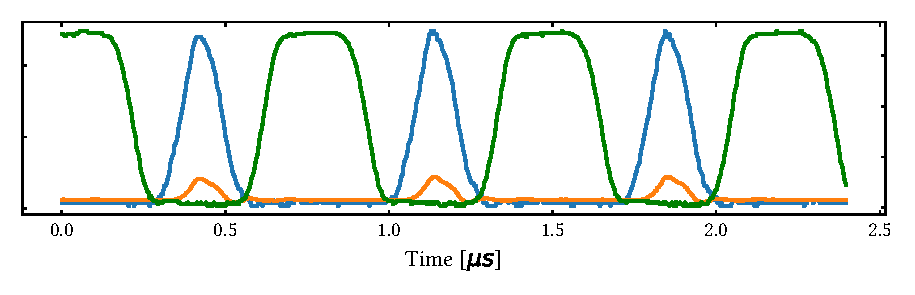
\includegraphics{figures/chopping_155.pdf}
	\caption{Chopping in the experiment. Laser beams alternate between each other, with blue being the MOT cooler, orange the MOT repumper and green the SLM tweezer. The amplitude of the MOT beams is limited due to the risetime of the \acp{aom}.}
}
\end{figure}
\todo{acronyms? MOT, SLM}

Achieving larger duty cycles and higher chopping frequencies is possible by using \acp{eom}, which are not limited by acoustic waves. The optical medium is modulated using electric fields, and in fact, can be switched as fast as common condensators. Light entering the modulator will have its polarization turned, depending on the electric field that is applied. Therefore, in the following, polarization of electro-magnetic waves is discussed briefly, which is followed by the main effect governing the devices tested in this thesis - the pockels effect. The devices are then evaluated by filtering one polarization component and the rise times and extinction ratio measured. The new system will be able to switch with rise times on the order of nanoseconds, improving the current system by at least two orders of magnitude.

The devices tested in this thesis are both capable of switching on nanosecond scales, improving the current chopping rate by three orders of magnitude. The theory behind the linear electro-optical effect is discussed after a short recourse on polarization of electromagnetic waves. Lastly, experimental evaluations for two \acp{eom} are presented and discussed.

\todo{say something about that chopping reduces lifetime}


\section{Theory on Polarization}

\label{sec:pol}

Switching laser beams using \acp{eom} means turning and filtering the polarization of the light. Therefore in the following is discussed the theory behind polarized monochromatic electromagnetic waves, leading to the pockels effect governing \acp{eom}.

Polarization of electromagnetic waves is understood as the orientation of the wave in space, transverse to the direction of movement. In general, a wave travelling along the z-axis can be oriented somewhere in the x-y plane. Therefore, writing the electric field component of the light in this basis takes the following form:

\begin{equation}
	\mathbf{E}(\mathbf{x}, t) = E_x cos\left(kx - wt + \phi_x\right) \mathbf{e_x} + E_y cos\left(ky - wt + \phi_y\right) \mathbf{e_y} .
\end{equation}

Here, $k$ and $w$ refer to the wave number and frequency respectively.
Depending on the amplitudes $E_x$ and $E_y$ and the phases $\phi_x$ and $\phi_y$, the wave can be in different polarization states. If it is not possible to write the wave in this basis, the light is unpolarized. Otherwise, it is \textbf{linear}, when either one of the amplitudes $E_x$ or $E_y$ is zero or when the phase difference $\Delta \phi = \phi_x - \phi_y$ evaluates to 0 or $\pi$. It is \textbf{circular}, when the phase difference $\Delta \phi = \pm \pi/2$ and the amplitudes are the same, $E_x = E_y$. In any other case, the wave is \textbf{elliptically} polarized.

By changing the phases of the wave relative to each other therefore gives the ability to affect the polarization. Light traversing a medium will accumulate a phase shift, depending on the refractive index, which affects the speed of light in the medium. Therefore, media that have different refractive indices $n_x, n_y$ along the two axes $x$ and $y$ means changing the relative phases of the wave:

\begin{align}
	\label{eq:pol,phases}
	\phi_x(z) = k_0 n_x z \\
	\phi_y(z) = k_0 n_y z
\end{align}

where $k_0$ is the free space wave vector of the light. Then a device that retards the phase difference $\Delta \phi$ by $\pi/2$, which is a quarter of the wavelength, can change linearly polarized light to circularly polarized light (or vice-versa) and is therefore called a $\lambda / 4$ waveplate. Similarily, if the phase difference is changed by $\Delta \phi = \pi$, or a half wavelength, then we can turn linear polarization around a given axis or change the orientation of circularly polarized light. This is then called a $\lambda / 2$ waveplate. In the experiment, linearly polarized light will enter the \ac{eom}, which will act as a $\lambda / 2$ waveplate, turning the polarization by $\SI{90}{\degree}$, making it easy to filter unwanted polarization components and switching the light on and off.

\section{Electro-optical modulators}
\label{sec:eom}

Light travelling through a material generally has a speed smaller than the speed of light. This property of the material is the refractive index and is the ratio of the speed of light in the material to the speed of light in vacuum. Materials can change their refractive index by being exposed to an electric field, which in \acp{eom} is generally a crystal connected to two electrodes. There are two prominent electro-optical effects that need to be distinguished. If the refractive index changes linearly with the electric field, the effect is called Pockels effect and the \ac{eom} is called a pockels cell. The effect is discussed in the following and the pockels cells evaluated afterwards.

\subsection{Pockels effect}
\label{sec:pockels_effect}

As was motivated in the previous section, the goal of modulating light polarization is to change the relative refractive index of a medium in two axes. Following the argumentation from the book Fundamentals of Photonics \cite{Saleh1991}, the pockels effect can be found by evaluating the refractive index with respect to the electric field applied to the modulator. Writing this as $n(E)$ and applying a taylor expansion, we get the following expression:

\begin{equation}
	n(E) = n_0 + \frac{dn}{dE} E + \mathcal{O}(E^2)
\end{equation}

The pockels effect is the linear dependence of the refractive index to the electric field, therefore higher orders are neglected. The prefactor $dn / dE$ can be found from the change of electric impermeability $\Delta \eta$, which is the ability of a material to be penetrated by an electromagnetic field. From

\begin{align}
	\eta & = \frac{1}{n^2},
\end{align}
we get
\begin{align}
	\label{eq:pockel,refr}
	\Delta \eta = \frac{d \eta}{dn} \Delta n & = -\frac{2}{n_0^3} \frac{dn}{dE} E = \mathfrak{r} E .
\end{align}

This results in the quantity $\mathfrak{r} = -\frac{2}{n_0^3} \frac{dn}{dE}$, which is called the Pockels coefficient given in units of $\SI{}{\meter\per\volt}$. It can be measured by evaluating the refractive index of the material:

\begin{equation}
	n(E) = n_0 - \frac{1}{2} \mathfrak{r} n_0^3 E .
\end{equation}

As was seen in Equation \ref{eq:pol,phases}, the refractive index directly affects the phase shift, which in turn changes the polarization of the light wave. Combining the results leads to an equation using parameters typically found in \acp{eom}:

\begin{align}
	\phi & = k_0 L n \\
		 & = k_0 L n_0 - \frac{k_0}{2} L \mathfrak{r} n_0^3 E \\
		 & = \phi_0 - \frac{k_0}{2} L \mathfrak{r} n_0^3 E \\
		 & = \phi_0 - \frac{\pi}{\lambda_0} L \mathfrak{r} n_0^3 E
\end{align}

where the relation $k_0 = 2 \pi / \lambda_0$ of the wave number was used.

The pockels cells in this application act as dynamic wave retarders, therefore with the results from Section~\ref{sec:pol}, we can tune the phase difference $\Delta \phi = \phi_x - \phi_y$ along the axes $x$ and $y$ by applying an electric field. With the correct parameters, the phase difference lets the \ac{eom} act as a $\lambda / 2$ or $\lambda / 4$ waveplate. The following relations will help find the main formula governing pockels cells, resulting in the voltage that needs to be applied to the \ac{eom} in order to turn the polarization a given amount.

Labeling the refractive index in two dimensions as:

\begin{align}
	n_x(E) = n_{0,x} - \frac{1}{2} \mathfrak{r}_x n_{0,x}^3 E \\
	n_y(E) = n_{0,y} - \frac{1}{2} \mathfrak{r}_y n_{0,y}^3 E
\end{align}

then the phase difference becomes:

\begin{align}
	\Delta \phi & = \phi_{0,x} - \phi_{0,y} - \frac{\pi}{\lambda_0} E L \left(\mathfrak{r}_x n_x^3 - \mathfrak{r}_y n_y^3\right) \\
	\Delta \phi & = \Delta \phi_{0} - \frac{\pi}{\lambda_0} E L \left(\mathfrak{r}_x n_x^3 - \mathfrak{r}_y n_y^3\right) .
	\label{eq:eom_phase_diff}
\end{align}

\begin{figure}[t]
\centering{
	\import{figures}{eom_schematic.pdf_tex}
	\caption{Schematic view of light passing through an \ac{eom} of length $L$. The electrodes are positioned on the front and back side of the modulator, the same faces the light enters and exits. The light exiting the \ac{eom} has a relative phase shift $\Delta \Phi$ depending on the change of refractive index due to the applied voltage $V$.}
\label{fig:eom_schem}
}
\end{figure}

The next step is to replace the electric field by a voltage that can be applied to the pockels cell. For this, two electrodes are connected to the \ac{eom}, separated by a distance $d$. This gives the electric field as $E=V/d$. This quantity is replaced into Equation~\ref{eq:eom_phase_diff} and by realizing that the phase is unitless, all other prefactors of the voltage can be combined into one quantity, called the half-wave voltage $V_\pi$:

\begin{align}
	V_\pi = \frac{d}{L} \frac{\lambda_0}{\mathfrak{r}_x n_x^3 - \mathfrak{r}_y n_y^3}.
\end{align}

Thus, the phase difference can be rewritten as:

\begin{align}
	\label{eq:eom_phase_diff}
	\Delta \phi = \Delta \phi_0 - \pi \frac{V}{V_\pi} .
\end{align}

With this it is clear, that applying the voltage $V_\pi$, the pockels cell will act as a lambda-half waveplate. A visual represantation of the modulator and the light passing through it is given in Figure \ref{fig:eom_schem}, highlighting the change in relative phase of the two components of the electro-magnetic wave.

We have seen, how applying a voltage to an electro-optical medium changes the refractive index and therefore affects the phase of an electromagnetic wave. By having two refractive indices in two axes, whose relative change depends on the applied voltage, it is therefore possible to modify the circularity and linearity of the polarization in an \acl{eom}.

\subsection{Driving a pockels cell}

Rise and fall times of pockels cells can go as low as nanoseconds. To make use of this speed, one has to deploy clever ways to drive the voltages, especially when these potentials are in the kilovolt-regime. For the two Pockels cells discussed in this thesis, specialized drivers by BME-Bergmann were used.

Schematically, the driver is divided into four inputs that are controlled from the user: ON A, ON B, OFF A and OFF B. These inputs control switches on either side of the pockels cell, so A controls one electrode and B the other. Most importantly, the ON X and OFF X (X referring to either A or B) switches work exclusively, so sending a high to ON X will also send a low to OFF X and vice-versa. It is then possible to apply either a positive high voltage or a negative high voltage, depending on the state of the switches. For full identification of the circuit, which is given in Figure \ref{fig:eom_driver_switches}, the side containing the positive voltage information is called high side and similarily the side containing the negative voltage information is called low side.

A requirement for our experiment is to have the \acp{eom} work consistently. This means it is preferrable to only apply one type of voltage, because it can not be guaranteed that applying the same voltage with different polarity results in the same shift polarization. Most notably, the linearly polarized light has to be perfectly aligned on the axis of the EOM to rotate it $\SI{90}{\degree}$ in either direction, as the polarization may drift with time.

This means, only positive voltages will be applied, which results in the timing diagrams in Figure \ref{fig:eom_timings}.

\begin{figure}[t]
\centering{
	\begin{multicols}{2}
	\import{figures}{bpp_switches.pdf_tex}
	\import{figures}{dpp_switches.pdf_tex}
	\end{multicols}
	\caption{Schematic of the high voltage switches used inside the bpp-type (left) and dpp-type (right) pockels cell driver from BME Bergmann. Not-Gates on both A and B sides ensure that there is always a potential over the pockels cell. The blue and red paths indicate the connection to apply a positive and negative voltage over the pockels cell respectively.}
\label{fig:eom_driver_switches}
}
\end{figure}

\begin{figure}[t]
\centering{
	\import{figures}{bpp_timings.pdf_tex}
	\caption{Timing diagrams for the pockels cell drivers to turn the polarization of the \ac{eom} $\SI{90}{\degree}$. To get a positive high voltage from the bpp-type driver, the A and B side ON/OFF switches are flipped simultaneously. The dpp-type driver is more flexible, since it also allows negative voltages. The timings displayed here are an example to only apply positive voltages across the pockels cell.}
\label{fig:eom_timings}
}
\end{figure}

\subsection{Evaluation of Leysop Pockels cells}

The following pockels cells from Leysop Ltd. were chosen with the application in mind of switching light on the nanoseond scale on and off. Pockels cells can fulfill this requirement by exploiting the fact that linearly polarized light can be filtered out. This is best achieved by placing a \ac{pbs} directly after the modulator as seen in Figure \ref{fig:eom_setup}. This way, the setup can be configured such that applying no voltage means light passes through the beam splitter, while applying $V_\pi$ means the light gets reflected $\SI{90}{\degree}$ off the beam splitter.
Two  pockels cells were characterized by placing a photodiode on one end of the beam splitter. The \acp{eom} are labeled by the material of their nonlinear crystal, \ac{rtp} and \ac{bbo}. Their characteristics are summarized in table \ref{tbl:eom_crystals}.

\begin{figure}[t]
	\label{fig:eom_setup}
\centering{
	\import{figures}{eom_setup.pdf_tex}
	\caption{The efficiency of the \acp{eom} were evaluated by setting the polarization of the incoming light either horizontal or vertical using the waveplate. The pockels cell will then periodically turn the polarization $\SI{90}{\degree}$, which can be seen by measuring the voltage on the photodiode.}
\label{fig:eom_timings}
}
\end{figure}

\begin{table}
\label{tbl:eom_crystals}
\centering
\begin{tabular}{l|l|l}
	\hline \hline
                                                                                     & RTP                                       & BBO \\ \thickhline
Aperture (crystal dimensions)                                                        & $\SI{3}{\milli\meter}$                    & $\SI{3}{\milli\meter}$   \\ \hline
Total crystal length (2 crystals)                                                    & $\SI{30}{\milli\meter}$                   & $\SI{50}{\milli\meter}$    \\ \hline
\begin{tabular}[c]{@{}l@{}}Approximate half wave voltage\\  (1064nm)\end{tabular}    & $\SI{1.0}{\kilo \volt}$                   & $\SI{2.8}{\kilo\volt}$    \\ \hline
%Typical dynamic extinction ratio (1064nm)                                           & $> 200:1$                                 &     \\ \hline
\begin{tabular}[c]{@{}l@{}}Peak damage threshold (1064nm, 1ns \\ pulse)\end{tabular} & $> \SI{1}{\giga \watt \per \cm \squared}$ & $> \SI{1}{\giga \watt \per \cm \squared}$   \\ \hline
Insertion loss                                                                       & $< \SI{2}{\percent}$                      & $< \SI{1.5}{\percent} $ \\ \hline \hline
\end{tabular}
\caption{Characteristics of the two pockels cells with their respective non-linear crystal materials being RTP and BBO. The aperture, damage threshold and insertion loss are given for future reference.}
\end{table}

Example traces for the \ac{rtp} and \ac{bbo} are given in Figure \ref{fig:eom_example_traces}. The peak at the start of the switch is an artifact of the photodiode. Moreover, the rise and fall times could not be resolved due to the limitations of the photodiode, a home-built model with a bandwidth of roughly $\SI{22}{\mega \hertz}$. However, Bergmann BME lists rise and fall times of various pockels cells \cite{Bergmann2020}, including the ones tested here.

\begin{figure}[t]
\label{fig:eom_example_traces}
\centering{
	\setlength{\figureheight}{2in}
	\setlength{\figurewidth}{\textwidth/2-2.5em}
	%% This file was created by tikzplotlib v0.9.4.
\begin{tikzpicture}

\definecolor{color0}{rgb}{0.12156862745098,0.466666666666667,0.705882352941177}

\begin{groupplot}[group style={group size=2 by 1, horizontal sep=5em}]
\nextgroupplot[
height=\figureheight,
minor xtick={},
minor ytick={},
scaled y ticks=false,
tick align=inside,
tick pos=both,
width=\figurewidth,
x grid style={white!69.0196078431373!black},
xlabel={Time (ms)},
xmin=-0.05, xmax=2.35,
xtick style={color=black},
xtick={-0.5,0,0.5,1,1.5,2,2.5},
y grid style={white!69.0196078431373!black},
y tick label style={/pgf/number format/fixed},
ylabel style={align=center},
ylabel={Amplitude (a. u.)},
ymin=0.2738, ymax=0.9382,
ytick style={color=black},
ytick={0.2,0.4,0.6,0.8,1}
]
\addplot [line width=1.5pt, color0]
table {%
0 0.868
0.001 0.872
0.002 0.868
0.003 0.868
0.004 0.868
0.005 0.872
0.006 0.868
0.007 0.868
0.008 0.868
0.009 0.872
0.01 0.868
0.011 0.872
0.012 0.868
0.013 0.868
0.014 0.868
0.015 0.872
0.016 0.872
0.017 0.872
0.018 0.868
0.019 0.868
0.02 0.868
0.021 0.872
0.022 0.868
0.023 0.868
0.024 0.868
0.025 0.868
0.026 0.868
0.027 0.876
0.028 0.872
0.029 0.868
0.03 0.868
0.031 0.872
0.032 0.872
0.033 0.872
0.034 0.868
0.035 0.868
0.036 0.872
0.037 0.872
0.038 0.872
0.039 0.872
0.04 0.868
0.041 0.872
0.042 0.868
0.043 0.872
0.044 0.868
0.045 0.872
0.046 0.872
0.047 0.872
0.048 0.868
0.049 0.868
0.05 0.868
0.051 0.876
0.052 0.872
0.053 0.872
0.054 0.868
0.055 0.872
0.056 0.868
0.057 0.872
0.058 0.872
0.059 0.872
0.06 0.872
0.061 0.872
0.062 0.872
0.063 0.872
0.064 0.868
0.065 0.872
0.066 0.868
0.067 0.876
0.068 0.872
0.069 0.872
0.07 0.868
0.071 0.872
0.072 0.868
0.073 0.872
0.074 0.868
0.075 0.872
0.076 0.868
0.077 0.872
0.078 0.872
0.079 0.872
0.08 0.872
0.081 0.872
0.082 0.868
0.083 0.872
0.084 0.872
0.085 0.872
0.086 0.872
0.087 0.876
0.088 0.868
0.089 0.872
0.09 0.868
0.091 0.868
0.092 0.868
0.093 0.868
0.094 0.868
0.095 0.872
0.096 0.868
0.097 0.868
0.098 0.868
0.099 0.872
0.1 0.868
0.101 0.868
0.102 0.868
0.103 0.868
0.104 0.868
0.105 0.868
0.106 0.868
0.107 0.868
0.108 0.864
0.109 0.868
0.11 0.864
0.111 0.864
0.112 0.868
0.113 0.872
0.114 0.868
0.115 0.872
0.116 0.868
0.117 0.872
0.118 0.868
0.119 0.868
0.12 0.864
0.121 0.868
0.122 0.868
0.123 0.872
0.124 0.868
0.125 0.864
0.126 0.868
0.127 0.868
0.128 0.868
0.129 0.868
0.13 0.864
0.131 0.864
0.132 0.864
0.133 0.868
0.134 0.868
0.135 0.868
0.136 0.868
0.137 0.872
0.138 0.868
0.139 0.868
0.14 0.864
0.141 0.872
0.142 0.872
0.143 0.872
0.144 0.864
0.145 0.864
0.146 0.86
0.147 0.84
0.148 0.78
0.149 0.684
0.15 0.552
0.151 0.432
0.152 0.344
0.153 0.312
0.154 0.308
0.155 0.316
0.156 0.344
0.157 0.368
0.158 0.376
0.159 0.384
0.16 0.388
0.161 0.38
0.162 0.368
0.163 0.368
0.164 0.364
0.165 0.364
0.166 0.36
0.167 0.368
0.168 0.364
0.169 0.36
0.17 0.364
0.171 0.364
0.172 0.36
0.173 0.356
0.174 0.36
0.175 0.36
0.176 0.36
0.177 0.364
0.178 0.364
0.179 0.36
0.18 0.36
0.181 0.36
0.182 0.356
0.183 0.356
0.184 0.356
0.185 0.352
0.186 0.356
0.187 0.36
0.188 0.36
0.189 0.356
0.19 0.352
0.191 0.352
0.192 0.352
0.193 0.356
0.194 0.356
0.195 0.352
0.196 0.352
0.197 0.356
0.198 0.356
0.199 0.356
0.2 0.356
0.201 0.36
0.202 0.356
0.203 0.356
0.204 0.348
0.205 0.34
0.206 0.34
0.207 0.344
0.208 0.348
0.209 0.352
0.21 0.352
0.211 0.352
0.212 0.356
0.213 0.352
0.214 0.348
0.215 0.352
0.216 0.348
0.217 0.344
0.218 0.348
0.219 0.348
0.22 0.344
0.221 0.348
0.222 0.348
0.223 0.348
0.224 0.348
0.225 0.348
0.226 0.352
0.227 0.348
0.228 0.344
0.229 0.348
0.23 0.344
0.231 0.348
0.232 0.348
0.233 0.344
0.234 0.344
0.235 0.348
0.236 0.344
0.237 0.34
0.238 0.344
0.239 0.348
0.24 0.344
0.241 0.348
0.242 0.344
0.243 0.344
0.244 0.344
0.245 0.348
0.246 0.34
0.247 0.344
0.248 0.344
0.249 0.344
0.25 0.344
0.251 0.344
0.252 0.344
0.253 0.344
0.254 0.344
0.255 0.34
0.256 0.34
0.257 0.344
0.258 0.34
0.259 0.344
0.26 0.344
0.261 0.344
0.262 0.344
0.263 0.344
0.264 0.344
0.265 0.344
0.266 0.34
0.267 0.344
0.268 0.344
0.269 0.344
0.27 0.344
0.271 0.344
0.272 0.344
0.273 0.344
0.274 0.344
0.275 0.344
0.276 0.344
0.277 0.344
0.278 0.344
0.279 0.344
0.28 0.344
0.281 0.344
0.282 0.344
0.283 0.344
0.284 0.344
0.285 0.344
0.286 0.344
0.287 0.34
0.288 0.344
0.289 0.348
0.29 0.348
0.291 0.344
0.292 0.344
0.293 0.344
0.294 0.344
0.295 0.34
0.296 0.34
0.297 0.344
0.298 0.344
0.299 0.348
0.3 0.34
0.301 0.344
0.302 0.344
0.303 0.344
0.304 0.344
0.305 0.348
0.306 0.344
0.307 0.344
0.308 0.344
0.309 0.348
0.31 0.348
0.311 0.348
0.312 0.344
0.313 0.344
0.314 0.344
0.315 0.348
0.316 0.348
0.317 0.348
0.318 0.348
0.319 0.348
0.32 0.344
0.321 0.344
0.322 0.344
0.323 0.348
0.324 0.344
0.325 0.344
0.326 0.344
0.327 0.344
0.328 0.348
0.329 0.344
0.33 0.344
0.331 0.344
0.332 0.348
0.333 0.344
0.334 0.344
0.335 0.348
0.336 0.344
0.337 0.344
0.338 0.344
0.339 0.348
0.34 0.348
0.341 0.344
0.342 0.344
0.343 0.348
0.344 0.348
0.345 0.344
0.346 0.344
0.347 0.344
0.348 0.344
0.349 0.344
0.35 0.344
0.351 0.344
0.352 0.344
0.353 0.344
0.354 0.344
0.355 0.344
0.356 0.34
0.357 0.34
0.358 0.344
0.359 0.344
0.36 0.34
0.361 0.34
0.362 0.34
0.363 0.344
0.364 0.344
0.365 0.344
0.366 0.344
0.367 0.344
0.368 0.344
0.369 0.344
0.37 0.348
0.371 0.344
0.372 0.34
0.373 0.34
0.374 0.344
0.375 0.344
0.376 0.344
0.377 0.344
0.378 0.34
0.379 0.344
0.38 0.344
0.381 0.344
0.382 0.344
0.383 0.344
0.384 0.344
0.385 0.34
0.386 0.344
0.387 0.344
0.388 0.34
0.389 0.344
0.39 0.344
0.391 0.344
0.392 0.344
0.393 0.344
0.394 0.34
0.395 0.344
0.396 0.34
0.397 0.344
0.398 0.34
0.399 0.34
0.4 0.344
0.401 0.344
0.402 0.344
0.403 0.344
0.404 0.34
0.405 0.34
0.406 0.344
0.407 0.348
0.408 0.344
0.409 0.344
0.41 0.34
0.411 0.34
0.412 0.34
0.413 0.344
0.414 0.344
0.415 0.344
0.416 0.34
0.417 0.34
0.418 0.34
0.419 0.344
0.42 0.344
0.421 0.34
0.422 0.34
0.423 0.344
0.424 0.344
0.425 0.344
0.426 0.34
0.427 0.34
0.428 0.34
0.429 0.344
0.43 0.344
0.431 0.34
0.432 0.336
0.433 0.34
0.434 0.34
0.435 0.344
0.436 0.344
0.437 0.344
0.438 0.34
0.439 0.344
0.44 0.344
0.441 0.34
0.442 0.34
0.443 0.34
0.444 0.34
0.445 0.344
0.446 0.34
0.447 0.344
0.448 0.34
0.449 0.34
0.45 0.34
0.451 0.344
0.452 0.344
0.453 0.344
0.454 0.34
0.455 0.34
0.456 0.34
0.457 0.34
0.458 0.34
0.459 0.34
0.46 0.34
0.461 0.34
0.462 0.34
0.463 0.34
0.464 0.336
0.465 0.34
0.466 0.34
0.467 0.34
0.468 0.34
0.469 0.336
0.47 0.336
0.471 0.336
0.472 0.336
0.473 0.336
0.474 0.336
0.475 0.34
0.476 0.34
0.477 0.34
0.478 0.34
0.479 0.34
0.48 0.34
0.481 0.34
0.482 0.336
0.483 0.34
0.484 0.34
0.485 0.34
0.486 0.336
0.487 0.336
0.488 0.34
0.489 0.336
0.49 0.336
0.491 0.336
0.492 0.34
0.493 0.34
0.494 0.336
0.495 0.336
0.496 0.336
0.497 0.336
0.498 0.336
0.499 0.336
0.5 0.336
0.501 0.336
0.502 0.34
0.503 0.34
0.504 0.336
0.505 0.336
0.506 0.336
0.507 0.336
0.508 0.332
0.509 0.332
0.51 0.336
0.511 0.336
0.512 0.332
0.513 0.336
0.514 0.332
0.515 0.332
0.516 0.332
0.517 0.332
0.518 0.332
0.519 0.336
0.52 0.332
0.521 0.332
0.522 0.332
0.523 0.332
0.524 0.332
0.525 0.332
0.526 0.328
0.527 0.332
0.528 0.332
0.529 0.332
0.53 0.332
0.531 0.332
0.532 0.332
0.533 0.332
0.534 0.332
0.535 0.332
0.536 0.332
0.537 0.332
0.538 0.328
0.539 0.332
0.54 0.332
0.541 0.328
0.542 0.332
0.543 0.328
0.544 0.328
0.545 0.328
0.546 0.332
0.547 0.332
0.548 0.328
0.549 0.328
0.55 0.328
0.551 0.328
0.552 0.328
0.553 0.328
0.554 0.328
0.555 0.328
0.556 0.324
0.557 0.324
0.558 0.332
0.559 0.328
0.56 0.328
0.561 0.328
0.562 0.328
0.563 0.332
0.564 0.328
0.565 0.328
0.566 0.328
0.567 0.324
0.568 0.328
0.569 0.328
0.57 0.332
0.571 0.328
0.572 0.324
0.573 0.328
0.574 0.328
0.575 0.328
0.576 0.324
0.577 0.328
0.578 0.328
0.579 0.328
0.58 0.328
0.581 0.328
0.582 0.328
0.583 0.328
0.584 0.324
0.585 0.328
0.586 0.328
0.587 0.324
0.588 0.32
0.589 0.324
0.59 0.328
0.591 0.328
0.592 0.328
0.593 0.328
0.594 0.324
0.595 0.328
0.596 0.332
0.597 0.328
0.598 0.328
0.599 0.332
0.6 0.328
0.601 0.328
0.602 0.324
0.603 0.332
0.604 0.332
0.605 0.332
0.606 0.328
0.607 0.332
0.608 0.332
0.609 0.332
0.61 0.328
0.611 0.332
0.612 0.328
0.613 0.332
0.614 0.328
0.615 0.332
0.616 0.328
0.617 0.332
0.618 0.328
0.619 0.328
0.62 0.332
0.621 0.336
0.622 0.328
0.623 0.332
0.624 0.332
0.625 0.332
0.626 0.328
0.627 0.328
0.628 0.328
0.629 0.332
0.63 0.332
0.631 0.332
0.632 0.328
0.633 0.332
0.634 0.328
0.635 0.332
0.636 0.328
0.637 0.332
0.638 0.328
0.639 0.332
0.64 0.332
0.641 0.332
0.642 0.332
0.643 0.332
0.644 0.332
0.645 0.332
0.646 0.328
0.647 0.332
0.648 0.328
0.649 0.332
0.65 0.352
0.651 0.408
0.652 0.512
0.653 0.648
0.654 0.764
0.655 0.848
0.656 0.892
0.657 0.908
0.658 0.896
0.659 0.88
0.66 0.864
0.661 0.852
0.662 0.844
0.663 0.844
0.664 0.848
0.665 0.852
0.666 0.856
0.667 0.86
0.668 0.856
0.669 0.856
0.67 0.86
0.671 0.864
0.672 0.86
0.673 0.864
0.674 0.86
0.675 0.864
0.676 0.86
0.677 0.864
0.678 0.86
0.679 0.864
0.68 0.86
0.681 0.86
0.682 0.86
0.683 0.864
0.684 0.86
0.685 0.864
0.686 0.864
0.687 0.868
0.688 0.864
0.689 0.864
0.69 0.86
0.691 0.864
0.692 0.86
0.693 0.864
0.694 0.864
0.695 0.868
0.696 0.864
0.697 0.868
0.698 0.868
0.699 0.868
0.7 0.864
0.701 0.864
0.702 0.86
0.703 0.86
0.704 0.86
0.705 0.86
0.706 0.86
0.707 0.872
0.708 0.876
0.709 0.876
0.71 0.872
0.711 0.868
0.712 0.864
0.713 0.868
0.714 0.86
0.715 0.86
0.716 0.864
0.717 0.868
0.718 0.868
0.719 0.872
0.72 0.868
0.721 0.864
0.722 0.868
0.723 0.872
0.724 0.868
0.725 0.864
0.726 0.864
0.727 0.868
0.728 0.868
0.729 0.868
0.73 0.864
0.731 0.868
0.732 0.868
0.733 0.868
0.734 0.864
0.735 0.868
0.736 0.864
0.737 0.868
0.738 0.868
0.739 0.868
0.74 0.868
0.741 0.868
0.742 0.868
0.743 0.868
0.744 0.864
0.745 0.868
0.746 0.868
0.747 0.868
0.748 0.868
0.749 0.868
0.75 0.864
0.751 0.864
0.752 0.864
0.753 0.868
0.754 0.868
0.755 0.868
0.756 0.864
0.757 0.864
0.758 0.864
0.759 0.868
0.76 0.868
0.761 0.864
0.762 0.864
0.763 0.872
0.764 0.872
0.765 0.872
0.766 0.864
0.767 0.868
0.768 0.868
0.769 0.868
0.77 0.868
0.771 0.872
0.772 0.868
0.773 0.868
0.774 0.868
0.775 0.868
0.776 0.868
0.777 0.872
0.778 0.868
0.779 0.868
0.78 0.868
0.781 0.868
0.782 0.868
0.783 0.868
0.784 0.864
0.785 0.868
0.786 0.868
0.787 0.868
0.788 0.868
0.789 0.868
0.79 0.868
0.791 0.864
0.792 0.864
0.793 0.868
0.794 0.864
0.795 0.868
0.796 0.864
0.797 0.868
0.798 0.864
0.799 0.868
0.8 0.868
0.801 0.872
0.802 0.872
0.803 0.872
0.804 0.868
0.805 0.872
0.806 0.868
0.807 0.868
0.808 0.868
0.809 0.876
0.81 0.872
0.811 0.872
0.812 0.868
0.813 0.868
0.814 0.868
0.815 0.868
0.816 0.864
0.817 0.868
0.818 0.864
0.819 0.872
0.82 0.872
0.821 0.872
0.822 0.868
0.823 0.872
0.824 0.868
0.825 0.868
0.826 0.864
0.827 0.868
0.828 0.868
0.829 0.868
0.83 0.868
0.831 0.872
0.832 0.868
0.833 0.872
0.834 0.868
0.835 0.872
0.836 0.872
0.837 0.872
0.838 0.868
0.839 0.872
0.84 0.868
0.841 0.868
0.842 0.868
0.843 0.868
0.844 0.868
0.845 0.868
0.846 0.868
0.847 0.868
0.848 0.868
0.849 0.872
0.85 0.872
0.851 0.872
0.852 0.868
0.853 0.868
0.854 0.868
0.855 0.868
0.856 0.868
0.857 0.872
0.858 0.868
0.859 0.868
0.86 0.864
0.861 0.872
0.862 0.868
0.863 0.868
0.864 0.868
0.865 0.868
0.866 0.868
0.867 0.868
0.868 0.868
0.869 0.868
0.87 0.868
0.871 0.872
0.872 0.868
0.873 0.868
0.874 0.864
0.875 0.864
0.876 0.868
0.877 0.868
0.878 0.868
0.879 0.872
0.88 0.872
0.881 0.872
0.882 0.868
0.883 0.872
0.884 0.864
0.885 0.872
0.886 0.868
0.887 0.872
0.888 0.868
0.889 0.872
0.89 0.868
0.891 0.872
0.892 0.868
0.893 0.868
0.894 0.868
0.895 0.872
0.896 0.872
0.897 0.872
0.898 0.868
0.899 0.872
0.9 0.868
0.901 0.868
0.902 0.868
0.903 0.872
0.904 0.864
0.905 0.868
0.906 0.868
0.907 0.868
0.908 0.868
0.909 0.872
0.91 0.868
0.911 0.868
0.912 0.868
0.913 0.872
0.914 0.868
0.915 0.868
0.916 0.868
0.917 0.876
0.918 0.872
0.919 0.872
0.92 0.868
0.921 0.872
0.922 0.872
0.923 0.876
0.924 0.872
0.925 0.872
0.926 0.868
0.927 0.872
0.928 0.868
0.929 0.868
0.93 0.868
0.931 0.868
0.932 0.868
0.933 0.876
0.934 0.868
0.935 0.872
0.936 0.872
0.937 0.872
0.938 0.872
0.939 0.872
0.94 0.872
0.941 0.876
0.942 0.876
0.943 0.876
0.944 0.872
0.945 0.872
0.946 0.872
0.947 0.876
0.948 0.868
0.949 0.872
0.95 0.868
0.951 0.868
0.952 0.868
0.953 0.868
0.954 0.868
0.955 0.872
0.956 0.868
0.957 0.868
0.958 0.868
0.959 0.872
0.96 0.872
0.961 0.872
0.962 0.868
0.963 0.868
0.964 0.868
0.965 0.872
0.966 0.872
0.967 0.876
0.968 0.872
0.969 0.872
0.97 0.872
0.971 0.872
0.972 0.868
0.973 0.868
0.974 0.868
0.975 0.868
0.976 0.868
0.977 0.868
0.978 0.868
0.979 0.868
0.98 0.868
0.981 0.868
0.982 0.868
0.983 0.868
0.984 0.864
0.985 0.868
0.986 0.868
0.987 0.868
0.988 0.868
0.989 0.868
0.99 0.868
0.991 0.868
0.992 0.868
0.993 0.868
0.994 0.868
0.995 0.868
0.996 0.868
0.997 0.868
0.998 0.868
0.999 0.868
1 0.868
1.001 0.868
1.002 0.868
1.003 0.868
1.004 0.868
1.005 0.868
1.006 0.864
1.007 0.864
1.008 0.868
1.009 0.868
1.01 0.864
1.011 0.864
1.012 0.864
1.013 0.868
1.014 0.868
1.015 0.868
1.016 0.868
1.017 0.868
1.018 0.864
1.019 0.868
1.02 0.868
1.021 0.872
1.022 0.872
1.023 0.872
1.024 0.868
1.025 0.872
1.026 0.868
1.027 0.872
1.028 0.872
1.029 0.868
1.03 0.868
1.031 0.872
1.032 0.872
1.033 0.868
1.034 0.864
1.035 0.868
1.036 0.868
1.037 0.872
1.038 0.868
1.039 0.868
1.04 0.868
1.041 0.868
1.042 0.868
1.043 0.868
1.044 0.868
1.045 0.868
1.046 0.868
1.047 0.868
1.048 0.864
1.049 0.868
1.05 0.868
1.051 0.868
1.052 0.868
1.053 0.868
1.054 0.872
1.055 0.872
1.056 0.868
1.057 0.864
1.058 0.864
1.059 0.868
1.06 0.868
1.061 0.864
1.062 0.864
1.063 0.868
1.064 0.864
1.065 0.864
1.066 0.86
1.067 0.864
1.068 0.864
1.069 0.868
1.07 0.864
1.071 0.864
1.072 0.864
1.073 0.868
1.074 0.864
1.075 0.868
1.076 0.868
1.077 0.868
1.078 0.868
1.079 0.868
1.08 0.868
1.081 0.864
1.082 0.864
1.083 0.864
1.084 0.864
1.085 0.868
1.086 0.864
1.087 0.868
1.088 0.864
1.089 0.864
1.09 0.86
1.091 0.868
1.092 0.864
1.093 0.868
1.094 0.864
1.095 0.868
1.096 0.864
1.097 0.868
1.098 0.864
1.099 0.864
1.1 0.868
1.101 0.868
1.102 0.864
1.103 0.868
1.104 0.868
1.105 0.868
1.106 0.864
1.107 0.868
1.108 0.868
1.109 0.876
1.11 0.868
1.111 0.868
1.112 0.864
1.113 0.868
1.114 0.868
1.115 0.868
1.116 0.868
1.117 0.868
1.118 0.864
1.119 0.868
1.12 0.868
1.121 0.868
1.122 0.864
1.123 0.868
1.124 0.868
1.125 0.864
1.126 0.864
1.127 0.868
1.128 0.868
1.129 0.868
1.13 0.868
1.131 0.872
1.132 0.868
1.133 0.872
1.134 0.872
1.135 0.868
1.136 0.868
1.137 0.872
1.138 0.868
1.139 0.868
1.14 0.868
1.141 0.868
1.142 0.868
1.143 0.868
1.144 0.864
1.145 0.868
1.146 0.864
1.147 0.864
1.148 0.84
1.149 0.78
1.15 0.672
1.151 0.54
1.152 0.424
1.153 0.348
1.154 0.308
1.155 0.308
1.156 0.324
1.157 0.34
1.158 0.36
1.159 0.38
1.16 0.384
1.161 0.376
1.162 0.372
1.163 0.372
1.164 0.364
1.165 0.36
1.166 0.364
1.167 0.364
1.168 0.364
1.169 0.364
1.17 0.36
1.171 0.356
1.172 0.356
1.173 0.36
1.174 0.36
1.175 0.356
1.176 0.36
1.177 0.36
1.178 0.36
1.179 0.36
1.18 0.356
1.181 0.356
1.182 0.356
1.183 0.356
1.184 0.352
1.185 0.356
1.186 0.356
1.187 0.356
1.188 0.352
1.189 0.356
1.19 0.356
1.191 0.352
1.192 0.352
1.193 0.356
1.194 0.356
1.195 0.352
1.196 0.352
1.197 0.352
1.198 0.348
1.199 0.352
1.2 0.352
1.201 0.356
1.202 0.36
1.203 0.356
1.204 0.352
1.205 0.348
1.206 0.336
1.207 0.34
1.208 0.344
1.209 0.348
1.21 0.352
1.211 0.356
1.212 0.352
1.213 0.344
1.214 0.344
1.215 0.348
1.216 0.344
1.217 0.348
1.218 0.348
1.219 0.348
1.22 0.344
1.221 0.344
1.222 0.344
1.223 0.348
1.224 0.348
1.225 0.344
1.226 0.34
1.227 0.344
1.228 0.348
1.229 0.344
1.23 0.344
1.231 0.344
1.232 0.344
1.233 0.344
1.234 0.34
1.235 0.34
1.236 0.344
1.237 0.348
1.238 0.344
1.239 0.34
1.24 0.344
1.241 0.344
1.242 0.34
1.243 0.344
1.244 0.344
1.245 0.344
1.246 0.34
1.247 0.344
1.248 0.344
1.249 0.34
1.25 0.34
1.251 0.34
1.252 0.34
1.253 0.348
1.254 0.344
1.255 0.344
1.256 0.344
1.257 0.348
1.258 0.344
1.259 0.344
1.26 0.34
1.261 0.34
1.262 0.344
1.263 0.344
1.264 0.34
1.265 0.34
1.266 0.34
1.267 0.34
1.268 0.344
1.269 0.344
1.27 0.34
1.271 0.34
1.272 0.34
1.273 0.34
1.274 0.34
1.275 0.34
1.276 0.34
1.277 0.344
1.278 0.34
1.279 0.34
1.28 0.34
1.281 0.34
1.282 0.34
1.283 0.34
1.284 0.336
1.285 0.336
1.286 0.344
1.287 0.344
1.288 0.344
1.289 0.34
1.29 0.34
1.291 0.344
1.292 0.34
1.293 0.34
1.294 0.344
1.295 0.344
1.296 0.344
1.297 0.344
1.298 0.344
1.299 0.344
1.3 0.344
1.301 0.34
1.302 0.34
1.303 0.344
1.304 0.34
1.305 0.34
1.306 0.34
1.307 0.34
1.308 0.344
1.309 0.344
1.31 0.344
1.311 0.34
1.312 0.344
1.313 0.34
1.314 0.34
1.315 0.344
1.316 0.344
1.317 0.34
1.318 0.344
1.319 0.348
1.32 0.348
1.321 0.344
1.322 0.34
1.323 0.344
1.324 0.344
1.325 0.34
1.326 0.34
1.327 0.344
1.328 0.344
1.329 0.344
1.33 0.344
1.331 0.34
1.332 0.344
1.333 0.34
1.334 0.34
1.335 0.34
1.336 0.344
1.337 0.344
1.338 0.34
1.339 0.34
1.34 0.344
1.341 0.344
1.342 0.344
1.343 0.344
1.344 0.344
1.345 0.34
1.346 0.344
1.347 0.348
1.348 0.344
1.349 0.34
1.35 0.344
1.351 0.344
1.352 0.34
1.353 0.34
1.354 0.344
1.355 0.348
1.356 0.344
1.357 0.34
1.358 0.34
1.359 0.344
1.36 0.34
1.361 0.344
1.362 0.34
1.363 0.344
1.364 0.344
1.365 0.34
1.366 0.34
1.367 0.34
1.368 0.34
1.369 0.344
1.37 0.34
1.371 0.34
1.372 0.34
1.373 0.34
1.374 0.34
1.375 0.34
1.376 0.34
1.377 0.34
1.378 0.34
1.379 0.34
1.38 0.34
1.381 0.344
1.382 0.344
1.383 0.344
1.384 0.34
1.385 0.34
1.386 0.344
1.387 0.34
1.388 0.34
1.389 0.34
1.39 0.344
1.391 0.348
1.392 0.344
1.393 0.34
1.394 0.34
1.395 0.344
1.396 0.34
1.397 0.34
1.398 0.34
1.399 0.34
1.4 0.34
1.401 0.344
1.402 0.344
1.403 0.344
1.404 0.344
1.405 0.34
1.406 0.34
1.407 0.34
1.408 0.34
1.409 0.344
1.41 0.34
1.411 0.34
1.412 0.336
1.413 0.34
1.414 0.344
1.415 0.344
1.416 0.344
1.417 0.344
1.418 0.344
1.419 0.344
1.42 0.34
1.421 0.34
1.422 0.34
1.423 0.344
1.424 0.344
1.425 0.34
1.426 0.336
1.427 0.34
1.428 0.344
1.429 0.344
1.43 0.344
1.431 0.34
1.432 0.34
1.433 0.34
1.434 0.34
1.435 0.34
1.436 0.34
1.437 0.34
1.438 0.34
1.439 0.34
1.44 0.34
1.441 0.34
1.442 0.34
1.443 0.34
1.444 0.34
1.445 0.336
1.446 0.336
1.447 0.34
1.448 0.336
1.449 0.336
1.45 0.336
1.451 0.34
1.452 0.336
1.453 0.34
1.454 0.34
1.455 0.336
1.456 0.336
1.457 0.336
1.458 0.34
1.459 0.34
1.46 0.34
1.461 0.34
1.462 0.34
1.463 0.34
1.464 0.34
1.465 0.336
1.466 0.34
1.467 0.336
1.468 0.336
1.469 0.34
1.47 0.34
1.471 0.34
1.472 0.336
1.473 0.336
1.474 0.332
1.475 0.336
1.476 0.336
1.477 0.336
1.478 0.336
1.479 0.336
1.48 0.336
1.481 0.34
1.482 0.34
1.483 0.336
1.484 0.336
1.485 0.336
1.486 0.336
1.487 0.34
1.488 0.336
1.489 0.336
1.49 0.336
1.491 0.336
1.492 0.332
1.493 0.336
1.494 0.336
1.495 0.336
1.496 0.332
1.497 0.336
1.498 0.332
1.499 0.336
1.5 0.336
1.501 0.332
1.502 0.332
1.503 0.336
1.504 0.336
1.505 0.336
1.506 0.332
1.507 0.336
1.508 0.336
1.509 0.336
1.51 0.332
1.511 0.332
1.512 0.328
1.513 0.332
1.514 0.332
1.515 0.336
1.516 0.332
1.517 0.332
1.518 0.328
1.519 0.332
1.52 0.332
1.521 0.328
1.522 0.328
1.523 0.332
1.524 0.328
1.525 0.328
1.526 0.328
1.527 0.332
1.528 0.332
1.529 0.332
1.53 0.328
1.531 0.332
1.532 0.332
1.533 0.328
1.534 0.328
1.535 0.328
1.536 0.328
1.537 0.328
1.538 0.328
1.539 0.324
1.54 0.324
1.541 0.328
1.542 0.328
1.543 0.328
1.544 0.324
1.545 0.328
1.546 0.328
1.547 0.328
1.548 0.328
1.549 0.328
1.55 0.328
1.551 0.328
1.552 0.328
1.553 0.328
1.554 0.328
1.555 0.328
1.556 0.328
1.557 0.328
1.558 0.324
1.559 0.328
1.56 0.328
1.561 0.328
1.562 0.328
1.563 0.324
1.564 0.32
1.565 0.324
1.566 0.328
1.567 0.328
1.568 0.324
1.569 0.324
1.57 0.32
1.571 0.32
1.572 0.328
1.573 0.328
1.574 0.324
1.575 0.324
1.576 0.324
1.577 0.328
1.578 0.324
1.579 0.32
1.58 0.324
1.581 0.328
1.582 0.324
1.583 0.324
1.584 0.324
1.585 0.328
1.586 0.324
1.587 0.324
1.588 0.324
1.589 0.328
1.59 0.328
1.591 0.328
1.592 0.324
1.593 0.328
1.594 0.328
1.595 0.332
1.596 0.328
1.597 0.328
1.598 0.328
1.599 0.332
1.6 0.324
1.601 0.328
1.602 0.328
1.603 0.328
1.604 0.324
1.605 0.324
1.606 0.324
1.607 0.328
1.608 0.324
1.609 0.324
1.61 0.324
1.611 0.328
1.612 0.328
1.613 0.328
1.614 0.328
1.615 0.332
1.616 0.328
1.617 0.328
1.618 0.324
1.619 0.328
1.62 0.328
1.621 0.328
1.622 0.324
1.623 0.328
1.624 0.328
1.625 0.332
1.626 0.324
1.627 0.328
1.628 0.328
1.629 0.332
1.63 0.328
1.631 0.328
1.632 0.332
1.633 0.332
1.634 0.328
1.635 0.328
1.636 0.328
1.637 0.324
1.638 0.324
1.639 0.328
1.64 0.328
1.641 0.328
1.642 0.328
1.643 0.328
1.644 0.328
1.645 0.328
1.646 0.324
1.647 0.32
1.648 0.328
1.649 0.332
1.65 0.34
1.651 0.388
1.652 0.48
1.653 0.604
1.654 0.728
1.655 0.82
1.656 0.876
1.657 0.9
1.658 0.896
1.659 0.884
1.66 0.864
1.661 0.844
1.662 0.84
1.663 0.84
1.664 0.84
1.665 0.848
1.666 0.852
1.667 0.852
1.668 0.856
1.669 0.852
1.67 0.856
1.671 0.856
1.672 0.856
1.673 0.856
1.674 0.856
1.675 0.86
1.676 0.86
1.677 0.856
1.678 0.856
1.679 0.852
1.68 0.856
1.681 0.852
1.682 0.856
1.683 0.86
1.684 0.86
1.685 0.864
1.686 0.864
1.687 0.86
1.688 0.856
1.689 0.86
1.69 0.86
1.691 0.86
1.692 0.864
1.693 0.864
1.694 0.86
1.695 0.86
1.696 0.86
1.697 0.864
1.698 0.864
1.699 0.864
1.7 0.86
1.701 0.86
1.702 0.86
1.703 0.856
1.704 0.852
1.705 0.856
1.706 0.86
1.707 0.864
1.708 0.868
1.709 0.868
1.71 0.864
1.711 0.864
1.712 0.86
1.713 0.86
1.714 0.86
1.715 0.86
1.716 0.86
1.717 0.86
1.718 0.86
1.719 0.864
1.72 0.868
1.721 0.868
1.722 0.86
1.723 0.86
1.724 0.86
1.725 0.864
1.726 0.86
1.727 0.864
1.728 0.864
1.729 0.864
1.73 0.86
1.731 0.864
1.732 0.86
1.733 0.864
1.734 0.864
1.735 0.86
1.736 0.86
1.737 0.864
1.738 0.864
1.739 0.864
1.74 0.864
1.741 0.864
1.742 0.864
1.743 0.864
1.744 0.86
1.745 0.864
1.746 0.86
1.747 0.86
1.748 0.86
1.749 0.864
1.75 0.864
1.751 0.86
1.752 0.86
1.753 0.864
1.754 0.86
1.755 0.864
1.756 0.868
1.757 0.864
1.758 0.86
1.759 0.864
1.76 0.86
1.761 0.864
1.762 0.864
1.763 0.864
1.764 0.864
1.765 0.864
1.766 0.86
1.767 0.864
1.768 0.864
1.769 0.864
1.77 0.86
1.771 0.86
1.772 0.864
1.773 0.86
1.774 0.864
1.775 0.864
1.776 0.864
1.777 0.864
1.778 0.864
1.779 0.864
1.78 0.86
1.781 0.864
1.782 0.864
1.783 0.864
1.784 0.864
1.785 0.864
1.786 0.864
1.787 0.864
1.788 0.864
1.789 0.864
1.79 0.864
1.791 0.864
1.792 0.86
1.793 0.864
1.794 0.86
1.795 0.864
1.796 0.864
1.797 0.864
1.798 0.856
1.799 0.86
1.8 0.864
1.801 0.864
1.802 0.864
1.803 0.868
1.804 0.868
1.805 0.864
1.806 0.86
1.807 0.86
1.808 0.86
1.809 0.864
1.81 0.86
1.811 0.86
1.812 0.864
1.813 0.864
1.814 0.86
1.815 0.86
1.816 0.86
1.817 0.864
1.818 0.864
1.819 0.864
1.82 0.86
1.821 0.86
1.822 0.86
1.823 0.86
1.824 0.86
1.825 0.864
1.826 0.864
1.827 0.864
1.828 0.864
1.829 0.864
1.83 0.864
1.831 0.864
1.832 0.864
1.833 0.864
1.834 0.86
1.835 0.864
1.836 0.86
1.837 0.86
1.838 0.86
1.839 0.864
1.84 0.86
1.841 0.864
1.842 0.864
1.843 0.864
1.844 0.864
1.845 0.864
1.846 0.864
1.847 0.864
1.848 0.86
1.849 0.86
1.85 0.868
1.851 0.868
1.852 0.864
1.853 0.864
1.854 0.86
1.855 0.864
1.856 0.864
1.857 0.864
1.858 0.864
1.859 0.864
1.86 0.864
1.861 0.864
1.862 0.864
1.863 0.868
1.864 0.868
1.865 0.864
1.866 0.864
1.867 0.864
1.868 0.864
1.869 0.864
1.87 0.864
1.871 0.868
1.872 0.868
1.873 0.868
1.874 0.864
1.875 0.864
1.876 0.868
1.877 0.864
1.878 0.864
1.879 0.868
1.88 0.868
1.881 0.868
1.882 0.864
1.883 0.868
1.884 0.864
1.885 0.864
1.886 0.864
1.887 0.864
1.888 0.864
1.889 0.864
1.89 0.864
1.891 0.864
1.892 0.864
1.893 0.868
1.894 0.868
1.895 0.868
1.896 0.868
1.897 0.864
1.898 0.864
1.899 0.864
1.9 0.868
1.901 0.868
1.902 0.868
1.903 0.868
1.904 0.864
1.905 0.864
1.906 0.864
1.907 0.868
1.908 0.868
1.909 0.868
1.91 0.864
1.911 0.864
1.912 0.864
1.913 0.868
1.914 0.868
1.915 0.868
1.916 0.864
1.917 0.864
1.918 0.868
1.919 0.868
1.92 0.868
1.921 0.864
1.922 0.864
1.923 0.868
1.924 0.864
1.925 0.868
1.926 0.868
1.927 0.868
1.928 0.864
1.929 0.864
1.93 0.864
1.931 0.868
1.932 0.868
1.933 0.868
1.934 0.86
1.935 0.864
1.936 0.864
1.937 0.868
1.938 0.868
1.939 0.864
1.94 0.868
1.941 0.868
1.942 0.868
1.943 0.868
1.944 0.868
1.945 0.868
1.946 0.864
1.947 0.868
1.948 0.868
1.949 0.868
1.95 0.86
1.951 0.868
1.952 0.868
1.953 0.872
1.954 0.868
1.955 0.864
1.956 0.864
1.957 0.868
1.958 0.868
1.959 0.868
1.96 0.868
1.961 0.868
1.962 0.872
1.963 0.872
1.964 0.868
1.965 0.868
1.966 0.868
1.967 0.876
1.968 0.868
1.969 0.872
1.97 0.872
1.971 0.872
1.972 0.872
1.973 0.872
1.974 0.868
1.975 0.868
1.976 0.864
1.977 0.868
1.978 0.872
1.979 0.872
1.98 0.872
1.981 0.872
1.982 0.872
1.983 0.872
1.984 0.872
1.985 0.872
1.986 0.868
1.987 0.868
1.988 0.868
1.989 0.872
1.99 0.872
1.991 0.872
1.992 0.872
1.993 0.872
1.994 0.868
1.995 0.872
1.996 0.872
1.997 0.872
1.998 0.868
1.999 0.872
2 0.868
2.001 0.868
2.002 0.868
2.003 0.872
2.004 0.868
2.005 0.872
2.006 0.872
2.007 0.876
2.008 0.868
2.009 0.872
2.01 0.868
2.011 0.868
2.012 0.868
2.013 0.872
2.014 0.868
2.015 0.868
2.016 0.868
2.017 0.868
2.018 0.876
2.019 0.872
2.02 0.868
2.021 0.868
2.022 0.868
2.023 0.868
2.024 0.868
2.025 0.868
2.026 0.868
2.027 0.872
2.028 0.872
2.029 0.868
2.03 0.872
2.031 0.872
2.032 0.872
2.033 0.872
2.034 0.868
2.035 0.872
2.036 0.876
2.037 0.876
2.038 0.872
2.039 0.872
2.04 0.872
2.041 0.872
2.042 0.868
2.043 0.872
2.044 0.872
2.045 0.872
2.046 0.868
2.047 0.872
2.048 0.876
2.049 0.876
2.05 0.872
2.051 0.872
2.052 0.868
2.053 0.868
2.054 0.872
2.055 0.872
2.056 0.868
2.057 0.872
2.058 0.872
2.059 0.868
2.06 0.868
2.061 0.868
2.062 0.872
2.063 0.872
2.064 0.872
2.065 0.872
2.066 0.872
2.067 0.872
2.068 0.868
2.069 0.872
2.07 0.868
2.071 0.868
2.072 0.868
2.073 0.868
2.074 0.872
2.075 0.872
2.076 0.868
2.077 0.872
2.078 0.872
2.079 0.872
2.08 0.868
2.081 0.868
2.082 0.868
2.083 0.868
2.084 0.872
2.085 0.872
2.086 0.868
2.087 0.868
2.088 0.868
2.089 0.872
2.09 0.876
2.091 0.872
2.092 0.868
2.093 0.868
2.094 0.868
2.095 0.872
2.096 0.868
2.097 0.872
2.098 0.868
2.099 0.868
2.1 0.868
2.101 0.868
2.102 0.868
2.103 0.868
2.104 0.868
2.105 0.868
2.106 0.864
2.107 0.868
2.108 0.868
2.109 0.872
2.11 0.868
2.111 0.868
2.112 0.868
2.113 0.872
2.114 0.864
2.115 0.868
2.116 0.868
2.117 0.872
2.118 0.868
2.119 0.868
2.12 0.868
2.121 0.868
2.122 0.868
2.123 0.872
2.124 0.868
2.125 0.868
2.126 0.868
2.127 0.872
2.128 0.868
2.129 0.868
2.13 0.868
2.131 0.868
2.132 0.868
2.133 0.868
2.134 0.864
2.135 0.868
2.136 0.868
2.137 0.868
2.138 0.868
2.139 0.868
2.14 0.868
2.141 0.872
2.142 0.868
2.143 0.872
2.144 0.868
2.145 0.864
2.146 0.864
2.147 0.844
2.148 0.784
2.149 0.688
2.15 0.564
2.151 0.44
2.152 0.352
2.153 0.32
2.154 0.312
2.155 0.32
2.156 0.34
2.157 0.364
2.158 0.372
2.159 0.384
2.16 0.388
2.161 0.38
2.162 0.368
2.163 0.368
2.164 0.368
2.165 0.364
2.166 0.36
2.167 0.364
2.168 0.364
2.169 0.364
2.17 0.36
2.171 0.36
2.172 0.36
2.173 0.36
2.174 0.356
2.175 0.36
2.176 0.364
2.177 0.364
2.178 0.364
2.179 0.36
2.18 0.36
2.181 0.356
2.182 0.352
2.183 0.356
2.184 0.356
2.185 0.356
2.186 0.352
2.187 0.36
2.188 0.36
2.189 0.356
2.19 0.352
2.191 0.356
2.192 0.352
2.193 0.352
2.194 0.356
2.195 0.352
2.196 0.352
2.197 0.356
2.198 0.356
2.199 0.356
2.2 0.356
2.201 0.36
2.202 0.356
2.203 0.352
2.204 0.348
2.205 0.344
2.206 0.34
2.207 0.34
2.208 0.348
2.209 0.352
2.21 0.348
2.211 0.348
2.212 0.356
2.213 0.352
2.214 0.348
2.215 0.348
2.216 0.348
2.217 0.344
2.218 0.348
2.219 0.348
2.22 0.344
2.221 0.344
2.222 0.348
2.223 0.348
2.224 0.348
2.225 0.348
2.226 0.348
2.227 0.348
2.228 0.348
2.229 0.348
2.23 0.344
2.231 0.348
2.232 0.348
2.233 0.348
2.234 0.344
2.235 0.344
2.236 0.344
2.237 0.348
2.238 0.348
2.239 0.344
2.24 0.34
2.241 0.348
2.242 0.344
2.243 0.344
2.244 0.344
2.245 0.344
2.246 0.344
2.247 0.344
2.248 0.344
2.249 0.348
2.25 0.344
2.251 0.344
2.252 0.344
2.253 0.344
2.254 0.344
2.255 0.344
2.256 0.344
2.257 0.344
2.258 0.344
2.259 0.348
2.26 0.348
2.261 0.34
2.262 0.34
2.263 0.344
2.264 0.344
2.265 0.34
2.266 0.34
2.267 0.344
2.268 0.344
2.269 0.348
2.27 0.344
2.271 0.34
2.272 0.34
2.273 0.344
2.274 0.348
2.275 0.348
2.276 0.344
2.277 0.344
2.278 0.344
2.279 0.344
2.28 0.344
2.281 0.344
2.282 0.34
2.283 0.344
2.284 0.344
2.285 0.344
2.286 0.344
2.287 0.344
2.288 0.34
2.289 0.344
2.29 0.344
2.291 0.344
2.292 0.344
2.293 0.344
2.294 0.34
2.295 0.344
2.296 0.344
2.297 0.344
2.298 0.344
2.299 0.344
2.3 0.344
2.301 0.344
2.302 0.344
2.303 0.344
2.304 0.344
2.305 0.344
2.306 0.344
2.307 0.344
2.308 0.344
2.309 0.348
2.31 0.344
2.311 0.348
2.312 0.348
2.313 0.348
2.314 0.348
2.315 0.344
2.316 0.344
2.317 0.344
2.318 0.348
2.319 0.348
2.32 0.344
2.321 0.348
2.322 0.348
2.323 0.348
2.324 0.344
2.325 0.344
2.326 0.344
2.327 0.344
2.328 0.348
2.329 0.348
2.33 0.344
2.331 0.344
2.332 0.348
2.333 0.348
2.334 0.348
2.335 0.348
2.336 0.348
2.337 0.348
2.338 0.348
2.339 0.344
2.34 0.344
2.341 0.348
2.342 0.348
2.343 0.348
2.344 0.348
2.345 0.348
2.346 0.344
2.347 0.344
2.348 0.344
2.349 0.344
2.35 0.348
2.351 0.348
2.352 0.344
2.353 0.344
2.354 0.344
2.355 0.344
2.356 0.348
2.357 0.348
2.358 0.344
2.359 0.344
2.36 0.34
2.361 0.34
2.362 0.344
2.363 0.348
2.364 0.344
2.365 0.344
2.366 0.34
2.367 0.344
2.368 0.344
2.369 0.348
2.37 0.344
2.371 0.344
2.372 0.344
2.373 0.344
2.374 0.344
2.375 0.344
2.376 0.34
2.377 0.348
2.378 0.348
2.379 0.344
2.38 0.34
2.381 0.344
2.382 0.344
2.383 0.344
2.384 0.336
2.385 0.34
2.386 0.34
2.387 0.344
2.388 0.344
2.389 0.344
2.39 0.344
2.391 0.34
2.392 0.344
2.393 0.344
2.394 0.34
2.395 0.34
2.396 0.344
2.397 0.344
2.398 0.344
2.399 0.34
2.4 0.34
2.401 0.344
2.402 0.348
2.403 0.344
2.404 0.34
2.405 0.34
2.406 0.344
2.407 0.344
2.408 0.344
2.409 0.344
2.41 0.344
2.411 0.344
2.412 0.344
2.413 0.344
2.414 0.34
2.415 0.344
2.416 0.344
2.417 0.344
2.418 0.34
2.419 0.34
2.42 0.34
2.421 0.34
2.422 0.34
2.423 0.34
2.424 0.344
2.425 0.344
2.426 0.34
2.427 0.344
2.428 0.344
2.429 0.344
2.43 0.34
2.431 0.344
2.432 0.34
2.433 0.344
2.434 0.344
2.435 0.348
2.436 0.344
2.437 0.344
2.438 0.34
2.439 0.344
2.44 0.34
2.441 0.34
2.442 0.336
2.443 0.34
2.444 0.34
2.445 0.34
2.446 0.34
2.447 0.34
2.448 0.34
2.449 0.336
2.45 0.34
2.451 0.34
2.452 0.34
2.453 0.34
2.454 0.34
2.455 0.34
2.456 0.34
2.457 0.34
2.458 0.34
2.459 0.34
2.46 0.34
2.461 0.34
2.462 0.336
2.463 0.34
2.464 0.34
2.465 0.34
2.466 0.34
2.467 0.34
2.468 0.336
2.469 0.336
2.47 0.34
2.471 0.34
2.472 0.34
2.473 0.34
2.474 0.336
2.475 0.336
2.476 0.336
2.477 0.34
2.478 0.34
2.479 0.336
2.48 0.336
2.481 0.336
2.482 0.336
2.483 0.336
2.484 0.336
2.485 0.336
2.486 0.34
2.487 0.34
2.488 0.34
2.489 0.34
2.49 0.336
2.491 0.336
2.492 0.336
2.493 0.336
2.494 0.336
2.495 0.34
2.496 0.336
2.497 0.336
2.498 0.336
2.499 0.336
2.5 0.332
2.501 0.336
2.502 0.336
2.503 0.34
2.504 0.336
2.505 0.336
2.506 0.336
2.507 0.336
2.508 0.336
2.509 0.336
2.51 0.336
2.511 0.336
2.512 0.336
2.513 0.332
2.514 0.332
2.515 0.336
2.516 0.336
2.517 0.336
2.518 0.336
2.519 0.336
2.52 0.336
2.521 0.336
2.522 0.332
2.523 0.332
2.524 0.328
2.525 0.332
2.526 0.332
2.527 0.332
2.528 0.328
2.529 0.332
2.53 0.328
2.531 0.336
2.532 0.332
2.533 0.336
2.534 0.332
2.535 0.332
2.536 0.328
2.537 0.328
2.538 0.328
2.539 0.328
2.54 0.332
2.541 0.332
2.542 0.332
2.543 0.332
2.544 0.328
2.545 0.328
2.546 0.328
2.547 0.328
2.548 0.332
2.549 0.332
2.55 0.332
2.551 0.328
2.552 0.328
2.553 0.328
2.554 0.328
2.555 0.328
2.556 0.328
2.557 0.328
2.558 0.328
2.559 0.332
2.56 0.328
2.561 0.328
2.562 0.328
2.563 0.324
2.564 0.324
2.565 0.324
2.566 0.328
2.567 0.324
2.568 0.324
2.569 0.328
2.57 0.324
2.571 0.324
2.572 0.324
2.573 0.328
2.574 0.328
2.575 0.328
2.576 0.324
2.577 0.328
2.578 0.328
2.579 0.328
2.58 0.328
2.581 0.324
2.582 0.324
2.583 0.324
2.584 0.328
2.585 0.328
2.586 0.328
2.587 0.328
2.588 0.324
2.589 0.328
2.59 0.328
2.591 0.328
2.592 0.328
2.593 0.324
2.594 0.324
2.595 0.328
2.596 0.328
2.597 0.328
2.598 0.332
2.599 0.328
2.6 0.328
2.601 0.328
2.602 0.328
2.603 0.332
2.604 0.332
2.605 0.332
2.606 0.328
2.607 0.328
2.608 0.328
2.609 0.328
2.61 0.328
2.611 0.328
2.612 0.332
2.613 0.332
2.614 0.328
2.615 0.332
2.616 0.328
2.617 0.328
2.618 0.328
2.619 0.332
2.62 0.332
2.621 0.332
2.622 0.328
2.623 0.332
2.624 0.332
2.625 0.332
2.626 0.332
2.627 0.332
2.628 0.332
2.629 0.332
2.63 0.328
2.631 0.328
2.632 0.332
2.633 0.328
2.634 0.328
2.635 0.332
2.636 0.328
2.637 0.332
2.638 0.332
2.639 0.328
2.64 0.328
2.641 0.332
2.642 0.332
2.643 0.332
2.644 0.332
2.645 0.336
2.646 0.328
2.647 0.328
2.648 0.328
2.649 0.332
2.65 0.352
2.651 0.408
2.652 0.512
2.653 0.648
2.654 0.764
2.655 0.848
2.656 0.892
2.657 0.904
2.658 0.896
2.659 0.88
2.66 0.86
2.661 0.852
2.662 0.844
2.663 0.848
2.664 0.852
2.665 0.856
2.666 0.856
2.667 0.86
2.668 0.86
2.669 0.864
2.67 0.864
2.671 0.864
2.672 0.86
2.673 0.86
2.674 0.864
2.675 0.864
2.676 0.86
2.677 0.86
2.678 0.86
2.679 0.86
2.68 0.856
2.681 0.86
2.682 0.86
2.683 0.864
2.684 0.864
2.685 0.864
2.686 0.864
2.687 0.864
2.688 0.864
2.689 0.864
2.69 0.864
2.691 0.864
2.692 0.864
2.693 0.864
2.694 0.864
2.695 0.868
2.696 0.86
2.697 0.86
2.698 0.864
2.699 0.868
2.7 0.868
2.701 0.864
2.702 0.86
2.703 0.86
2.704 0.86
2.705 0.864
2.706 0.864
2.707 0.868
2.708 0.872
2.709 0.872
2.71 0.872
2.711 0.868
2.712 0.864
2.713 0.868
2.714 0.86
2.715 0.864
2.716 0.864
2.717 0.864
2.718 0.864
2.719 0.868
2.72 0.868
2.721 0.868
2.722 0.868
2.723 0.872
2.724 0.864
2.725 0.864
2.726 0.864
2.727 0.868
2.728 0.864
2.729 0.864
2.73 0.864
2.731 0.868
2.732 0.868
2.733 0.868
2.734 0.864
2.735 0.864
2.736 0.864
2.737 0.864
2.738 0.868
2.739 0.868
2.74 0.868
2.741 0.872
2.742 0.868
2.743 0.868
2.744 0.868
2.745 0.872
2.746 0.868
2.747 0.864
2.748 0.864
2.749 0.864
2.75 0.868
2.751 0.868
2.752 0.864
2.753 0.868
2.754 0.868
2.755 0.872
2.756 0.868
2.757 0.868
2.758 0.868
2.759 0.868
2.76 0.868
2.761 0.872
2.762 0.868
2.763 0.872
2.764 0.868
2.765 0.868
2.766 0.868
2.767 0.872
2.768 0.868
2.769 0.868
2.77 0.868
2.771 0.868
2.772 0.868
2.773 0.864
2.774 0.864
2.775 0.868
2.776 0.868
2.777 0.868
2.778 0.868
2.779 0.868
2.78 0.872
2.781 0.872
2.782 0.872
2.783 0.872
2.784 0.868
2.785 0.868
2.786 0.868
2.787 0.868
2.788 0.868
2.789 0.872
2.79 0.868
2.791 0.868
2.792 0.868
2.793 0.872
2.794 0.868
2.795 0.868
2.796 0.868
2.797 0.872
2.798 0.868
2.799 0.868
2.8 0.868
2.801 0.872
2.802 0.868
2.803 0.868
2.804 0.868
2.805 0.868
2.806 0.868
2.807 0.872
2.808 0.872
2.809 0.872
2.81 0.868
2.811 0.868
2.812 0.876
2.813 0.872
2.814 0.864
2.815 0.868
2.816 0.868
2.817 0.872
2.818 0.868
2.819 0.872
2.82 0.872
2.821 0.872
2.822 0.872
2.823 0.872
2.824 0.868
2.825 0.872
2.826 0.868
2.827 0.868
2.828 0.868
2.829 0.868
2.83 0.868
2.831 0.868
2.832 0.868
2.833 0.868
2.834 0.868
2.835 0.872
2.836 0.868
2.837 0.868
2.838 0.868
2.839 0.868
2.84 0.868
2.841 0.868
2.842 0.868
2.843 0.868
2.844 0.868
2.845 0.872
2.846 0.868
2.847 0.872
2.848 0.868
2.849 0.868
2.85 0.868
2.851 0.868
2.852 0.868
2.853 0.868
2.854 0.872
2.855 0.872
2.856 0.872
2.857 0.868
2.858 0.868
2.859 0.868
2.86 0.868
2.861 0.868
2.862 0.868
2.863 0.868
2.864 0.872
2.865 0.876
2.866 0.868
2.867 0.868
2.868 0.868
2.869 0.868
2.87 0.864
2.871 0.864
2.872 0.864
2.873 0.868
2.874 0.872
2.875 0.868
2.876 0.864
2.877 0.868
2.878 0.868
2.879 0.868
2.88 0.868
2.881 0.868
2.882 0.868
2.883 0.868
2.884 0.868
2.885 0.864
2.886 0.864
2.887 0.868
2.888 0.868
2.889 0.868
2.89 0.868
2.891 0.864
2.892 0.864
2.893 0.868
2.894 0.868
2.895 0.868
2.896 0.864
2.897 0.864
2.898 0.868
2.899 0.868
2.9 0.868
2.901 0.872
2.902 0.868
2.903 0.868
2.904 0.868
2.905 0.868
2.906 0.868
2.907 0.868
2.908 0.868
2.909 0.872
2.91 0.872
2.911 0.876
2.912 0.872
2.913 0.872
2.914 0.872
2.915 0.872
2.916 0.872
2.917 0.868
2.918 0.868
2.919 0.868
2.92 0.872
2.921 0.868
2.922 0.872
2.923 0.872
2.924 0.872
2.925 0.872
2.926 0.872
2.927 0.876
2.928 0.872
2.929 0.872
2.93 0.872
2.931 0.872
2.932 0.868
2.933 0.876
2.934 0.868
2.935 0.868
2.936 0.864
2.937 0.868
2.938 0.868
2.939 0.872
2.94 0.868
2.941 0.872
2.942 0.872
2.943 0.876
2.944 0.872
2.945 0.876
2.946 0.872
2.947 0.872
2.948 0.872
2.949 0.872
2.95 0.872
2.951 0.872
2.952 0.872
2.953 0.868
2.954 0.868
2.955 0.876
2.956 0.872
2.957 0.872
2.958 0.868
2.959 0.872
2.96 0.872
2.961 0.868
2.962 0.868
2.963 0.868
2.964 0.868
2.965 0.868
2.966 0.872
2.967 0.872
2.968 0.872
2.969 0.868
2.97 0.864
2.971 0.868
2.972 0.868
2.973 0.872
2.974 0.872
2.975 0.868
2.976 0.868
2.977 0.868
2.978 0.868
2.979 0.868
2.98 0.868
2.981 0.864
2.982 0.868
2.983 0.868
2.984 0.868
2.985 0.868
2.986 0.868
2.987 0.872
2.988 0.868
2.989 0.868
2.99 0.864
2.991 0.864
2.992 0.864
2.993 0.868
2.994 0.868
2.995 0.868
2.996 0.868
2.997 0.872
2.998 0.868
2.999 0.864
3 0.864
3.001 0.868
3.002 0.868
3.003 0.868
3.004 0.864
3.005 0.868
3.006 0.868
3.007 0.868
3.008 0.868
3.009 0.868
3.01 0.868
3.011 0.868
3.012 0.864
3.013 0.868
3.014 0.868
3.015 0.868
3.016 0.868
3.017 0.868
3.018 0.868
3.019 0.872
3.02 0.868
3.021 0.872
3.022 0.868
3.023 0.868
3.024 0.868
3.025 0.872
3.026 0.868
3.027 0.868
3.028 0.868
3.029 0.868
3.03 0.868
3.031 0.868
3.032 0.868
3.033 0.868
3.034 0.864
3.035 0.868
3.036 0.864
3.037 0.864
3.038 0.864
3.039 0.868
3.04 0.868
3.041 0.864
3.042 0.864
3.043 0.868
3.044 0.868
3.045 0.868
3.046 0.868
3.047 0.868
3.048 0.868
3.049 0.872
3.05 0.868
3.051 0.864
3.052 0.864
3.053 0.868
3.054 0.868
3.055 0.868
3.056 0.864
3.057 0.868
3.058 0.868
3.059 0.864
3.06 0.86
3.061 0.864
3.062 0.864
3.063 0.864
3.064 0.864
3.065 0.864
3.066 0.868
3.067 0.868
3.068 0.868
3.069 0.868
3.07 0.864
3.071 0.868
3.072 0.864
3.073 0.864
3.074 0.868
3.075 0.868
3.076 0.868
3.077 0.868
3.078 0.868
3.079 0.868
3.08 0.868
3.081 0.864
3.082 0.864
3.083 0.864
3.084 0.868
3.085 0.868
3.086 0.868
3.087 0.864
3.088 0.864
3.089 0.868
3.09 0.868
3.091 0.864
3.092 0.868
3.093 0.868
3.094 0.864
3.095 0.868
3.096 0.868
3.097 0.868
3.098 0.864
3.099 0.868
3.1 0.868
3.101 0.868
3.102 0.864
3.103 0.864
3.104 0.868
3.105 0.868
3.106 0.868
3.107 0.868
3.108 0.868
3.109 0.868
3.11 0.868
3.111 0.868
3.112 0.868
3.113 0.868
3.114 0.864
3.115 0.868
3.116 0.868
3.117 0.868
3.118 0.868
3.119 0.872
3.12 0.872
3.121 0.872
3.122 0.872
3.123 0.868
3.124 0.868
3.125 0.868
3.126 0.864
3.127 0.868
3.128 0.868
3.129 0.868
3.13 0.868
3.131 0.868
3.132 0.868
3.133 0.868
3.134 0.864
3.135 0.868
3.136 0.864
3.137 0.868
3.138 0.864
3.139 0.868
3.14 0.868
3.141 0.868
3.142 0.868
3.143 0.872
3.144 0.868
3.145 0.868
3.146 0.864
3.147 0.86
3.148 0.836
3.149 0.772
3.15 0.664
3.151 0.532
3.152 0.416
3.153 0.34
3.154 0.308
3.155 0.312
3.156 0.328
3.157 0.344
3.158 0.36
3.159 0.38
3.16 0.388
3.161 0.38
3.162 0.372
3.163 0.368
3.164 0.364
3.165 0.364
3.166 0.364
3.167 0.364
3.168 0.36
3.169 0.36
3.17 0.36
3.171 0.36
3.172 0.356
3.173 0.352
3.174 0.36
3.175 0.36
3.176 0.36
3.177 0.36
3.178 0.36
3.179 0.356
3.18 0.356
3.181 0.352
3.182 0.352
3.183 0.352
3.184 0.356
3.185 0.356
3.186 0.356
3.187 0.356
3.188 0.356
3.189 0.356
3.19 0.356
3.191 0.348
3.192 0.352
3.193 0.356
3.194 0.356
3.195 0.352
3.196 0.352
3.197 0.352
3.198 0.348
3.199 0.352
3.2 0.356
3.201 0.36
3.202 0.36
3.203 0.36
3.204 0.352
3.205 0.348
3.206 0.34
3.207 0.34
3.208 0.344
3.209 0.348
3.21 0.352
3.211 0.356
3.212 0.352
3.213 0.348
3.214 0.348
3.215 0.348
3.216 0.344
3.217 0.344
3.218 0.348
3.219 0.344
3.22 0.344
3.221 0.348
3.222 0.352
3.223 0.348
3.224 0.352
3.225 0.348
3.226 0.34
3.227 0.344
3.228 0.344
3.229 0.344
3.23 0.344
3.231 0.344
3.232 0.344
3.233 0.344
3.234 0.344
3.235 0.344
3.236 0.344
3.237 0.344
3.238 0.344
3.239 0.348
3.24 0.344
3.241 0.34
3.242 0.34
3.243 0.344
3.244 0.344
3.245 0.344
3.246 0.344
3.247 0.34
3.248 0.344
3.249 0.344
3.25 0.344
3.251 0.344
3.252 0.34
3.253 0.344
3.254 0.34
3.255 0.34
3.256 0.344
3.257 0.34
3.258 0.34
3.259 0.34
3.26 0.344
3.261 0.344
3.262 0.344
3.263 0.34
3.264 0.34
3.265 0.344
3.266 0.344
3.267 0.344
3.268 0.34
3.269 0.34
3.27 0.34
3.271 0.34
3.272 0.34
3.273 0.34
3.274 0.336
3.275 0.34
3.276 0.34
3.277 0.344
3.278 0.34
3.279 0.34
3.28 0.34
3.281 0.344
3.282 0.34
3.283 0.34
3.284 0.34
3.285 0.344
3.286 0.34
3.287 0.34
3.288 0.34
3.289 0.34
3.29 0.344
3.291 0.344
3.292 0.34
3.293 0.336
3.294 0.344
3.295 0.344
3.296 0.344
3.297 0.344
3.298 0.34
3.299 0.34
3.3 0.344
3.301 0.344
3.302 0.34
3.303 0.34
3.304 0.34
3.305 0.344
3.306 0.344
3.307 0.344
3.308 0.344
3.309 0.344
3.31 0.344
3.311 0.344
3.312 0.344
3.313 0.344
3.314 0.344
3.315 0.344
3.316 0.344
3.317 0.344
3.318 0.344
3.319 0.344
3.32 0.344
3.321 0.344
3.322 0.344
3.323 0.344
3.324 0.344
3.325 0.34
3.326 0.34
3.327 0.34
3.328 0.344
3.329 0.34
3.33 0.34
3.331 0.344
3.332 0.344
3.333 0.344
3.334 0.34
3.335 0.344
3.336 0.34
3.337 0.344
3.338 0.34
3.339 0.34
3.34 0.34
3.341 0.34
3.342 0.34
3.343 0.344
3.344 0.344
3.345 0.344
3.346 0.344
3.347 0.34
3.348 0.34
3.349 0.34
3.35 0.34
3.351 0.34
3.352 0.34
3.353 0.34
3.354 0.34
3.355 0.34
3.356 0.34
3.357 0.34
3.358 0.34
3.359 0.34
3.36 0.34
3.361 0.34
3.362 0.336
3.363 0.34
3.364 0.34
3.365 0.34
3.366 0.344
3.367 0.344
3.368 0.34
3.369 0.344
3.37 0.344
3.371 0.344
3.372 0.344
3.373 0.344
3.374 0.34
3.375 0.34
3.376 0.34
3.377 0.34
3.378 0.344
3.379 0.34
3.38 0.336
3.381 0.34
3.382 0.344
3.383 0.344
3.384 0.34
3.385 0.34
3.386 0.34
3.387 0.34
3.388 0.34
3.389 0.34
3.39 0.34
3.391 0.34
3.392 0.34
3.393 0.344
3.394 0.34
3.395 0.34
3.396 0.344
3.397 0.344
3.398 0.34
3.399 0.34
3.4 0.34
3.401 0.34
3.402 0.34
3.403 0.34
3.404 0.34
3.405 0.34
3.406 0.34
3.407 0.34
3.408 0.34
3.409 0.34
3.41 0.34
3.411 0.34
3.412 0.34
3.413 0.34
3.414 0.34
3.415 0.34
3.416 0.344
3.417 0.34
3.418 0.34
3.419 0.34
3.42 0.34
3.421 0.34
3.422 0.34
3.423 0.34
3.424 0.34
3.425 0.34
3.426 0.344
3.427 0.344
3.428 0.344
3.429 0.34
3.43 0.34
3.431 0.344
3.432 0.34
3.433 0.34
3.434 0.34
3.435 0.34
3.436 0.34
3.437 0.34
3.438 0.34
3.439 0.336
3.44 0.336
3.441 0.34
3.442 0.34
3.443 0.34
3.444 0.34
3.445 0.34
3.446 0.34
3.447 0.34
3.448 0.34
3.449 0.34
3.45 0.336
3.451 0.336
3.452 0.336
3.453 0.34
3.454 0.34
3.455 0.34
3.456 0.336
3.457 0.336
3.458 0.336
3.459 0.336
3.46 0.336
3.461 0.336
3.462 0.336
3.463 0.336
3.464 0.34
3.465 0.336
3.466 0.332
3.467 0.336
3.468 0.336
3.469 0.344
3.47 0.336
3.471 0.336
3.472 0.336
3.473 0.336
3.474 0.336
3.475 0.336
3.476 0.34
3.477 0.336
3.478 0.336
3.479 0.336
3.48 0.336
3.481 0.336
3.482 0.34
3.483 0.34
3.484 0.336
3.485 0.336
3.486 0.336
3.487 0.336
3.488 0.332
3.489 0.336
3.49 0.34
3.491 0.34
3.492 0.34
3.493 0.336
3.494 0.332
3.495 0.336
3.496 0.34
3.497 0.336
3.498 0.332
3.499 0.336
3.5 0.336
3.501 0.336
3.502 0.336
3.503 0.34
3.504 0.332
3.505 0.336
3.506 0.336
3.507 0.336
3.508 0.332
3.509 0.332
3.51 0.332
3.511 0.332
3.512 0.336
3.513 0.332
3.514 0.336
3.515 0.34
3.516 0.336
3.517 0.332
3.518 0.328
3.519 0.332
3.52 0.328
3.521 0.328
3.522 0.332
3.523 0.332
3.524 0.332
3.525 0.332
3.526 0.332
3.527 0.328
3.528 0.332
3.529 0.332
3.53 0.328
3.531 0.328
3.532 0.332
3.533 0.328
3.534 0.328
3.535 0.328
3.536 0.328
3.537 0.328
3.538 0.328
3.539 0.328
3.54 0.324
3.541 0.328
3.542 0.328
3.543 0.332
3.544 0.328
3.545 0.328
3.546 0.328
3.547 0.328
3.548 0.328
3.549 0.328
3.55 0.328
3.551 0.328
3.552 0.324
3.553 0.324
3.554 0.328
3.555 0.324
3.556 0.328
3.557 0.328
3.558 0.324
3.559 0.324
3.56 0.324
3.561 0.324
3.562 0.324
3.563 0.32
3.564 0.32
3.565 0.324
3.566 0.324
3.567 0.324
3.568 0.328
3.569 0.328
3.57 0.328
3.571 0.324
3.572 0.324
3.573 0.324
3.574 0.324
3.575 0.324
3.576 0.324
3.577 0.324
3.578 0.324
3.579 0.324
3.58 0.324
3.581 0.324
3.582 0.324
3.583 0.324
3.584 0.324
3.585 0.32
3.586 0.32
3.587 0.324
3.588 0.324
3.589 0.32
3.59 0.324
3.591 0.328
3.592 0.328
3.593 0.328
3.594 0.328
3.595 0.328
3.596 0.324
3.597 0.324
3.598 0.324
3.599 0.324
3.6 0.324
3.601 0.324
3.602 0.328
3.603 0.328
3.604 0.328
3.605 0.328
3.606 0.324
3.607 0.328
3.608 0.324
3.609 0.324
3.61 0.324
3.611 0.328
3.612 0.328
3.613 0.324
3.614 0.328
3.615 0.332
3.616 0.332
3.617 0.328
3.618 0.328
3.619 0.328
3.62 0.328
3.621 0.324
3.622 0.328
3.623 0.328
3.624 0.328
3.625 0.328
3.626 0.324
3.627 0.328
3.628 0.328
3.629 0.328
3.63 0.324
3.631 0.328
3.632 0.332
3.633 0.332
3.634 0.328
3.635 0.328
3.636 0.328
3.637 0.328
3.638 0.328
3.639 0.328
3.64 0.332
3.641 0.332
3.642 0.328
3.643 0.324
3.644 0.324
3.645 0.328
3.646 0.328
3.647 0.324
3.648 0.324
3.649 0.324
3.65 0.336
3.651 0.38
3.652 0.464
3.653 0.58
3.654 0.7
3.655 0.812
3.656 0.872
3.657 0.896
3.658 0.896
3.659 0.884
3.66 0.868
3.661 0.852
3.662 0.84
3.663 0.84
3.664 0.84
3.665 0.848
3.666 0.852
3.667 0.856
3.668 0.856
3.669 0.856
3.67 0.856
3.671 0.856
3.672 0.86
3.673 0.856
3.674 0.856
3.675 0.856
3.676 0.856
3.677 0.86
3.678 0.856
3.679 0.856
3.68 0.856
3.681 0.856
3.682 0.856
3.683 0.86
3.684 0.86
3.685 0.86
3.686 0.86
3.687 0.856
3.688 0.856
3.689 0.856
3.69 0.86
3.691 0.86
3.692 0.86
3.693 0.86
3.694 0.86
3.695 0.86
3.696 0.86
3.697 0.86
3.698 0.86
3.699 0.864
3.7 0.86
3.701 0.86
3.702 0.86
3.703 0.86
3.704 0.852
3.705 0.856
3.706 0.86
3.707 0.864
3.708 0.868
3.709 0.876
3.71 0.872
3.711 0.864
3.712 0.86
3.713 0.86
3.714 0.86
3.715 0.86
3.716 0.86
3.717 0.864
3.718 0.868
3.719 0.864
3.72 0.864
3.721 0.864
3.722 0.86
3.723 0.864
3.724 0.868
3.725 0.864
3.726 0.86
3.727 0.86
3.728 0.86
3.729 0.864
3.73 0.864
3.731 0.864
3.732 0.856
3.733 0.86
3.734 0.864
3.735 0.864
3.736 0.864
3.737 0.864
3.738 0.864
3.739 0.864
3.74 0.868
3.741 0.868
3.742 0.864
3.743 0.86
3.744 0.86
3.745 0.864
3.746 0.864
3.747 0.864
3.748 0.864
3.749 0.864
3.75 0.86
3.751 0.86
3.752 0.864
3.753 0.864
3.754 0.86
3.755 0.86
3.756 0.86
3.757 0.868
3.758 0.868
3.759 0.868
3.76 0.864
3.761 0.864
3.762 0.864
3.763 0.864
3.764 0.864
3.765 0.864
3.766 0.86
3.767 0.864
3.768 0.864
3.769 0.868
3.77 0.864
3.771 0.864
3.772 0.86
3.773 0.86
3.774 0.864
3.775 0.868
3.776 0.864
3.777 0.868
3.778 0.864
3.779 0.864
3.78 0.864
3.781 0.864
3.782 0.864
3.783 0.864
3.784 0.864
3.785 0.864
3.786 0.86
3.787 0.864
3.788 0.864
3.789 0.868
3.79 0.864
3.791 0.864
3.792 0.86
3.793 0.86
3.794 0.86
3.795 0.864
3.796 0.86
3.797 0.86
3.798 0.864
3.799 0.864
3.8 0.864
3.801 0.864
3.802 0.864
3.803 0.864
3.804 0.864
3.805 0.864
3.806 0.864
3.807 0.864
3.808 0.86
3.809 0.864
3.81 0.864
3.811 0.868
3.812 0.864
3.813 0.864
3.814 0.86
3.815 0.864
3.816 0.864
3.817 0.864
3.818 0.86
3.819 0.864
3.82 0.864
3.821 0.864
3.822 0.86
3.823 0.864
3.824 0.864
3.825 0.864
3.826 0.864
3.827 0.868
3.828 0.864
3.829 0.864
3.83 0.868
3.831 0.868
3.832 0.864
3.833 0.864
3.834 0.864
3.835 0.864
3.836 0.86
3.837 0.864
3.838 0.864
3.839 0.864
3.84 0.864
3.841 0.864
3.842 0.864
3.843 0.864
3.844 0.864
3.845 0.868
3.846 0.864
3.847 0.864
3.848 0.864
3.849 0.864
3.85 0.864
3.851 0.864
3.852 0.864
3.853 0.868
3.854 0.864
3.855 0.864
3.856 0.868
3.857 0.864
3.858 0.864
3.859 0.868
3.86 0.864
3.861 0.864
3.862 0.864
3.863 0.868
3.864 0.868
3.865 0.868
3.866 0.864
3.867 0.864
3.868 0.864
3.869 0.864
3.87 0.868
3.871 0.868
3.872 0.864
3.873 0.868
3.874 0.864
3.875 0.864
3.876 0.864
3.877 0.868
3.878 0.868
3.879 0.868
3.88 0.864
3.881 0.868
3.882 0.868
3.883 0.868
3.884 0.864
3.885 0.864
3.886 0.868
3.887 0.872
3.888 0.868
3.889 0.868
3.89 0.868
3.891 0.868
3.892 0.864
3.893 0.864
3.894 0.864
3.895 0.864
3.896 0.864
3.897 0.868
3.898 0.868
3.899 0.868
3.9 0.864
3.901 0.868
3.902 0.868
3.903 0.868
3.904 0.868
3.905 0.872
3.906 0.864
3.907 0.868
3.908 0.868
3.909 0.868
3.91 0.864
3.911 0.868
3.912 0.868
3.913 0.868
3.914 0.868
3.915 0.868
3.916 0.864
3.917 0.864
3.918 0.864
3.919 0.868
3.92 0.868
3.921 0.872
3.922 0.868
3.923 0.868
3.924 0.868
3.925 0.864
3.926 0.864
3.927 0.864
3.928 0.864
3.929 0.864
3.93 0.868
3.931 0.868
3.932 0.868
3.933 0.868
3.934 0.872
3.935 0.868
3.936 0.864
3.937 0.868
3.938 0.868
3.939 0.868
3.94 0.864
3.941 0.864
3.942 0.864
3.943 0.864
3.944 0.868
3.945 0.868
3.946 0.868
3.947 0.868
3.948 0.868
3.949 0.868
3.95 0.864
3.951 0.868
3.952 0.868
3.953 0.868
3.954 0.864
3.955 0.864
3.956 0.864
3.957 0.868
3.958 0.872
3.959 0.868
3.96 0.868
3.961 0.868
3.962 0.872
3.963 0.868
3.964 0.868
3.965 0.872
3.966 0.872
3.967 0.872
3.968 0.872
3.969 0.872
3.97 0.872
3.971 0.872
3.972 0.868
3.973 0.868
3.974 0.868
3.975 0.868
3.976 0.872
3.977 0.872
3.978 0.868
3.979 0.872
3.98 0.872
3.981 0.872
3.982 0.872
3.983 0.868
3.984 0.868
3.985 0.868
3.986 0.868
3.987 0.872
3.988 0.872
3.989 0.876
3.99 0.872
3.991 0.872
3.992 0.872
3.993 0.872
3.994 0.872
3.995 0.872
3.996 0.872
3.997 0.868
3.998 0.868
3.999 0.876
4 0.872
4.001 0.872
4.002 0.868
4.003 0.872
4.004 0.872
4.005 0.872
4.006 0.872
4.007 0.872
4.008 0.868
4.009 0.872
4.01 0.868
4.011 0.872
4.012 0.872
4.013 0.868
4.014 0.868
4.015 0.872
4.016 0.872
4.017 0.872
4.018 0.868
4.019 0.868
4.02 0.868
4.021 0.872
4.022 0.872
4.023 0.872
4.024 0.868
4.025 0.872
4.026 0.868
4.027 0.872
4.028 0.868
4.029 0.868
4.03 0.868
4.031 0.868
4.032 0.868
4.033 0.872
4.034 0.872
4.035 0.868
4.036 0.864
4.037 0.868
4.038 0.872
4.039 0.872
4.04 0.872
4.041 0.872
4.042 0.868
4.043 0.872
4.044 0.868
4.045 0.868
4.046 0.868
4.047 0.868
4.048 0.872
4.049 0.872
4.05 0.872
4.051 0.872
4.052 0.868
4.053 0.872
4.054 0.868
4.055 0.872
4.056 0.872
4.057 0.872
4.058 0.872
4.059 0.872
4.06 0.872
4.061 0.872
4.062 0.872
4.063 0.868
4.064 0.868
4.065 0.872
4.066 0.872
4.067 0.872
4.068 0.872
4.069 0.872
4.07 0.872
4.071 0.872
4.072 0.872
4.073 0.868
4.074 0.872
4.075 0.872
4.076 0.868
4.077 0.868
4.078 0.868
4.079 0.872
4.08 0.872
4.081 0.872
4.082 0.868
4.083 0.872
4.084 0.872
4.085 0.872
4.086 0.868
4.087 0.868
4.088 0.868
4.089 0.872
4.09 0.872
4.091 0.872
4.092 0.868
4.093 0.872
4.094 0.872
4.095 0.872
4.096 0.872
4.097 0.872
4.098 0.868
4.099 0.868
4.1 0.868
4.101 0.868
4.102 0.868
4.103 0.872
4.104 0.872
4.105 0.872
4.106 0.868
4.107 0.868
4.108 0.868
4.109 0.868
4.11 0.868
4.111 0.868
4.112 0.868
4.113 0.868
4.114 0.868
4.115 0.868
4.116 0.864
4.117 0.868
4.118 0.868
4.119 0.868
4.12 0.868
4.121 0.868
4.122 0.868
4.123 0.868
4.124 0.868
4.125 0.868
4.126 0.868
4.127 0.868
4.128 0.868
4.129 0.868
4.13 0.868
4.131 0.868
4.132 0.868
4.133 0.868
4.134 0.868
4.135 0.868
4.136 0.868
4.137 0.868
4.138 0.868
4.139 0.868
4.14 0.868
4.141 0.868
4.142 0.868
4.143 0.868
4.144 0.868
4.145 0.868
4.146 0.864
4.147 0.844
4.148 0.788
4.149 0.696
4.15 0.564
4.151 0.436
4.152 0.352
4.153 0.316
4.154 0.308
4.155 0.316
4.156 0.34
4.157 0.364
4.158 0.372
4.159 0.38
4.16 0.384
4.161 0.38
4.162 0.372
4.163 0.368
4.164 0.364
4.165 0.36
4.166 0.356
4.167 0.36
4.168 0.364
4.169 0.364
4.17 0.36
4.171 0.356
4.172 0.356
4.173 0.36
4.174 0.36
4.175 0.36
4.176 0.36
4.177 0.364
4.178 0.36
4.179 0.36
4.18 0.36
4.181 0.36
4.182 0.352
4.183 0.356
4.184 0.356
4.185 0.352
4.186 0.356
4.187 0.36
4.188 0.356
4.189 0.356
4.19 0.352
4.191 0.356
4.192 0.352
4.193 0.356
4.194 0.356
4.195 0.356
4.196 0.356
4.197 0.352
4.198 0.352
4.199 0.356
4.2 0.36
4.201 0.36
4.202 0.352
4.203 0.356
4.204 0.352
4.205 0.348
4.206 0.344
4.207 0.344
4.208 0.348
4.209 0.348
4.21 0.348
4.211 0.352
4.212 0.356
4.213 0.352
4.214 0.344
4.215 0.348
4.216 0.348
4.217 0.344
4.218 0.348
4.219 0.348
4.22 0.348
4.221 0.348
4.222 0.352
4.223 0.348
4.224 0.348
4.225 0.348
4.226 0.348
4.227 0.344
4.228 0.348
4.229 0.348
4.23 0.348
4.231 0.348
4.232 0.348
4.233 0.344
4.234 0.344
4.235 0.348
4.236 0.344
4.237 0.344
4.238 0.344
4.239 0.344
4.24 0.344
4.241 0.348
4.242 0.344
4.243 0.348
4.244 0.344
4.245 0.344
4.246 0.344
4.247 0.344
4.248 0.344
4.249 0.344
4.25 0.348
4.251 0.344
4.252 0.344
4.253 0.344
4.254 0.344
4.255 0.344
4.256 0.344
4.257 0.344
4.258 0.34
4.259 0.34
4.26 0.34
4.261 0.34
4.262 0.34
4.263 0.344
4.264 0.344
4.265 0.34
4.266 0.34
4.267 0.34
4.268 0.34
4.269 0.34
4.27 0.34
4.271 0.344
4.272 0.344
4.273 0.344
4.274 0.344
4.275 0.34
4.276 0.344
4.277 0.344
4.278 0.344
4.279 0.344
4.28 0.344
4.281 0.344
4.282 0.34
4.283 0.344
4.284 0.344
4.285 0.34
4.286 0.344
4.287 0.344
4.288 0.344
4.289 0.34
4.29 0.344
4.291 0.344
4.292 0.344
4.293 0.344
4.294 0.344
4.295 0.344
4.296 0.344
4.297 0.344
4.298 0.34
4.299 0.344
4.3 0.344
4.301 0.344
4.302 0.344
4.303 0.344
4.304 0.34
4.305 0.344
4.306 0.344
4.307 0.344
4.308 0.344
4.309 0.348
4.31 0.344
4.311 0.348
4.312 0.348
4.313 0.344
4.314 0.344
4.315 0.344
4.316 0.344
4.317 0.344
4.318 0.344
4.319 0.344
4.32 0.348
4.321 0.348
4.322 0.344
4.323 0.348
4.324 0.348
4.325 0.348
4.326 0.344
4.327 0.344
4.328 0.344
4.329 0.344
4.33 0.344
4.331 0.344
4.332 0.348
4.333 0.348
4.334 0.348
4.335 0.348
4.336 0.34
4.337 0.344
4.338 0.348
4.339 0.348
4.34 0.344
4.341 0.34
4.342 0.344
4.343 0.348
4.344 0.344
4.345 0.344
4.346 0.344
4.347 0.348
4.348 0.344
4.349 0.34
4.35 0.344
4.351 0.344
4.352 0.344
4.353 0.344
4.354 0.344
4.355 0.344
4.356 0.344
4.357 0.344
4.358 0.348
4.359 0.348
4.36 0.344
4.361 0.344
4.362 0.34
4.363 0.344
4.364 0.344
4.365 0.34
4.366 0.34
4.367 0.34
4.368 0.344
4.369 0.34
4.37 0.34
4.371 0.344
4.372 0.344
4.373 0.344
4.374 0.34
4.375 0.344
4.376 0.344
4.377 0.34
4.378 0.34
4.379 0.344
4.38 0.344
4.381 0.344
4.382 0.34
4.383 0.34
4.384 0.344
4.385 0.344
4.386 0.344
4.387 0.34
4.388 0.344
4.389 0.344
4.39 0.344
4.391 0.344
4.392 0.344
4.393 0.344
4.394 0.344
4.395 0.344
4.396 0.344
4.397 0.34
4.398 0.34
4.399 0.34
4.4 0.34
4.401 0.344
4.402 0.344
4.403 0.344
4.404 0.34
4.405 0.344
4.406 0.34
4.407 0.34
4.408 0.34
4.409 0.344
4.41 0.344
4.411 0.344
4.412 0.344
4.413 0.344
4.414 0.34
4.415 0.34
4.416 0.34
4.417 0.34
4.418 0.344
4.419 0.344
4.42 0.344
4.421 0.344
4.422 0.34
4.423 0.344
4.424 0.34
4.425 0.34
4.426 0.344
4.427 0.344
4.428 0.34
4.429 0.34
4.43 0.34
4.431 0.344
4.432 0.344
4.433 0.344
4.434 0.34
4.435 0.344
4.436 0.34
4.437 0.34
4.438 0.34
4.439 0.34
4.44 0.344
4.441 0.34
4.442 0.34
4.443 0.34
4.444 0.34
4.445 0.34
4.446 0.34
4.447 0.34
4.448 0.34
4.449 0.34
4.45 0.34
4.451 0.34
4.452 0.34
4.453 0.336
4.454 0.336
4.455 0.34
4.456 0.34
4.457 0.344
4.458 0.34
4.459 0.34
4.46 0.34
4.461 0.336
4.462 0.336
4.463 0.34
4.464 0.34
4.465 0.336
4.466 0.336
4.467 0.34
4.468 0.34
4.469 0.336
4.47 0.34
4.471 0.336
4.472 0.336
4.473 0.336
4.474 0.34
4.475 0.336
4.476 0.336
4.477 0.34
4.478 0.34
4.479 0.34
4.48 0.336
4.481 0.336
4.482 0.336
4.483 0.336
4.484 0.336
4.485 0.336
4.486 0.336
4.487 0.336
4.488 0.336
4.489 0.336
4.49 0.34
4.491 0.336
4.492 0.34
4.493 0.336
4.494 0.332
4.495 0.336
4.496 0.34
4.497 0.34
4.498 0.336
4.499 0.336
4.5 0.336
4.501 0.336
4.502 0.336
4.503 0.336
4.504 0.336
4.505 0.336
4.506 0.336
4.507 0.336
4.508 0.336
4.509 0.336
4.51 0.336
4.511 0.336
4.512 0.332
4.513 0.336
4.514 0.336
4.515 0.332
4.516 0.332
4.517 0.336
4.518 0.332
4.519 0.332
4.52 0.332
4.521 0.332
4.522 0.332
4.523 0.332
4.524 0.328
4.525 0.332
4.526 0.336
4.527 0.332
4.528 0.328
4.529 0.328
4.53 0.336
4.531 0.336
4.532 0.332
4.533 0.328
4.534 0.328
4.535 0.328
4.536 0.328
4.537 0.328
4.538 0.328
4.539 0.332
4.54 0.328
4.541 0.332
4.542 0.332
4.543 0.332
4.544 0.328
4.545 0.328
4.546 0.328
4.547 0.328
4.548 0.328
4.549 0.328
4.55 0.328
4.551 0.328
4.552 0.328
4.553 0.328
4.554 0.332
4.555 0.328
4.556 0.328
4.557 0.328
4.558 0.328
4.559 0.328
4.56 0.328
4.561 0.328
4.562 0.324
4.563 0.328
4.564 0.328
4.565 0.328
4.566 0.328
4.567 0.328
4.568 0.324
4.569 0.328
4.57 0.328
4.571 0.328
4.572 0.328
4.573 0.328
4.574 0.328
4.575 0.324
4.576 0.324
4.577 0.324
4.578 0.324
4.579 0.328
4.58 0.324
4.581 0.328
4.582 0.328
4.583 0.328
4.584 0.328
4.585 0.328
4.586 0.328
4.587 0.328
4.588 0.332
4.589 0.328
4.59 0.328
4.591 0.328
4.592 0.328
4.593 0.328
4.594 0.332
4.595 0.328
4.596 0.328
4.597 0.328
4.598 0.328
4.599 0.328
4.6 0.328
4.601 0.328
4.602 0.328
4.603 0.332
4.604 0.328
4.605 0.328
4.606 0.328
4.607 0.328
4.608 0.328
4.609 0.328
4.61 0.328
4.611 0.328
4.612 0.328
4.613 0.332
4.614 0.328
4.615 0.328
4.616 0.328
4.617 0.328
4.618 0.328
4.619 0.328
4.62 0.328
4.621 0.328
4.622 0.328
4.623 0.332
4.624 0.332
4.625 0.328
4.626 0.328
4.627 0.332
4.628 0.332
4.629 0.332
4.63 0.328
4.631 0.336
4.632 0.332
4.633 0.332
4.634 0.332
4.635 0.332
4.636 0.328
4.637 0.328
4.638 0.328
4.639 0.328
4.64 0.324
4.641 0.328
4.642 0.328
4.643 0.332
4.644 0.328
4.645 0.332
4.646 0.328
4.647 0.328
4.648 0.328
4.649 0.328
4.65 0.352
4.651 0.416
4.652 0.52
4.653 0.656
4.654 0.772
4.655 0.852
4.656 0.892
4.657 0.908
4.658 0.9
4.659 0.884
4.66 0.864
4.661 0.852
4.662 0.844
4.663 0.844
4.664 0.848
4.665 0.856
4.666 0.856
4.667 0.86
4.668 0.86
4.669 0.864
4.67 0.86
4.671 0.864
4.672 0.86
4.673 0.86
4.674 0.864
4.675 0.864
4.676 0.86
4.677 0.864
4.678 0.86
4.679 0.86
4.68 0.856
4.681 0.86
4.682 0.86
4.683 0.864
4.684 0.864
4.685 0.864
4.686 0.86
4.687 0.86
4.688 0.86
4.689 0.864
4.69 0.864
4.691 0.864
4.692 0.864
4.693 0.864
4.694 0.864
4.695 0.864
4.696 0.86
4.697 0.864
4.698 0.864
4.699 0.868
4.7 0.864
4.701 0.864
4.702 0.86
4.703 0.86
4.704 0.856
4.705 0.86
4.706 0.86
4.707 0.872
4.708 0.872
4.709 0.872
4.71 0.872
4.711 0.868
4.712 0.86
4.713 0.864
4.714 0.86
4.715 0.86
4.716 0.864
4.717 0.868
4.718 0.868
4.719 0.872
4.72 0.868
4.721 0.868
4.722 0.864
4.723 0.868
4.724 0.864
4.725 0.868
4.726 0.864
4.727 0.868
4.728 0.868
4.729 0.868
4.73 0.868
4.731 0.868
4.732 0.868
4.733 0.868
4.734 0.868
4.735 0.868
4.736 0.864
4.737 0.864
4.738 0.868
4.739 0.868
4.74 0.864
4.741 0.868
4.742 0.868
4.743 0.872
4.744 0.868
4.745 0.872
4.746 0.868
4.747 0.868
4.748 0.868
4.749 0.868
4.75 0.864
4.751 0.868
4.752 0.868
4.753 0.868
4.754 0.868
4.755 0.868
4.756 0.864
4.757 0.868
4.758 0.868
4.759 0.868
4.76 0.868
4.761 0.872
4.762 0.868
4.763 0.868
4.764 0.868
4.765 0.872
4.766 0.868
4.767 0.868
4.768 0.868
4.769 0.868
4.77 0.868
4.771 0.868
4.772 0.868
4.773 0.872
4.774 0.868
4.775 0.864
4.776 0.864
4.777 0.868
4.778 0.868
4.779 0.868
4.78 0.868
4.781 0.872
4.782 0.868
4.783 0.868
4.784 0.864
4.785 0.872
4.786 0.868
4.787 0.868
4.788 0.864
4.789 0.868
4.79 0.868
4.791 0.872
4.792 0.868
4.793 0.868
4.794 0.864
4.795 0.868
4.796 0.868
4.797 0.872
4.798 0.868
4.799 0.868
4.8 0.868
4.801 0.868
4.802 0.868
4.803 0.868
4.804 0.868
4.805 0.872
4.806 0.868
4.807 0.872
4.808 0.868
4.809 0.868
4.81 0.868
4.811 0.872
4.812 0.872
4.813 0.872
4.814 0.868
4.815 0.868
4.816 0.868
4.817 0.872
4.818 0.868
4.819 0.868
4.82 0.868
4.821 0.872
4.822 0.868
4.823 0.868
4.824 0.868
4.825 0.872
4.826 0.872
4.827 0.872
4.828 0.872
4.829 0.872
4.83 0.868
4.831 0.868
4.832 0.872
4.833 0.872
4.834 0.872
4.835 0.872
4.836 0.868
4.837 0.872
4.838 0.872
4.839 0.868
4.84 0.868
4.841 0.872
4.842 0.868
4.843 0.864
4.844 0.868
4.845 0.872
4.846 0.872
4.847 0.868
4.848 0.868
4.849 0.868
4.85 0.868
4.851 0.872
4.852 0.872
4.853 0.872
4.854 0.868
4.855 0.876
4.856 0.876
4.857 0.876
4.858 0.868
4.859 0.868
4.86 0.868
4.861 0.872
4.862 0.868
4.863 0.868
4.864 0.868
4.865 0.872
4.866 0.872
4.867 0.872
4.868 0.868
4.869 0.868
4.87 0.872
4.871 0.872
4.872 0.868
4.873 0.868
4.874 0.868
4.875 0.868
4.876 0.868
4.877 0.872
4.878 0.868
4.879 0.872
4.88 0.868
4.881 0.868
4.882 0.868
4.883 0.868
4.884 0.864
4.885 0.864
4.886 0.864
4.887 0.868
4.888 0.868
4.889 0.872
4.89 0.868
4.891 0.868
4.892 0.868
4.893 0.872
4.894 0.868
4.895 0.868
4.896 0.864
4.897 0.868
4.898 0.872
4.899 0.872
4.9 0.868
4.901 0.868
4.902 0.872
4.903 0.872
4.904 0.868
4.905 0.868
4.906 0.872
4.907 0.872
4.908 0.868
4.909 0.872
4.91 0.868
4.911 0.872
4.912 0.868
4.913 0.868
4.914 0.868
4.915 0.872
4.916 0.872
4.917 0.872
4.918 0.868
4.919 0.868
4.92 0.868
4.921 0.868
4.922 0.868
4.923 0.872
4.924 0.872
4.925 0.872
4.926 0.868
4.927 0.872
4.928 0.872
4.929 0.872
4.93 0.868
4.931 0.868
4.932 0.868
4.933 0.872
4.934 0.872
4.935 0.872
4.936 0.868
4.937 0.868
4.938 0.868
4.939 0.868
4.94 0.864
4.941 0.868
4.942 0.872
4.943 0.876
4.944 0.872
4.945 0.872
4.946 0.868
4.947 0.872
4.948 0.868
4.949 0.868
4.95 0.868
4.951 0.868
4.952 0.872
4.953 0.876
4.954 0.872
4.955 0.872
4.956 0.868
4.957 0.872
4.958 0.872
4.959 0.872
4.96 0.864
4.961 0.868
4.962 0.872
4.963 0.872
4.964 0.872
4.965 0.872
4.966 0.868
4.967 0.868
4.968 0.868
4.969 0.868
4.97 0.868
4.971 0.868
4.972 0.868
4.973 0.872
4.974 0.868
4.975 0.872
4.976 0.868
4.977 0.868
4.978 0.864
4.979 0.868
4.98 0.868
4.981 0.868
4.982 0.864
4.983 0.868
4.984 0.864
4.985 0.868
4.986 0.868
4.987 0.872
4.988 0.868
4.989 0.868
4.99 0.868
4.991 0.868
4.992 0.864
4.993 0.868
4.994 0.864
4.995 0.868
4.996 0.868
4.997 0.868
4.998 0.868
4.999 0.872
5 0.868
5.001 0.868
5.002 0.864
5.003 0.868
5.004 0.864
5.005 0.868
5.006 0.868
5.007 0.868
5.008 0.864
5.009 0.868
5.01 0.868
5.011 0.872
5.012 0.868
5.013 0.864
5.014 0.868
5.015 0.868
5.016 0.868
5.017 0.868
5.018 0.868
5.019 0.872
5.02 0.872
5.021 0.872
5.022 0.864
5.023 0.868
5.024 0.864
5.025 0.868
5.026 0.864
5.027 0.864
5.028 0.868
5.029 0.872
5.03 0.872
5.031 0.872
5.032 0.868
5.033 0.868
5.034 0.864
5.035 0.872
5.036 0.868
5.037 0.868
5.038 0.864
5.039 0.872
5.04 0.868
5.041 0.868
5.042 0.868
5.043 0.868
5.044 0.868
5.045 0.868
5.046 0.872
5.047 0.872
5.048 0.868
5.049 0.864
5.05 0.864
5.051 0.864
5.052 0.868
5.053 0.868
5.054 0.868
5.055 0.868
5.056 0.864
5.057 0.868
5.058 0.868
5.059 0.868
5.06 0.864
5.061 0.868
5.062 0.864
5.063 0.868
5.064 0.868
5.065 0.868
5.066 0.868
5.067 0.868
5.068 0.868
5.069 0.868
5.07 0.864
5.071 0.868
5.072 0.868
5.073 0.868
5.074 0.868
5.075 0.868
5.076 0.864
5.077 0.868
5.078 0.868
5.079 0.868
5.08 0.864
5.081 0.864
5.082 0.864
5.083 0.864
5.084 0.864
5.085 0.864
5.086 0.86
5.087 0.864
5.088 0.864
5.089 0.868
5.09 0.868
5.091 0.868
5.092 0.864
5.093 0.864
5.094 0.864
5.095 0.868
5.096 0.868
5.097 0.864
5.098 0.864
5.099 0.868
5.1 0.864
5.101 0.868
5.102 0.864
5.103 0.868
5.104 0.868
5.105 0.868
5.106 0.864
5.107 0.868
5.108 0.872
5.109 0.868
5.11 0.868
5.111 0.864
5.112 0.864
5.113 0.868
5.114 0.868
5.115 0.868
5.116 0.868
5.117 0.868
5.118 0.864
5.119 0.868
5.12 0.868
5.121 0.868
5.122 0.864
5.123 0.868
5.124 0.864
5.125 0.864
5.126 0.864
5.127 0.868
5.128 0.868
5.129 0.868
5.13 0.864
5.131 0.868
5.132 0.868
5.133 0.872
5.134 0.864
5.135 0.868
5.136 0.868
5.137 0.872
5.138 0.864
5.139 0.868
5.14 0.868
5.141 0.872
5.142 0.868
5.143 0.868
5.144 0.864
5.145 0.868
5.146 0.864
5.147 0.86
5.148 0.828
5.149 0.76
5.15 0.648
5.151 0.516
5.152 0.408
5.153 0.336
5.154 0.308
5.155 0.312
5.156 0.324
5.157 0.344
5.158 0.364
5.159 0.384
5.16 0.384
5.161 0.376
5.162 0.368
5.163 0.368
5.164 0.364
5.165 0.36
5.166 0.36
5.167 0.36
5.168 0.36
5.169 0.36
5.17 0.36
5.171 0.356
5.172 0.352
5.173 0.356
5.174 0.356
5.175 0.36
5.176 0.36
5.177 0.364
5.178 0.36
5.179 0.356
5.18 0.356
5.181 0.352
5.182 0.352
5.183 0.356
5.184 0.356
5.185 0.356
5.186 0.356
5.187 0.356
5.188 0.352
5.189 0.352
5.19 0.352
5.191 0.352
5.192 0.352
5.193 0.356
5.194 0.352
5.195 0.352
5.196 0.352
5.197 0.352
5.198 0.348
5.199 0.352
5.2 0.356
5.201 0.356
5.202 0.36
5.203 0.356
5.204 0.352
5.205 0.348
5.206 0.34
5.207 0.344
5.208 0.348
5.209 0.348
5.21 0.348
5.211 0.352
5.212 0.348
5.213 0.352
5.214 0.352
5.215 0.348
5.216 0.34
5.217 0.344
5.218 0.348
5.219 0.344
5.22 0.344
5.221 0.344
5.222 0.348
5.223 0.348
5.224 0.348
5.225 0.348
5.226 0.344
5.227 0.344
5.228 0.344
5.229 0.344
5.23 0.344
5.231 0.344
5.232 0.344
5.233 0.348
5.234 0.348
5.235 0.344
5.236 0.34
5.237 0.344
5.238 0.344
5.239 0.344
5.24 0.348
5.241 0.344
5.242 0.34
5.243 0.34
5.244 0.344
5.245 0.344
5.246 0.344
5.247 0.344
5.248 0.34
5.249 0.34
5.25 0.34
5.251 0.34
5.252 0.34
5.253 0.344
5.254 0.344
5.255 0.344
5.256 0.344
5.257 0.344
5.258 0.34
5.259 0.34
5.26 0.344
5.261 0.34
5.262 0.34
5.263 0.344
5.264 0.34
5.265 0.34
5.266 0.344
5.267 0.344
5.268 0.34
5.269 0.344
5.27 0.344
5.271 0.34
5.272 0.34
5.273 0.34
5.274 0.34
5.275 0.34
5.276 0.34
5.277 0.34
5.278 0.34
5.279 0.34
5.28 0.34
5.281 0.344
5.282 0.34
5.283 0.344
5.284 0.34
5.285 0.344
5.286 0.34
5.287 0.344
5.288 0.34
5.289 0.34
5.29 0.34
5.291 0.344
5.292 0.34
5.293 0.34
5.294 0.34
5.295 0.344
5.296 0.34
5.297 0.344
5.298 0.344
5.299 0.344
5.3 0.344
5.301 0.344
5.302 0.34
5.303 0.344
5.304 0.344
5.305 0.344
5.306 0.34
5.307 0.344
5.308 0.344
5.309 0.344
5.31 0.344
5.311 0.344
5.312 0.34
5.313 0.344
5.314 0.344
5.315 0.344
5.316 0.34
5.317 0.344
5.318 0.344
5.319 0.344
5.32 0.344
5.321 0.348
5.322 0.34
5.323 0.34
5.324 0.34
5.325 0.344
5.326 0.34
5.327 0.344
5.328 0.34
5.329 0.344
5.33 0.34
5.331 0.34
5.332 0.34
5.333 0.344
5.334 0.34
5.335 0.344
5.336 0.344
5.337 0.34
5.338 0.34
5.339 0.344
5.34 0.34
5.341 0.344
5.342 0.34
5.343 0.34
5.344 0.344
5.345 0.344
5.346 0.344
5.347 0.344
5.348 0.34
5.349 0.344
5.35 0.344
5.351 0.344
5.352 0.34
5.353 0.34
5.354 0.344
5.355 0.344
5.356 0.344
5.357 0.344
5.358 0.34
5.359 0.344
5.36 0.34
5.361 0.344
5.362 0.344
5.363 0.344
5.364 0.34
5.365 0.34
5.366 0.344
5.367 0.34
5.368 0.34
5.369 0.34
5.37 0.34
5.371 0.344
5.372 0.34
5.373 0.34
5.374 0.34
5.375 0.344
5.376 0.34
5.377 0.34
5.378 0.344
5.379 0.344
5.38 0.34
5.381 0.34
5.382 0.34
5.383 0.34
5.384 0.336
5.385 0.336
5.386 0.34
5.387 0.34
5.388 0.34
5.389 0.34
5.39 0.344
5.391 0.344
5.392 0.344
5.393 0.344
5.394 0.34
5.395 0.34
5.396 0.34
5.397 0.344
5.398 0.344
5.399 0.34
5.4 0.34
5.401 0.344
5.402 0.344
5.403 0.34
5.404 0.34
5.405 0.34
5.406 0.344
5.407 0.34
5.408 0.34
5.409 0.34
5.41 0.34
5.411 0.344
5.412 0.34
5.413 0.34
5.414 0.34
5.415 0.344
5.416 0.34
5.417 0.34
5.418 0.34
5.419 0.344
5.42 0.344
5.421 0.34
5.422 0.34
5.423 0.344
5.424 0.34
5.425 0.344
5.426 0.34
5.427 0.34
5.428 0.34
5.429 0.344
5.43 0.34
5.431 0.34
5.432 0.344
5.433 0.344
5.434 0.34
5.435 0.34
5.436 0.34
5.437 0.34
5.438 0.34
5.439 0.336
5.44 0.332
5.441 0.336
5.442 0.344
5.443 0.344
5.444 0.34
5.445 0.34
5.446 0.336
5.447 0.34
5.448 0.34
5.449 0.34
5.45 0.336
5.451 0.34
5.452 0.336
5.453 0.336
5.454 0.336
5.455 0.34
5.456 0.34
5.457 0.34
5.458 0.336
5.459 0.34
5.46 0.34
5.461 0.34
5.462 0.34
5.463 0.336
5.464 0.336
5.465 0.336
5.466 0.336
5.467 0.336
5.468 0.336
5.469 0.34
5.47 0.336
5.471 0.34
5.472 0.336
5.473 0.34
5.474 0.336
5.475 0.336
5.476 0.336
5.477 0.336
5.478 0.34
5.479 0.34
5.48 0.336
5.481 0.336
5.482 0.336
5.483 0.34
5.484 0.34
5.485 0.34
5.486 0.336
5.487 0.336
5.488 0.336
5.489 0.336
5.49 0.336
5.491 0.336
5.492 0.336
5.493 0.336
5.494 0.336
5.495 0.336
5.496 0.336
5.497 0.336
5.498 0.336
5.499 0.336
5.5 0.336
5.501 0.336
5.502 0.336
5.503 0.332
5.504 0.332
5.505 0.336
5.506 0.34
5.507 0.336
5.508 0.332
5.509 0.332
5.51 0.332
5.511 0.336
5.512 0.332
5.513 0.336
5.514 0.332
5.515 0.336
5.516 0.332
5.517 0.332
5.518 0.328
5.519 0.332
5.52 0.332
5.521 0.332
5.522 0.332
5.523 0.332
5.524 0.332
5.525 0.332
5.526 0.328
5.527 0.332
5.528 0.332
5.529 0.328
5.53 0.328
5.531 0.332
5.532 0.328
5.533 0.332
5.534 0.332
5.535 0.328
5.536 0.328
5.537 0.328
5.538 0.328
5.539 0.328
5.54 0.328
5.541 0.328
5.542 0.328
5.543 0.328
5.544 0.328
5.545 0.328
5.546 0.328
5.547 0.328
5.548 0.328
5.549 0.328
5.55 0.324
5.551 0.324
5.552 0.328
5.553 0.328
5.554 0.324
5.555 0.328
5.556 0.328
5.557 0.328
5.558 0.328
5.559 0.328
5.56 0.328
5.561 0.328
5.562 0.328
5.563 0.328
5.564 0.324
5.565 0.328
5.566 0.328
5.567 0.328
5.568 0.328
5.569 0.324
5.57 0.328
5.571 0.328
5.572 0.324
5.573 0.328
5.574 0.324
5.575 0.328
5.576 0.324
5.577 0.324
5.578 0.324
5.579 0.324
5.58 0.324
5.581 0.328
5.582 0.324
5.583 0.328
5.584 0.324
5.585 0.328
5.586 0.328
5.587 0.328
5.588 0.324
5.589 0.328
5.59 0.324
5.591 0.324
5.592 0.324
5.593 0.324
5.594 0.328
5.595 0.328
5.596 0.328
5.597 0.328
5.598 0.328
5.599 0.328
5.6 0.328
5.601 0.324
5.602 0.328
5.603 0.328
5.604 0.328
5.605 0.328
5.606 0.324
5.607 0.328
5.608 0.324
5.609 0.328
5.61 0.328
5.611 0.328
5.612 0.328
5.613 0.328
5.614 0.328
5.615 0.328
5.616 0.328
5.617 0.328
5.618 0.328
5.619 0.328
5.62 0.324
5.621 0.324
5.622 0.324
5.623 0.328
5.624 0.328
5.625 0.328
5.626 0.328
5.627 0.328
5.628 0.328
5.629 0.332
5.63 0.328
5.631 0.328
5.632 0.328
5.633 0.332
5.634 0.328
5.635 0.328
5.636 0.328
5.637 0.328
5.638 0.328
5.639 0.328
5.64 0.328
5.641 0.328
5.642 0.328
5.643 0.332
5.644 0.328
5.645 0.324
5.646 0.32
5.647 0.324
5.648 0.328
5.649 0.332
5.65 0.336
5.651 0.38
5.652 0.468
5.653 0.588
5.654 0.708
5.655 0.812
5.656 0.872
5.657 0.896
5.658 0.896
5.659 0.884
5.66 0.864
5.661 0.852
5.662 0.836
5.663 0.84
5.664 0.844
5.665 0.848
5.666 0.848
5.667 0.852
5.668 0.856
5.669 0.86
5.67 0.86
5.671 0.86
5.672 0.86
5.673 0.856
5.674 0.856
5.675 0.856
5.676 0.856
5.677 0.86
5.678 0.856
5.679 0.856
5.68 0.856
5.681 0.856
5.682 0.852
5.683 0.86
5.684 0.86
5.685 0.864
5.686 0.86
5.687 0.86
5.688 0.86
5.689 0.856
5.69 0.856
5.691 0.86
5.692 0.86
5.693 0.86
5.694 0.856
5.695 0.86
5.696 0.86
5.697 0.864
5.698 0.864
5.699 0.864
5.7 0.86
5.701 0.86
5.702 0.86
5.703 0.86
5.704 0.856
5.705 0.856
5.706 0.852
5.707 0.86
5.708 0.868
5.709 0.872
5.71 0.868
5.711 0.864
5.712 0.86
5.713 0.86
5.714 0.86
5.715 0.864
5.716 0.856
5.717 0.86
5.718 0.864
5.719 0.864
5.72 0.864
5.721 0.864
5.722 0.86
5.723 0.864
5.724 0.864
5.725 0.868
5.726 0.864
5.727 0.868
5.728 0.86
5.729 0.864
5.73 0.864
5.731 0.868
5.732 0.868
5.733 0.868
5.734 0.864
5.735 0.864
5.736 0.86
5.737 0.864
5.738 0.864
5.739 0.864
5.74 0.864
5.741 0.864
5.742 0.864
5.743 0.864
5.744 0.86
5.745 0.864
5.746 0.86
5.747 0.86
5.748 0.86
5.749 0.864
5.75 0.86
5.751 0.864
5.752 0.864
5.753 0.868
5.754 0.868
5.755 0.868
5.756 0.86
5.757 0.864
5.758 0.86
5.759 0.864
5.76 0.864
5.761 0.864
5.762 0.864
5.763 0.868
5.764 0.864
5.765 0.868
5.766 0.864
5.767 0.864
5.768 0.864
5.769 0.868
5.77 0.86
5.771 0.864
5.772 0.864
5.773 0.864
5.774 0.86
5.775 0.864
5.776 0.864
5.777 0.868
5.778 0.864
5.779 0.868
5.78 0.864
5.781 0.864
5.782 0.864
5.783 0.864
5.784 0.864
5.785 0.864
5.786 0.864
5.787 0.864
5.788 0.864
5.789 0.868
5.79 0.864
5.791 0.864
5.792 0.864
5.793 0.864
5.794 0.86
5.795 0.864
5.796 0.864
5.797 0.864
5.798 0.864
5.799 0.864
5.8 0.856
5.801 0.864
5.802 0.864
5.803 0.864
5.804 0.864
5.805 0.86
5.806 0.86
5.807 0.86
5.808 0.864
5.809 0.868
5.81 0.864
5.811 0.864
5.812 0.864
5.813 0.868
5.814 0.864
5.815 0.86
5.816 0.86
5.817 0.864
5.818 0.864
5.819 0.864
5.82 0.864
5.821 0.868
5.822 0.86
5.823 0.86
5.824 0.86
5.825 0.864
5.826 0.864
5.827 0.868
5.828 0.864
5.829 0.864
5.83 0.864
5.831 0.864
5.832 0.864
5.833 0.864
5.834 0.864
5.835 0.864
5.836 0.86
5.837 0.864
5.838 0.864
5.839 0.864
5.84 0.864
5.841 0.864
5.842 0.864
5.843 0.868
5.844 0.864
5.845 0.868
5.846 0.864
5.847 0.864
5.848 0.86
5.849 0.864
5.85 0.864
5.851 0.864
5.852 0.864
5.853 0.868
5.854 0.864
5.855 0.864
5.856 0.864
5.857 0.868
5.858 0.864
5.859 0.864
5.86 0.86
5.861 0.864
5.862 0.864
5.863 0.864
5.864 0.868
5.865 0.868
5.866 0.868
5.867 0.868
5.868 0.864
5.869 0.868
5.87 0.868
5.871 0.864
5.872 0.864
5.873 0.864
5.874 0.864
5.875 0.872
5.876 0.868
5.877 0.868
5.878 0.864
5.879 0.864
5.88 0.864
5.881 0.868
5.882 0.864
5.883 0.868
5.884 0.868
5.885 0.864
5.886 0.868
5.887 0.868
5.888 0.864
5.889 0.868
5.89 0.868
5.891 0.864
5.892 0.864
5.893 0.868
5.894 0.868
5.895 0.868
5.896 0.864
5.897 0.868
5.898 0.864
5.899 0.868
5.9 0.868
5.901 0.868
5.902 0.864
5.903 0.864
5.904 0.864
5.905 0.868
5.906 0.868
5.907 0.868
5.908 0.864
5.909 0.864
5.91 0.868
5.911 0.868
5.912 0.868
5.913 0.868
5.914 0.868
5.915 0.868
5.916 0.868
5.917 0.868
5.918 0.864
5.919 0.868
5.92 0.864
5.921 0.864
5.922 0.86
5.923 0.864
5.924 0.868
5.925 0.872
5.926 0.868
5.927 0.868
5.928 0.868
5.929 0.868
5.93 0.868
5.931 0.864
5.932 0.868
5.933 0.868
5.934 0.864
5.935 0.868
5.936 0.868
5.937 0.868
5.938 0.868
5.939 0.868
5.94 0.868
5.941 0.868
5.942 0.864
5.943 0.868
5.944 0.864
5.945 0.868
5.946 0.864
5.947 0.868
5.948 0.868
5.949 0.868
5.95 0.868
5.951 0.868
5.952 0.868
5.953 0.868
5.954 0.868
5.955 0.864
5.956 0.864
5.957 0.868
5.958 0.868
5.959 0.872
5.96 0.868
5.961 0.872
5.962 0.868
5.963 0.872
5.964 0.872
5.965 0.872
5.966 0.868
5.967 0.868
5.968 0.868
5.969 0.872
5.97 0.872
5.971 0.872
5.972 0.868
5.973 0.868
5.974 0.868
5.975 0.872
5.976 0.868
5.977 0.872
5.978 0.872
5.979 0.872
5.98 0.872
5.981 0.872
5.982 0.872
5.983 0.872
5.984 0.868
5.985 0.868
5.986 0.868
5.987 0.868
5.988 0.872
5.989 0.872
5.99 0.872
5.991 0.872
5.992 0.872
5.993 0.876
5.994 0.876
5.995 0.876
5.996 0.868
5.997 0.872
5.998 0.872
5.999 0.872
6 0.868
6.001 0.872
6.002 0.876
6.003 0.876
6.004 0.868
6.005 0.872
6.006 0.872
6.007 0.872
6.008 0.868
6.009 0.876
6.01 0.872
6.011 0.872
6.012 0.872
6.013 0.872
6.014 0.868
6.015 0.868
6.016 0.864
6.017 0.868
6.018 0.872
6.019 0.872
6.02 0.868
6.021 0.872
6.022 0.868
6.023 0.868
6.024 0.868
6.025 0.872
6.026 0.864
6.027 0.868
6.028 0.872
6.029 0.876
6.03 0.872
6.031 0.872
6.032 0.872
6.033 0.872
6.034 0.872
6.035 0.872
6.036 0.868
6.037 0.872
6.038 0.872
6.039 0.868
6.04 0.868
6.041 0.868
6.042 0.868
6.043 0.868
6.044 0.868
6.045 0.872
6.046 0.872
6.047 0.872
6.048 0.872
6.049 0.872
6.05 0.872
6.051 0.876
6.052 0.872
6.053 0.872
6.054 0.868
6.055 0.872
6.056 0.872
6.057 0.876
6.058 0.872
6.059 0.868
6.06 0.872
6.061 0.868
6.062 0.868
6.063 0.872
6.064 0.868
6.065 0.872
6.066 0.872
6.067 0.872
6.068 0.872
6.069 0.872
6.07 0.872
6.071 0.868
6.072 0.868
6.073 0.868
6.074 0.868
6.075 0.868
6.076 0.868
6.077 0.876
6.078 0.872
6.079 0.872
6.08 0.868
6.081 0.868
6.082 0.872
6.083 0.876
6.084 0.872
6.085 0.872
6.086 0.872
6.087 0.872
6.088 0.872
6.089 0.868
6.09 0.868
6.091 0.872
6.092 0.868
6.093 0.872
6.094 0.872
6.095 0.872
6.096 0.868
6.097 0.876
6.098 0.872
6.099 0.872
6.1 0.868
6.101 0.872
6.102 0.868
6.103 0.872
6.104 0.868
6.105 0.872
6.106 0.868
6.107 0.868
6.108 0.868
6.109 0.868
6.11 0.864
6.111 0.868
6.112 0.868
6.113 0.868
6.114 0.868
6.115 0.872
6.116 0.868
6.117 0.868
6.118 0.868
6.119 0.868
6.12 0.868
6.121 0.872
6.122 0.868
6.123 0.868
6.124 0.868
6.125 0.872
6.126 0.868
6.127 0.868
6.128 0.864
6.129 0.868
6.13 0.868
6.131 0.872
6.132 0.868
6.133 0.868
6.134 0.868
6.135 0.868
6.136 0.868
6.137 0.868
6.138 0.868
6.139 0.868
6.14 0.872
6.141 0.872
6.142 0.872
6.143 0.868
6.144 0.864
6.145 0.868
6.146 0.86
6.147 0.844
6.148 0.788
6.149 0.692
6.15 0.568
6.151 0.44
6.152 0.352
6.153 0.312
6.154 0.304
6.155 0.316
6.156 0.34
6.157 0.364
6.158 0.372
6.159 0.38
6.16 0.384
6.161 0.38
6.162 0.368
6.163 0.368
6.164 0.364
6.165 0.36
6.166 0.364
6.167 0.368
6.168 0.364
6.169 0.36
6.17 0.356
6.171 0.36
6.172 0.36
6.173 0.356
6.174 0.36
6.175 0.36
6.176 0.36
6.177 0.364
6.178 0.36
6.179 0.356
6.18 0.36
6.181 0.356
6.182 0.356
6.183 0.356
6.184 0.356
6.185 0.352
6.186 0.352
6.187 0.36
6.188 0.356
6.189 0.352
6.19 0.352
6.191 0.356
6.192 0.352
6.193 0.348
6.194 0.352
6.195 0.352
6.196 0.352
6.197 0.352
6.198 0.352
6.199 0.356
6.2 0.36
6.201 0.364
6.202 0.36
6.203 0.356
6.204 0.348
6.205 0.344
6.206 0.344
6.207 0.344
6.208 0.344
6.209 0.352
6.21 0.356
6.211 0.352
6.212 0.356
6.213 0.352
6.214 0.348
6.215 0.348
6.216 0.348
6.217 0.34
6.218 0.344
6.219 0.348
6.22 0.348
6.221 0.348
6.222 0.352
6.223 0.352
6.224 0.348
6.225 0.348
6.226 0.348
6.227 0.344
6.228 0.348
6.229 0.348
6.23 0.348
6.231 0.348
6.232 0.344
6.233 0.344
6.234 0.348
6.235 0.348
6.236 0.34
6.237 0.344
6.238 0.344
6.239 0.344
6.24 0.348
6.241 0.348
6.242 0.344
6.243 0.344
6.244 0.344
6.245 0.344
6.246 0.344
6.247 0.348
6.248 0.344
6.249 0.344
6.25 0.344
6.251 0.344
6.252 0.344
6.253 0.344
6.254 0.344
6.255 0.348
6.256 0.348
6.257 0.348
6.258 0.344
6.259 0.34
6.26 0.344
6.261 0.348
6.262 0.34
6.263 0.344
6.264 0.344
6.265 0.344
6.266 0.344
6.267 0.344
6.268 0.344
6.269 0.344
6.27 0.34
6.271 0.344
6.272 0.344
6.273 0.344
6.274 0.344
6.275 0.344
6.276 0.344
6.277 0.344
6.278 0.34
6.279 0.344
6.28 0.344
6.281 0.344
6.282 0.34
6.283 0.344
6.284 0.344
6.285 0.344
6.286 0.344
6.287 0.344
6.288 0.344
6.289 0.344
6.29 0.34
6.291 0.344
6.292 0.348
6.293 0.344
6.294 0.34
6.295 0.344
6.296 0.344
6.297 0.344
6.298 0.344
6.299 0.344
6.3 0.34
6.301 0.344
6.302 0.348
6.303 0.344
6.304 0.344
6.305 0.344
6.306 0.344
6.307 0.344
6.308 0.348
6.309 0.348
6.31 0.344
6.311 0.348
6.312 0.348
6.313 0.344
6.314 0.344
6.315 0.344
6.316 0.344
6.317 0.344
6.318 0.344
6.319 0.344
6.32 0.348
6.321 0.344
6.322 0.344
6.323 0.344
6.324 0.352
6.325 0.348
6.326 0.344
6.327 0.344
6.328 0.344
6.329 0.344
6.33 0.344
6.331 0.348
6.332 0.344
6.333 0.344
6.334 0.344
6.335 0.348
6.336 0.344
6.337 0.344
6.338 0.348
6.339 0.348
6.34 0.344
6.341 0.348
6.342 0.344
6.343 0.344
6.344 0.344
6.345 0.344
6.346 0.344
6.347 0.344
6.348 0.344
6.349 0.344
6.35 0.344
6.351 0.344
6.352 0.344
6.353 0.344
6.354 0.34
6.355 0.344
6.356 0.344
6.357 0.344
6.358 0.344
6.359 0.344
6.36 0.344
6.361 0.348
6.362 0.34
6.363 0.344
6.364 0.344
6.365 0.344
6.366 0.344
6.367 0.344
6.368 0.34
6.369 0.344
6.37 0.344
6.371 0.344
6.372 0.344
6.373 0.34
6.374 0.34
6.375 0.34
6.376 0.344
6.377 0.344
6.378 0.34
6.379 0.34
6.38 0.34
6.381 0.344
6.382 0.344
6.383 0.344
6.384 0.344
6.385 0.344
6.386 0.344
6.387 0.344
6.388 0.34
6.389 0.336
6.39 0.34
6.391 0.344
6.392 0.34
6.393 0.34
6.394 0.344
6.395 0.344
6.396 0.344
6.397 0.344
6.398 0.344
6.399 0.344
6.4 0.344
6.401 0.344
6.402 0.34
6.403 0.34
6.404 0.34
6.405 0.34
6.406 0.34
6.407 0.34
6.408 0.34
6.409 0.344
6.41 0.34
6.411 0.344
6.412 0.344
6.413 0.34
6.414 0.34
6.415 0.34
6.416 0.34
6.417 0.34
6.418 0.336
6.419 0.34
6.42 0.34
6.421 0.344
6.422 0.34
6.423 0.344
6.424 0.34
6.425 0.344
6.426 0.344
6.427 0.344
6.428 0.344
6.429 0.344
6.43 0.34
6.431 0.344
6.432 0.34
6.433 0.34
6.434 0.34
6.435 0.34
6.436 0.34
6.437 0.344
6.438 0.34
6.439 0.344
6.44 0.34
6.441 0.34
6.442 0.34
6.443 0.34
6.444 0.336
6.445 0.344
6.446 0.344
6.447 0.344
6.448 0.34
6.449 0.34
6.45 0.34
6.451 0.344
6.452 0.344
6.453 0.34
6.454 0.34
6.455 0.344
6.456 0.34
6.457 0.34
6.458 0.34
6.459 0.34
6.46 0.344
6.461 0.344
6.462 0.336
6.463 0.336
6.464 0.34
6.465 0.34
6.466 0.336
6.467 0.336
6.468 0.34
6.469 0.34
6.47 0.336
6.471 0.336
6.472 0.34
6.473 0.344
6.474 0.34
6.475 0.336
6.476 0.336
6.477 0.336
6.478 0.34
6.479 0.34
6.48 0.34
6.481 0.336
6.482 0.34
6.483 0.34
6.484 0.34
6.485 0.34
6.486 0.336
6.487 0.336
6.488 0.336
6.489 0.336
6.49 0.336
6.491 0.336
6.492 0.332
6.493 0.336
6.494 0.336
6.495 0.336
6.496 0.34
6.497 0.336
6.498 0.332
6.499 0.336
6.5 0.336
6.501 0.336
6.502 0.336
6.503 0.336
6.504 0.332
6.505 0.332
6.506 0.336
6.507 0.336
6.508 0.336
6.509 0.34
6.51 0.336
6.511 0.336
6.512 0.336
6.513 0.332
6.514 0.332
6.515 0.336
6.516 0.336
6.517 0.332
6.518 0.328
6.519 0.336
6.52 0.336
6.521 0.332
6.522 0.332
6.523 0.336
6.524 0.332
6.525 0.332
6.526 0.332
6.527 0.332
6.528 0.336
6.529 0.332
6.53 0.328
6.531 0.332
6.532 0.332
6.533 0.336
6.534 0.336
6.535 0.332
6.536 0.328
6.537 0.328
6.538 0.328
6.539 0.328
6.54 0.328
6.541 0.328
6.542 0.328
6.543 0.328
6.544 0.332
6.545 0.332
6.546 0.332
6.547 0.328
6.548 0.324
6.549 0.328
6.55 0.332
6.551 0.332
6.552 0.328
6.553 0.328
6.554 0.328
6.555 0.328
6.556 0.328
6.557 0.328
6.558 0.328
6.559 0.328
6.56 0.328
6.561 0.328
6.562 0.328
6.563 0.328
6.564 0.328
6.565 0.324
6.566 0.324
6.567 0.324
6.568 0.324
6.569 0.324
6.57 0.328
6.571 0.328
6.572 0.328
6.573 0.328
6.574 0.328
6.575 0.328
6.576 0.328
6.577 0.328
6.578 0.328
6.579 0.324
6.58 0.324
6.581 0.328
6.582 0.328
6.583 0.328
6.584 0.324
6.585 0.328
6.586 0.328
6.587 0.328
6.588 0.328
6.589 0.328
6.59 0.328
6.591 0.324
6.592 0.328
6.593 0.332
6.594 0.328
6.595 0.328
6.596 0.328
6.597 0.328
6.598 0.332
6.599 0.328
6.6 0.328
6.601 0.328
6.602 0.328
6.603 0.328
6.604 0.328
6.605 0.328
6.606 0.328
6.607 0.332
6.608 0.332
6.609 0.328
6.61 0.328
6.611 0.328
6.612 0.328
6.613 0.328
6.614 0.328
6.615 0.328
6.616 0.332
6.617 0.332
6.618 0.328
6.619 0.328
6.62 0.328
6.621 0.328
6.622 0.332
6.623 0.328
6.624 0.328
6.625 0.328
6.626 0.328
6.627 0.328
6.628 0.328
6.629 0.328
6.63 0.332
6.631 0.332
6.632 0.328
6.633 0.328
6.634 0.332
6.635 0.332
6.636 0.332
6.637 0.332
6.638 0.328
6.639 0.328
6.64 0.332
6.641 0.328
6.642 0.328
6.643 0.328
6.644 0.328
6.645 0.332
6.646 0.332
6.647 0.328
6.648 0.328
6.649 0.332
6.65 0.348
6.651 0.408
6.652 0.516
6.653 0.648
6.654 0.768
6.655 0.848
6.656 0.888
6.657 0.904
6.658 0.896
6.659 0.88
6.66 0.864
6.661 0.852
6.662 0.844
6.663 0.848
6.664 0.848
6.665 0.852
6.666 0.856
6.667 0.86
6.668 0.86
6.669 0.864
6.67 0.86
6.671 0.864
6.672 0.86
6.673 0.864
6.674 0.86
6.675 0.864
6.676 0.86
6.677 0.864
6.678 0.86
6.679 0.856
6.68 0.86
6.681 0.86
6.682 0.86
6.683 0.864
6.684 0.864
6.685 0.868
6.686 0.86
6.687 0.864
6.688 0.864
6.689 0.864
6.69 0.86
6.691 0.864
6.692 0.864
6.693 0.864
6.694 0.864
6.695 0.864
6.696 0.86
6.697 0.864
6.698 0.868
6.699 0.868
6.7 0.864
6.701 0.864
6.702 0.864
6.703 0.86
6.704 0.856
6.705 0.856
6.706 0.86
6.707 0.872
6.708 0.872
6.709 0.876
6.71 0.872
6.711 0.868
6.712 0.864
6.713 0.868
6.714 0.864
6.715 0.864
6.716 0.86
6.717 0.864
6.718 0.868
6.719 0.872
6.72 0.868
6.721 0.868
6.722 0.872
6.723 0.872
6.724 0.864
6.725 0.864
6.726 0.864
6.727 0.868
6.728 0.864
6.729 0.868
6.73 0.864
6.731 0.868
6.732 0.868
6.733 0.872
6.734 0.868
6.735 0.872
6.736 0.868
6.737 0.864
6.738 0.864
6.739 0.868
6.74 0.868
6.741 0.868
6.742 0.868
6.743 0.868
6.744 0.868
6.745 0.868
6.746 0.868
6.747 0.872
6.748 0.868
6.749 0.864
6.75 0.864
6.751 0.868
6.752 0.868
6.753 0.868
6.754 0.868
6.755 0.868
6.756 0.864
6.757 0.872
6.758 0.868
6.759 0.868
6.76 0.868
6.761 0.868
6.762 0.868
6.763 0.868
6.764 0.868
6.765 0.868
6.766 0.868
6.767 0.868
6.768 0.868
6.769 0.868
6.77 0.868
6.771 0.872
6.772 0.868
6.773 0.872
6.774 0.864
6.775 0.864
6.776 0.864
6.777 0.868
6.778 0.868
6.779 0.868
6.78 0.864
6.781 0.868
6.782 0.868
6.783 0.872
6.784 0.868
6.785 0.872
6.786 0.868
6.787 0.872
6.788 0.868
6.789 0.872
6.79 0.868
6.791 0.872
6.792 0.868
6.793 0.868
6.794 0.868
6.795 0.868
6.796 0.868
6.797 0.868
6.798 0.868
6.799 0.868
6.8 0.868
6.801 0.868
6.802 0.868
6.803 0.872
6.804 0.868
6.805 0.872
6.806 0.872
6.807 0.872
6.808 0.868
6.809 0.868
6.81 0.868
6.811 0.872
6.812 0.868
6.813 0.868
6.814 0.868
6.815 0.868
6.816 0.868
6.817 0.872
6.818 0.872
6.819 0.872
6.82 0.872
6.821 0.868
6.822 0.864
6.823 0.872
6.824 0.872
6.825 0.872
6.826 0.868
6.827 0.872
6.828 0.868
6.829 0.872
6.83 0.872
6.831 0.876
6.832 0.872
6.833 0.872
6.834 0.864
6.835 0.864
6.836 0.868
6.837 0.872
6.838 0.868
6.839 0.872
6.84 0.868
6.841 0.868
6.842 0.868
6.843 0.868
6.844 0.868
6.845 0.868
6.846 0.868
6.847 0.868
6.848 0.868
6.849 0.868
6.85 0.872
6.851 0.872
6.852 0.872
6.853 0.868
6.854 0.868
6.855 0.868
6.856 0.868
6.857 0.872
6.858 0.868
6.859 0.868
6.86 0.868
6.861 0.868
6.862 0.868
6.863 0.868
6.864 0.868
6.865 0.868
6.866 0.872
6.867 0.868
6.868 0.868
6.869 0.868
6.87 0.872
6.871 0.872
6.872 0.872
6.873 0.872
6.874 0.872
6.875 0.872
6.876 0.868
6.877 0.868
6.878 0.868
6.879 0.868
6.88 0.868
6.881 0.872
6.882 0.868
6.883 0.868
6.884 0.868
6.885 0.868
6.886 0.868
6.887 0.868
6.888 0.868
6.889 0.872
6.89 0.868
6.891 0.864
6.892 0.864
6.893 0.868
6.894 0.868
6.895 0.872
6.896 0.868
6.897 0.868
6.898 0.868
6.899 0.868
6.9 0.872
6.901 0.868
6.902 0.864
6.903 0.868
6.904 0.868
6.905 0.868
6.906 0.868
6.907 0.868
6.908 0.868
6.909 0.872
6.91 0.868
6.911 0.868
6.912 0.872
6.913 0.876
6.914 0.868
6.915 0.868
6.916 0.868
6.917 0.872
6.918 0.868
6.919 0.872
6.92 0.872
6.921 0.872
6.922 0.868
6.923 0.868
6.924 0.872
6.925 0.872
6.926 0.868
6.927 0.868
6.928 0.872
6.929 0.872
6.93 0.872
6.931 0.872
6.932 0.872
6.933 0.872
6.934 0.868
6.935 0.872
6.936 0.872
6.937 0.868
6.938 0.864
6.939 0.868
6.94 0.872
6.941 0.872
6.942 0.868
6.943 0.868
6.944 0.868
6.945 0.868
6.946 0.868
6.947 0.872
6.948 0.872
6.949 0.872
6.95 0.868
6.951 0.868
6.952 0.868
6.953 0.868
6.954 0.872
6.955 0.868
6.956 0.868
6.957 0.868
6.958 0.868
6.959 0.868
6.96 0.868
6.961 0.872
6.962 0.872
6.963 0.876
6.964 0.872
6.965 0.868
6.966 0.868
6.967 0.868
6.968 0.868
6.969 0.872
6.97 0.868
6.971 0.872
6.972 0.868
6.973 0.868
6.974 0.868
6.975 0.864
6.976 0.864
6.977 0.868
6.978 0.868
6.979 0.868
6.98 0.868
6.981 0.868
6.982 0.868
6.983 0.868
6.984 0.864
6.985 0.868
6.986 0.868
6.987 0.868
6.988 0.868
6.989 0.868
6.99 0.864
6.991 0.868
6.992 0.868
6.993 0.868
6.994 0.864
6.995 0.864
6.996 0.868
6.997 0.872
6.998 0.868
6.999 0.868
7 0.868
7.001 0.868
7.002 0.864
7.003 0.868
7.004 0.864
7.005 0.868
7.006 0.864
7.007 0.872
7.008 0.868
7.009 0.868
7.01 0.868
7.011 0.868
7.012 0.864
7.013 0.868
7.014 0.868
7.015 0.868
7.016 0.864
7.017 0.868
7.018 0.868
7.019 0.868
7.02 0.864
7.021 0.868
7.022 0.872
7.023 0.872
7.024 0.868
7.025 0.868
7.026 0.868
7.027 0.872
7.028 0.868
7.029 0.868
7.03 0.864
7.031 0.868
7.032 0.864
7.033 0.868
7.034 0.868
7.035 0.868
7.036 0.864
7.037 0.868
7.038 0.868
7.039 0.868
7.04 0.868
7.041 0.868
7.042 0.864
7.043 0.868
7.044 0.868
7.045 0.872
7.046 0.864
7.047 0.868
7.048 0.868
7.049 0.868
7.05 0.864
7.051 0.868
7.052 0.868
7.053 0.868
7.054 0.864
7.055 0.872
7.056 0.868
7.057 0.868
7.058 0.864
7.059 0.868
7.06 0.868
7.061 0.868
7.062 0.864
7.063 0.864
7.064 0.864
7.065 0.868
7.066 0.864
7.067 0.864
7.068 0.864
7.069 0.864
7.07 0.864
7.071 0.868
7.072 0.864
7.073 0.864
7.074 0.864
7.075 0.868
7.076 0.864
7.077 0.864
7.078 0.864
7.079 0.868
7.08 0.864
7.081 0.864
7.082 0.864
7.083 0.868
7.084 0.868
7.085 0.868
7.086 0.864
7.087 0.864
7.088 0.868
7.089 0.868
7.09 0.868
7.091 0.868
7.092 0.864
7.093 0.864
7.094 0.864
7.095 0.868
7.096 0.864
7.097 0.864
7.098 0.864
7.099 0.864
7.1 0.864
7.101 0.872
7.102 0.868
7.103 0.868
7.104 0.864
7.105 0.864
7.106 0.868
7.107 0.868
7.108 0.864
7.109 0.868
7.11 0.864
7.111 0.864
7.112 0.864
7.113 0.872
7.114 0.868
7.115 0.868
7.116 0.864
7.117 0.868
7.118 0.868
7.119 0.868
7.12 0.864
7.121 0.864
7.122 0.864
7.123 0.868
7.124 0.864
7.125 0.868
7.126 0.864
7.127 0.864
7.128 0.868
7.129 0.872
7.13 0.864
7.131 0.868
7.132 0.864
7.133 0.868
7.134 0.868
7.135 0.868
7.136 0.864
7.137 0.868
7.138 0.864
7.139 0.868
7.14 0.868
7.141 0.872
7.142 0.868
7.143 0.872
7.144 0.868
7.145 0.868
7.146 0.864
7.147 0.864
7.148 0.836
7.149 0.776
7.15 0.672
7.151 0.544
7.152 0.428
7.153 0.344
7.154 0.308
7.155 0.308
7.156 0.324
7.157 0.344
7.158 0.36
7.159 0.38
7.16 0.384
7.161 0.376
7.162 0.372
7.163 0.368
7.164 0.364
7.165 0.36
7.166 0.36
7.167 0.364
7.168 0.36
7.169 0.36
7.17 0.356
7.171 0.36
7.172 0.356
7.173 0.36
7.174 0.36
7.175 0.36
7.176 0.356
7.177 0.356
7.178 0.356
7.179 0.356
7.18 0.356
7.181 0.352
7.182 0.352
7.183 0.352
7.184 0.352
7.185 0.352
7.186 0.36
7.187 0.356
7.188 0.356
7.189 0.352
7.19 0.356
7.191 0.356
7.192 0.352
7.193 0.356
7.194 0.352
7.195 0.348
7.196 0.352
7.197 0.348
7.198 0.348
7.199 0.352
7.2 0.356
7.201 0.356
7.202 0.36
7.203 0.36
7.204 0.356
7.205 0.348
7.206 0.34
7.207 0.34
7.208 0.344
7.209 0.348
7.21 0.348
7.211 0.356
7.212 0.356
7.213 0.352
7.214 0.352
7.215 0.348
7.216 0.344
7.217 0.348
7.218 0.344
7.219 0.344
7.22 0.344
7.221 0.348
7.222 0.348
7.223 0.344
7.224 0.348
7.225 0.348
7.226 0.348
7.227 0.348
7.228 0.348
7.229 0.344
7.23 0.344
7.231 0.348
7.232 0.344
7.233 0.344
7.234 0.348
7.235 0.348
7.236 0.348
7.237 0.344
7.238 0.34
7.239 0.34
7.24 0.34
7.241 0.34
7.242 0.344
7.243 0.344
7.244 0.34
7.245 0.344
7.246 0.344
7.247 0.344
7.248 0.344
7.249 0.344
7.25 0.34
7.251 0.34
7.252 0.34
7.253 0.34
7.254 0.344
7.255 0.344
7.256 0.344
7.257 0.344
7.258 0.34
7.259 0.34
7.26 0.34
7.261 0.34
7.262 0.34
7.263 0.34
7.264 0.336
7.265 0.344
7.266 0.348
7.267 0.344
7.268 0.34
7.269 0.34
7.27 0.34
7.271 0.34
7.272 0.34
7.273 0.34
7.274 0.34
7.275 0.34
7.276 0.344
7.277 0.34
7.278 0.34
7.279 0.34
7.28 0.34
7.281 0.34
7.282 0.34
7.283 0.34
7.284 0.34
7.285 0.344
7.286 0.34
7.287 0.34
7.288 0.344
7.289 0.344
7.29 0.34
7.291 0.34
7.292 0.34
7.293 0.34
7.294 0.34
7.295 0.344
7.296 0.344
7.297 0.344
7.298 0.344
7.299 0.34
7.3 0.34
7.301 0.34
7.302 0.34
7.303 0.34
7.304 0.34
7.305 0.34
7.306 0.34
7.307 0.344
7.308 0.34
7.309 0.344
7.31 0.344
7.311 0.344
7.312 0.344
7.313 0.34
7.314 0.34
7.315 0.344
7.316 0.344
7.317 0.34
7.318 0.344
7.319 0.348
7.32 0.344
7.321 0.344
7.322 0.34
7.323 0.344
7.324 0.34
7.325 0.34
7.326 0.34
7.327 0.344
7.328 0.348
7.329 0.344
7.33 0.344
7.331 0.344
7.332 0.344
7.333 0.34
7.334 0.344
7.335 0.344
7.336 0.344
7.337 0.344
7.338 0.344
7.339 0.344
7.34 0.34
7.341 0.344
7.342 0.344
7.343 0.348
7.344 0.344
7.345 0.344
7.346 0.34
7.347 0.34
7.348 0.34
7.349 0.344
7.35 0.34
7.351 0.344
7.352 0.34
7.353 0.34
7.354 0.344
7.355 0.344
7.356 0.344
7.357 0.344
7.358 0.34
7.359 0.34
7.36 0.34
7.361 0.34
7.362 0.34
7.363 0.34
7.364 0.344
7.365 0.34
7.366 0.34
7.367 0.34
7.368 0.34
7.369 0.34
7.37 0.34
7.371 0.34
7.372 0.34
7.373 0.344
7.374 0.34
7.375 0.336
7.376 0.336
7.377 0.34
7.378 0.34
7.379 0.34
7.38 0.34
7.381 0.34
7.382 0.34
7.383 0.34
7.384 0.344
7.385 0.344
7.386 0.34
7.387 0.34
7.388 0.34
7.389 0.344
7.39 0.344
7.391 0.34
7.392 0.336
7.393 0.34
7.394 0.34
7.395 0.344
7.396 0.34
7.397 0.336
7.398 0.336
7.399 0.34
7.4 0.34
7.401 0.34
7.402 0.336
7.403 0.34
7.404 0.34
7.405 0.34
7.406 0.34
7.407 0.34
7.408 0.34
7.409 0.34
7.41 0.34
7.411 0.34
7.412 0.34
7.413 0.34
7.414 0.344
7.415 0.344
7.416 0.34
7.417 0.34
7.418 0.34
7.419 0.34
7.42 0.34
7.421 0.336
7.422 0.34
7.423 0.34
7.424 0.344
7.425 0.344
7.426 0.34
7.427 0.34
7.428 0.344
7.429 0.344
7.43 0.34
7.431 0.336
7.432 0.336
7.433 0.34
7.434 0.34
7.435 0.34
7.436 0.34
7.437 0.34
7.438 0.34
7.439 0.336
7.44 0.336
7.441 0.336
7.442 0.336
7.443 0.34
7.444 0.34
7.445 0.34
7.446 0.336
7.447 0.336
7.448 0.34
7.449 0.34
7.45 0.336
7.451 0.34
7.452 0.34
7.453 0.34
7.454 0.336
7.455 0.336
7.456 0.34
7.457 0.34
7.458 0.34
7.459 0.336
7.46 0.336
7.461 0.34
7.462 0.34
7.463 0.34
7.464 0.336
7.465 0.336
7.466 0.336
7.467 0.34
7.468 0.34
7.469 0.336
7.47 0.332
7.471 0.336
7.472 0.336
7.473 0.34
7.474 0.336
7.475 0.336
7.476 0.336
7.477 0.336
7.478 0.332
7.479 0.336
7.48 0.336
7.481 0.332
7.482 0.332
7.483 0.336
7.484 0.332
7.485 0.336
7.486 0.336
7.487 0.336
7.488 0.336
7.489 0.336
7.49 0.336
7.491 0.34
7.492 0.336
7.493 0.336
7.494 0.332
7.495 0.336
7.496 0.336
7.497 0.336
7.498 0.336
7.499 0.332
7.5 0.332
7.501 0.332
7.502 0.332
7.503 0.332
7.504 0.332
7.505 0.336
7.506 0.332
7.507 0.336
7.508 0.336
7.509 0.336
7.51 0.336
7.511 0.332
7.512 0.332
7.513 0.336
7.514 0.336
7.515 0.336
7.516 0.328
7.517 0.332
7.518 0.332
7.519 0.332
7.52 0.332
7.521 0.332
7.522 0.332
7.523 0.328
7.524 0.328
7.525 0.332
7.526 0.332
7.527 0.332
7.528 0.332
7.529 0.332
7.53 0.328
7.531 0.328
7.532 0.328
7.533 0.328
7.534 0.332
7.535 0.328
7.536 0.328
7.537 0.328
7.538 0.328
7.539 0.328
7.54 0.328
7.541 0.324
7.542 0.324
7.543 0.328
7.544 0.328
7.545 0.324
7.546 0.324
7.547 0.328
7.548 0.324
7.549 0.328
7.55 0.328
7.551 0.328
7.552 0.328
7.553 0.328
7.554 0.328
7.555 0.328
7.556 0.324
7.557 0.328
7.558 0.324
7.559 0.324
7.56 0.324
7.561 0.324
7.562 0.32
7.563 0.32
7.564 0.324
7.565 0.328
7.566 0.328
7.567 0.324
7.568 0.324
7.569 0.324
7.57 0.328
7.571 0.324
7.572 0.324
7.573 0.324
7.574 0.32
7.575 0.324
7.576 0.324
7.577 0.324
7.578 0.324
7.579 0.328
7.58 0.324
7.581 0.328
7.582 0.32
7.583 0.324
7.584 0.324
7.585 0.328
7.586 0.328
7.587 0.324
7.588 0.324
7.589 0.324
7.59 0.324
7.591 0.324
7.592 0.324
7.593 0.328
7.594 0.324
7.595 0.328
7.596 0.324
7.597 0.328
7.598 0.324
7.599 0.328
7.6 0.324
7.601 0.328
7.602 0.328
7.603 0.324
7.604 0.328
7.605 0.332
7.606 0.328
7.607 0.328
7.608 0.328
7.609 0.328
7.61 0.324
7.611 0.324
7.612 0.328
7.613 0.328
7.614 0.328
7.615 0.328
7.616 0.324
7.617 0.324
7.618 0.324
7.619 0.328
7.62 0.328
7.621 0.324
7.622 0.328
7.623 0.328
7.624 0.328
7.625 0.328
7.626 0.328
7.627 0.328
7.628 0.328
7.629 0.328
7.63 0.328
7.631 0.328
7.632 0.328
7.633 0.328
7.634 0.324
7.635 0.328
7.636 0.328
7.637 0.328
7.638 0.328
7.639 0.328
7.64 0.328
7.641 0.328
7.642 0.328
7.643 0.328
7.644 0.32
7.645 0.324
7.646 0.324
7.647 0.328
7.648 0.328
7.649 0.328
7.65 0.34
7.651 0.38
7.652 0.468
7.653 0.596
7.654 0.724
7.655 0.82
7.656 0.876
7.657 0.896
7.658 0.892
7.659 0.884
7.66 0.864
7.661 0.848
7.662 0.84
7.663 0.84
7.664 0.84
7.665 0.844
7.666 0.852
7.667 0.856
7.668 0.856
7.669 0.856
7.67 0.856
7.671 0.856
7.672 0.856
7.673 0.856
7.674 0.856
7.675 0.86
7.676 0.86
7.677 0.856
7.678 0.852
7.679 0.852
7.68 0.856
7.681 0.856
7.682 0.856
7.683 0.86
7.684 0.86
7.685 0.86
7.686 0.86
7.687 0.86
7.688 0.86
7.689 0.86
7.69 0.86
7.691 0.86
7.692 0.86
7.693 0.86
7.694 0.86
7.695 0.864
7.696 0.864
7.697 0.86
7.698 0.86
7.699 0.86
7.7 0.86
7.701 0.864
7.702 0.86
7.703 0.856
7.704 0.852
7.705 0.856
7.706 0.86
7.707 0.868
7.708 0.872
7.709 0.872
7.71 0.868
7.711 0.868
7.712 0.864
7.713 0.864
7.714 0.86
7.715 0.86
7.716 0.856
7.717 0.86
7.718 0.864
7.719 0.864
7.72 0.864
7.721 0.868
7.722 0.864
7.723 0.864
7.724 0.864
7.725 0.86
7.726 0.856
7.727 0.864
7.728 0.86
7.729 0.86
7.73 0.86
7.731 0.864
7.732 0.864
7.733 0.864
7.734 0.86
7.735 0.864
7.736 0.86
7.737 0.864
7.738 0.86
7.739 0.86
7.74 0.86
7.741 0.86
7.742 0.86
7.743 0.86
7.744 0.864
7.745 0.864
7.746 0.86
7.747 0.86
7.748 0.86
7.749 0.86
7.75 0.86
7.751 0.86
7.752 0.864
7.753 0.864
7.754 0.864
7.755 0.864
7.756 0.864
7.757 0.864
7.758 0.86
7.759 0.86
7.76 0.86
7.761 0.864
7.762 0.86
7.763 0.864
7.764 0.864
7.765 0.86
7.766 0.86
7.767 0.864
7.768 0.864
7.769 0.864
7.77 0.864
7.771 0.86
7.772 0.86
7.773 0.864
7.774 0.864
7.775 0.864
7.776 0.864
7.777 0.868
7.778 0.864
7.779 0.864
7.78 0.864
7.781 0.868
7.782 0.868
7.783 0.864
7.784 0.864
7.785 0.864
7.786 0.86
7.787 0.864
7.788 0.864
7.789 0.864
7.79 0.864
7.791 0.864
7.792 0.86
7.793 0.864
7.794 0.86
7.795 0.864
7.796 0.864
7.797 0.864
7.798 0.864
7.799 0.86
7.8 0.86
7.801 0.864
7.802 0.864
7.803 0.86
7.804 0.864
7.805 0.864
7.806 0.864
7.807 0.864
7.808 0.864
7.809 0.864
7.81 0.864
7.811 0.864
7.812 0.86
7.813 0.86
7.814 0.86
7.815 0.86
7.816 0.864
7.817 0.868
7.818 0.864
7.819 0.864
7.82 0.864
7.821 0.864
7.822 0.86
7.823 0.864
7.824 0.86
7.825 0.864
7.826 0.86
7.827 0.86
7.828 0.86
7.829 0.864
7.83 0.864
7.831 0.864
7.832 0.864
7.833 0.864
7.834 0.864
7.835 0.864
7.836 0.86
7.837 0.864
7.838 0.86
7.839 0.864
7.84 0.864
7.841 0.864
7.842 0.864
7.843 0.864
7.844 0.864
7.845 0.864
7.846 0.864
7.847 0.864
7.848 0.86
7.849 0.864
7.85 0.864
7.851 0.868
7.852 0.864
7.853 0.864
7.854 0.864
7.855 0.872
7.856 0.868
7.857 0.868
7.858 0.864
7.859 0.86
7.86 0.86
7.861 0.86
7.862 0.864
7.863 0.864
7.864 0.864
7.865 0.868
7.866 0.868
7.867 0.868
7.868 0.864
7.869 0.864
7.87 0.864
7.871 0.864
7.872 0.864
7.873 0.868
7.874 0.868
7.875 0.868
7.876 0.864
7.877 0.868
7.878 0.864
7.879 0.868
7.88 0.864
7.881 0.864
7.882 0.864
7.883 0.864
7.884 0.868
7.885 0.872
7.886 0.868
7.887 0.868
7.888 0.868
7.889 0.868
7.89 0.86
7.891 0.864
7.892 0.864
7.893 0.864
7.894 0.868
7.895 0.872
7.896 0.868
7.897 0.868
7.898 0.868
7.899 0.868
7.9 0.868
7.901 0.868
7.902 0.868
7.903 0.868
7.904 0.864
7.905 0.868
7.906 0.864
7.907 0.864
7.908 0.864
7.909 0.868
7.91 0.868
7.911 0.868
7.912 0.864
7.913 0.868
7.914 0.868
7.915 0.868
7.916 0.868
7.917 0.868
7.918 0.864
7.919 0.868
7.92 0.868
7.921 0.868
7.922 0.868
7.923 0.864
7.924 0.868
7.925 0.868
7.926 0.868
7.927 0.864
7.928 0.864
7.929 0.868
7.93 0.868
7.931 0.868
7.932 0.868
7.933 0.864
7.934 0.864
7.935 0.864
7.936 0.864
7.937 0.868
7.938 0.868
7.939 0.868
7.94 0.864
7.941 0.868
7.942 0.868
7.943 0.868
7.944 0.864
7.945 0.868
7.946 0.868
7.947 0.864
7.948 0.864
7.949 0.868
7.95 0.864
7.951 0.868
7.952 0.868
7.953 0.868
7.954 0.872
7.955 0.872
7.956 0.868
7.957 0.872
7.958 0.868
7.959 0.872
7.96 0.872
7.961 0.868
7.962 0.868
7.963 0.868
7.964 0.868
7.965 0.868
7.966 0.868
7.967 0.872
7.968 0.868
7.969 0.868
7.97 0.868
7.971 0.872
7.972 0.868
7.973 0.872
7.974 0.868
7.975 0.872
7.976 0.868
7.977 0.868
7.978 0.868
7.979 0.872
7.98 0.868
7.981 0.872
7.982 0.868
7.983 0.872
7.984 0.872
7.985 0.872
7.986 0.868
7.987 0.868
7.988 0.868
7.989 0.872
7.99 0.868
7.991 0.868
7.992 0.868
7.993 0.872
7.994 0.868
7.995 0.872
7.996 0.868
7.997 0.872
7.998 0.872
7.999 0.868
8 0.864
8.001 0.868
8.002 0.868
8.003 0.876
8.004 0.872
8.005 0.872
8.006 0.868
8.007 0.872
8.008 0.868
8.009 0.872
8.01 0.868
8.011 0.868
8.012 0.864
8.013 0.868
8.014 0.868
8.015 0.872
8.016 0.872
8.017 0.872
8.018 0.872
8.019 0.872
8.02 0.868
8.021 0.868
8.022 0.868
8.023 0.868
8.024 0.868
8.025 0.872
8.026 0.868
8.027 0.868
8.028 0.868
8.029 0.872
8.03 0.868
8.031 0.872
8.032 0.872
8.033 0.872
8.034 0.868
8.035 0.872
8.036 0.868
8.037 0.868
8.038 0.868
8.039 0.872
8.04 0.868
8.041 0.872
8.042 0.868
8.043 0.872
8.044 0.872
8.045 0.872
8.046 0.868
8.047 0.872
8.048 0.868
8.049 0.872
8.05 0.868
8.051 0.872
8.052 0.872
8.053 0.872
8.054 0.868
8.055 0.872
8.056 0.872
8.057 0.872
8.058 0.872
8.059 0.872
8.06 0.868
8.061 0.872
8.062 0.868
8.063 0.872
8.064 0.868
8.065 0.872
8.066 0.868
8.067 0.872
8.068 0.868
8.069 0.868
8.07 0.868
8.071 0.872
8.072 0.872
8.073 0.876
8.074 0.872
8.075 0.872
8.076 0.872
8.077 0.872
8.078 0.872
8.079 0.876
8.08 0.868
8.081 0.872
8.082 0.868
8.083 0.872
8.084 0.872
8.085 0.868
8.086 0.868
8.087 0.872
8.088 0.868
8.089 0.872
8.09 0.868
8.091 0.872
8.092 0.872
8.093 0.876
8.094 0.872
8.095 0.868
8.096 0.868
8.097 0.872
8.098 0.872
8.099 0.868
8.1 0.868
8.101 0.868
8.102 0.872
8.103 0.872
8.104 0.868
8.105 0.864
8.106 0.868
8.107 0.872
8.108 0.872
8.109 0.868
8.11 0.864
8.111 0.868
8.112 0.868
8.113 0.872
8.114 0.868
8.115 0.868
8.116 0.868
8.117 0.868
8.118 0.864
8.119 0.868
8.12 0.872
8.121 0.868
8.122 0.864
8.123 0.868
8.124 0.864
8.125 0.868
8.126 0.868
8.127 0.868
8.128 0.864
8.129 0.864
8.13 0.864
8.131 0.868
8.132 0.868
8.133 0.868
8.134 0.864
8.135 0.868
8.136 0.868
8.137 0.868
8.138 0.868
8.139 0.872
8.14 0.868
8.141 0.868
8.142 0.864
8.143 0.868
8.144 0.864
8.145 0.864
8.146 0.86
8.147 0.84
8.148 0.78
8.149 0.68
8.15 0.552
8.151 0.428
8.152 0.348
8.153 0.32
8.154 0.308
8.155 0.316
8.156 0.34
8.157 0.368
8.158 0.38
8.159 0.384
8.16 0.38
8.161 0.38
8.162 0.368
8.163 0.372
8.164 0.364
8.165 0.36
8.166 0.36
8.167 0.368
8.168 0.364
8.169 0.364
8.17 0.36
8.171 0.364
8.172 0.36
8.173 0.356
8.174 0.356
8.175 0.36
8.176 0.36
8.177 0.364
8.178 0.36
8.179 0.356
8.18 0.36
8.181 0.36
8.182 0.352
8.183 0.356
8.184 0.356
8.185 0.352
8.186 0.356
8.187 0.356
8.188 0.356
8.189 0.352
8.19 0.356
8.191 0.356
8.192 0.352
8.193 0.352
8.194 0.356
8.195 0.352
8.196 0.352
8.197 0.356
8.198 0.356
8.199 0.356
8.2 0.356
8.201 0.356
8.202 0.356
8.203 0.352
8.204 0.352
8.205 0.344
8.206 0.344
8.207 0.348
8.208 0.352
8.209 0.356
8.21 0.352
8.211 0.352
8.212 0.356
8.213 0.352
8.214 0.348
8.215 0.352
8.216 0.348
8.217 0.348
8.218 0.348
8.219 0.348
8.22 0.348
8.221 0.348
8.222 0.348
8.223 0.348
8.224 0.344
8.225 0.348
8.226 0.348
8.227 0.348
8.228 0.348
8.229 0.344
8.23 0.344
8.231 0.348
8.232 0.344
8.233 0.344
8.234 0.344
8.235 0.348
8.236 0.344
8.237 0.344
8.238 0.348
8.239 0.344
8.24 0.344
8.241 0.344
8.242 0.344
8.243 0.344
8.244 0.344
8.245 0.344
8.246 0.344
8.247 0.348
8.248 0.344
8.249 0.344
8.25 0.34
8.251 0.344
8.252 0.344
8.253 0.344
8.254 0.344
8.255 0.344
8.256 0.348
8.257 0.348
8.258 0.34
8.259 0.34
8.26 0.344
8.261 0.348
8.262 0.344
8.263 0.348
8.264 0.34
8.265 0.34
8.266 0.344
8.267 0.344
8.268 0.344
8.269 0.344
8.27 0.344
8.271 0.344
8.272 0.344
8.273 0.344
8.274 0.34
8.275 0.344
8.276 0.34
8.277 0.344
8.278 0.344
8.279 0.348
8.28 0.344
8.281 0.348
8.282 0.348
8.283 0.348
8.284 0.344
8.285 0.34
8.286 0.344
8.287 0.348
8.288 0.344
8.289 0.344
8.29 0.344
8.291 0.348
8.292 0.348
8.293 0.348
8.294 0.344
8.295 0.348
8.296 0.344
8.297 0.344
8.298 0.348
8.299 0.344
8.3 0.34
8.301 0.344
8.302 0.348
8.303 0.348
8.304 0.344
8.305 0.344
8.306 0.344
8.307 0.348
8.308 0.348
8.309 0.348
8.31 0.344
8.311 0.344
8.312 0.344
8.313 0.348
8.314 0.344
8.315 0.344
8.316 0.344
8.317 0.348
8.318 0.344
8.319 0.34
8.32 0.344
8.321 0.352
8.322 0.348
8.323 0.348
8.324 0.344
8.325 0.348
8.326 0.344
8.327 0.348
8.328 0.348
8.329 0.344
8.33 0.344
8.331 0.348
8.332 0.344
8.333 0.344
8.334 0.344
8.335 0.348
8.336 0.348
8.337 0.344
8.338 0.34
8.339 0.344
8.34 0.344
8.341 0.344
8.342 0.344
8.343 0.348
8.344 0.348
8.345 0.348
8.346 0.344
8.347 0.344
8.348 0.348
8.349 0.344
8.35 0.344
8.351 0.344
8.352 0.34
8.353 0.344
8.354 0.344
8.355 0.344
8.356 0.344
8.357 0.344
8.358 0.344
8.359 0.344
8.36 0.34
8.361 0.34
8.362 0.34
8.363 0.344
8.364 0.344
8.365 0.344
8.366 0.344
8.367 0.344
8.368 0.344
8.369 0.344
8.37 0.344
8.371 0.344
8.372 0.344
8.373 0.344
8.374 0.344
8.375 0.344
8.376 0.344
8.377 0.344
8.378 0.344
8.379 0.344
8.38 0.344
8.381 0.344
8.382 0.344
8.383 0.344
8.384 0.34
8.385 0.34
8.386 0.344
8.387 0.348
8.388 0.344
8.389 0.344
8.39 0.344
8.391 0.344
8.392 0.344
8.393 0.344
8.394 0.344
8.395 0.34
8.396 0.34
8.397 0.344
8.398 0.344
8.399 0.344
8.4 0.344
8.401 0.344
8.402 0.344
8.403 0.344
8.404 0.344
8.405 0.344
8.406 0.34
8.407 0.34
8.408 0.34
8.409 0.344
8.41 0.344
8.411 0.348
8.412 0.344
8.413 0.344
8.414 0.34
8.415 0.344
8.416 0.34
8.417 0.344
8.418 0.34
8.419 0.34
8.42 0.344
8.421 0.344
8.422 0.34
8.423 0.34
8.424 0.34
8.425 0.344
8.426 0.34
8.427 0.344
8.428 0.34
8.429 0.344
8.43 0.344
8.431 0.344
8.432 0.34
8.433 0.344
8.434 0.34
8.435 0.34
8.436 0.34
8.437 0.34
8.438 0.344
8.439 0.34
8.44 0.34
8.441 0.34
8.442 0.34
8.443 0.34
8.444 0.34
8.445 0.344
8.446 0.34
8.447 0.34
8.448 0.336
8.449 0.34
8.45 0.34
8.451 0.34
8.452 0.34
8.453 0.34
8.454 0.336
8.455 0.34
8.456 0.34
8.457 0.34
8.458 0.34
8.459 0.34
8.46 0.336
8.461 0.336
8.462 0.34
8.463 0.34
8.464 0.336
8.465 0.34
8.466 0.34
8.467 0.336
8.468 0.34
8.469 0.336
8.47 0.336
8.471 0.34
8.472 0.34
8.473 0.34
8.474 0.34
8.475 0.34
8.476 0.34
8.477 0.336
8.478 0.336
8.479 0.336
8.48 0.34
8.481 0.34
8.482 0.336
8.483 0.34
8.484 0.34
8.485 0.336
8.486 0.336
8.487 0.336
8.488 0.336
8.489 0.336
8.49 0.336
8.491 0.336
8.492 0.336
8.493 0.336
8.494 0.336
8.495 0.336
8.496 0.34
8.497 0.336
8.498 0.336
8.499 0.336
8.5 0.336
8.501 0.336
8.502 0.336
8.503 0.336
8.504 0.336
8.505 0.336
8.506 0.336
8.507 0.336
8.508 0.336
8.509 0.336
8.51 0.336
8.511 0.336
8.512 0.336
8.513 0.336
8.514 0.336
8.515 0.336
8.516 0.332
8.517 0.332
8.518 0.332
8.519 0.336
8.52 0.336
8.521 0.336
8.522 0.332
8.523 0.336
8.524 0.332
8.525 0.336
8.526 0.332
8.527 0.332
8.528 0.332
8.529 0.332
8.53 0.332
8.531 0.332
8.532 0.332
8.533 0.332
8.534 0.328
8.535 0.328
8.536 0.328
8.537 0.332
8.538 0.328
8.539 0.332
8.54 0.328
8.541 0.328
8.542 0.328
8.543 0.332
8.544 0.328
8.545 0.328
8.546 0.328
8.547 0.328
8.548 0.328
8.549 0.328
8.55 0.328
8.551 0.328
8.552 0.328
8.553 0.328
8.554 0.328
8.555 0.328
8.556 0.324
8.557 0.328
8.558 0.324
8.559 0.328
8.56 0.324
8.561 0.324
8.562 0.324
8.563 0.328
8.564 0.324
8.565 0.324
8.566 0.324
8.567 0.328
8.568 0.324
8.569 0.328
8.57 0.328
8.571 0.324
8.572 0.324
8.573 0.328
8.574 0.324
8.575 0.324
8.576 0.324
8.577 0.328
8.578 0.332
8.579 0.328
8.58 0.328
8.581 0.328
8.582 0.324
8.583 0.332
8.584 0.328
8.585 0.328
8.586 0.328
8.587 0.328
8.588 0.324
8.589 0.328
8.59 0.328
8.591 0.328
8.592 0.328
8.593 0.328
8.594 0.324
8.595 0.324
8.596 0.328
8.597 0.332
8.598 0.328
8.599 0.332
8.6 0.328
8.601 0.332
8.602 0.328
8.603 0.328
8.604 0.328
8.605 0.332
8.606 0.328
8.607 0.328
8.608 0.328
8.609 0.328
8.61 0.328
8.611 0.324
8.612 0.328
8.613 0.332
8.614 0.332
8.615 0.332
8.616 0.328
8.617 0.332
8.618 0.328
8.619 0.328
8.62 0.328
8.621 0.328
8.622 0.328
8.623 0.328
8.624 0.332
8.625 0.332
8.626 0.328
8.627 0.332
8.628 0.332
8.629 0.332
8.63 0.328
8.631 0.328
8.632 0.332
8.633 0.328
8.634 0.332
8.635 0.328
8.636 0.332
8.637 0.332
8.638 0.332
8.639 0.332
8.64 0.328
8.641 0.332
8.642 0.332
8.643 0.332
8.644 0.332
8.645 0.332
8.646 0.328
8.647 0.324
8.648 0.328
8.649 0.336
8.65 0.352
8.651 0.412
8.652 0.512
8.653 0.652
8.654 0.772
8.655 0.852
8.656 0.892
8.657 0.904
8.658 0.896
8.659 0.88
8.66 0.864
8.661 0.852
8.662 0.844
8.663 0.844
8.664 0.852
8.665 0.856
8.666 0.856
8.667 0.86
8.668 0.86
8.669 0.86
8.67 0.864
8.671 0.864
8.672 0.864
8.673 0.864
8.674 0.864
8.675 0.864
8.676 0.864
8.677 0.86
8.678 0.86
8.679 0.86
8.68 0.86
8.681 0.86
8.682 0.86
8.683 0.864
8.684 0.864
8.685 0.864
8.686 0.86
8.687 0.864
8.688 0.864
8.689 0.864
8.69 0.864
8.691 0.868
8.692 0.864
8.693 0.86
8.694 0.86
8.695 0.872
8.696 0.868
8.697 0.864
8.698 0.864
8.699 0.864
8.7 0.864
8.701 0.864
8.702 0.86
8.703 0.86
8.704 0.856
8.705 0.86
8.706 0.864
8.707 0.872
8.708 0.876
8.709 0.88
8.71 0.876
8.711 0.868
8.712 0.868
8.713 0.868
8.714 0.864
8.715 0.864
8.716 0.868
8.717 0.868
8.718 0.864
8.719 0.864
8.72 0.868
8.721 0.868
8.722 0.868
8.723 0.868
8.724 0.868
8.725 0.868
8.726 0.864
8.727 0.864
8.728 0.864
8.729 0.868
8.73 0.868
8.731 0.868
8.732 0.868
8.733 0.872
8.734 0.868
8.735 0.868
8.736 0.864
8.737 0.864
8.738 0.868
8.739 0.872
8.74 0.872
8.741 0.868
8.742 0.868
8.743 0.868
8.744 0.868
8.745 0.864
8.746 0.868
8.747 0.868
8.748 0.868
8.749 0.864
8.75 0.864
8.751 0.868
8.752 0.868
8.753 0.868
8.754 0.868
8.755 0.868
8.756 0.868
8.757 0.868
8.758 0.868
8.759 0.868
8.76 0.868
8.761 0.868
8.762 0.864
8.763 0.864
8.764 0.868
8.765 0.868
8.766 0.868
8.767 0.868
8.768 0.868
8.769 0.868
8.77 0.864
8.771 0.868
8.772 0.868
8.773 0.872
8.774 0.868
8.775 0.868
8.776 0.868
8.777 0.868
8.778 0.868
8.779 0.872
8.78 0.868
8.781 0.868
8.782 0.868
8.783 0.868
8.784 0.872
8.785 0.872
8.786 0.868
8.787 0.868
8.788 0.868
8.789 0.868
8.79 0.868
8.791 0.864
8.792 0.864
8.793 0.868
8.794 0.868
8.795 0.868
8.796 0.868
8.797 0.868
8.798 0.872
8.799 0.868
8.8 0.868
8.801 0.868
8.802 0.868
8.803 0.868
8.804 0.864
8.805 0.868
8.806 0.864
8.807 0.868
8.808 0.868
8.809 0.872
8.81 0.868
8.811 0.872
8.812 0.868
8.813 0.868
8.814 0.868
8.815 0.872
8.816 0.872
8.817 0.868
8.818 0.868
8.819 0.868
8.82 0.868
8.821 0.864
8.822 0.868
8.823 0.872
8.824 0.868
8.825 0.868
8.826 0.868
8.827 0.872
8.828 0.872
8.829 0.872
8.83 0.872
8.831 0.868
8.832 0.868
8.833 0.868
8.834 0.868
8.835 0.868
8.836 0.868
8.837 0.868
8.838 0.868
8.839 0.868
8.84 0.868
8.841 0.872
8.842 0.868
8.843 0.868
8.844 0.868
8.845 0.868
8.846 0.868
8.847 0.868
8.848 0.868
8.849 0.872
8.85 0.872
8.851 0.872
8.852 0.868
8.853 0.868
8.854 0.868
8.855 0.872
8.856 0.868
8.857 0.872
8.858 0.872
8.859 0.868
8.86 0.868
8.861 0.868
8.862 0.872
8.863 0.868
8.864 0.868
8.865 0.872
8.866 0.868
8.867 0.868
8.868 0.868
8.869 0.868
8.87 0.868
8.871 0.868
8.872 0.868
8.873 0.868
8.874 0.868
8.875 0.868
8.876 0.868
8.877 0.868
8.878 0.868
8.879 0.868
8.88 0.864
8.881 0.868
8.882 0.868
8.883 0.868
8.884 0.864
8.885 0.868
8.886 0.868
8.887 0.868
8.888 0.868
8.889 0.868
8.89 0.868
8.891 0.868
8.892 0.868
8.893 0.872
8.894 0.868
8.895 0.868
8.896 0.868
8.897 0.868
8.898 0.868
8.899 0.868
8.9 0.868
8.901 0.868
8.902 0.872
8.903 0.868
8.904 0.868
8.905 0.868
8.906 0.868
8.907 0.868
8.908 0.868
8.909 0.868
8.91 0.868
8.911 0.868
8.912 0.868
8.913 0.872
8.914 0.868
8.915 0.872
8.916 0.872
8.917 0.872
8.918 0.868
8.919 0.872
8.92 0.868
8.921 0.872
8.922 0.872
8.923 0.872
8.924 0.868
8.925 0.872
8.926 0.872
8.927 0.872
8.928 0.868
8.929 0.868
8.93 0.868
8.931 0.872
8.932 0.868
8.933 0.868
8.934 0.868
8.935 0.872
8.936 0.872
8.937 0.872
8.938 0.872
8.939 0.872
8.94 0.868
8.941 0.872
8.942 0.868
8.943 0.872
8.944 0.868
8.945 0.868
8.946 0.868
8.947 0.872
8.948 0.868
8.949 0.868
8.95 0.868
8.951 0.872
8.952 0.868
8.953 0.872
8.954 0.868
8.955 0.868
8.956 0.868
8.957 0.868
8.958 0.872
8.959 0.872
8.96 0.872
8.961 0.872
8.962 0.872
8.963 0.872
8.964 0.872
8.965 0.872
8.966 0.868
8.967 0.872
8.968 0.868
8.969 0.868
8.97 0.868
8.971 0.872
8.972 0.868
8.973 0.864
8.974 0.864
8.975 0.872
8.976 0.868
8.977 0.868
8.978 0.864
8.979 0.868
8.98 0.868
8.981 0.868
8.982 0.868
8.983 0.868
8.984 0.868
8.985 0.868
8.986 0.868
8.987 0.868
8.988 0.864
8.989 0.864
8.99 0.864
8.991 0.868
8.992 0.868
8.993 0.872
8.994 0.868
8.995 0.868
8.996 0.864
8.997 0.868
8.998 0.864
8.999 0.864
9 0.864
9.001 0.868
9.002 0.868
9.003 0.868
9.004 0.868
9.005 0.864
9.006 0.864
9.007 0.868
9.008 0.868
9.009 0.868
9.01 0.868
9.011 0.868
9.012 0.868
9.013 0.868
9.014 0.868
9.015 0.868
9.016 0.864
9.017 0.868
9.018 0.868
9.019 0.868
9.02 0.864
9.021 0.868
9.022 0.868
9.023 0.872
9.024 0.864
9.025 0.868
9.026 0.868
9.027 0.868
9.028 0.872
9.029 0.868
9.03 0.868
9.031 0.868
9.032 0.868
9.033 0.868
9.034 0.864
9.035 0.868
9.036 0.868
9.037 0.868
9.038 0.868
9.039 0.872
9.04 0.868
9.041 0.868
9.042 0.868
9.043 0.864
9.044 0.868
9.045 0.868
9.046 0.868
9.047 0.868
9.048 0.868
9.049 0.872
9.05 0.868
9.051 0.864
9.052 0.864
9.053 0.864
9.054 0.864
9.055 0.864
9.056 0.864
9.057 0.868
9.058 0.864
9.059 0.868
9.06 0.864
9.061 0.864
9.062 0.864
9.063 0.864
9.064 0.864
9.065 0.868
9.066 0.868
9.067 0.868
9.068 0.864
9.069 0.868
9.07 0.868
9.071 0.864
9.072 0.864
9.073 0.864
9.074 0.864
9.075 0.86
9.076 0.86
9.077 0.868
9.078 0.868
9.079 0.868
9.08 0.864
9.081 0.868
9.082 0.864
9.083 0.868
9.084 0.864
9.085 0.868
9.086 0.864
9.087 0.864
9.088 0.864
9.089 0.868
9.09 0.868
9.091 0.868
9.092 0.864
9.093 0.864
9.094 0.864
9.095 0.868
9.096 0.864
9.097 0.864
9.098 0.868
9.099 0.872
9.1 0.868
9.101 0.868
9.102 0.868
9.103 0.868
9.104 0.868
9.105 0.864
9.106 0.864
9.107 0.868
9.108 0.868
9.109 0.868
9.11 0.864
9.111 0.868
9.112 0.864
9.113 0.868
9.114 0.868
9.115 0.868
9.116 0.864
9.117 0.868
9.118 0.868
9.119 0.868
9.12 0.864
9.121 0.868
9.122 0.868
9.123 0.868
9.124 0.864
9.125 0.864
9.126 0.864
9.127 0.868
9.128 0.864
9.129 0.864
9.13 0.868
9.131 0.868
9.132 0.868
9.133 0.872
9.134 0.868
9.135 0.868
9.136 0.864
9.137 0.868
9.138 0.868
9.139 0.868
9.14 0.864
9.141 0.864
9.142 0.868
9.143 0.864
9.144 0.868
9.145 0.868
9.146 0.864
9.147 0.864
9.148 0.84
9.149 0.776
9.15 0.672
9.151 0.54
9.152 0.42
9.153 0.348
9.154 0.308
9.155 0.308
9.156 0.328
9.157 0.344
9.158 0.364
9.159 0.38
9.16 0.38
9.161 0.376
9.162 0.372
9.163 0.372
9.164 0.364
9.165 0.364
9.166 0.364
9.167 0.364
9.168 0.36
9.169 0.36
9.17 0.36
9.171 0.356
9.172 0.352
9.173 0.356
9.174 0.356
9.175 0.36
9.176 0.36
9.177 0.364
9.178 0.36
9.179 0.356
9.18 0.356
9.181 0.352
9.182 0.352
9.183 0.356
9.184 0.356
9.185 0.356
9.186 0.356
9.187 0.356
9.188 0.352
9.189 0.356
9.19 0.356
9.191 0.352
9.192 0.352
9.193 0.36
9.194 0.356
9.195 0.352
9.196 0.352
9.197 0.352
9.198 0.348
9.199 0.352
9.2 0.356
9.201 0.36
9.202 0.356
9.203 0.356
9.204 0.352
9.205 0.344
9.206 0.336
9.207 0.336
9.208 0.34
9.209 0.348
9.21 0.348
9.211 0.352
9.212 0.352
9.213 0.348
9.214 0.352
9.215 0.352
9.216 0.348
9.217 0.348
9.218 0.348
9.219 0.348
9.22 0.348
9.221 0.348
9.222 0.344
9.223 0.344
9.224 0.348
9.225 0.348
9.226 0.344
9.227 0.344
9.228 0.344
9.229 0.348
9.23 0.344
9.231 0.344
9.232 0.344
9.233 0.344
9.234 0.344
9.235 0.344
9.236 0.34
9.237 0.34
9.238 0.34
9.239 0.344
9.24 0.344
9.241 0.34
9.242 0.336
9.243 0.34
9.244 0.34
9.245 0.344
9.246 0.344
9.247 0.34
9.248 0.344
9.249 0.344
9.25 0.336
9.251 0.34
9.252 0.344
9.253 0.34
9.254 0.34
9.255 0.344
9.256 0.34
9.257 0.34
9.258 0.34
9.259 0.344
9.26 0.34
9.261 0.34
9.262 0.336
9.263 0.34
9.264 0.34
9.265 0.344
9.266 0.344
9.267 0.34
9.268 0.34
9.269 0.34
9.27 0.34
9.271 0.34
9.272 0.34
9.273 0.34
9.274 0.34
9.275 0.344
9.276 0.344
9.277 0.34
9.278 0.34
9.279 0.336
9.28 0.34
9.281 0.34
9.282 0.34
9.283 0.34
9.284 0.336
9.285 0.34
9.286 0.34
9.287 0.34
9.288 0.344
9.289 0.344
9.29 0.344
9.291 0.344
9.292 0.34
9.293 0.34
9.294 0.344
9.295 0.344
9.296 0.34
9.297 0.34
9.298 0.34
9.299 0.34
9.3 0.34
9.301 0.344
9.302 0.34
9.303 0.34
9.304 0.34
9.305 0.34
9.306 0.34
9.307 0.34
9.308 0.344
9.309 0.344
9.31 0.344
9.311 0.348
9.312 0.344
9.313 0.34
9.314 0.34
9.315 0.34
9.316 0.34
9.317 0.344
9.318 0.344
9.319 0.344
9.32 0.34
9.321 0.34
9.322 0.34
9.323 0.344
9.324 0.34
9.325 0.34
9.326 0.344
9.327 0.344
9.328 0.344
9.329 0.344
9.33 0.34
9.331 0.34
9.332 0.34
9.333 0.344
9.334 0.344
9.335 0.344
9.336 0.34
9.337 0.344
9.338 0.34
9.339 0.344
9.34 0.344
9.341 0.344
9.342 0.344
9.343 0.344
9.344 0.344
9.345 0.344
9.346 0.344
9.347 0.344
9.348 0.34
9.349 0.344
9.35 0.34
9.351 0.34
9.352 0.34
9.353 0.34
9.354 0.34
9.355 0.34
9.356 0.34
9.357 0.34
9.358 0.344
9.359 0.344
9.36 0.34
9.361 0.34
9.362 0.34
9.363 0.344
9.364 0.344
9.365 0.344
9.366 0.34
9.367 0.34
9.368 0.34
9.369 0.344
9.37 0.344
9.371 0.34
9.372 0.34
9.373 0.34
9.374 0.344
9.375 0.34
9.376 0.34
9.377 0.344
9.378 0.34
9.379 0.34
9.38 0.34
9.381 0.344
9.382 0.34
9.383 0.344
9.384 0.34
9.385 0.34
9.386 0.34
9.387 0.34
9.388 0.34
9.389 0.34
9.39 0.34
9.391 0.34
9.392 0.344
9.393 0.344
9.394 0.34
9.395 0.336
9.396 0.336
9.397 0.34
9.398 0.344
9.399 0.34
9.4 0.344
9.401 0.34
9.402 0.34
9.403 0.34
9.404 0.34
9.405 0.34
9.406 0.34
9.407 0.344
9.408 0.34
9.409 0.34
9.41 0.34
9.411 0.34
9.412 0.34
9.413 0.344
9.414 0.344
9.415 0.34
9.416 0.34
9.417 0.34
9.418 0.34
9.419 0.344
9.42 0.34
9.421 0.34
9.422 0.34
9.423 0.344
9.424 0.344
9.425 0.344
9.426 0.34
9.427 0.34
9.428 0.34
9.429 0.34
9.43 0.336
9.431 0.34
9.432 0.34
9.433 0.34
9.434 0.34
9.435 0.344
9.436 0.34
9.437 0.34
9.438 0.34
9.439 0.344
9.44 0.34
9.441 0.34
9.442 0.34
9.443 0.34
9.444 0.34
9.445 0.34
9.446 0.34
9.447 0.34
9.448 0.34
9.449 0.34
9.45 0.34
9.451 0.34
9.452 0.34
9.453 0.336
9.454 0.336
9.455 0.336
9.456 0.336
9.457 0.336
9.458 0.336
9.459 0.336
9.46 0.336
9.461 0.34
9.462 0.34
9.463 0.34
9.464 0.336
9.465 0.336
9.466 0.34
9.467 0.34
9.468 0.336
9.469 0.336
9.47 0.336
9.471 0.336
9.472 0.336
9.473 0.34
9.474 0.336
9.475 0.336
9.476 0.332
9.477 0.336
9.478 0.336
9.479 0.34
9.48 0.336
9.481 0.336
9.482 0.336
9.483 0.336
9.484 0.332
9.485 0.332
9.486 0.332
9.487 0.336
9.488 0.336
9.489 0.336
9.49 0.336
9.491 0.336
9.492 0.332
9.493 0.336
9.494 0.336
9.495 0.336
9.496 0.336
9.497 0.336
9.498 0.332
9.499 0.336
9.5 0.336
9.501 0.332
9.502 0.332
9.503 0.336
9.504 0.336
9.505 0.336
9.506 0.336
9.507 0.332
9.508 0.328
9.509 0.332
9.51 0.332
9.511 0.332
9.512 0.328
9.513 0.336
9.514 0.336
9.515 0.332
9.516 0.332
9.517 0.332
9.518 0.332
9.519 0.328
9.52 0.328
9.521 0.328
9.522 0.328
9.523 0.328
9.524 0.328
9.525 0.332
9.526 0.332
9.527 0.332
9.528 0.328
9.529 0.332
9.53 0.332
9.531 0.332
9.532 0.328
9.533 0.332
9.534 0.328
9.535 0.332
9.536 0.328
9.537 0.328
9.538 0.324
9.539 0.328
9.54 0.324
9.541 0.328
9.542 0.328
9.543 0.328
9.544 0.328
9.545 0.328
9.546 0.328
9.547 0.328
9.548 0.328
9.549 0.332
9.55 0.328
9.551 0.328
9.552 0.324
9.553 0.328
9.554 0.324
9.555 0.328
9.556 0.328
9.557 0.324
9.558 0.324
9.559 0.328
9.56 0.328
9.561 0.328
9.562 0.328
9.563 0.324
9.564 0.324
9.565 0.324
9.566 0.328
9.567 0.324
9.568 0.324
9.569 0.324
9.57 0.328
9.571 0.328
9.572 0.324
9.573 0.324
9.574 0.324
9.575 0.324
9.576 0.324
9.577 0.328
9.578 0.324
9.579 0.324
9.58 0.324
9.581 0.324
9.582 0.324
9.583 0.324
9.584 0.324
9.585 0.324
9.586 0.328
9.587 0.328
9.588 0.324
9.589 0.324
9.59 0.324
9.591 0.324
9.592 0.324
9.593 0.324
9.594 0.324
9.595 0.328
9.596 0.324
9.597 0.328
9.598 0.328
9.599 0.324
9.6 0.324
9.601 0.328
9.602 0.328
9.603 0.328
9.604 0.324
9.605 0.324
9.606 0.324
9.607 0.328
9.608 0.324
9.609 0.328
9.61 0.324
9.611 0.328
9.612 0.328
9.613 0.328
9.614 0.328
9.615 0.328
9.616 0.328
9.617 0.328
9.618 0.328
9.619 0.324
9.62 0.324
9.621 0.328
9.622 0.328
9.623 0.328
9.624 0.324
9.625 0.328
9.626 0.328
9.627 0.324
9.628 0.328
9.629 0.328
9.63 0.328
9.631 0.328
9.632 0.328
9.633 0.328
9.634 0.324
9.635 0.328
9.636 0.332
9.637 0.328
9.638 0.324
9.639 0.332
9.64 0.332
9.641 0.328
9.642 0.324
9.643 0.324
9.644 0.32
9.645 0.324
9.646 0.324
9.647 0.324
9.648 0.324
9.649 0.328
9.65 0.34
9.651 0.388
9.652 0.48
9.653 0.604
9.654 0.724
9.655 0.824
9.656 0.88
9.657 0.9
9.658 0.892
9.659 0.88
9.66 0.864
9.661 0.844
9.662 0.836
9.663 0.836
9.664 0.844
9.665 0.848
9.666 0.848
9.667 0.852
9.668 0.852
9.669 0.852
9.67 0.856
9.671 0.856
9.672 0.856
9.673 0.856
9.674 0.856
9.675 0.856
9.676 0.856
9.677 0.856
9.678 0.856
9.679 0.856
9.68 0.852
9.681 0.852
9.682 0.86
9.683 0.864
9.684 0.856
9.685 0.856
9.686 0.86
9.687 0.86
9.688 0.856
9.689 0.86
9.69 0.86
9.691 0.856
9.692 0.86
9.693 0.86
9.694 0.856
9.695 0.86
9.696 0.86
9.697 0.86
9.698 0.86
9.699 0.86
9.7 0.86
9.701 0.86
9.702 0.856
9.703 0.852
9.704 0.852
9.705 0.852
9.706 0.856
9.707 0.864
9.708 0.868
9.709 0.872
9.71 0.868
9.711 0.864
9.712 0.86
9.713 0.856
9.714 0.856
9.715 0.86
9.716 0.86
9.717 0.864
9.718 0.86
9.719 0.86
9.72 0.864
9.721 0.868
9.722 0.864
9.723 0.864
9.724 0.86
9.725 0.86
9.726 0.86
9.727 0.864
9.728 0.86
9.729 0.86
9.73 0.864
9.731 0.864
9.732 0.864
9.733 0.864
9.734 0.864
9.735 0.864
9.736 0.86
9.737 0.864
9.738 0.86
9.739 0.86
9.74 0.86
9.741 0.86
9.742 0.86
9.743 0.864
9.744 0.86
9.745 0.86
9.746 0.86
9.747 0.86
9.748 0.86
9.749 0.864
9.75 0.86
9.751 0.864
9.752 0.864
9.753 0.864
9.754 0.86
9.755 0.864
9.756 0.86
9.757 0.86
9.758 0.86
9.759 0.864
9.76 0.864
9.761 0.86
9.762 0.86
9.763 0.864
9.764 0.86
9.765 0.864
9.766 0.868
9.767 0.864
9.768 0.86
9.769 0.86
9.77 0.86
9.771 0.864
9.772 0.864
9.773 0.86
9.774 0.86
9.775 0.864
9.776 0.864
9.777 0.864
9.778 0.864
9.779 0.868
9.78 0.864
9.781 0.864
9.782 0.86
9.783 0.864
9.784 0.864
9.785 0.864
9.786 0.864
9.787 0.864
9.788 0.864
9.789 0.864
9.79 0.86
9.791 0.86
9.792 0.86
9.793 0.864
9.794 0.86
9.795 0.864
9.796 0.864
9.797 0.864
9.798 0.86
9.799 0.86
9.8 0.86
9.801 0.864
9.802 0.86
9.803 0.864
9.804 0.864
9.805 0.864
9.806 0.86
9.807 0.864
9.808 0.864
9.809 0.86
9.81 0.864
9.811 0.864
9.812 0.864
9.813 0.86
9.814 0.86
9.815 0.86
9.816 0.864
9.817 0.864
9.818 0.864
9.819 0.864
9.82 0.864
9.821 0.864
9.822 0.864
9.823 0.868
9.824 0.864
9.825 0.864
9.826 0.86
9.827 0.864
9.828 0.864
9.829 0.864
9.83 0.86
9.831 0.864
9.832 0.86
9.833 0.864
9.834 0.864
9.835 0.864
9.836 0.864
9.837 0.864
9.838 0.864
9.839 0.864
9.84 0.864
9.841 0.864
9.842 0.864
9.843 0.864
9.844 0.864
9.845 0.864
9.846 0.86
9.847 0.86
9.848 0.864
9.849 0.868
9.85 0.864
9.851 0.868
9.852 0.864
9.853 0.864
9.854 0.864
9.855 0.864
9.856 0.86
9.857 0.864
9.858 0.864
9.859 0.868
9.86 0.864
9.861 0.864
9.862 0.864
9.863 0.864
9.864 0.86
9.865 0.864
9.866 0.868
9.867 0.868
9.868 0.864
9.869 0.864
9.87 0.864
9.871 0.864
9.872 0.864
9.873 0.868
9.874 0.868
9.875 0.868
9.876 0.864
9.877 0.864
9.878 0.864
9.879 0.868
9.88 0.864
9.881 0.864
9.882 0.864
9.883 0.864
9.884 0.868
9.885 0.868
9.886 0.868
9.887 0.868
9.888 0.868
9.889 0.868
9.89 0.864
9.891 0.864
9.892 0.864
9.893 0.868
9.894 0.868
9.895 0.864
9.896 0.864
9.897 0.868
9.898 0.864
9.899 0.868
9.9 0.864
9.901 0.868
9.902 0.864
9.903 0.872
9.904 0.868
9.905 0.868
9.906 0.864
9.907 0.868
9.908 0.868
9.909 0.868
9.91 0.864
9.911 0.868
9.912 0.868
9.913 0.864
9.914 0.864
9.915 0.864
9.916 0.864
9.917 0.864
9.918 0.86
9.919 0.864
9.92 0.868
9.921 0.868
9.922 0.868
9.923 0.868
9.924 0.864
9.925 0.864
9.926 0.864
9.927 0.864
9.928 0.864
9.929 0.864
9.93 0.864
9.931 0.868
9.932 0.864
9.933 0.868
9.934 0.864
9.935 0.864
9.936 0.864
9.937 0.868
9.938 0.868
9.939 0.872
9.94 0.868
9.941 0.868
9.942 0.864
9.943 0.864
9.944 0.868
9.945 0.868
9.946 0.864
9.947 0.868
9.948 0.868
9.949 0.868
9.95 0.864
9.951 0.868
};

\nextgroupplot[
height=\figureheight,
minor xtick={},
minor ytick={},
scaled y ticks=false,
tick align=inside,
tick pos=both,
width=\figurewidth,
x grid style={white!69.0196078431373!black},
xlabel={Time (ms)},
xmin=-0.05, xmax=2.35,
xtick style={color=black},
xtick={-0.5,0,0.5,1,1.5,2,2.5},
y grid style={white!69.0196078431373!black},
y tick label style={/pgf/number format/fixed},
ylabel style={align=center},
ylabel={Amplitude (a. u.)},
ymin=0.2044, ymax=0.7236,
ytick style={color=black},
ytick={0.2,0.4,0.6,0.8}
]
\addplot [line width=1.5pt, color0]
table {%
0 0.592
0.001 0.596
0.002 0.592
0.003 0.592
0.004 0.592
0.005 0.588
0.006 0.592
0.007 0.592
0.008 0.592
0.009 0.588
0.01 0.588
0.011 0.592
0.012 0.596
0.013 0.596
0.014 0.588
0.015 0.588
0.016 0.588
0.017 0.592
0.018 0.592
0.019 0.592
0.02 0.588
0.021 0.588
0.022 0.588
0.023 0.588
0.024 0.592
0.025 0.588
0.026 0.588
0.027 0.592
0.028 0.592
0.029 0.588
0.03 0.588
0.031 0.592
0.032 0.592
0.033 0.592
0.034 0.588
0.035 0.588
0.036 0.588
0.037 0.592
0.038 0.596
0.039 0.596
0.04 0.592
0.041 0.588
0.042 0.588
0.043 0.592
0.044 0.592
0.045 0.592
0.046 0.592
0.047 0.6
0.048 0.596
0.049 0.592
0.05 0.592
0.051 0.596
0.052 0.592
0.053 0.592
0.054 0.592
0.055 0.596
0.056 0.592
0.057 0.588
0.058 0.588
0.059 0.592
0.06 0.588
0.061 0.592
0.062 0.592
0.063 0.596
0.064 0.6
0.065 0.596
0.066 0.592
0.067 0.592
0.068 0.588
0.069 0.588
0.07 0.588
0.071 0.592
0.072 0.592
0.073 0.592
0.074 0.592
0.075 0.592
0.076 0.588
0.077 0.592
0.078 0.592
0.079 0.592
0.08 0.592
0.081 0.592
0.082 0.592
0.083 0.592
0.084 0.588
0.085 0.588
0.086 0.592
0.087 0.596
0.088 0.592
0.089 0.592
0.09 0.592
0.091 0.596
0.092 0.596
0.093 0.592
0.094 0.592
0.095 0.596
0.096 0.596
0.097 0.6
0.098 0.596
0.099 0.596
0.1 0.596
0.101 0.596
0.102 0.596
0.103 0.596
0.104 0.596
0.105 0.6
0.106 0.596
0.107 0.6
0.108 0.596
0.109 0.592
0.11 0.588
0.111 0.588
0.112 0.584
0.113 0.584
0.114 0.58
0.115 0.572
0.116 0.564
0.117 0.552
0.118 0.536
0.119 0.52
0.12 0.512
0.121 0.496
0.122 0.48
0.123 0.464
0.124 0.456
0.125 0.44
0.126 0.42
0.127 0.4
0.128 0.384
0.129 0.372
0.13 0.356
0.131 0.336
0.132 0.324
0.133 0.308
0.134 0.296
0.135 0.28
0.136 0.268
0.137 0.26
0.138 0.256
0.139 0.248
0.14 0.244
0.141 0.232
0.142 0.232
0.143 0.232
0.144 0.236
0.145 0.236
0.146 0.236
0.147 0.244
0.148 0.248
0.149 0.244
0.15 0.252
0.151 0.26
0.152 0.264
0.153 0.268
0.154 0.276
0.155 0.28
0.156 0.288
0.157 0.3
0.158 0.308
0.159 0.312
0.16 0.312
0.161 0.312
0.162 0.324
0.163 0.332
0.164 0.336
0.165 0.336
0.166 0.34
0.167 0.344
0.168 0.352
0.169 0.352
0.17 0.352
0.171 0.348
0.172 0.352
0.173 0.356
0.174 0.356
0.175 0.352
0.176 0.36
0.177 0.356
0.178 0.36
0.179 0.36
0.18 0.356
0.181 0.356
0.182 0.356
0.183 0.36
0.184 0.36
0.185 0.356
0.186 0.352
0.187 0.352
0.188 0.352
0.189 0.34
0.19 0.344
0.191 0.348
0.192 0.348
0.193 0.348
0.194 0.344
0.195 0.34
0.196 0.344
0.197 0.336
0.198 0.336
0.199 0.336
0.2 0.336
0.201 0.332
0.202 0.328
0.203 0.328
0.204 0.328
0.205 0.328
0.206 0.332
0.207 0.324
0.208 0.324
0.209 0.324
0.21 0.328
0.211 0.324
0.212 0.328
0.213 0.328
0.214 0.324
0.215 0.32
0.216 0.328
0.217 0.332
0.218 0.332
0.219 0.332
0.22 0.34
0.221 0.336
0.222 0.332
0.223 0.328
0.224 0.336
0.225 0.336
0.226 0.344
0.227 0.336
0.228 0.336
0.229 0.336
0.23 0.34
0.231 0.336
0.232 0.344
0.233 0.34
0.234 0.34
0.235 0.336
0.236 0.34
0.237 0.34
0.238 0.34
0.239 0.336
0.24 0.34
0.241 0.332
0.242 0.332
0.243 0.328
0.244 0.332
0.245 0.332
0.246 0.332
0.247 0.332
0.248 0.336
0.249 0.332
0.25 0.336
0.251 0.336
0.252 0.336
0.253 0.332
0.254 0.336
0.255 0.332
0.256 0.336
0.257 0.328
0.258 0.328
0.259 0.332
0.26 0.34
0.261 0.336
0.262 0.332
0.263 0.328
0.264 0.332
0.265 0.336
0.266 0.34
0.267 0.336
0.268 0.336
0.269 0.336
0.27 0.336
0.271 0.328
0.272 0.332
0.273 0.332
0.274 0.332
0.275 0.328
0.276 0.328
0.277 0.328
0.278 0.336
0.279 0.332
0.28 0.336
0.281 0.332
0.282 0.332
0.283 0.332
0.284 0.34
0.285 0.336
0.286 0.336
0.287 0.336
0.288 0.336
0.289 0.336
0.29 0.34
0.291 0.34
0.292 0.34
0.293 0.34
0.294 0.34
0.295 0.336
0.296 0.34
0.297 0.34
0.298 0.34
0.299 0.336
0.3 0.34
0.301 0.34
0.302 0.34
0.303 0.336
0.304 0.34
0.305 0.34
0.306 0.34
0.307 0.332
0.308 0.332
0.309 0.328
0.31 0.332
0.311 0.328
0.312 0.332
0.313 0.328
0.314 0.328
0.315 0.328
0.316 0.332
0.317 0.328
0.318 0.332
0.319 0.332
0.32 0.336
0.321 0.332
0.322 0.332
0.323 0.332
0.324 0.328
0.325 0.328
0.326 0.336
0.327 0.336
0.328 0.34
0.329 0.34
0.33 0.34
0.331 0.34
0.332 0.34
0.333 0.336
0.334 0.336
0.335 0.336
0.336 0.336
0.337 0.332
0.338 0.332
0.339 0.332
0.34 0.34
0.341 0.332
0.342 0.336
0.343 0.336
0.344 0.34
0.345 0.336
0.346 0.336
0.347 0.336
0.348 0.336
0.349 0.332
0.35 0.336
0.351 0.332
0.352 0.336
0.353 0.328
0.354 0.332
0.355 0.336
0.356 0.336
0.357 0.336
0.358 0.336
0.359 0.332
0.36 0.332
0.361 0.332
0.362 0.336
0.363 0.34
0.364 0.34
0.365 0.332
0.366 0.332
0.367 0.332
0.368 0.336
0.369 0.332
0.37 0.332
0.371 0.328
0.372 0.336
0.373 0.332
0.374 0.336
0.375 0.336
0.376 0.336
0.377 0.336
0.378 0.336
0.379 0.336
0.38 0.336
0.381 0.332
0.382 0.332
0.383 0.328
0.384 0.332
0.385 0.328
0.386 0.336
0.387 0.332
0.388 0.332
0.389 0.332
0.39 0.336
0.391 0.336
0.392 0.336
0.393 0.328
0.394 0.336
0.395 0.332
0.396 0.336
0.397 0.332
0.398 0.336
0.399 0.332
0.4 0.332
0.401 0.332
0.402 0.332
0.403 0.332
0.404 0.336
0.405 0.332
0.406 0.332
0.407 0.336
0.408 0.34
0.409 0.332
0.41 0.34
0.411 0.336
0.412 0.344
0.413 0.34
0.414 0.336
0.415 0.332
0.416 0.336
0.417 0.332
0.418 0.332
0.419 0.332
0.42 0.336
0.421 0.332
0.422 0.336
0.423 0.336
0.424 0.34
0.425 0.336
0.426 0.336
0.427 0.336
0.428 0.336
0.429 0.332
0.43 0.336
0.431 0.332
0.432 0.336
0.433 0.332
0.434 0.332
0.435 0.332
0.436 0.336
0.437 0.332
0.438 0.332
0.439 0.328
0.44 0.332
0.441 0.336
0.442 0.336
0.443 0.332
0.444 0.328
0.445 0.324
0.446 0.328
0.447 0.332
0.448 0.332
0.449 0.332
0.45 0.328
0.451 0.328
0.452 0.336
0.453 0.332
0.454 0.332
0.455 0.328
0.456 0.332
0.457 0.328
0.458 0.332
0.459 0.332
0.46 0.336
0.461 0.328
0.462 0.328
0.463 0.328
0.464 0.332
0.465 0.328
0.466 0.332
0.467 0.328
0.468 0.332
0.469 0.332
0.47 0.328
0.471 0.328
0.472 0.336
0.473 0.336
0.474 0.336
0.475 0.328
0.476 0.332
0.477 0.328
0.478 0.332
0.479 0.332
0.48 0.332
0.481 0.328
0.482 0.328
0.483 0.328
0.484 0.332
0.485 0.332
0.486 0.336
0.487 0.336
0.488 0.336
0.489 0.336
0.49 0.34
0.491 0.336
0.492 0.34
0.493 0.336
0.494 0.336
0.495 0.336
0.496 0.34
0.497 0.336
0.498 0.332
0.499 0.332
0.5 0.336
0.501 0.332
0.502 0.336
0.503 0.336
0.504 0.336
0.505 0.328
0.506 0.332
0.507 0.332
0.508 0.328
0.509 0.328
0.51 0.336
0.511 0.332
0.512 0.332
0.513 0.332
0.514 0.34
0.515 0.332
0.516 0.336
0.517 0.332
0.518 0.336
0.519 0.328
0.52 0.328
0.521 0.328
0.522 0.336
0.523 0.332
0.524 0.336
0.525 0.332
0.526 0.336
0.527 0.332
0.528 0.332
0.529 0.328
0.53 0.332
0.531 0.328
0.532 0.332
0.533 0.328
0.534 0.328
0.535 0.32
0.536 0.324
0.537 0.324
0.538 0.328
0.539 0.324
0.54 0.328
0.541 0.328
0.542 0.328
0.543 0.328
0.544 0.332
0.545 0.332
0.546 0.34
0.547 0.332
0.548 0.336
0.549 0.332
0.55 0.336
0.551 0.332
0.552 0.336
0.553 0.332
0.554 0.336
0.555 0.336
0.556 0.336
0.557 0.332
0.558 0.34
0.559 0.336
0.56 0.34
0.561 0.344
0.562 0.344
0.563 0.332
0.564 0.336
0.565 0.336
0.566 0.336
0.567 0.332
0.568 0.34
0.569 0.34
0.57 0.34
0.571 0.332
0.572 0.336
0.573 0.332
0.574 0.332
0.575 0.324
0.576 0.328
0.577 0.332
0.578 0.34
0.579 0.336
0.58 0.328
0.581 0.328
0.582 0.332
0.583 0.332
0.584 0.332
0.585 0.332
0.586 0.332
0.587 0.328
0.588 0.336
0.589 0.328
0.59 0.332
0.591 0.332
0.592 0.332
0.593 0.328
0.594 0.328
0.595 0.328
0.596 0.336
0.597 0.332
0.598 0.336
0.599 0.332
0.6 0.336
0.601 0.332
0.602 0.336
0.603 0.328
0.604 0.328
0.605 0.328
0.606 0.332
0.607 0.328
0.608 0.332
0.609 0.332
0.61 0.34
0.611 0.336
0.612 0.336
0.613 0.336
0.614 0.336
0.615 0.34
0.616 0.348
0.617 0.348
0.618 0.352
0.619 0.364
0.62 0.376
0.621 0.388
0.622 0.396
0.623 0.408
0.624 0.424
0.625 0.436
0.626 0.448
0.627 0.464
0.628 0.488
0.629 0.508
0.63 0.516
0.631 0.532
0.632 0.552
0.633 0.572
0.634 0.592
0.635 0.608
0.636 0.62
0.637 0.636
0.638 0.648
0.639 0.66
0.64 0.668
0.641 0.676
0.642 0.684
0.643 0.688
0.644 0.692
0.645 0.692
0.646 0.692
0.647 0.688
0.648 0.692
0.649 0.684
0.65 0.68
0.651 0.676
0.652 0.676
0.653 0.664
0.654 0.656
0.655 0.644
0.656 0.636
0.657 0.628
0.658 0.624
0.659 0.616
0.66 0.616
0.661 0.608
0.662 0.6
0.663 0.596
0.664 0.592
0.665 0.592
0.666 0.584
0.667 0.576
0.668 0.572
0.669 0.572
0.67 0.568
0.671 0.568
0.672 0.564
0.673 0.568
0.674 0.56
0.675 0.564
0.676 0.56
0.677 0.564
0.678 0.564
0.679 0.568
0.68 0.564
0.681 0.564
0.682 0.564
0.683 0.568
0.684 0.572
0.685 0.568
0.686 0.572
0.687 0.576
0.688 0.572
0.689 0.572
0.69 0.572
0.691 0.584
0.692 0.58
0.693 0.584
0.694 0.58
0.695 0.588
0.696 0.588
0.697 0.588
0.698 0.584
0.699 0.588
0.7 0.588
0.701 0.588
0.702 0.588
0.703 0.596
0.704 0.588
0.705 0.588
0.706 0.588
0.707 0.592
0.708 0.592
0.709 0.596
0.71 0.6
0.711 0.6
0.712 0.596
0.713 0.592
0.714 0.592
0.715 0.596
0.716 0.596
0.717 0.596
0.718 0.592
0.719 0.592
0.72 0.588
0.721 0.584
0.722 0.588
0.723 0.592
0.724 0.588
0.725 0.588
0.726 0.58
0.727 0.58
0.728 0.58
0.729 0.584
0.73 0.58
0.731 0.584
0.732 0.58
0.733 0.584
0.734 0.58
0.735 0.584
0.736 0.58
0.737 0.584
0.738 0.58
0.739 0.58
0.74 0.58
0.741 0.588
0.742 0.588
0.743 0.588
0.744 0.584
0.745 0.58
0.746 0.576
0.747 0.58
0.748 0.58
0.749 0.58
0.75 0.58
0.751 0.584
0.752 0.58
0.753 0.584
0.754 0.58
0.755 0.58
0.756 0.58
0.757 0.584
0.758 0.58
0.759 0.58
0.76 0.58
0.761 0.58
0.762 0.58
0.763 0.584
0.764 0.58
0.765 0.58
0.766 0.58
0.767 0.588
0.768 0.588
0.769 0.592
0.77 0.592
0.771 0.588
0.772 0.588
0.773 0.596
0.774 0.592
0.775 0.596
0.776 0.588
0.777 0.588
0.778 0.588
0.779 0.588
0.78 0.592
0.781 0.592
0.782 0.588
0.783 0.592
0.784 0.588
0.785 0.588
0.786 0.584
0.787 0.584
0.788 0.58
0.789 0.588
0.79 0.588
0.791 0.588
0.792 0.584
0.793 0.584
0.794 0.584
0.795 0.584
0.796 0.584
0.797 0.584
0.798 0.588
0.799 0.588
0.8 0.584
0.801 0.588
0.802 0.588
0.803 0.588
0.804 0.588
0.805 0.588
0.806 0.588
0.807 0.588
0.808 0.588
0.809 0.592
0.81 0.584
0.811 0.588
0.812 0.584
0.813 0.588
0.814 0.592
0.815 0.592
0.816 0.588
0.817 0.592
0.818 0.588
0.819 0.588
0.82 0.588
0.821 0.584
0.822 0.584
0.823 0.588
0.824 0.588
0.825 0.592
0.826 0.584
0.827 0.588
0.828 0.592
0.829 0.592
0.83 0.588
0.831 0.584
0.832 0.584
0.833 0.588
0.834 0.584
0.835 0.588
0.836 0.588
0.837 0.588
0.838 0.584
0.839 0.588
0.84 0.584
0.841 0.584
0.842 0.584
0.843 0.588
0.844 0.584
0.845 0.588
0.846 0.584
0.847 0.592
0.848 0.588
0.849 0.588
0.85 0.588
0.851 0.584
0.852 0.584
0.853 0.584
0.854 0.58
0.855 0.576
0.856 0.576
0.857 0.584
0.858 0.588
0.859 0.584
0.86 0.584
0.861 0.584
0.862 0.584
0.863 0.58
0.864 0.584
0.865 0.588
0.866 0.584
0.867 0.584
0.868 0.584
0.869 0.588
0.87 0.588
0.871 0.584
0.872 0.584
0.873 0.584
0.874 0.584
0.875 0.584
0.876 0.588
0.877 0.584
0.878 0.592
0.879 0.588
0.88 0.588
0.881 0.592
0.882 0.592
0.883 0.592
0.884 0.592
0.885 0.592
0.886 0.592
0.887 0.592
0.888 0.596
0.889 0.592
0.89 0.592
0.891 0.592
0.892 0.588
0.893 0.592
0.894 0.588
0.895 0.592
0.896 0.592
0.897 0.588
0.898 0.588
0.899 0.588
0.9 0.588
0.901 0.588
0.902 0.588
0.903 0.592
0.904 0.588
0.905 0.584
0.906 0.588
0.907 0.588
0.908 0.588
0.909 0.588
0.91 0.588
0.911 0.588
0.912 0.588
0.913 0.592
0.914 0.584
0.915 0.584
0.916 0.588
0.917 0.588
0.918 0.592
0.919 0.592
0.92 0.592
0.921 0.592
0.922 0.592
0.923 0.588
0.924 0.588
0.925 0.592
0.926 0.588
0.927 0.592
0.928 0.592
0.929 0.596
0.93 0.592
0.931 0.588
0.932 0.592
0.933 0.592
0.934 0.592
0.935 0.588
0.936 0.592
0.937 0.596
0.938 0.596
0.939 0.592
0.94 0.588
0.941 0.588
0.942 0.588
0.943 0.592
0.944 0.588
0.945 0.592
0.946 0.592
0.947 0.592
0.948 0.588
0.949 0.592
0.95 0.588
0.951 0.588
0.952 0.588
0.953 0.592
0.954 0.588
0.955 0.592
0.956 0.588
0.957 0.58
0.958 0.588
0.959 0.592
0.96 0.592
0.961 0.588
0.962 0.588
0.963 0.588
0.964 0.588
0.965 0.588
0.966 0.588
0.967 0.584
0.968 0.584
0.969 0.588
0.97 0.588
0.971 0.588
0.972 0.592
0.973 0.588
0.974 0.588
0.975 0.588
0.976 0.592
0.977 0.588
0.978 0.588
0.979 0.588
0.98 0.596
0.981 0.596
0.982 0.592
0.983 0.592
0.984 0.588
0.985 0.588
0.986 0.588
0.987 0.588
0.988 0.588
0.989 0.584
0.99 0.584
0.991 0.588
0.992 0.588
0.993 0.588
0.994 0.588
0.995 0.592
0.996 0.588
0.997 0.592
0.998 0.592
0.999 0.588
1 0.58
1.001 0.588
1.002 0.592
1.003 0.592
1.004 0.592
1.005 0.592
1.006 0.588
1.007 0.588
1.008 0.588
1.009 0.596
1.01 0.596
1.011 0.6
1.012 0.6
1.013 0.596
1.014 0.596
1.015 0.596
1.016 0.596
1.017 0.596
1.018 0.596
1.019 0.6
1.02 0.6
1.021 0.596
1.022 0.592
1.023 0.596
1.024 0.596
1.025 0.596
1.026 0.592
1.027 0.588
1.028 0.588
1.029 0.588
1.03 0.588
1.031 0.584
1.032 0.58
1.033 0.584
1.034 0.588
1.035 0.588
1.036 0.588
1.037 0.588
1.038 0.58
1.039 0.584
1.04 0.584
1.041 0.584
1.042 0.584
1.043 0.588
1.044 0.584
1.045 0.588
1.046 0.584
1.047 0.588
1.048 0.588
1.049 0.588
1.05 0.588
1.051 0.592
1.052 0.592
1.053 0.592
1.054 0.596
1.055 0.596
1.056 0.592
1.057 0.592
1.058 0.592
1.059 0.596
1.06 0.596
1.061 0.592
1.062 0.592
1.063 0.596
1.064 0.592
1.065 0.592
1.066 0.588
1.067 0.592
1.068 0.588
1.069 0.592
1.07 0.596
1.071 0.596
1.072 0.596
1.073 0.592
1.074 0.588
1.075 0.592
1.076 0.588
1.077 0.588
1.078 0.588
1.079 0.592
1.08 0.592
1.081 0.592
1.082 0.588
1.083 0.588
1.084 0.592
1.085 0.592
1.086 0.592
1.087 0.592
1.088 0.592
1.089 0.592
1.09 0.592
1.091 0.596
1.092 0.6
1.093 0.596
1.094 0.596
1.095 0.596
1.096 0.592
1.097 0.592
1.098 0.588
1.099 0.592
1.1 0.596
1.101 0.596
1.102 0.592
1.103 0.596
1.104 0.596
1.105 0.596
1.106 0.596
1.107 0.6
1.108 0.592
1.109 0.596
1.11 0.592
1.111 0.588
1.112 0.584
1.113 0.576
1.114 0.572
1.115 0.572
1.116 0.564
1.117 0.552
1.118 0.54
1.119 0.528
1.12 0.508
1.121 0.496
1.122 0.484
1.123 0.464
1.124 0.452
1.125 0.436
1.126 0.424
1.127 0.404
1.128 0.384
1.129 0.364
1.13 0.356
1.131 0.336
1.132 0.328
1.133 0.312
1.134 0.296
1.135 0.28
1.136 0.268
1.137 0.26
1.138 0.248
1.139 0.24
1.14 0.236
1.141 0.228
1.142 0.232
1.143 0.232
1.144 0.232
1.145 0.232
1.146 0.236
1.147 0.236
1.148 0.24
1.149 0.244
1.15 0.252
1.151 0.26
1.152 0.264
1.153 0.272
1.154 0.284
1.155 0.284
1.156 0.288
1.157 0.296
1.158 0.304
1.159 0.308
1.16 0.316
1.161 0.32
1.162 0.332
1.163 0.332
1.164 0.336
1.165 0.34
1.166 0.344
1.167 0.348
1.168 0.348
1.169 0.356
1.17 0.36
1.171 0.36
1.172 0.36
1.173 0.356
1.174 0.36
1.175 0.36
1.176 0.36
1.177 0.356
1.178 0.36
1.179 0.36
1.18 0.36
1.181 0.352
1.182 0.356
1.183 0.352
1.184 0.356
1.185 0.352
1.186 0.348
1.187 0.344
1.188 0.344
1.189 0.34
1.19 0.34
1.191 0.34
1.192 0.34
1.193 0.336
1.194 0.34
1.195 0.336
1.196 0.328
1.197 0.328
1.198 0.328
1.199 0.32
1.2 0.324
1.201 0.32
1.202 0.324
1.203 0.32
1.204 0.32
1.205 0.32
1.206 0.324
1.207 0.324
1.208 0.324
1.209 0.32
1.21 0.324
1.211 0.324
1.212 0.324
1.213 0.32
1.214 0.328
1.215 0.324
1.216 0.328
1.217 0.32
1.218 0.328
1.219 0.336
1.22 0.34
1.221 0.336
1.222 0.34
1.223 0.34
1.224 0.34
1.225 0.344
1.226 0.344
1.227 0.336
1.228 0.34
1.229 0.34
1.23 0.344
1.231 0.34
1.232 0.344
1.233 0.344
1.234 0.348
1.235 0.344
1.236 0.348
1.237 0.344
1.238 0.34
1.239 0.336
1.24 0.34
1.241 0.34
1.242 0.34
1.243 0.336
1.244 0.336
1.245 0.332
1.246 0.336
1.247 0.336
1.248 0.34
1.249 0.336
1.25 0.336
1.251 0.332
1.252 0.336
1.253 0.332
1.254 0.336
1.255 0.336
1.256 0.34
1.257 0.34
1.258 0.344
1.259 0.34
1.26 0.34
1.261 0.34
1.262 0.34
1.263 0.336
1.264 0.34
1.265 0.332
1.266 0.34
1.267 0.34
1.268 0.34
1.269 0.332
1.27 0.336
1.271 0.336
1.272 0.34
1.273 0.336
1.274 0.336
1.275 0.332
1.276 0.332
1.277 0.328
1.278 0.336
1.279 0.336
1.28 0.332
1.281 0.328
1.282 0.332
1.283 0.332
1.284 0.332
1.285 0.332
1.286 0.336
1.287 0.332
1.288 0.332
1.289 0.328
1.29 0.332
1.291 0.328
1.292 0.336
1.293 0.328
1.294 0.336
1.295 0.336
1.296 0.336
1.297 0.336
1.298 0.34
1.299 0.34
1.3 0.34
1.301 0.34
1.302 0.34
1.303 0.332
1.304 0.332
1.305 0.336
1.306 0.34
1.307 0.336
1.308 0.34
1.309 0.336
1.31 0.332
1.311 0.328
1.312 0.332
1.313 0.332
1.314 0.336
1.315 0.332
1.316 0.336
1.317 0.34
1.318 0.336
1.319 0.332
1.32 0.336
1.321 0.336
1.322 0.336
1.323 0.332
1.324 0.336
1.325 0.336
1.326 0.336
1.327 0.336
1.328 0.336
1.329 0.34
1.33 0.34
1.331 0.332
1.332 0.336
1.333 0.332
1.334 0.336
1.335 0.336
1.336 0.336
1.337 0.332
1.338 0.336
1.339 0.336
1.34 0.34
1.341 0.336
1.342 0.336
1.343 0.328
1.344 0.332
1.345 0.336
1.346 0.34
1.347 0.34
1.348 0.336
1.349 0.324
1.35 0.332
1.351 0.332
1.352 0.336
1.353 0.332
1.354 0.336
1.355 0.328
1.356 0.328
1.357 0.328
1.358 0.332
1.359 0.328
1.36 0.336
1.361 0.336
1.362 0.332
1.363 0.328
1.364 0.332
1.365 0.332
1.366 0.34
1.367 0.34
1.368 0.34
1.369 0.332
1.37 0.336
1.371 0.336
1.372 0.34
1.373 0.336
1.374 0.344
1.375 0.34
1.376 0.34
1.377 0.34
1.378 0.34
1.379 0.344
1.38 0.344
1.381 0.336
1.382 0.34
1.383 0.336
1.384 0.336
1.385 0.332
1.386 0.332
1.387 0.328
1.388 0.332
1.389 0.332
1.39 0.332
1.391 0.328
1.392 0.332
1.393 0.328
1.394 0.336
1.395 0.332
1.396 0.328
1.397 0.328
1.398 0.336
1.399 0.332
1.4 0.336
1.401 0.328
1.402 0.332
1.403 0.336
1.404 0.336
1.405 0.332
1.406 0.336
1.407 0.34
1.408 0.344
1.409 0.34
1.41 0.34
1.411 0.336
1.412 0.34
1.413 0.34
1.414 0.34
1.415 0.34
1.416 0.34
1.417 0.336
1.418 0.336
1.419 0.336
1.42 0.344
1.421 0.34
1.422 0.336
1.423 0.328
1.424 0.332
1.425 0.328
1.426 0.332
1.427 0.332
1.428 0.336
1.429 0.332
1.43 0.332
1.431 0.332
1.432 0.328
1.433 0.324
1.434 0.332
1.435 0.328
1.436 0.328
1.437 0.328
1.438 0.336
1.439 0.332
1.44 0.336
1.441 0.336
1.442 0.336
1.443 0.328
1.444 0.332
1.445 0.332
1.446 0.34
1.447 0.336
1.448 0.336
1.449 0.336
1.45 0.34
1.451 0.336
1.452 0.336
1.453 0.336
1.454 0.34
1.455 0.332
1.456 0.332
1.457 0.332
1.458 0.336
1.459 0.332
1.46 0.332
1.461 0.328
1.462 0.336
1.463 0.332
1.464 0.332
1.465 0.336
1.466 0.34
1.467 0.332
1.468 0.336
1.469 0.336
1.47 0.34
1.471 0.332
1.472 0.336
1.473 0.328
1.474 0.328
1.475 0.328
1.476 0.332
1.477 0.332
1.478 0.332
1.479 0.332
1.48 0.332
1.481 0.328
1.482 0.328
1.483 0.328
1.484 0.332
1.485 0.332
1.486 0.336
1.487 0.332
1.488 0.332
1.489 0.332
1.49 0.336
1.491 0.332
1.492 0.336
1.493 0.332
1.494 0.336
1.495 0.34
1.496 0.34
1.497 0.336
1.498 0.336
1.499 0.336
1.5 0.336
1.501 0.332
1.502 0.332
1.503 0.328
1.504 0.336
1.505 0.332
1.506 0.328
1.507 0.324
1.508 0.324
1.509 0.328
1.51 0.332
1.511 0.332
1.512 0.332
1.513 0.328
1.514 0.332
1.515 0.332
1.516 0.336
1.517 0.332
1.518 0.336
1.519 0.332
1.52 0.328
1.521 0.328
1.522 0.336
1.523 0.34
1.524 0.34
1.525 0.332
1.526 0.332
1.527 0.332
1.528 0.336
1.529 0.332
1.53 0.336
1.531 0.332
1.532 0.328
1.533 0.328
1.534 0.328
1.535 0.324
1.536 0.332
1.537 0.332
1.538 0.336
1.539 0.336
1.54 0.34
1.541 0.336
1.542 0.34
1.543 0.34
1.544 0.34
1.545 0.34
1.546 0.344
1.547 0.34
1.548 0.34
1.549 0.332
1.55 0.336
1.551 0.336
1.552 0.336
1.553 0.332
1.554 0.332
1.555 0.328
1.556 0.328
1.557 0.324
1.558 0.328
1.559 0.324
1.56 0.324
1.561 0.32
1.562 0.328
1.563 0.328
1.564 0.328
1.565 0.324
1.566 0.332
1.567 0.328
1.568 0.324
1.569 0.324
1.57 0.332
1.571 0.332
1.572 0.332
1.573 0.328
1.574 0.328
1.575 0.324
1.576 0.324
1.577 0.328
1.578 0.328
1.579 0.324
1.58 0.324
1.581 0.324
1.582 0.328
1.583 0.332
1.584 0.336
1.585 0.332
1.586 0.34
1.587 0.34
1.588 0.34
1.589 0.34
1.59 0.34
1.591 0.336
1.592 0.336
1.593 0.336
1.594 0.34
1.595 0.336
1.596 0.336
1.597 0.332
1.598 0.336
1.599 0.332
1.6 0.332
1.601 0.332
1.602 0.336
1.603 0.336
1.604 0.332
1.605 0.328
1.606 0.336
1.607 0.332
1.608 0.332
1.609 0.332
1.61 0.332
1.611 0.328
1.612 0.336
1.613 0.336
1.614 0.332
1.615 0.332
1.616 0.34
1.617 0.348
1.618 0.356
1.619 0.36
1.62 0.372
1.621 0.38
1.622 0.388
1.623 0.396
1.624 0.412
1.625 0.424
1.626 0.444
1.627 0.464
1.628 0.48
1.629 0.496
1.63 0.516
1.631 0.54
1.632 0.556
1.633 0.572
1.634 0.588
1.635 0.6
1.636 0.616
1.637 0.632
1.638 0.648
1.639 0.656
1.64 0.668
1.641 0.676
1.642 0.68
1.643 0.68
1.644 0.688
1.645 0.692
1.646 0.692
1.647 0.688
1.648 0.688
1.649 0.684
1.65 0.684
1.651 0.68
1.652 0.676
1.653 0.668
1.654 0.664
1.655 0.656
1.656 0.652
1.657 0.648
1.658 0.64
1.659 0.632
1.66 0.624
1.661 0.62
1.662 0.612
1.663 0.6
1.664 0.596
1.665 0.588
1.666 0.58
1.667 0.58
1.668 0.58
1.669 0.576
1.67 0.568
1.671 0.568
1.672 0.564
1.673 0.56
1.674 0.564
1.675 0.564
1.676 0.56
1.677 0.564
1.678 0.564
1.679 0.564
1.68 0.564
1.681 0.568
1.682 0.568
1.683 0.572
1.684 0.572
1.685 0.572
1.686 0.576
1.687 0.576
1.688 0.568
1.689 0.572
1.69 0.576
1.691 0.572
1.692 0.576
1.693 0.576
1.694 0.576
1.695 0.576
1.696 0.576
1.697 0.58
1.698 0.58
1.699 0.588
1.7 0.588
1.701 0.588
1.702 0.592
1.703 0.592
1.704 0.596
1.705 0.596
1.706 0.596
1.707 0.596
1.708 0.6
1.709 0.6
1.71 0.6
1.711 0.6
1.712 0.596
1.713 0.596
1.714 0.592
1.715 0.592
1.716 0.588
1.717 0.588
1.718 0.588
1.719 0.588
1.72 0.58
1.721 0.576
1.722 0.58
1.723 0.58
1.724 0.576
1.725 0.58
1.726 0.58
1.727 0.588
1.728 0.584
1.729 0.588
1.73 0.584
1.731 0.588
1.732 0.584
1.733 0.584
1.734 0.58
1.735 0.58
1.736 0.58
1.737 0.584
1.738 0.584
1.739 0.58
1.74 0.576
1.741 0.58
1.742 0.584
1.743 0.588
1.744 0.584
1.745 0.584
1.746 0.584
1.747 0.588
1.748 0.588
1.749 0.588
1.75 0.584
1.751 0.588
1.752 0.588
1.753 0.592
1.754 0.588
1.755 0.588
1.756 0.588
1.757 0.588
1.758 0.588
1.759 0.588
1.76 0.584
1.761 0.584
1.762 0.584
1.763 0.588
1.764 0.588
1.765 0.588
1.766 0.58
1.767 0.588
1.768 0.588
1.769 0.584
1.77 0.58
1.771 0.588
1.772 0.584
1.773 0.584
1.774 0.58
1.775 0.584
1.776 0.584
1.777 0.584
1.778 0.58
1.779 0.584
1.78 0.58
1.781 0.58
1.782 0.584
1.783 0.584
1.784 0.58
1.785 0.58
1.786 0.584
1.787 0.588
1.788 0.584
1.789 0.584
1.79 0.588
1.791 0.588
1.792 0.584
1.793 0.58
1.794 0.58
1.795 0.58
1.796 0.58
1.797 0.58
1.798 0.58
1.799 0.58
1.8 0.576
1.801 0.58
1.802 0.58
1.803 0.58
1.804 0.576
1.805 0.576
1.806 0.58
1.807 0.588
1.808 0.588
1.809 0.588
1.81 0.584
1.811 0.588
1.812 0.584
1.813 0.588
1.814 0.592
1.815 0.588
1.816 0.588
1.817 0.588
1.818 0.588
1.819 0.588
1.82 0.588
1.821 0.588
1.822 0.588
1.823 0.588
1.824 0.584
1.825 0.584
1.826 0.584
1.827 0.58
1.828 0.58
1.829 0.584
1.83 0.588
1.831 0.588
1.832 0.588
1.833 0.588
1.834 0.588
1.835 0.596
1.836 0.592
1.837 0.592
1.838 0.592
1.839 0.592
1.84 0.588
1.841 0.588
1.842 0.588
1.843 0.588
1.844 0.592
1.845 0.588
1.846 0.58
1.847 0.588
1.848 0.588
1.849 0.592
1.85 0.588
1.851 0.592
1.852 0.592
1.853 0.592
1.854 0.588
1.855 0.592
1.856 0.588
1.857 0.588
1.858 0.584
1.859 0.588
1.86 0.592
1.861 0.588
1.862 0.584
1.863 0.588
1.864 0.588
1.865 0.588
1.866 0.58
1.867 0.588
1.868 0.584
1.869 0.58
1.87 0.584
1.871 0.588
1.872 0.58
1.873 0.58
1.874 0.584
1.875 0.584
1.876 0.584
1.877 0.588
1.878 0.584
1.879 0.58
1.88 0.584
1.881 0.588
1.882 0.588
1.883 0.592
1.884 0.588
1.885 0.588
1.886 0.584
1.887 0.584
1.888 0.584
1.889 0.588
1.89 0.588
1.891 0.588
1.892 0.584
1.893 0.584
1.894 0.584
1.895 0.584
1.896 0.58
1.897 0.58
1.898 0.584
1.899 0.588
1.9 0.584
1.901 0.58
1.902 0.58
1.903 0.584
1.904 0.588
1.905 0.592
1.906 0.588
1.907 0.592
1.908 0.596
1.909 0.592
1.91 0.592
1.911 0.592
1.912 0.592
1.913 0.592
1.914 0.592
1.915 0.592
1.916 0.592
1.917 0.592
1.918 0.592
1.919 0.592
1.92 0.592
1.921 0.596
1.922 0.592
1.923 0.588
1.924 0.588
1.925 0.588
1.926 0.592
1.927 0.592
1.928 0.588
1.929 0.584
1.93 0.584
1.931 0.58
1.932 0.58
1.933 0.584
1.934 0.584
1.935 0.588
1.936 0.588
1.937 0.588
1.938 0.588
1.939 0.584
1.94 0.58
1.941 0.584
1.942 0.584
1.943 0.588
1.944 0.588
1.945 0.584
1.946 0.588
1.947 0.588
1.948 0.588
1.949 0.588
1.95 0.584
1.951 0.584
1.952 0.584
1.953 0.588
1.954 0.588
1.955 0.592
1.956 0.588
1.957 0.588
1.958 0.584
1.959 0.588
1.96 0.584
1.961 0.588
1.962 0.588
1.963 0.592
1.964 0.592
1.965 0.588
1.966 0.584
1.967 0.588
1.968 0.588
1.969 0.592
1.97 0.588
1.971 0.588
1.972 0.588
1.973 0.592
1.974 0.592
1.975 0.588
1.976 0.592
1.977 0.6
1.978 0.6
1.979 0.596
1.98 0.596
1.981 0.596
1.982 0.6
1.983 0.596
1.984 0.596
1.985 0.596
1.986 0.596
1.987 0.596
1.988 0.592
1.989 0.592
1.99 0.592
1.991 0.588
1.992 0.588
1.993 0.592
1.994 0.592
1.995 0.588
1.996 0.588
1.997 0.592
1.998 0.592
1.999 0.596
2 0.592
2.001 0.592
2.002 0.592
2.003 0.588
2.004 0.588
2.005 0.592
2.006 0.592
2.007 0.592
2.008 0.592
2.009 0.592
2.01 0.592
2.011 0.588
2.012 0.588
2.013 0.596
2.014 0.592
2.015 0.592
2.016 0.588
2.017 0.592
2.018 0.588
2.019 0.588
2.02 0.588
2.021 0.588
2.022 0.588
2.023 0.592
2.024 0.588
2.025 0.588
2.026 0.588
2.027 0.588
2.028 0.588
2.029 0.592
2.03 0.588
2.031 0.592
2.032 0.588
2.033 0.588
2.034 0.592
2.035 0.596
2.036 0.592
2.037 0.6
2.038 0.6
2.039 0.6
2.04 0.592
2.041 0.592
2.042 0.592
2.043 0.592
2.044 0.588
2.045 0.588
2.046 0.592
2.047 0.592
2.048 0.588
2.049 0.592
2.05 0.596
2.051 0.592
2.052 0.588
2.053 0.592
2.054 0.596
2.055 0.596
2.056 0.592
2.057 0.588
2.058 0.592
2.059 0.592
2.06 0.592
2.061 0.588
2.062 0.588
2.063 0.588
2.064 0.596
2.065 0.6
2.066 0.596
2.067 0.592
2.068 0.592
2.069 0.592
2.07 0.592
2.071 0.6
2.072 0.6
2.073 0.6
2.074 0.6
2.075 0.596
2.076 0.596
2.077 0.596
2.078 0.592
2.079 0.592
2.08 0.592
2.081 0.592
2.082 0.592
2.083 0.588
2.084 0.588
2.085 0.592
2.086 0.588
2.087 0.588
2.088 0.588
2.089 0.588
2.09 0.588
2.091 0.588
2.092 0.588
2.093 0.592
2.094 0.588
2.095 0.588
2.096 0.588
2.097 0.592
2.098 0.592
2.099 0.596
2.1 0.596
2.101 0.588
2.102 0.588
2.103 0.592
2.104 0.592
2.105 0.592
2.106 0.592
2.107 0.592
2.108 0.592
2.109 0.592
2.11 0.592
2.111 0.592
2.112 0.588
2.113 0.58
2.114 0.572
2.115 0.572
2.116 0.568
2.117 0.556
2.118 0.54
2.119 0.528
2.12 0.52
2.121 0.5
2.122 0.484
2.123 0.468
2.124 0.456
2.125 0.436
2.126 0.42
2.127 0.4
2.128 0.384
2.129 0.368
2.13 0.352
2.131 0.336
2.132 0.328
2.133 0.308
2.134 0.296
2.135 0.28
2.136 0.276
2.137 0.264
2.138 0.26
2.139 0.252
2.14 0.248
2.141 0.236
2.142 0.232
2.143 0.232
2.144 0.232
2.145 0.236
2.146 0.24
2.147 0.24
2.148 0.24
2.149 0.244
2.15 0.256
2.151 0.26
2.152 0.264
2.153 0.272
2.154 0.28
2.155 0.28
2.156 0.288
2.157 0.288
2.158 0.296
2.159 0.304
2.16 0.316
2.161 0.312
2.162 0.32
2.163 0.32
2.164 0.328
2.165 0.336
2.166 0.34
2.167 0.344
2.168 0.348
2.169 0.348
2.17 0.352
2.171 0.356
2.172 0.356
2.173 0.356
2.174 0.36
2.175 0.36
2.176 0.36
2.177 0.36
2.178 0.36
2.179 0.36
2.18 0.36
2.181 0.364
2.182 0.364
2.183 0.36
2.184 0.36
2.185 0.356
2.186 0.356
2.187 0.356
2.188 0.356
2.189 0.348
2.19 0.352
2.191 0.352
2.192 0.352
2.193 0.348
2.194 0.344
2.195 0.336
2.196 0.336
2.197 0.336
2.198 0.336
2.199 0.328
2.2 0.328
2.201 0.328
2.202 0.328
2.203 0.32
2.204 0.324
2.205 0.328
2.206 0.324
2.207 0.32
2.208 0.324
2.209 0.328
2.21 0.328
2.211 0.32
2.212 0.324
2.213 0.324
2.214 0.328
2.215 0.328
2.216 0.336
2.217 0.332
2.218 0.332
2.219 0.332
2.22 0.332
2.221 0.336
2.222 0.34
2.223 0.34
2.224 0.344
2.225 0.348
2.226 0.344
2.227 0.336
2.228 0.34
2.229 0.336
2.23 0.336
2.231 0.34
2.232 0.34
2.233 0.34
2.234 0.344
2.235 0.344
2.236 0.34
2.237 0.332
2.238 0.336
2.239 0.336
2.24 0.336
2.241 0.332
2.242 0.332
2.243 0.336
2.244 0.336
2.245 0.328
2.246 0.332
2.247 0.328
2.248 0.332
2.249 0.332
2.25 0.336
2.251 0.332
2.252 0.332
2.253 0.328
2.254 0.336
2.255 0.336
2.256 0.336
2.257 0.336
2.258 0.336
2.259 0.328
2.26 0.328
2.261 0.332
2.262 0.336
2.263 0.332
2.264 0.34
2.265 0.336
2.266 0.336
2.267 0.332
2.268 0.336
2.269 0.336
2.27 0.336
2.271 0.332
2.272 0.336
2.273 0.332
2.274 0.332
2.275 0.328
2.276 0.332
2.277 0.332
2.278 0.332
2.279 0.336
2.28 0.34
2.281 0.332
2.282 0.336
2.283 0.336
2.284 0.344
2.285 0.34
2.286 0.336
2.287 0.332
2.288 0.336
2.289 0.336
2.29 0.336
2.291 0.332
2.292 0.336
2.293 0.336
2.294 0.336
2.295 0.332
2.296 0.332
2.297 0.328
2.298 0.332
2.299 0.336
2.3 0.336
2.301 0.332
2.302 0.336
2.303 0.332
2.304 0.332
2.305 0.328
2.306 0.328
2.307 0.332
2.308 0.336
2.309 0.34
2.31 0.336
2.311 0.332
2.312 0.336
2.313 0.328
2.314 0.332
2.315 0.328
2.316 0.332
2.317 0.336
2.318 0.34
2.319 0.332
2.32 0.336
2.321 0.336
2.322 0.34
2.323 0.332
2.324 0.34
2.325 0.34
2.326 0.34
2.327 0.332
2.328 0.336
2.329 0.336
2.33 0.336
2.331 0.336
2.332 0.336
2.333 0.328
2.334 0.332
2.335 0.332
2.336 0.332
2.337 0.328
2.338 0.336
2.339 0.336
2.34 0.336
2.341 0.332
2.342 0.336
2.343 0.332
2.344 0.332
2.345 0.328
2.346 0.332
2.347 0.332
2.348 0.336
2.349 0.336
2.35 0.34
2.351 0.332
2.352 0.336
2.353 0.332
2.354 0.336
2.355 0.336
2.356 0.34
2.357 0.332
2.358 0.332
2.359 0.332
2.36 0.332
2.361 0.332
2.362 0.336
2.363 0.332
2.364 0.336
2.365 0.336
2.366 0.332
2.367 0.324
2.368 0.332
2.369 0.332
2.37 0.332
2.371 0.332
2.372 0.336
2.373 0.336
2.374 0.336
2.375 0.328
2.376 0.332
2.377 0.332
2.378 0.336
2.379 0.336
2.38 0.336
2.381 0.332
2.382 0.332
2.383 0.328
2.384 0.336
2.385 0.336
2.386 0.336
2.387 0.332
2.388 0.336
2.389 0.336
2.39 0.336
2.391 0.332
2.392 0.332
2.393 0.332
2.394 0.336
2.395 0.332
2.396 0.336
2.397 0.336
2.398 0.34
2.399 0.332
2.4 0.34
2.401 0.336
2.402 0.34
2.403 0.34
2.404 0.34
2.405 0.332
2.406 0.336
2.407 0.332
2.408 0.34
2.409 0.336
2.41 0.34
2.411 0.332
2.412 0.336
2.413 0.336
2.414 0.336
2.415 0.332
2.416 0.336
2.417 0.332
2.418 0.336
2.419 0.336
2.42 0.34
2.421 0.34
2.422 0.344
2.423 0.34
2.424 0.34
2.425 0.336
2.426 0.336
2.427 0.336
2.428 0.34
2.429 0.328
2.43 0.324
2.431 0.32
2.432 0.324
2.433 0.324
2.434 0.324
2.435 0.32
2.436 0.324
2.437 0.324
2.438 0.328
2.439 0.332
2.44 0.336
2.441 0.332
2.442 0.336
2.443 0.332
2.444 0.336
2.445 0.332
2.446 0.336
2.447 0.336
2.448 0.348
2.449 0.348
2.45 0.348
2.451 0.348
2.452 0.356
2.453 0.352
2.454 0.348
2.455 0.344
2.456 0.344
2.457 0.336
2.458 0.336
2.459 0.332
2.46 0.332
2.461 0.324
2.462 0.32
2.463 0.308
2.464 0.312
2.465 0.312
2.466 0.32
2.467 0.316
2.468 0.324
2.469 0.324
2.47 0.328
2.471 0.324
2.472 0.332
2.473 0.328
2.474 0.328
2.475 0.332
2.476 0.34
2.477 0.34
2.478 0.344
2.479 0.352
2.48 0.356
2.481 0.348
2.482 0.348
2.483 0.348
2.484 0.34
2.485 0.332
2.486 0.332
2.487 0.328
2.488 0.332
2.489 0.324
2.49 0.324
2.491 0.324
2.492 0.328
2.493 0.324
2.494 0.328
2.495 0.324
2.496 0.328
2.497 0.328
2.498 0.332
2.499 0.332
2.5 0.336
2.501 0.336
2.502 0.344
2.503 0.344
2.504 0.344
2.505 0.344
2.506 0.34
2.507 0.336
2.508 0.34
2.509 0.336
2.51 0.336
2.511 0.328
2.512 0.328
2.513 0.32
2.514 0.32
2.515 0.32
2.516 0.328
2.517 0.328
2.518 0.328
2.519 0.324
2.52 0.332
2.521 0.34
2.522 0.344
2.523 0.344
2.524 0.348
2.525 0.352
2.526 0.348
2.527 0.348
2.528 0.352
2.529 0.348
2.53 0.348
2.531 0.34
2.532 0.34
2.533 0.336
2.534 0.332
2.535 0.332
2.536 0.332
2.537 0.324
2.538 0.328
2.539 0.324
2.54 0.32
2.541 0.316
2.542 0.32
2.543 0.316
2.544 0.328
2.545 0.324
2.546 0.324
2.547 0.32
2.548 0.328
2.549 0.324
2.55 0.332
2.551 0.336
2.552 0.336
2.553 0.328
2.554 0.336
2.555 0.332
2.556 0.336
2.557 0.336
2.558 0.336
2.559 0.332
2.56 0.336
2.561 0.336
2.562 0.336
2.563 0.332
2.564 0.328
2.565 0.328
2.566 0.328
2.567 0.328
2.568 0.328
2.569 0.328
2.57 0.332
2.571 0.332
2.572 0.336
2.573 0.34
2.574 0.336
2.575 0.336
2.576 0.34
2.577 0.34
2.578 0.336
2.579 0.332
2.58 0.34
2.581 0.336
2.582 0.336
2.583 0.336
2.584 0.34
2.585 0.336
2.586 0.336
2.587 0.336
2.588 0.34
2.589 0.34
2.59 0.344
2.591 0.344
2.592 0.34
2.593 0.336
2.594 0.34
2.595 0.34
2.596 0.34
2.597 0.34
2.598 0.34
2.599 0.34
2.6 0.34
2.601 0.34
2.602 0.336
2.603 0.328
2.604 0.332
2.605 0.328
2.606 0.328
2.607 0.324
2.608 0.324
2.609 0.32
2.61 0.324
2.611 0.324
2.612 0.324
2.613 0.324
2.614 0.328
2.615 0.332
2.616 0.336
2.617 0.34
2.618 0.348
2.619 0.356
2.62 0.372
2.621 0.384
2.622 0.396
2.623 0.412
2.624 0.424
2.625 0.44
2.626 0.456
2.627 0.472
2.628 0.492
2.629 0.508
2.63 0.52
2.631 0.54
2.632 0.56
2.633 0.576
2.634 0.588
2.635 0.604
2.636 0.62
2.637 0.632
2.638 0.64
2.639 0.652
2.64 0.66
2.641 0.664
2.642 0.672
2.643 0.684
2.644 0.688
2.645 0.684
2.646 0.68
2.647 0.676
2.648 0.676
2.649 0.672
2.65 0.672
2.651 0.668
2.652 0.664
2.653 0.656
2.654 0.656
2.655 0.652
2.656 0.644
2.657 0.64
2.658 0.632
2.659 0.628
2.66 0.624
2.661 0.62
2.662 0.624
2.663 0.616
2.664 0.608
2.665 0.608
2.666 0.604
2.667 0.604
2.668 0.6
2.669 0.592
2.67 0.588
2.671 0.588
2.672 0.58
2.673 0.572
2.674 0.568
2.675 0.564
2.676 0.556
2.677 0.556
2.678 0.556
2.679 0.556
2.68 0.552
2.681 0.544
2.682 0.54
2.683 0.544
2.684 0.54
2.685 0.544
2.686 0.544
2.687 0.548
2.688 0.548
2.689 0.552
2.69 0.556
2.691 0.56
2.692 0.568
2.693 0.572
2.694 0.572
2.695 0.576
2.696 0.576
2.697 0.58
2.698 0.584
2.699 0.592
2.7 0.592
2.701 0.596
2.702 0.596
2.703 0.608
2.704 0.616
2.705 0.62
2.706 0.62
2.707 0.62
2.708 0.62
2.709 0.62
2.71 0.62
2.711 0.616
2.712 0.62
2.713 0.62
2.714 0.612
2.715 0.608
2.716 0.604
2.717 0.6
2.718 0.592
2.719 0.592
2.72 0.588
2.721 0.584
2.722 0.58
2.723 0.572
2.724 0.568
2.725 0.572
2.726 0.572
2.727 0.568
2.728 0.56
2.729 0.556
2.73 0.56
2.731 0.56
2.732 0.564
2.733 0.568
2.734 0.568
2.735 0.568
2.736 0.576
2.737 0.576
2.738 0.576
2.739 0.58
2.74 0.584
2.741 0.584
2.742 0.592
2.743 0.596
2.744 0.592
2.745 0.596
2.746 0.596
2.747 0.596
2.748 0.596
2.749 0.596
2.75 0.592
2.751 0.596
2.752 0.596
2.753 0.596
2.754 0.596
2.755 0.596
2.756 0.592
2.757 0.588
2.758 0.584
2.759 0.588
2.76 0.588
2.761 0.588
2.762 0.584
2.763 0.58
2.764 0.576
2.765 0.576
2.766 0.572
2.767 0.572
2.768 0.568
2.769 0.564
2.77 0.564
2.771 0.564
2.772 0.56
2.773 0.564
2.774 0.564
2.775 0.568
2.776 0.564
2.777 0.568
2.778 0.572
2.779 0.576
2.78 0.576
2.781 0.576
2.782 0.576
2.783 0.58
2.784 0.58
2.785 0.588
2.786 0.592
2.787 0.592
2.788 0.588
2.789 0.592
2.79 0.592
2.791 0.6
2.792 0.6
2.793 0.6
2.794 0.596
2.795 0.596
2.796 0.6
2.797 0.596
2.798 0.592
2.799 0.596
2.8 0.592
2.801 0.588
2.802 0.588
2.803 0.588
2.804 0.588
2.805 0.588
2.806 0.58
2.807 0.584
2.808 0.584
2.809 0.58
2.81 0.58
2.811 0.58
2.812 0.576
2.813 0.576
2.814 0.576
2.815 0.58
2.816 0.576
2.817 0.58
2.818 0.576
2.819 0.576
2.82 0.572
2.821 0.58
2.822 0.58
2.823 0.58
2.824 0.58
2.825 0.584
2.826 0.588
2.827 0.592
2.828 0.588
2.829 0.588
2.83 0.592
2.831 0.596
2.832 0.596
2.833 0.596
2.834 0.596
2.835 0.6
2.836 0.6
2.837 0.6
2.838 0.596
2.839 0.6
2.84 0.596
2.841 0.6
2.842 0.6
2.843 0.6
2.844 0.596
2.845 0.596
2.846 0.592
2.847 0.592
2.848 0.584
2.849 0.58
2.85 0.584
2.851 0.58
2.852 0.58
2.853 0.58
2.854 0.572
2.855 0.576
2.856 0.58
2.857 0.576
2.858 0.572
2.859 0.568
2.86 0.568
2.861 0.572
2.862 0.568
2.863 0.572
2.864 0.572
2.865 0.576
2.866 0.576
2.867 0.58
2.868 0.576
2.869 0.576
2.87 0.58
2.871 0.588
2.872 0.584
2.873 0.58
2.874 0.584
2.875 0.588
2.876 0.588
2.877 0.592
2.878 0.588
2.879 0.588
2.88 0.588
2.881 0.592
2.882 0.592
2.883 0.596
2.884 0.596
2.885 0.6
2.886 0.596
2.887 0.596
2.888 0.596
2.889 0.596
2.89 0.596
2.891 0.596
2.892 0.596
2.893 0.596
2.894 0.596
2.895 0.588
2.896 0.588
2.897 0.588
2.898 0.588
2.899 0.584
2.9 0.58
2.901 0.584
2.902 0.584
2.903 0.584
2.904 0.584
2.905 0.584
2.906 0.584
2.907 0.58
2.908 0.584
2.909 0.584
2.91 0.58
2.911 0.584
2.912 0.584
2.913 0.584
2.914 0.584
2.915 0.584
2.916 0.588
2.917 0.588
2.918 0.588
2.919 0.588
2.92 0.592
2.921 0.592
2.922 0.592
2.923 0.588
2.924 0.588
2.925 0.592
2.926 0.588
2.927 0.588
2.928 0.592
2.929 0.596
2.93 0.588
2.931 0.592
2.932 0.588
2.933 0.588
2.934 0.592
2.935 0.6
2.936 0.6
2.937 0.592
2.938 0.584
2.939 0.588
2.94 0.588
2.941 0.588
2.942 0.588
2.943 0.588
2.944 0.584
2.945 0.584
2.946 0.584
2.947 0.584
2.948 0.588
2.949 0.588
2.95 0.584
2.951 0.584
2.952 0.58
2.953 0.58
2.954 0.588
2.955 0.588
2.956 0.588
2.957 0.588
2.958 0.584
2.959 0.588
2.96 0.588
2.961 0.592
2.962 0.592
2.963 0.596
2.964 0.592
2.965 0.596
2.966 0.596
2.967 0.596
2.968 0.596
2.969 0.596
2.97 0.596
2.971 0.596
2.972 0.588
2.973 0.592
2.974 0.592
2.975 0.592
2.976 0.592
2.977 0.588
2.978 0.592
2.979 0.592
2.98 0.588
2.981 0.588
2.982 0.584
2.983 0.588
2.984 0.588
2.985 0.588
2.986 0.592
2.987 0.592
2.988 0.584
2.989 0.58
2.99 0.58
2.991 0.584
2.992 0.584
2.993 0.584
2.994 0.58
2.995 0.584
2.996 0.588
2.997 0.588
2.998 0.588
2.999 0.592
3 0.588
3.001 0.588
3.002 0.588
3.003 0.592
3.004 0.592
3.005 0.592
3.006 0.592
3.007 0.592
3.008 0.592
3.009 0.592
3.01 0.592
3.011 0.596
3.012 0.596
3.013 0.596
3.014 0.596
3.015 0.596
3.016 0.596
3.017 0.592
3.018 0.592
3.019 0.6
3.02 0.596
3.021 0.596
3.022 0.592
3.023 0.588
3.024 0.592
3.025 0.592
3.026 0.588
3.027 0.588
3.028 0.584
3.029 0.588
3.03 0.584
3.031 0.588
3.032 0.584
3.033 0.58
3.034 0.58
3.035 0.58
3.036 0.58
3.037 0.584
3.038 0.58
3.039 0.588
3.04 0.592
3.041 0.588
3.042 0.584
3.043 0.588
3.044 0.592
3.045 0.592
3.046 0.592
3.047 0.592
3.048 0.592
3.049 0.592
3.05 0.596
3.051 0.596
3.052 0.592
3.053 0.592
3.054 0.596
3.055 0.596
3.056 0.596
3.057 0.596
3.058 0.6
3.059 0.6
3.06 0.596
3.061 0.596
3.062 0.596
3.063 0.6
3.064 0.6
3.065 0.6
3.066 0.6
3.067 0.596
3.068 0.592
3.069 0.596
3.07 0.596
3.071 0.596
3.072 0.596
3.073 0.596
3.074 0.592
3.075 0.592
3.076 0.592
3.077 0.596
3.078 0.596
3.079 0.596
3.08 0.592
3.081 0.596
3.082 0.596
3.083 0.596
3.084 0.592
3.085 0.592
3.086 0.592
3.087 0.588
3.088 0.592
3.089 0.592
3.09 0.588
3.091 0.588
3.092 0.592
3.093 0.588
3.094 0.588
3.095 0.588
3.096 0.588
3.097 0.588
3.098 0.588
3.099 0.592
3.1 0.592
3.101 0.596
3.102 0.592
3.103 0.596
3.104 0.592
3.105 0.596
3.106 0.596
3.107 0.592
3.108 0.592
3.109 0.6
3.11 0.592
3.111 0.592
3.112 0.588
3.113 0.584
3.114 0.576
3.115 0.572
3.116 0.56
3.117 0.548
3.118 0.536
3.119 0.532
3.12 0.516
3.121 0.504
3.122 0.492
3.123 0.476
3.124 0.46
3.125 0.44
3.126 0.424
3.127 0.404
3.128 0.388
3.129 0.368
3.13 0.352
3.131 0.336
3.132 0.328
3.133 0.312
3.134 0.3
3.135 0.284
3.136 0.272
3.137 0.26
3.138 0.26
3.139 0.252
3.14 0.248
3.141 0.236
3.142 0.236
3.143 0.236
3.144 0.24
3.145 0.236
3.146 0.24
3.147 0.24
3.148 0.248
3.149 0.248
3.15 0.256
3.151 0.26
3.152 0.264
3.153 0.268
3.154 0.276
3.155 0.28
3.156 0.292
3.157 0.296
3.158 0.3
3.159 0.304
3.16 0.308
3.161 0.308
3.162 0.32
3.163 0.324
3.164 0.328
3.165 0.332
3.166 0.336
3.167 0.336
3.168 0.344
3.169 0.348
3.17 0.348
3.171 0.348
3.172 0.352
3.173 0.352
3.174 0.356
3.175 0.36
3.176 0.36
3.177 0.36
3.178 0.36
3.179 0.36
3.18 0.356
3.181 0.356
3.182 0.36
3.183 0.36
3.184 0.36
3.185 0.356
3.186 0.36
3.187 0.356
3.188 0.356
3.189 0.352
3.19 0.352
3.191 0.348
3.192 0.348
3.193 0.348
3.194 0.348
3.195 0.344
3.196 0.348
3.197 0.344
3.198 0.344
3.199 0.336
3.2 0.34
3.201 0.336
3.202 0.332
3.203 0.328
3.204 0.328
3.205 0.324
3.206 0.324
3.207 0.32
3.208 0.324
3.209 0.324
3.21 0.328
3.211 0.328
3.212 0.324
3.213 0.32
3.214 0.324
3.215 0.32
3.216 0.324
3.217 0.324
3.218 0.324
3.219 0.324
3.22 0.328
3.221 0.332
3.222 0.336
3.223 0.332
3.224 0.34
3.225 0.336
3.226 0.344
3.227 0.34
3.228 0.34
3.229 0.336
3.23 0.34
3.231 0.34
3.232 0.344
3.233 0.34
3.234 0.344
3.235 0.344
3.236 0.344
3.237 0.34
3.238 0.34
3.239 0.336
3.24 0.34
3.241 0.336
3.242 0.34
3.243 0.34
3.244 0.34
3.245 0.332
3.246 0.332
3.247 0.332
3.248 0.34
3.249 0.332
3.25 0.336
3.251 0.328
3.252 0.336
3.253 0.34
3.254 0.34
3.255 0.336
3.256 0.34
3.257 0.336
3.258 0.34
3.259 0.34
3.26 0.34
3.261 0.332
3.262 0.336
3.263 0.34
3.264 0.34
3.265 0.336
3.266 0.336
3.267 0.336
3.268 0.34
3.269 0.336
3.27 0.336
3.271 0.328
3.272 0.332
3.273 0.332
3.274 0.336
3.275 0.336
3.276 0.336
3.277 0.332
3.278 0.324
3.279 0.324
3.28 0.332
3.281 0.332
3.282 0.336
3.283 0.336
3.284 0.34
3.285 0.336
3.286 0.336
3.287 0.332
3.288 0.332
3.289 0.332
3.29 0.336
3.291 0.336
3.292 0.34
3.293 0.336
3.294 0.34
3.295 0.34
3.296 0.34
3.297 0.336
3.298 0.336
3.299 0.332
3.3 0.336
3.301 0.336
3.302 0.336
3.303 0.336
3.304 0.336
3.305 0.332
3.306 0.336
3.307 0.336
3.308 0.332
3.309 0.324
3.31 0.332
3.311 0.332
3.312 0.336
3.313 0.332
3.314 0.336
3.315 0.332
3.316 0.328
3.317 0.328
3.318 0.328
3.319 0.332
3.32 0.332
3.321 0.332
3.322 0.332
3.323 0.328
3.324 0.332
3.325 0.332
3.326 0.332
3.327 0.332
3.328 0.336
3.329 0.332
3.33 0.336
3.331 0.336
3.332 0.336
3.333 0.336
3.334 0.336
3.335 0.336
3.336 0.34
3.337 0.336
3.338 0.332
3.339 0.336
3.34 0.34
3.341 0.332
3.342 0.336
3.343 0.332
3.344 0.332
3.345 0.336
3.346 0.344
3.347 0.34
3.348 0.34
3.349 0.336
3.35 0.34
3.351 0.34
3.352 0.34
3.353 0.332
3.354 0.332
3.355 0.332
3.356 0.336
3.357 0.336
3.358 0.34
3.359 0.336
3.36 0.336
3.361 0.336
3.362 0.336
3.363 0.332
3.364 0.336
3.365 0.332
3.366 0.332
3.367 0.332
3.368 0.336
3.369 0.332
3.37 0.34
3.371 0.336
3.372 0.336
3.373 0.336
3.374 0.34
3.375 0.336
3.376 0.336
3.377 0.336
3.378 0.34
3.379 0.336
3.38 0.336
3.381 0.336
3.382 0.34
3.383 0.34
3.384 0.34
3.385 0.336
3.386 0.34
3.387 0.332
3.388 0.336
3.389 0.332
3.39 0.336
3.391 0.332
3.392 0.34
3.393 0.336
3.394 0.336
3.395 0.332
3.396 0.336
3.397 0.34
3.398 0.34
3.399 0.332
3.4 0.336
3.401 0.332
3.402 0.336
3.403 0.328
3.404 0.332
3.405 0.336
3.406 0.34
3.407 0.332
3.408 0.332
3.409 0.328
3.41 0.336
3.411 0.336
3.412 0.336
3.413 0.332
3.414 0.332
3.415 0.332
3.416 0.332
3.417 0.328
3.418 0.328
3.419 0.328
3.42 0.328
3.421 0.328
3.422 0.332
3.423 0.332
3.424 0.332
3.425 0.332
3.426 0.336
3.427 0.332
3.428 0.336
3.429 0.336
3.43 0.336
3.431 0.332
3.432 0.336
3.433 0.332
3.434 0.336
3.435 0.336
3.436 0.34
3.437 0.332
3.438 0.332
3.439 0.332
3.44 0.34
3.441 0.336
3.442 0.336
3.443 0.332
3.444 0.336
3.445 0.336
3.446 0.336
3.447 0.332
3.448 0.332
3.449 0.328
3.45 0.328
3.451 0.328
3.452 0.336
3.453 0.332
3.454 0.336
3.455 0.332
3.456 0.336
3.457 0.336
3.458 0.336
3.459 0.332
3.46 0.336
3.461 0.332
3.462 0.336
3.463 0.336
3.464 0.336
3.465 0.34
3.466 0.34
3.467 0.336
3.468 0.336
3.469 0.336
3.47 0.336
3.471 0.332
3.472 0.332
3.473 0.332
3.474 0.336
3.475 0.332
3.476 0.336
3.477 0.332
3.478 0.336
3.479 0.332
3.48 0.332
3.481 0.328
3.482 0.332
3.483 0.332
3.484 0.332
3.485 0.332
3.486 0.336
3.487 0.34
3.488 0.336
3.489 0.336
3.49 0.336
3.491 0.328
3.492 0.328
3.493 0.328
3.494 0.332
3.495 0.336
3.496 0.336
3.497 0.328
3.498 0.332
3.499 0.332
3.5 0.336
3.501 0.332
3.502 0.336
3.503 0.332
3.504 0.332
3.505 0.332
3.506 0.336
3.507 0.336
3.508 0.336
3.509 0.34
3.51 0.34
3.511 0.336
3.512 0.336
3.513 0.332
3.514 0.336
3.515 0.336
3.516 0.336
3.517 0.332
3.518 0.34
3.519 0.34
3.52 0.34
3.521 0.336
3.522 0.336
3.523 0.332
3.524 0.336
3.525 0.336
3.526 0.336
3.527 0.332
3.528 0.332
3.529 0.332
3.53 0.332
3.531 0.332
3.532 0.336
3.533 0.332
3.534 0.328
3.535 0.328
3.536 0.328
3.537 0.324
3.538 0.324
3.539 0.328
3.54 0.332
3.541 0.328
3.542 0.332
3.543 0.328
3.544 0.332
3.545 0.328
3.546 0.328
3.547 0.324
3.548 0.328
3.549 0.328
3.55 0.336
3.551 0.332
3.552 0.332
3.553 0.332
3.554 0.336
3.555 0.332
3.556 0.336
3.557 0.336
3.558 0.332
3.559 0.332
3.56 0.336
3.561 0.336
3.562 0.336
3.563 0.336
3.564 0.336
3.565 0.332
3.566 0.332
3.567 0.332
3.568 0.336
3.569 0.336
3.57 0.34
3.571 0.34
3.572 0.34
3.573 0.336
3.574 0.336
3.575 0.336
3.576 0.34
3.577 0.336
3.578 0.34
3.579 0.336
3.58 0.336
3.581 0.328
3.582 0.336
3.583 0.336
3.584 0.336
3.585 0.34
3.586 0.34
3.587 0.332
3.588 0.332
3.589 0.332
3.59 0.332
3.591 0.332
3.592 0.336
3.593 0.328
3.594 0.336
3.595 0.336
3.596 0.336
3.597 0.328
3.598 0.332
3.599 0.332
3.6 0.332
3.601 0.328
3.602 0.328
3.603 0.328
3.604 0.332
3.605 0.328
3.606 0.328
3.607 0.328
3.608 0.332
3.609 0.332
3.61 0.332
3.611 0.324
3.612 0.328
3.613 0.332
3.614 0.34
3.615 0.34
3.616 0.344
3.617 0.344
3.618 0.348
3.619 0.36
3.62 0.376
3.621 0.384
3.622 0.4
3.623 0.412
3.624 0.428
3.625 0.44
3.626 0.46
3.627 0.472
3.628 0.488
3.629 0.504
3.63 0.52
3.631 0.54
3.632 0.556
3.633 0.576
3.634 0.596
3.635 0.608
3.636 0.616
3.637 0.632
3.638 0.648
3.639 0.66
3.64 0.668
3.641 0.672
3.642 0.68
3.643 0.684
3.644 0.688
3.645 0.696
3.646 0.696
3.647 0.688
3.648 0.688
3.649 0.684
3.65 0.684
3.651 0.672
3.652 0.668
3.653 0.66
3.654 0.656
3.655 0.644
3.656 0.64
3.657 0.636
3.658 0.624
3.659 0.62
3.66 0.612
3.661 0.608
3.662 0.604
3.663 0.596
3.664 0.592
3.665 0.592
3.666 0.588
3.667 0.584
3.668 0.58
3.669 0.58
3.67 0.572
3.671 0.568
3.672 0.564
3.673 0.568
3.674 0.572
3.675 0.572
3.676 0.568
3.677 0.572
3.678 0.568
3.679 0.568
3.68 0.564
3.681 0.564
3.682 0.56
3.683 0.568
3.684 0.568
3.685 0.572
3.686 0.568
3.687 0.568
3.688 0.568
3.689 0.572
3.69 0.576
3.691 0.584
3.692 0.58
3.693 0.58
3.694 0.58
3.695 0.584
3.696 0.584
3.697 0.58
3.698 0.584
3.699 0.588
3.7 0.592
3.701 0.596
3.702 0.596
3.703 0.592
3.704 0.588
3.705 0.592
3.706 0.596
3.707 0.596
3.708 0.596
3.709 0.596
3.71 0.592
3.711 0.596
3.712 0.596
3.713 0.6
3.714 0.592
3.715 0.592
3.716 0.592
3.717 0.596
3.718 0.592
3.719 0.584
3.72 0.584
3.721 0.584
3.722 0.584
3.723 0.584
3.724 0.588
3.725 0.584
3.726 0.584
3.727 0.588
3.728 0.584
3.729 0.584
3.73 0.576
3.731 0.58
3.732 0.58
3.733 0.588
3.734 0.584
3.735 0.58
3.736 0.58
3.737 0.584
3.738 0.584
3.739 0.588
3.74 0.584
3.741 0.584
3.742 0.58
3.743 0.584
3.744 0.584
3.745 0.584
3.746 0.584
3.747 0.588
3.748 0.588
3.749 0.588
3.75 0.584
3.751 0.588
3.752 0.588
3.753 0.588
3.754 0.584
3.755 0.588
3.756 0.584
3.757 0.588
3.758 0.588
3.759 0.588
3.76 0.58
3.761 0.584
3.762 0.588
3.763 0.588
3.764 0.584
3.765 0.588
3.766 0.584
3.767 0.588
3.768 0.58
3.769 0.584
3.77 0.584
3.771 0.588
3.772 0.584
3.773 0.584
3.774 0.584
3.775 0.588
3.776 0.588
3.777 0.588
3.778 0.588
3.779 0.588
3.78 0.584
3.781 0.588
3.782 0.588
3.783 0.588
3.784 0.592
3.785 0.592
3.786 0.588
3.787 0.584
3.788 0.584
3.789 0.588
3.79 0.58
3.791 0.58
3.792 0.58
3.793 0.58
3.794 0.576
3.795 0.58
3.796 0.576
3.797 0.576
3.798 0.576
3.799 0.584
3.8 0.584
3.801 0.58
3.802 0.58
3.803 0.584
3.804 0.58
3.805 0.58
3.806 0.58
3.807 0.588
3.808 0.58
3.809 0.584
3.81 0.584
3.811 0.588
3.812 0.584
3.813 0.588
3.814 0.584
3.815 0.588
3.816 0.588
3.817 0.588
3.818 0.588
3.819 0.596
3.82 0.588
3.821 0.588
3.822 0.584
3.823 0.588
3.824 0.588
3.825 0.588
3.826 0.588
3.827 0.592
3.828 0.588
3.829 0.588
3.83 0.584
3.831 0.588
3.832 0.592
3.833 0.592
3.834 0.588
3.835 0.588
3.836 0.588
3.837 0.588
3.838 0.584
3.839 0.588
3.84 0.584
3.841 0.584
3.842 0.588
3.843 0.592
3.844 0.588
3.845 0.584
3.846 0.588
3.847 0.592
3.848 0.592
3.849 0.588
3.85 0.592
3.851 0.596
3.852 0.592
3.853 0.588
3.854 0.588
3.855 0.588
3.856 0.588
3.857 0.584
3.858 0.588
3.859 0.592
3.86 0.588
3.861 0.588
3.862 0.584
3.863 0.588
3.864 0.584
3.865 0.588
3.866 0.592
3.867 0.592
3.868 0.588
3.869 0.588
3.87 0.588
3.871 0.588
3.872 0.588
3.873 0.588
3.874 0.584
3.875 0.588
3.876 0.596
3.877 0.592
3.878 0.592
3.879 0.592
3.88 0.588
3.881 0.588
3.882 0.588
3.883 0.592
3.884 0.588
3.885 0.584
3.886 0.584
3.887 0.584
3.888 0.58
3.889 0.584
3.89 0.58
3.891 0.58
3.892 0.576
3.893 0.576
3.894 0.58
3.895 0.588
3.896 0.588
3.897 0.584
3.898 0.58
3.899 0.588
3.9 0.588
3.901 0.584
3.902 0.584
3.903 0.584
3.904 0.584
3.905 0.584
3.906 0.58
3.907 0.588
3.908 0.588
3.909 0.588
3.91 0.58
3.911 0.58
3.912 0.584
3.913 0.588
3.914 0.588
3.915 0.588
3.916 0.592
3.917 0.588
3.918 0.588
3.919 0.592
3.92 0.588
3.921 0.588
3.922 0.588
3.923 0.592
3.924 0.588
3.925 0.588
3.926 0.588
3.927 0.596
3.928 0.592
3.929 0.592
3.93 0.588
3.931 0.592
3.932 0.588
3.933 0.588
3.934 0.584
3.935 0.592
3.936 0.588
3.937 0.592
3.938 0.592
3.939 0.592
3.94 0.584
3.941 0.584
3.942 0.584
3.943 0.584
3.944 0.58
3.945 0.588
3.946 0.588
3.947 0.588
3.948 0.588
3.949 0.592
3.95 0.588
3.951 0.588
3.952 0.588
3.953 0.588
3.954 0.588
3.955 0.588
3.956 0.588
3.957 0.588
3.958 0.588
3.959 0.592
3.96 0.592
3.961 0.592
3.962 0.584
3.963 0.584
3.964 0.588
3.965 0.592
3.966 0.592
3.967 0.592
3.968 0.588
3.969 0.588
3.97 0.588
3.971 0.596
3.972 0.592
3.973 0.592
3.974 0.588
3.975 0.588
3.976 0.588
3.977 0.592
3.978 0.592
3.979 0.588
3.98 0.588
3.981 0.592
3.982 0.588
3.983 0.588
3.984 0.588
3.985 0.596
3.986 0.592
3.987 0.588
3.988 0.592
3.989 0.588
3.99 0.592
3.991 0.592
3.992 0.592
3.993 0.592
3.994 0.588
3.995 0.592
3.996 0.592
3.997 0.588
3.998 0.588
3.999 0.588
4 0.588
4.001 0.584
4.002 0.588
4.003 0.588
4.004 0.588
4.005 0.592
4.006 0.588
4.007 0.588
4.008 0.588
4.009 0.588
4.01 0.592
4.011 0.596
4.012 0.592
4.013 0.588
4.014 0.588
4.015 0.592
4.016 0.592
4.017 0.592
4.018 0.588
4.019 0.592
4.02 0.596
4.021 0.596
4.022 0.592
4.023 0.592
4.024 0.592
4.025 0.6
4.026 0.596
4.027 0.596
4.028 0.596
4.029 0.596
4.03 0.592
4.031 0.592
4.032 0.588
4.033 0.592
4.034 0.592
4.035 0.596
4.036 0.6
4.037 0.596
4.038 0.596
4.039 0.592
4.04 0.592
4.041 0.592
4.042 0.592
4.043 0.592
4.044 0.588
4.045 0.592
4.046 0.592
4.047 0.592
4.048 0.592
4.049 0.592
4.05 0.592
4.051 0.592
4.052 0.592
4.053 0.592
4.054 0.588
4.055 0.592
4.056 0.588
4.057 0.588
4.058 0.584
4.059 0.588
4.06 0.588
4.061 0.592
4.062 0.588
4.063 0.588
4.064 0.588
4.065 0.592
4.066 0.588
4.067 0.592
4.068 0.592
4.069 0.596
4.07 0.592
4.071 0.596
4.072 0.596
4.073 0.596
4.074 0.592
4.075 0.596
4.076 0.592
4.077 0.592
4.078 0.592
4.079 0.592
4.08 0.588
4.081 0.592
4.082 0.592
4.083 0.596
4.084 0.592
4.085 0.592
4.086 0.588
4.087 0.588
4.088 0.588
4.089 0.592
4.09 0.592
4.091 0.596
4.092 0.592
4.093 0.592
4.094 0.592
4.095 0.596
4.096 0.592
4.097 0.592
4.098 0.584
4.099 0.588
4.1 0.588
4.101 0.592
4.102 0.592
4.103 0.596
4.104 0.596
4.105 0.596
4.106 0.596
4.107 0.596
4.108 0.592
4.109 0.592
4.11 0.592
4.111 0.588
4.112 0.584
4.113 0.58
4.114 0.572
4.115 0.568
4.116 0.56
4.117 0.548
4.118 0.54
4.119 0.532
4.12 0.516
4.121 0.496
4.122 0.48
4.123 0.468
4.124 0.452
4.125 0.436
4.126 0.42
4.127 0.4
4.128 0.388
4.129 0.372
4.13 0.356
4.131 0.336
4.132 0.324
4.133 0.308
4.134 0.296
4.135 0.28
4.136 0.272
4.137 0.26
4.138 0.256
4.139 0.248
4.14 0.24
4.141 0.232
4.142 0.232
4.143 0.232
4.144 0.236
4.145 0.232
4.146 0.236
4.147 0.24
4.148 0.244
4.149 0.244
4.15 0.252
4.151 0.26
4.152 0.268
4.153 0.268
4.154 0.272
4.155 0.276
4.156 0.288
4.157 0.292
4.158 0.3
4.159 0.304
4.16 0.312
4.161 0.316
4.162 0.32
4.163 0.324
4.164 0.332
4.165 0.332
4.166 0.34
4.167 0.34
4.168 0.344
4.169 0.348
4.17 0.356
4.171 0.356
4.172 0.356
4.173 0.356
4.174 0.36
4.175 0.356
4.176 0.36
4.177 0.36
4.178 0.364
4.179 0.36
4.18 0.364
4.181 0.36
4.182 0.36
4.183 0.36
4.184 0.364
4.185 0.36
4.186 0.356
4.187 0.356
4.188 0.352
4.189 0.348
4.19 0.344
4.191 0.344
4.192 0.348
4.193 0.344
4.194 0.344
4.195 0.336
4.196 0.336
4.197 0.332
4.198 0.336
4.199 0.332
4.2 0.332
4.201 0.328
4.202 0.332
4.203 0.328
4.204 0.328
4.205 0.328
4.206 0.328
4.207 0.324
4.208 0.328
4.209 0.324
4.21 0.328
4.211 0.324
4.212 0.324
4.213 0.324
4.214 0.328
4.215 0.332
4.216 0.328
4.217 0.324
4.218 0.328
4.219 0.332
4.22 0.34
4.221 0.336
4.222 0.34
4.223 0.336
4.224 0.34
4.225 0.336
4.226 0.34
4.227 0.344
4.228 0.344
4.229 0.336
4.23 0.336
4.231 0.336
4.232 0.34
4.233 0.344
4.234 0.344
4.235 0.34
4.236 0.34
4.237 0.336
4.238 0.336
4.239 0.336
4.24 0.336
4.241 0.332
4.242 0.34
4.243 0.336
4.244 0.336
4.245 0.336
4.246 0.34
4.247 0.336
4.248 0.336
4.249 0.336
4.25 0.34
4.251 0.34
4.252 0.34
4.253 0.336
4.254 0.336
4.255 0.336
4.256 0.34
4.257 0.336
4.258 0.336
4.259 0.336
4.26 0.34
4.261 0.328
4.262 0.332
4.263 0.336
4.264 0.332
4.265 0.336
4.266 0.344
4.267 0.34
4.268 0.34
4.269 0.34
4.27 0.34
4.271 0.336
4.272 0.336
4.273 0.336
4.274 0.336
4.275 0.336
4.276 0.34
4.277 0.336
4.278 0.34
4.279 0.336
4.28 0.336
4.281 0.336
4.282 0.344
4.283 0.336
4.284 0.34
4.285 0.34
4.286 0.344
4.287 0.34
4.288 0.34
4.289 0.34
4.29 0.344
4.291 0.34
4.292 0.34
4.293 0.336
4.294 0.34
4.295 0.336
4.296 0.34
4.297 0.336
4.298 0.336
4.299 0.336
4.3 0.34
4.301 0.336
4.302 0.336
4.303 0.332
4.304 0.332
4.305 0.332
4.306 0.332
4.307 0.328
4.308 0.336
4.309 0.336
4.31 0.336
4.311 0.328
4.312 0.332
4.313 0.328
4.314 0.324
4.315 0.324
4.316 0.332
4.317 0.332
4.318 0.336
4.319 0.336
4.32 0.336
4.321 0.332
4.322 0.332
4.323 0.332
4.324 0.336
4.325 0.332
4.326 0.34
4.327 0.34
4.328 0.34
4.329 0.332
4.33 0.336
4.331 0.336
4.332 0.34
4.333 0.336
4.334 0.34
4.335 0.336
4.336 0.336
4.337 0.332
4.338 0.336
4.339 0.336
4.34 0.336
4.341 0.328
4.342 0.34
4.343 0.336
4.344 0.336
4.345 0.336
4.346 0.336
4.347 0.332
4.348 0.336
4.349 0.336
4.35 0.336
4.351 0.332
4.352 0.336
4.353 0.336
4.354 0.336
4.355 0.324
4.356 0.332
4.357 0.332
4.358 0.328
4.359 0.328
4.36 0.336
4.361 0.34
4.362 0.336
4.363 0.336
4.364 0.336
4.365 0.328
4.366 0.336
4.367 0.336
4.368 0.34
4.369 0.336
4.37 0.336
4.371 0.336
4.372 0.34
4.373 0.332
4.374 0.336
4.375 0.332
4.376 0.336
4.377 0.332
4.378 0.332
4.379 0.332
4.38 0.336
4.381 0.336
4.382 0.34
4.383 0.336
4.384 0.34
4.385 0.332
4.386 0.336
4.387 0.332
4.388 0.332
4.389 0.332
4.39 0.332
4.391 0.328
4.392 0.332
4.393 0.332
4.394 0.34
4.395 0.332
4.396 0.332
4.397 0.332
4.398 0.332
4.399 0.332
4.4 0.336
4.401 0.328
4.402 0.328
4.403 0.328
4.404 0.332
4.405 0.332
4.406 0.332
4.407 0.332
4.408 0.336
4.409 0.332
4.41 0.332
4.411 0.332
4.412 0.332
4.413 0.328
4.414 0.328
4.415 0.332
4.416 0.336
4.417 0.332
4.418 0.332
4.419 0.332
4.42 0.332
4.421 0.328
4.422 0.332
4.423 0.328
4.424 0.332
4.425 0.332
4.426 0.336
4.427 0.332
4.428 0.332
4.429 0.328
4.43 0.328
4.431 0.328
4.432 0.336
4.433 0.336
4.434 0.336
4.435 0.332
4.436 0.332
4.437 0.328
4.438 0.332
4.439 0.328
4.44 0.332
4.441 0.336
4.442 0.336
4.443 0.332
4.444 0.336
4.445 0.332
4.446 0.336
4.447 0.332
4.448 0.332
4.449 0.328
4.45 0.336
4.451 0.332
4.452 0.332
4.453 0.328
4.454 0.332
4.455 0.332
4.456 0.332
4.457 0.328
4.458 0.328
4.459 0.328
4.46 0.336
4.461 0.328
4.462 0.336
4.463 0.336
4.464 0.336
4.465 0.332
4.466 0.336
4.467 0.336
4.468 0.336
4.469 0.336
4.47 0.34
4.471 0.336
4.472 0.336
4.473 0.332
4.474 0.336
4.475 0.332
4.476 0.336
4.477 0.332
4.478 0.336
4.479 0.328
4.48 0.332
4.481 0.332
4.482 0.336
4.483 0.332
4.484 0.332
4.485 0.332
4.486 0.332
4.487 0.332
4.488 0.336
4.489 0.332
4.49 0.332
4.491 0.328
4.492 0.332
4.493 0.332
4.494 0.332
4.495 0.332
4.496 0.336
4.497 0.328
4.498 0.336
4.499 0.328
4.5 0.332
4.501 0.332
4.502 0.332
4.503 0.332
4.504 0.336
4.505 0.336
4.506 0.336
4.507 0.328
4.508 0.332
4.509 0.332
4.51 0.336
4.511 0.332
4.512 0.332
4.513 0.324
4.514 0.332
4.515 0.336
4.516 0.336
4.517 0.332
4.518 0.336
4.519 0.336
4.52 0.344
4.521 0.34
4.522 0.34
4.523 0.336
4.524 0.34
4.525 0.34
4.526 0.336
4.527 0.336
4.528 0.34
4.529 0.336
4.53 0.34
4.531 0.34
4.532 0.344
4.533 0.336
4.534 0.34
4.535 0.34
4.536 0.34
4.537 0.34
4.538 0.34
4.539 0.336
4.54 0.336
4.541 0.336
4.542 0.336
4.543 0.332
4.544 0.332
4.545 0.328
4.546 0.332
4.547 0.332
4.548 0.336
4.549 0.332
4.55 0.336
4.551 0.332
4.552 0.332
4.553 0.328
4.554 0.332
4.555 0.332
4.556 0.332
4.557 0.332
4.558 0.336
4.559 0.336
4.56 0.34
4.561 0.336
4.562 0.336
4.563 0.336
4.564 0.332
4.565 0.328
4.566 0.336
4.567 0.332
4.568 0.332
4.569 0.328
4.57 0.332
4.571 0.328
4.572 0.328
4.573 0.328
4.574 0.336
4.575 0.332
4.576 0.34
4.577 0.336
4.578 0.332
4.579 0.328
4.58 0.332
4.581 0.332
4.582 0.336
4.583 0.332
4.584 0.332
4.585 0.332
4.586 0.332
4.587 0.332
4.588 0.332
4.589 0.332
4.59 0.336
4.591 0.332
4.592 0.332
4.593 0.332
4.594 0.332
4.595 0.328
4.596 0.336
4.597 0.328
4.598 0.328
4.599 0.328
4.6 0.332
4.601 0.332
4.602 0.332
4.603 0.332
4.604 0.336
4.605 0.332
4.606 0.336
4.607 0.332
4.608 0.332
4.609 0.332
4.61 0.332
4.611 0.332
4.612 0.34
4.613 0.344
4.614 0.34
4.615 0.336
4.616 0.344
4.617 0.352
4.618 0.356
4.619 0.364
4.62 0.376
4.621 0.376
4.622 0.388
4.623 0.404
4.624 0.416
4.625 0.432
4.626 0.448
4.627 0.464
4.628 0.484
4.629 0.496
4.63 0.512
4.631 0.532
4.632 0.548
4.633 0.568
4.634 0.588
4.635 0.6
4.636 0.616
4.637 0.632
4.638 0.644
4.639 0.66
4.64 0.672
4.641 0.68
4.642 0.684
4.643 0.688
4.644 0.696
4.645 0.696
4.646 0.7
4.647 0.696
4.648 0.692
4.649 0.688
4.65 0.684
4.651 0.68
4.652 0.68
4.653 0.672
4.654 0.66
4.655 0.652
4.656 0.644
4.657 0.64
4.658 0.636
4.659 0.628
4.66 0.616
4.661 0.612
4.662 0.608
4.663 0.6
4.664 0.592
4.665 0.592
4.666 0.584
4.667 0.58
4.668 0.58
4.669 0.572
4.67 0.572
4.671 0.572
4.672 0.572
4.673 0.572
4.674 0.568
4.675 0.572
4.676 0.572
4.677 0.568
4.678 0.564
4.679 0.56
4.68 0.56
4.681 0.564
4.682 0.564
4.683 0.564
4.684 0.564
4.685 0.568
4.686 0.572
4.687 0.576
4.688 0.576
4.689 0.576
4.69 0.572
4.691 0.576
4.692 0.576
4.693 0.576
4.694 0.58
4.695 0.584
4.696 0.588
4.697 0.588
4.698 0.592
4.699 0.596
4.7 0.596
4.701 0.596
4.702 0.6
4.703 0.6
4.704 0.6
4.705 0.596
4.706 0.596
4.707 0.596
4.708 0.6
4.709 0.596
4.71 0.592
4.711 0.592
4.712 0.592
4.713 0.596
4.714 0.592
4.715 0.596
4.716 0.596
4.717 0.596
4.718 0.592
4.719 0.588
4.72 0.58
4.721 0.58
4.722 0.58
4.723 0.58
4.724 0.58
4.725 0.58
4.726 0.58
4.727 0.58
4.728 0.576
4.729 0.576
4.73 0.576
4.731 0.572
4.732 0.572
4.733 0.576
4.734 0.576
4.735 0.576
4.736 0.584
4.737 0.588
4.738 0.584
4.739 0.588
4.74 0.588
4.741 0.588
4.742 0.584
4.743 0.58
4.744 0.584
4.745 0.592
4.746 0.588
4.747 0.588
4.748 0.584
4.749 0.592
4.75 0.588
4.751 0.588
4.752 0.588
4.753 0.588
4.754 0.58
4.755 0.584
4.756 0.58
4.757 0.584
4.758 0.58
4.759 0.58
4.76 0.58
4.761 0.584
4.762 0.588
4.763 0.588
4.764 0.584
4.765 0.58
4.766 0.58
4.767 0.58
4.768 0.584
4.769 0.584
4.77 0.58
4.771 0.58
4.772 0.58
4.773 0.584
4.774 0.584
4.775 0.584
4.776 0.584
4.777 0.584
4.778 0.584
4.779 0.588
4.78 0.584
4.781 0.584
4.782 0.584
4.783 0.58
4.784 0.58
4.785 0.584
4.786 0.576
4.787 0.576
4.788 0.58
4.789 0.584
4.79 0.584
4.791 0.584
4.792 0.58
4.793 0.576
4.794 0.576
4.795 0.584
4.796 0.584
4.797 0.58
4.798 0.58
4.799 0.584
4.8 0.588
4.801 0.584
4.802 0.58
4.803 0.58
4.804 0.584
4.805 0.588
4.806 0.588
4.807 0.584
4.808 0.584
4.809 0.588
4.81 0.592
4.811 0.592
4.812 0.592
4.813 0.588
4.814 0.588
4.815 0.588
4.816 0.588
4.817 0.588
4.818 0.592
4.819 0.588
4.82 0.584
4.821 0.584
4.822 0.584
4.823 0.588
4.824 0.584
4.825 0.584
4.826 0.588
4.827 0.584
4.828 0.58
4.829 0.584
4.83 0.584
4.831 0.58
4.832 0.576
4.833 0.576
4.834 0.58
4.835 0.58
4.836 0.58
4.837 0.58
4.838 0.58
4.839 0.58
4.84 0.576
4.841 0.58
4.842 0.58
4.843 0.584
4.844 0.584
4.845 0.584
4.846 0.584
4.847 0.588
4.848 0.58
4.849 0.58
4.85 0.58
4.851 0.588
4.852 0.592
4.853 0.588
4.854 0.584
4.855 0.588
4.856 0.584
4.857 0.588
4.858 0.588
4.859 0.588
4.86 0.588
4.861 0.588
4.862 0.588
4.863 0.584
4.864 0.584
4.865 0.588
4.866 0.588
4.867 0.588
4.868 0.588
4.869 0.592
4.87 0.596
4.871 0.592
4.872 0.588
4.873 0.588
4.874 0.592
4.875 0.592
4.876 0.588
4.877 0.592
4.878 0.588
4.879 0.592
4.88 0.588
4.881 0.592
4.882 0.588
4.883 0.588
4.884 0.588
4.885 0.588
4.886 0.584
4.887 0.588
4.888 0.588
4.889 0.588
4.89 0.588
4.891 0.588
4.892 0.588
4.893 0.588
4.894 0.588
4.895 0.588
4.896 0.584
4.897 0.58
4.898 0.58
4.899 0.58
4.9 0.58
4.901 0.588
4.902 0.588
4.903 0.588
4.904 0.58
4.905 0.58
4.906 0.584
4.907 0.592
4.908 0.588
4.909 0.584
4.91 0.58
4.911 0.592
4.912 0.592
4.913 0.588
4.914 0.584
4.915 0.584
4.916 0.584
4.917 0.588
4.918 0.584
4.919 0.584
4.92 0.588
4.921 0.592
4.922 0.592
4.923 0.588
4.924 0.584
4.925 0.588
4.926 0.592
4.927 0.592
4.928 0.588
4.929 0.584
4.93 0.584
4.931 0.588
4.932 0.588
4.933 0.584
4.934 0.588
4.935 0.588
4.936 0.58
4.937 0.58
4.938 0.584
4.939 0.588
4.94 0.588
4.941 0.588
4.942 0.592
4.943 0.596
4.944 0.592
4.945 0.592
4.946 0.592
4.947 0.592
4.948 0.592
4.949 0.588
4.95 0.588
4.951 0.588
4.952 0.588
4.953 0.588
4.954 0.588
4.955 0.588
4.956 0.588
4.957 0.592
4.958 0.592
4.959 0.588
4.96 0.588
4.961 0.588
4.962 0.588
4.963 0.588
4.964 0.588
4.965 0.588
4.966 0.588
4.967 0.584
4.968 0.58
4.969 0.584
4.97 0.588
4.971 0.592
4.972 0.588
4.973 0.588
4.974 0.584
4.975 0.584
4.976 0.584
4.977 0.584
4.978 0.584
4.979 0.584
4.98 0.588
4.981 0.588
4.982 0.584
4.983 0.588
4.984 0.592
4.985 0.596
4.986 0.596
4.987 0.588
4.988 0.588
4.989 0.588
4.99 0.588
4.991 0.592
4.992 0.592
4.993 0.588
4.994 0.592
4.995 0.596
4.996 0.592
4.997 0.588
4.998 0.592
4.999 0.596
5 0.592
5.001 0.592
5.002 0.596
5.003 0.596
5.004 0.596
5.005 0.596
5.006 0.596
5.007 0.6
5.008 0.596
5.009 0.592
5.01 0.592
5.011 0.596
5.012 0.596
5.013 0.592
5.014 0.588
5.015 0.588
5.016 0.588
5.017 0.588
5.018 0.588
5.019 0.588
5.02 0.584
5.021 0.584
5.022 0.584
5.023 0.588
5.024 0.584
5.025 0.58
5.026 0.58
5.027 0.584
5.028 0.58
5.029 0.584
5.03 0.58
5.031 0.588
5.032 0.584
5.033 0.584
5.034 0.584
5.035 0.588
5.036 0.588
5.037 0.592
5.038 0.588
5.039 0.592
5.04 0.596
5.041 0.6
5.042 0.592
5.043 0.592
5.044 0.592
5.045 0.596
5.046 0.596
5.047 0.6
5.048 0.596
5.049 0.596
5.05 0.596
5.051 0.596
5.052 0.596
5.053 0.6
5.054 0.596
5.055 0.596
5.056 0.596
5.057 0.596
5.058 0.592
5.059 0.592
5.06 0.588
5.061 0.592
5.062 0.592
5.063 0.588
5.064 0.592
5.065 0.592
5.066 0.592
5.067 0.592
5.068 0.592
5.069 0.588
5.07 0.588
5.071 0.588
5.072 0.592
5.073 0.596
5.074 0.596
5.075 0.592
5.076 0.596
5.077 0.596
5.078 0.596
5.079 0.596
5.08 0.592
5.081 0.596
5.082 0.6
5.083 0.6
5.084 0.596
5.085 0.596
5.086 0.596
5.087 0.596
5.088 0.596
5.089 0.596
5.09 0.596
5.091 0.592
5.092 0.592
5.093 0.596
5.094 0.592
5.095 0.592
5.096 0.592
5.097 0.592
5.098 0.592
5.099 0.596
5.1 0.596
5.101 0.592
5.102 0.592
5.103 0.596
5.104 0.592
5.105 0.596
5.106 0.592
5.107 0.592
5.108 0.592
5.109 0.592
5.11 0.592
5.111 0.588
5.112 0.584
5.113 0.584
5.114 0.572
5.115 0.564
5.116 0.552
5.117 0.548
5.118 0.54
5.119 0.524
5.12 0.512
5.121 0.5
5.122 0.488
5.123 0.468
5.124 0.452
5.125 0.436
5.126 0.424
5.127 0.404
5.128 0.388
5.129 0.372
5.13 0.356
5.131 0.34
5.132 0.328
5.133 0.308
5.134 0.296
5.135 0.28
5.136 0.272
5.137 0.26
5.138 0.256
5.139 0.252
5.14 0.248
5.141 0.236
5.142 0.236
5.143 0.24
5.144 0.236
5.145 0.236
5.146 0.24
5.147 0.24
5.148 0.248
5.149 0.252
5.15 0.26
5.151 0.264
5.152 0.272
5.153 0.276
5.154 0.28
5.155 0.284
5.156 0.292
5.157 0.292
5.158 0.3
5.159 0.308
5.16 0.316
5.161 0.316
5.162 0.324
5.163 0.324
5.164 0.332
5.165 0.336
5.166 0.344
5.167 0.348
5.168 0.352
5.169 0.348
5.17 0.352
5.171 0.352
5.172 0.356
5.173 0.36
5.174 0.364
5.175 0.36
5.176 0.356
5.177 0.36
5.178 0.364
5.179 0.36
5.18 0.36
5.181 0.356
5.182 0.36
5.183 0.36
5.184 0.356
5.185 0.352
5.186 0.356
5.187 0.352
5.188 0.352
5.189 0.352
5.19 0.352
5.191 0.348
5.192 0.348
5.193 0.344
5.194 0.344
5.195 0.344
5.196 0.344
5.197 0.332
5.198 0.332
5.199 0.332
5.2 0.336
5.201 0.328
5.202 0.332
5.203 0.328
5.204 0.328
5.205 0.328
5.206 0.328
5.207 0.32
5.208 0.32
5.209 0.316
5.21 0.316
5.211 0.32
5.212 0.32
5.213 0.324
5.214 0.328
5.215 0.328
5.216 0.328
5.217 0.328
5.218 0.332
5.219 0.332
5.22 0.34
5.221 0.34
5.222 0.344
5.223 0.344
5.224 0.344
5.225 0.348
5.226 0.352
5.227 0.344
5.228 0.344
5.229 0.344
5.23 0.348
5.231 0.348
5.232 0.352
5.233 0.344
5.234 0.348
5.235 0.348
5.236 0.348
5.237 0.34
5.238 0.344
5.239 0.344
5.24 0.34
5.241 0.336
5.242 0.34
5.243 0.34
5.244 0.34
5.245 0.336
5.246 0.336
5.247 0.332
5.248 0.332
5.249 0.332
5.25 0.332
5.251 0.328
5.252 0.332
5.253 0.328
5.254 0.328
5.255 0.328
5.256 0.332
5.257 0.328
5.258 0.332
5.259 0.332
5.26 0.336
5.261 0.336
5.262 0.34
5.263 0.336
5.264 0.336
5.265 0.34
5.266 0.344
5.267 0.34
5.268 0.344
5.269 0.336
5.27 0.332
5.271 0.332
5.272 0.336
5.273 0.336
5.274 0.34
5.275 0.336
5.276 0.34
5.277 0.336
5.278 0.336
5.279 0.336
5.28 0.34
5.281 0.336
5.282 0.336
5.283 0.332
5.284 0.34
5.285 0.336
5.286 0.332
5.287 0.328
5.288 0.332
5.289 0.336
5.29 0.34
5.291 0.332
5.292 0.336
5.293 0.336
5.294 0.34
5.295 0.336
5.296 0.336
5.297 0.336
5.298 0.336
5.299 0.336
5.3 0.34
5.301 0.332
5.302 0.332
5.303 0.336
5.304 0.336
5.305 0.332
5.306 0.332
5.307 0.332
5.308 0.336
5.309 0.336
5.31 0.34
5.311 0.34
5.312 0.344
5.313 0.336
5.314 0.336
5.315 0.328
5.316 0.336
5.317 0.336
5.318 0.332
5.319 0.328
5.32 0.34
5.321 0.34
5.322 0.34
5.323 0.332
5.324 0.336
5.325 0.336
5.326 0.344
5.327 0.34
5.328 0.34
5.329 0.34
5.33 0.34
5.331 0.34
5.332 0.34
5.333 0.34
5.334 0.34
5.335 0.336
5.336 0.34
5.337 0.336
5.338 0.34
5.339 0.34
5.34 0.34
5.341 0.332
5.342 0.336
5.343 0.336
5.344 0.34
5.345 0.332
5.346 0.336
5.347 0.336
5.348 0.34
5.349 0.336
5.35 0.336
5.351 0.328
5.352 0.336
5.353 0.332
5.354 0.336
5.355 0.336
5.356 0.332
5.357 0.332
5.358 0.336
5.359 0.332
5.36 0.336
5.361 0.336
5.362 0.336
5.363 0.332
5.364 0.336
5.365 0.336
5.366 0.34
5.367 0.336
5.368 0.336
5.369 0.332
5.37 0.34
5.371 0.34
5.372 0.336
5.373 0.332
5.374 0.34
5.375 0.344
5.376 0.344
5.377 0.336
5.378 0.336
5.379 0.332
5.38 0.336
5.381 0.332
5.382 0.332
5.383 0.332
5.384 0.336
5.385 0.332
5.386 0.332
5.387 0.332
5.388 0.336
5.389 0.332
5.39 0.328
5.391 0.324
5.392 0.332
5.393 0.328
5.394 0.328
5.395 0.324
5.396 0.328
5.397 0.328
5.398 0.328
5.399 0.332
5.4 0.34
5.401 0.336
5.402 0.336
5.403 0.332
5.404 0.336
5.405 0.34
5.406 0.344
5.407 0.34
5.408 0.336
5.409 0.336
5.41 0.336
5.411 0.34
5.412 0.344
5.413 0.336
5.414 0.336
5.415 0.332
5.416 0.332
5.417 0.332
5.418 0.336
5.419 0.336
5.42 0.34
5.421 0.332
5.422 0.336
5.423 0.332
5.424 0.332
5.425 0.328
5.426 0.332
5.427 0.328
5.428 0.336
5.429 0.336
5.43 0.34
5.431 0.336
5.432 0.336
5.433 0.336
5.434 0.34
5.435 0.336
5.436 0.336
5.437 0.336
5.438 0.34
5.439 0.332
5.44 0.336
5.441 0.336
5.442 0.336
5.443 0.332
5.444 0.332
5.445 0.328
5.446 0.332
5.447 0.332
5.448 0.332
5.449 0.328
5.45 0.332
5.451 0.332
5.452 0.332
5.453 0.332
5.454 0.336
5.455 0.336
5.456 0.332
5.457 0.328
5.458 0.336
5.459 0.34
5.46 0.34
5.461 0.332
5.462 0.328
5.463 0.328
5.464 0.328
5.465 0.332
5.466 0.336
5.467 0.328
5.468 0.332
5.469 0.332
5.47 0.336
5.471 0.332
5.472 0.336
5.473 0.332
5.474 0.336
5.475 0.332
5.476 0.332
5.477 0.328
5.478 0.332
5.479 0.328
5.48 0.332
5.481 0.332
5.482 0.332
5.483 0.332
5.484 0.332
5.485 0.332
5.486 0.336
5.487 0.336
5.488 0.336
5.489 0.332
5.49 0.336
5.491 0.336
5.492 0.34
5.493 0.336
5.494 0.344
5.495 0.34
5.496 0.344
5.497 0.344
5.498 0.34
5.499 0.336
5.5 0.34
5.501 0.34
5.502 0.34
5.503 0.34
5.504 0.34
5.505 0.336
5.506 0.336
5.507 0.332
5.508 0.332
5.509 0.328
5.51 0.336
5.511 0.332
5.512 0.332
5.513 0.328
5.514 0.332
5.515 0.332
5.516 0.328
5.517 0.328
5.518 0.332
5.519 0.328
5.52 0.332
5.521 0.332
5.522 0.336
5.523 0.332
5.524 0.34
5.525 0.332
5.526 0.336
5.527 0.336
5.528 0.336
5.529 0.328
5.53 0.328
5.531 0.328
5.532 0.332
5.533 0.328
5.534 0.332
5.535 0.332
5.536 0.34
5.537 0.336
5.538 0.34
5.539 0.332
5.54 0.328
5.541 0.332
5.542 0.34
5.543 0.34
5.544 0.336
5.545 0.332
5.546 0.336
5.547 0.332
5.548 0.336
5.549 0.332
5.55 0.328
5.551 0.328
5.552 0.332
5.553 0.332
5.554 0.332
5.555 0.332
5.556 0.332
5.557 0.332
5.558 0.332
5.559 0.328
5.56 0.336
5.561 0.336
5.562 0.34
5.563 0.332
5.564 0.336
5.565 0.332
5.566 0.336
5.567 0.332
5.568 0.336
5.569 0.332
5.57 0.34
5.571 0.336
5.572 0.34
5.573 0.332
5.574 0.332
5.575 0.332
5.576 0.336
5.577 0.336
5.578 0.336
5.579 0.332
5.58 0.336
5.581 0.332
5.582 0.336
5.583 0.332
5.584 0.336
5.585 0.336
5.586 0.34
5.587 0.336
5.588 0.336
5.589 0.332
5.59 0.336
5.591 0.336
5.592 0.336
5.593 0.332
5.594 0.332
5.595 0.328
5.596 0.328
5.597 0.328
5.598 0.328
5.599 0.328
5.6 0.332
5.601 0.328
5.602 0.332
5.603 0.332
5.604 0.34
5.605 0.336
5.606 0.34
5.607 0.336
5.608 0.336
5.609 0.332
5.61 0.332
5.611 0.332
5.612 0.336
5.613 0.336
5.614 0.34
5.615 0.336
5.616 0.344
5.617 0.348
5.618 0.356
5.619 0.364
5.62 0.372
5.621 0.38
5.622 0.392
5.623 0.408
5.624 0.428
5.625 0.444
5.626 0.452
5.627 0.468
5.628 0.484
5.629 0.508
5.63 0.524
5.631 0.536
5.632 0.552
5.633 0.572
5.634 0.588
5.635 0.596
5.636 0.608
5.637 0.624
5.638 0.648
5.639 0.656
5.64 0.668
5.641 0.676
5.642 0.684
5.643 0.688
5.644 0.692
5.645 0.692
5.646 0.692
5.647 0.692
5.648 0.692
5.649 0.684
5.65 0.68
5.651 0.676
5.652 0.672
5.653 0.672
5.654 0.668
5.655 0.652
5.656 0.64
5.657 0.636
5.658 0.628
5.659 0.624
5.66 0.612
5.661 0.604
5.662 0.596
5.663 0.592
5.664 0.588
5.665 0.588
5.666 0.584
5.667 0.576
5.668 0.572
5.669 0.572
5.67 0.568
5.671 0.568
5.672 0.564
5.673 0.568
5.674 0.568
5.675 0.564
5.676 0.564
5.677 0.568
5.678 0.564
5.679 0.564
5.68 0.564
5.681 0.56
5.682 0.564
5.683 0.568
5.684 0.564
5.685 0.568
5.686 0.572
5.687 0.572
5.688 0.568
5.689 0.568
5.69 0.572
5.691 0.576
5.692 0.576
5.693 0.58
5.694 0.584
5.695 0.592
5.696 0.588
5.697 0.588
5.698 0.588
5.699 0.596
5.7 0.596
5.701 0.6
5.702 0.6
5.703 0.596
5.704 0.596
5.705 0.596
5.706 0.6
5.707 0.6
5.708 0.596
5.709 0.596
5.71 0.596
5.711 0.6
5.712 0.596
5.713 0.592
5.714 0.592
5.715 0.596
5.716 0.6
5.717 0.6
5.718 0.588
5.719 0.588
5.72 0.588
5.721 0.592
5.722 0.588
5.723 0.588
5.724 0.584
5.725 0.584
5.726 0.584
5.727 0.58
5.728 0.572
5.729 0.576
5.73 0.576
5.731 0.576
5.732 0.576
5.733 0.58
5.734 0.584
5.735 0.588
5.736 0.584
5.737 0.584
5.738 0.58
5.739 0.584
5.74 0.584
5.741 0.588
5.742 0.592
5.743 0.588
5.744 0.588
5.745 0.588
5.746 0.592
5.747 0.588
5.748 0.588
5.749 0.592
5.75 0.588
5.751 0.584
5.752 0.58
5.753 0.58
5.754 0.576
5.755 0.58
5.756 0.588
5.757 0.588
5.758 0.584
5.759 0.58
5.76 0.58
5.761 0.588
5.762 0.592
5.763 0.584
5.764 0.58
5.765 0.58
5.766 0.58
5.767 0.58
5.768 0.58
5.769 0.584
5.77 0.58
5.771 0.584
5.772 0.584
5.773 0.584
5.774 0.58
5.775 0.58
5.776 0.584
5.777 0.588
5.778 0.588
5.779 0.584
5.78 0.58
5.781 0.58
5.782 0.588
5.783 0.588
5.784 0.588
5.785 0.584
5.786 0.588
5.787 0.588
5.788 0.58
5.789 0.588
5.79 0.588
5.791 0.592
5.792 0.588
5.793 0.588
5.794 0.588
5.795 0.588
5.796 0.588
5.797 0.588
5.798 0.588
5.799 0.592
5.8 0.592
5.801 0.592
5.802 0.584
5.803 0.588
5.804 0.588
5.805 0.588
5.806 0.592
5.807 0.592
5.808 0.588
5.809 0.588
5.81 0.588
5.811 0.588
5.812 0.584
5.813 0.584
5.814 0.584
5.815 0.588
5.816 0.584
5.817 0.588
5.818 0.584
5.819 0.584
5.82 0.584
5.821 0.584
5.822 0.58
5.823 0.588
5.824 0.584
5.825 0.584
5.826 0.58
5.827 0.584
5.828 0.58
5.829 0.58
5.83 0.58
5.831 0.588
5.832 0.588
5.833 0.58
5.834 0.584
5.835 0.588
5.836 0.588
5.837 0.592
5.838 0.592
5.839 0.592
5.84 0.592
5.841 0.596
5.842 0.592
5.843 0.596
5.844 0.592
5.845 0.596
5.846 0.592
5.847 0.592
5.848 0.588
5.849 0.592
5.85 0.592
5.851 0.592
5.852 0.588
5.853 0.592
5.854 0.592
5.855 0.588
5.856 0.588
5.857 0.588
5.858 0.588
5.859 0.588
5.86 0.588
5.861 0.588
5.862 0.588
5.863 0.592
5.864 0.588
5.865 0.588
5.866 0.584
5.867 0.588
5.868 0.588
5.869 0.588
5.87 0.584
5.871 0.584
5.872 0.584
5.873 0.588
5.874 0.588
5.875 0.588
5.876 0.588
5.877 0.588
5.878 0.588
5.879 0.588
5.88 0.584
5.881 0.588
5.882 0.588
5.883 0.588
5.884 0.584
5.885 0.588
5.886 0.588
5.887 0.592
5.888 0.588
5.889 0.592
5.89 0.592
5.891 0.592
5.892 0.588
5.893 0.584
5.894 0.584
5.895 0.588
5.896 0.588
5.897 0.588
5.898 0.584
5.899 0.58
5.9 0.58
5.901 0.584
5.902 0.584
5.903 0.584
5.904 0.58
5.905 0.584
5.906 0.584
5.907 0.584
5.908 0.58
5.909 0.584
5.91 0.584
5.911 0.584
5.912 0.584
5.913 0.58
5.914 0.58
5.915 0.584
5.916 0.584
5.917 0.588
5.918 0.592
5.919 0.592
5.92 0.592
5.921 0.592
5.922 0.592
5.923 0.588
5.924 0.588
5.925 0.588
5.926 0.588
5.927 0.588
5.928 0.588
5.929 0.588
5.93 0.588
5.931 0.592
5.932 0.592
5.933 0.592
5.934 0.588
5.935 0.592
5.936 0.596
5.937 0.592
5.938 0.588
5.939 0.592
5.94 0.592
5.941 0.592
5.942 0.584
5.943 0.584
5.944 0.584
5.945 0.592
5.946 0.592
5.947 0.592
5.948 0.592
5.949 0.592
5.95 0.588
5.951 0.588
5.952 0.592
5.953 0.592
5.954 0.588
5.955 0.588
5.956 0.588
5.957 0.592
5.958 0.592
5.959 0.592
5.96 0.588
5.961 0.588
5.962 0.588
5.963 0.584
5.964 0.58
5.965 0.584
5.966 0.588
5.967 0.588
5.968 0.588
5.969 0.588
5.97 0.588
5.971 0.588
5.972 0.584
5.973 0.592
5.974 0.592
5.975 0.592
5.976 0.592
5.977 0.588
5.978 0.588
5.979 0.588
5.98 0.588
5.981 0.588
5.982 0.588
5.983 0.592
5.984 0.592
5.985 0.596
5.986 0.596
5.987 0.592
5.988 0.592
5.989 0.592
5.99 0.592
5.991 0.592
5.992 0.592
5.993 0.592
5.994 0.584
5.995 0.588
5.996 0.592
5.997 0.592
5.998 0.588
5.999 0.592
6 0.588
6.001 0.584
6.002 0.58
6.003 0.584
6.004 0.584
6.005 0.584
6.006 0.588
6.007 0.588
6.008 0.588
6.009 0.588
6.01 0.588
6.011 0.588
6.012 0.584
6.013 0.588
6.014 0.592
6.015 0.588
6.016 0.584
6.017 0.588
6.018 0.584
6.019 0.588
6.02 0.592
6.021 0.588
6.022 0.588
6.023 0.592
6.024 0.596
6.025 0.592
6.026 0.588
6.027 0.592
6.028 0.592
6.029 0.592
6.03 0.592
6.031 0.592
6.032 0.596
6.033 0.596
6.034 0.596
6.035 0.596
6.036 0.6
6.037 0.6
6.038 0.596
6.039 0.596
6.04 0.596
6.041 0.596
6.042 0.596
6.043 0.6
6.044 0.596
6.045 0.592
6.046 0.596
6.047 0.6
6.048 0.596
6.049 0.592
6.05 0.596
6.051 0.596
6.052 0.596
6.053 0.592
6.054 0.588
6.055 0.588
6.056 0.588
6.057 0.588
6.058 0.584
6.059 0.584
6.06 0.584
6.061 0.584
6.062 0.588
6.063 0.588
6.064 0.588
6.065 0.588
6.066 0.588
6.067 0.592
6.068 0.592
6.069 0.588
6.07 0.588
6.071 0.588
6.072 0.588
6.073 0.588
6.074 0.588
6.075 0.592
6.076 0.592
6.077 0.596
6.078 0.596
6.079 0.592
6.08 0.592
6.081 0.604
6.082 0.6
6.083 0.592
6.084 0.592
6.085 0.592
6.086 0.592
6.087 0.592
6.088 0.592
6.089 0.592
6.09 0.596
6.091 0.596
6.092 0.596
6.093 0.596
6.094 0.596
6.095 0.596
6.096 0.592
6.097 0.592
6.098 0.592
6.099 0.596
6.1 0.596
6.101 0.596
6.102 0.596
6.103 0.596
6.104 0.6
6.105 0.6
6.106 0.592
6.107 0.596
6.108 0.596
6.109 0.592
6.11 0.592
6.111 0.596
6.112 0.588
6.113 0.584
6.114 0.576
6.115 0.572
6.116 0.564
6.117 0.552
6.118 0.54
6.119 0.52
6.12 0.508
6.121 0.496
6.122 0.48
6.123 0.464
6.124 0.456
6.125 0.44
6.126 0.424
6.127 0.396
6.128 0.38
6.129 0.368
6.13 0.352
6.131 0.332
6.132 0.32
6.133 0.308
6.134 0.296
6.135 0.276
6.136 0.264
6.137 0.252
6.138 0.252
6.139 0.244
6.14 0.24
6.141 0.236
6.142 0.232
6.143 0.228
6.144 0.232
6.145 0.228
6.146 0.236
6.147 0.24
6.148 0.248
6.149 0.248
6.15 0.252
6.151 0.256
6.152 0.264
6.153 0.276
6.154 0.284
6.155 0.288
6.156 0.288
6.157 0.296
6.158 0.3
6.159 0.308
6.16 0.32
6.161 0.324
6.162 0.328
6.163 0.332
6.164 0.34
6.165 0.34
6.166 0.344
6.167 0.348
6.168 0.352
6.169 0.356
6.17 0.356
6.171 0.356
6.172 0.356
6.173 0.36
6.174 0.36
6.175 0.356
6.176 0.36
6.177 0.36
6.178 0.364
6.179 0.36
6.18 0.36
6.181 0.36
6.182 0.364
6.183 0.352
6.184 0.352
6.185 0.352
6.186 0.356
6.187 0.352
6.188 0.352
6.189 0.352
6.19 0.352
6.191 0.344
6.192 0.344
6.193 0.34
6.194 0.344
6.195 0.34
6.196 0.336
6.197 0.332
6.198 0.332
6.199 0.328
6.2 0.328
6.201 0.324
6.202 0.324
6.203 0.32
6.204 0.32
6.205 0.324
6.206 0.324
6.207 0.32
6.208 0.32
6.209 0.316
6.21 0.324
6.211 0.324
6.212 0.328
6.213 0.324
6.214 0.328
6.215 0.328
6.216 0.332
6.217 0.332
6.218 0.34
6.219 0.336
6.22 0.34
6.221 0.336
6.222 0.34
6.223 0.336
6.224 0.34
6.225 0.344
6.226 0.348
6.227 0.344
6.228 0.344
6.229 0.34
6.23 0.344
6.231 0.344
6.232 0.344
6.233 0.34
6.234 0.34
6.235 0.34
6.236 0.34
6.237 0.34
6.238 0.34
6.239 0.336
6.24 0.34
6.241 0.34
6.242 0.34
6.243 0.336
6.244 0.344
6.245 0.34
6.246 0.34
6.247 0.332
6.248 0.336
6.249 0.336
6.25 0.336
6.251 0.328
6.252 0.332
6.253 0.332
6.254 0.332
6.255 0.332
6.256 0.336
6.257 0.336
6.258 0.34
6.259 0.336
6.26 0.336
6.261 0.332
6.262 0.336
6.263 0.332
6.264 0.332
6.265 0.332
6.266 0.336
6.267 0.332
6.268 0.336
6.269 0.336
6.27 0.336
6.271 0.332
6.272 0.336
6.273 0.328
6.274 0.332
6.275 0.328
6.276 0.336
6.277 0.328
6.278 0.328
6.279 0.324
6.28 0.328
6.281 0.332
6.282 0.336
6.283 0.332
6.284 0.336
6.285 0.332
6.286 0.336
6.287 0.332
6.288 0.332
6.289 0.332
6.29 0.336
6.291 0.336
6.292 0.34
6.293 0.336
6.294 0.336
6.295 0.336
6.296 0.344
6.297 0.34
6.298 0.34
6.299 0.336
6.3 0.34
6.301 0.34
6.302 0.34
6.303 0.34
6.304 0.348
6.305 0.34
6.306 0.34
6.307 0.336
6.308 0.34
6.309 0.332
6.31 0.332
6.311 0.328
6.312 0.332
6.313 0.332
6.314 0.332
6.315 0.332
6.316 0.332
6.317 0.332
6.318 0.336
6.319 0.332
6.32 0.332
6.321 0.332
6.322 0.336
6.323 0.328
6.324 0.332
6.325 0.328
6.326 0.332
6.327 0.328
6.328 0.336
6.329 0.336
6.33 0.332
6.331 0.328
6.332 0.332
6.333 0.332
6.334 0.34
6.335 0.34
6.336 0.34
6.337 0.332
6.338 0.336
6.339 0.332
6.34 0.332
6.341 0.328
6.342 0.336
6.343 0.332
6.344 0.336
6.345 0.332
6.346 0.332
6.347 0.328
6.348 0.336
6.349 0.336
6.35 0.34
6.351 0.332
6.352 0.336
6.353 0.336
6.354 0.34
6.355 0.336
6.356 0.332
6.357 0.332
6.358 0.34
6.359 0.34
6.36 0.344
6.361 0.34
6.362 0.344
6.363 0.336
6.364 0.34
6.365 0.344
6.366 0.344
6.367 0.34
6.368 0.344
6.369 0.344
6.37 0.344
6.371 0.34
6.372 0.34
6.373 0.336
6.374 0.34
6.375 0.34
6.376 0.344
6.377 0.336
6.378 0.336
6.379 0.332
6.38 0.336
6.381 0.332
6.382 0.34
6.383 0.332
6.384 0.336
6.385 0.332
6.386 0.336
6.387 0.332
6.388 0.332
6.389 0.332
6.39 0.332
6.391 0.328
6.392 0.332
6.393 0.328
6.394 0.332
6.395 0.332
6.396 0.332
6.397 0.332
6.398 0.332
6.399 0.328
6.4 0.336
6.401 0.328
6.402 0.332
6.403 0.328
6.404 0.332
6.405 0.328
6.406 0.336
6.407 0.332
6.408 0.336
6.409 0.332
6.41 0.336
6.411 0.332
6.412 0.336
6.413 0.328
6.414 0.328
6.415 0.332
6.416 0.336
6.417 0.328
6.418 0.336
6.419 0.336
6.42 0.336
6.421 0.332
6.422 0.336
6.423 0.332
6.424 0.336
6.425 0.336
6.426 0.336
6.427 0.328
6.428 0.336
6.429 0.34
6.43 0.34
6.431 0.332
6.432 0.332
6.433 0.332
6.434 0.336
6.435 0.332
6.436 0.332
6.437 0.332
6.438 0.336
6.439 0.332
6.44 0.34
6.441 0.332
6.442 0.332
6.443 0.324
6.444 0.332
6.445 0.328
6.446 0.332
6.447 0.324
6.448 0.328
6.449 0.328
6.45 0.332
6.451 0.328
6.452 0.332
6.453 0.332
6.454 0.336
6.455 0.332
6.456 0.332
6.457 0.332
6.458 0.336
6.459 0.332
6.46 0.332
6.461 0.336
6.462 0.336
6.463 0.332
6.464 0.34
6.465 0.332
6.466 0.336
6.467 0.332
6.468 0.336
6.469 0.336
6.47 0.34
6.471 0.34
6.472 0.34
6.473 0.336
6.474 0.336
6.475 0.332
6.476 0.336
6.477 0.336
6.478 0.336
6.479 0.332
6.48 0.332
6.481 0.332
6.482 0.336
6.483 0.328
6.484 0.332
6.485 0.332
6.486 0.34
6.487 0.332
6.488 0.332
6.489 0.328
6.49 0.332
6.491 0.332
6.492 0.336
6.493 0.332
6.494 0.332
6.495 0.328
6.496 0.332
6.497 0.332
6.498 0.336
6.499 0.328
6.5 0.336
6.501 0.336
6.502 0.336
6.503 0.328
6.504 0.34
6.505 0.34
6.506 0.34
6.507 0.332
6.508 0.336
6.509 0.332
6.51 0.332
6.511 0.328
6.512 0.336
6.513 0.332
6.514 0.328
6.515 0.332
6.516 0.336
6.517 0.328
6.518 0.332
6.519 0.332
6.52 0.336
6.521 0.332
6.522 0.336
6.523 0.332
6.524 0.332
6.525 0.336
6.526 0.336
6.527 0.332
6.528 0.332
6.529 0.332
6.53 0.328
6.531 0.328
6.532 0.332
6.533 0.336
6.534 0.336
6.535 0.332
6.536 0.336
6.537 0.332
6.538 0.336
6.539 0.336
6.54 0.332
6.541 0.332
6.542 0.336
6.543 0.332
6.544 0.336
6.545 0.336
6.546 0.34
6.547 0.336
6.548 0.34
6.549 0.336
6.55 0.332
6.551 0.336
6.552 0.34
6.553 0.336
6.554 0.34
6.555 0.336
6.556 0.336
6.557 0.328
6.558 0.336
6.559 0.336
6.56 0.344
6.561 0.336
6.562 0.332
6.563 0.332
6.564 0.332
6.565 0.328
6.566 0.332
6.567 0.328
6.568 0.328
6.569 0.324
6.57 0.328
6.571 0.328
6.572 0.336
6.573 0.332
6.574 0.336
6.575 0.328
6.576 0.332
6.577 0.328
6.578 0.332
6.579 0.328
6.58 0.328
6.581 0.324
6.582 0.332
6.583 0.328
6.584 0.336
6.585 0.332
6.586 0.336
6.587 0.332
6.588 0.336
6.589 0.332
6.59 0.332
6.591 0.332
6.592 0.336
6.593 0.336
6.594 0.34
6.595 0.34
6.596 0.34
6.597 0.336
6.598 0.34
6.599 0.34
6.6 0.34
6.601 0.34
6.602 0.344
6.603 0.34
6.604 0.336
6.605 0.332
6.606 0.336
6.607 0.328
6.608 0.332
6.609 0.336
6.61 0.34
6.611 0.336
6.612 0.336
6.613 0.336
6.614 0.336
6.615 0.34
6.616 0.352
6.617 0.348
6.618 0.352
6.619 0.36
6.62 0.376
6.621 0.388
6.622 0.4
6.623 0.404
6.624 0.42
6.625 0.436
6.626 0.452
6.627 0.464
6.628 0.48
6.629 0.496
6.63 0.52
6.631 0.536
6.632 0.556
6.633 0.576
6.634 0.592
6.635 0.604
6.636 0.616
6.637 0.632
6.638 0.644
6.639 0.652
6.64 0.664
6.641 0.672
6.642 0.68
6.643 0.692
6.644 0.692
6.645 0.696
6.646 0.696
6.647 0.692
6.648 0.692
6.649 0.688
6.65 0.684
6.651 0.68
6.652 0.676
6.653 0.668
6.654 0.652
6.655 0.648
6.656 0.648
6.657 0.636
6.658 0.628
6.659 0.62
6.66 0.616
6.661 0.608
6.662 0.604
6.663 0.6
6.664 0.592
6.665 0.588
6.666 0.58
6.667 0.572
6.668 0.564
6.669 0.568
6.67 0.568
6.671 0.568
6.672 0.568
6.673 0.568
6.674 0.568
6.675 0.564
6.676 0.564
6.677 0.564
6.678 0.56
6.679 0.564
6.68 0.564
6.681 0.568
6.682 0.564
6.683 0.564
6.684 0.568
6.685 0.572
6.686 0.572
6.687 0.576
6.688 0.58
6.689 0.588
6.69 0.588
6.691 0.58
6.692 0.58
6.693 0.584
6.694 0.588
6.695 0.588
6.696 0.588
6.697 0.588
6.698 0.588
6.699 0.588
6.7 0.588
6.701 0.588
6.702 0.592
6.703 0.6
6.704 0.6
6.705 0.596
6.706 0.596
6.707 0.596
6.708 0.596
6.709 0.592
6.71 0.592
6.711 0.596
6.712 0.592
6.713 0.592
6.714 0.588
6.715 0.588
6.716 0.584
6.717 0.588
6.718 0.584
6.719 0.588
6.72 0.588
6.721 0.592
6.722 0.592
6.723 0.592
6.724 0.584
6.725 0.584
6.726 0.58
6.727 0.584
6.728 0.584
6.729 0.584
6.73 0.58
6.731 0.58
6.732 0.584
6.733 0.584
6.734 0.58
6.735 0.58
6.736 0.58
6.737 0.584
6.738 0.584
6.739 0.584
6.74 0.584
6.741 0.588
6.742 0.588
6.743 0.588
6.744 0.588
6.745 0.588
6.746 0.588
6.747 0.588
6.748 0.592
6.749 0.592
6.75 0.584
6.751 0.58
6.752 0.584
6.753 0.584
6.754 0.58
6.755 0.58
6.756 0.58
6.757 0.584
6.758 0.584
6.759 0.588
6.76 0.58
6.761 0.58
6.762 0.584
6.763 0.58
6.764 0.576
6.765 0.576
6.766 0.576
6.767 0.576
6.768 0.576
6.769 0.584
6.77 0.588
6.771 0.588
6.772 0.584
6.773 0.588
6.774 0.584
6.775 0.584
6.776 0.584
6.777 0.584
6.778 0.58
6.779 0.58
6.78 0.584
6.781 0.58
6.782 0.584
6.783 0.584
6.784 0.584
6.785 0.584
6.786 0.588
6.787 0.592
6.788 0.584
6.789 0.584
6.79 0.584
6.791 0.588
6.792 0.588
6.793 0.588
6.794 0.588
6.795 0.592
6.796 0.592
6.797 0.592
6.798 0.588
6.799 0.588
6.8 0.592
6.801 0.592
6.802 0.592
6.803 0.592
6.804 0.588
6.805 0.592
6.806 0.592
6.807 0.592
6.808 0.596
6.809 0.596
6.81 0.596
6.811 0.592
6.812 0.592
6.813 0.592
6.814 0.588
6.815 0.588
6.816 0.584
6.817 0.584
6.818 0.588
6.819 0.588
6.82 0.584
6.821 0.584
6.822 0.588
6.823 0.584
6.824 0.588
6.825 0.584
6.826 0.584
6.827 0.584
6.828 0.588
6.829 0.584
6.83 0.58
6.831 0.584
6.832 0.584
6.833 0.58
6.834 0.58
6.835 0.58
6.836 0.576
6.837 0.58
6.838 0.58
6.839 0.58
6.84 0.584
6.841 0.584
6.842 0.584
6.843 0.584
6.844 0.584
6.845 0.588
6.846 0.584
6.847 0.584
6.848 0.584
6.849 0.584
6.85 0.584
6.851 0.584
6.852 0.584
6.853 0.592
6.854 0.592
6.855 0.592
6.856 0.588
6.857 0.588
6.858 0.592
6.859 0.592
6.86 0.588
6.861 0.588
6.862 0.588
6.863 0.588
6.864 0.588
6.865 0.58
6.866 0.584
6.867 0.588
6.868 0.584
6.869 0.58
6.87 0.584
6.871 0.584
6.872 0.584
6.873 0.584
6.874 0.584
6.875 0.584
6.876 0.584
6.877 0.58
6.878 0.584
6.879 0.584
6.88 0.58
6.881 0.58
6.882 0.588
6.883 0.588
6.884 0.588
6.885 0.584
6.886 0.58
6.887 0.584
6.888 0.592
6.889 0.592
6.89 0.588
6.891 0.584
6.892 0.588
6.893 0.588
6.894 0.588
6.895 0.588
6.896 0.588
6.897 0.588
6.898 0.584
6.899 0.584
6.9 0.588
6.901 0.588
6.902 0.588
6.903 0.592
6.904 0.588
6.905 0.588
6.906 0.592
6.907 0.592
6.908 0.596
6.909 0.592
6.91 0.592
6.911 0.596
6.912 0.592
6.913 0.596
6.914 0.592
6.915 0.588
6.916 0.588
6.917 0.588
6.918 0.58
6.919 0.584
6.92 0.588
6.921 0.592
6.922 0.592
6.923 0.592
6.924 0.588
6.925 0.588
6.926 0.588
6.927 0.584
6.928 0.592
6.929 0.596
6.93 0.592
6.931 0.588
6.932 0.588
6.933 0.588
6.934 0.584
6.935 0.584
6.936 0.584
6.937 0.588
6.938 0.588
6.939 0.584
6.94 0.58
6.941 0.588
6.942 0.592
6.943 0.596
6.944 0.588
6.945 0.588
6.946 0.592
6.947 0.596
6.948 0.596
6.949 0.596
6.95 0.592
6.951 0.588
6.952 0.592
6.953 0.592
6.954 0.592
6.955 0.588
6.956 0.584
6.957 0.588
6.958 0.588
6.959 0.588
6.96 0.588
6.961 0.588
6.962 0.588
6.963 0.592
6.964 0.592
6.965 0.588
6.966 0.588
6.967 0.588
6.968 0.588
6.969 0.588
6.97 0.588
6.971 0.592
6.972 0.588
6.973 0.588
6.974 0.592
6.975 0.592
6.976 0.588
6.977 0.58
6.978 0.58
6.979 0.588
6.98 0.592
6.981 0.592
6.982 0.588
6.983 0.584
6.984 0.588
6.985 0.592
6.986 0.588
6.987 0.592
6.988 0.592
6.989 0.588
6.99 0.58
6.991 0.584
6.992 0.584
6.993 0.584
6.994 0.584
6.995 0.588
6.996 0.588
6.997 0.588
6.998 0.592
6.999 0.592
7 0.592
7.001 0.596
7.002 0.592
7.003 0.592
7.004 0.592
7.005 0.592
7.006 0.592
7.007 0.592
7.008 0.592
7.009 0.592
7.01 0.584
7.011 0.588
7.012 0.588
7.013 0.592
7.014 0.592
7.015 0.588
7.016 0.592
7.017 0.592
7.018 0.592
7.019 0.588
7.02 0.588
7.021 0.588
7.022 0.588
7.023 0.592
7.024 0.596
7.025 0.596
7.026 0.592
7.027 0.592
7.028 0.592
7.029 0.596
7.03 0.592
7.031 0.592
7.032 0.592
7.033 0.592
7.034 0.592
7.035 0.592
7.036 0.592
7.037 0.596
7.038 0.592
7.039 0.592
7.04 0.592
7.041 0.588
7.042 0.584
7.043 0.584
7.044 0.588
7.045 0.588
7.046 0.584
7.047 0.584
7.048 0.58
7.049 0.58
7.05 0.576
7.051 0.58
7.052 0.58
7.053 0.584
7.054 0.588
7.055 0.584
7.056 0.58
7.057 0.584
7.058 0.588
7.059 0.592
7.06 0.592
7.061 0.596
7.062 0.592
7.063 0.596
7.064 0.596
7.065 0.6
7.066 0.592
7.067 0.6
7.068 0.604
7.069 0.6
7.07 0.604
7.071 0.608
7.072 0.608
7.073 0.604
7.074 0.6
7.075 0.6
7.076 0.608
7.077 0.604
7.078 0.6
7.079 0.6
7.08 0.596
7.081 0.592
7.082 0.592
7.083 0.588
7.084 0.592
7.085 0.596
7.086 0.592
7.087 0.584
7.088 0.58
7.089 0.584
7.09 0.584
7.091 0.584
7.092 0.584
7.093 0.584
7.094 0.584
7.095 0.58
7.096 0.58
7.097 0.588
7.098 0.584
7.099 0.592
7.1 0.592
7.101 0.592
7.102 0.588
7.103 0.592
7.104 0.592
7.105 0.592
7.106 0.596
7.107 0.596
7.108 0.596
7.109 0.6
7.11 0.6
7.111 0.596
7.112 0.588
7.113 0.584
7.114 0.576
7.115 0.572
7.116 0.568
7.117 0.556
7.118 0.54
7.119 0.528
7.12 0.512
7.121 0.5
7.122 0.488
7.123 0.472
7.124 0.456
7.125 0.436
7.126 0.42
7.127 0.396
7.128 0.38
7.129 0.36
7.13 0.348
7.131 0.328
7.132 0.316
7.133 0.304
7.134 0.296
7.135 0.28
7.136 0.272
7.137 0.26
7.138 0.248
7.139 0.236
7.14 0.24
7.141 0.236
7.142 0.24
7.143 0.236
7.144 0.236
7.145 0.236
7.146 0.24
7.147 0.24
7.148 0.248
7.149 0.252
7.15 0.26
7.151 0.264
7.152 0.268
7.153 0.276
7.154 0.284
7.155 0.284
7.156 0.292
7.157 0.3
7.158 0.308
7.159 0.312
7.16 0.316
7.161 0.32
7.162 0.328
7.163 0.328
7.164 0.336
7.165 0.332
7.166 0.336
7.167 0.344
7.168 0.348
7.169 0.344
7.17 0.348
7.171 0.352
7.172 0.352
7.173 0.352
7.174 0.352
7.175 0.352
7.176 0.352
7.177 0.356
7.178 0.36
7.179 0.356
7.18 0.356
7.181 0.356
7.182 0.356
7.183 0.356
7.184 0.36
7.185 0.356
7.186 0.356
7.187 0.352
7.188 0.352
7.189 0.348
7.19 0.352
7.191 0.348
7.192 0.348
7.193 0.352
7.194 0.344
7.195 0.336
7.196 0.34
7.197 0.336
7.198 0.332
7.199 0.328
7.2 0.336
7.201 0.328
7.202 0.328
7.203 0.328
7.204 0.336
7.205 0.328
7.206 0.324
7.207 0.32
7.208 0.324
7.209 0.324
7.21 0.324
7.211 0.324
7.212 0.324
7.213 0.324
7.214 0.324
7.215 0.324
7.216 0.328
7.217 0.324
7.218 0.328
7.219 0.328
7.22 0.336
7.221 0.332
7.222 0.336
7.223 0.336
7.224 0.336
7.225 0.336
7.226 0.344
7.227 0.34
7.228 0.34
7.229 0.34
7.23 0.344
7.231 0.34
7.232 0.344
7.233 0.348
7.234 0.348
7.235 0.344
7.236 0.344
7.237 0.344
7.238 0.344
7.239 0.34
7.24 0.34
7.241 0.336
7.242 0.34
7.243 0.34
7.244 0.34
7.245 0.332
7.246 0.336
7.247 0.336
7.248 0.34
7.249 0.332
7.25 0.332
7.251 0.332
7.252 0.336
7.253 0.336
7.254 0.336
7.255 0.332
7.256 0.336
7.257 0.332
7.258 0.328
7.259 0.328
7.26 0.336
7.261 0.332
7.262 0.336
7.263 0.332
7.264 0.336
7.265 0.332
7.266 0.336
7.267 0.328
7.268 0.328
7.269 0.328
7.27 0.336
7.271 0.332
7.272 0.332
7.273 0.332
7.274 0.328
7.275 0.332
7.276 0.336
7.277 0.336
7.278 0.336
7.279 0.332
7.28 0.332
7.281 0.332
7.282 0.336
7.283 0.332
7.284 0.328
7.285 0.328
7.286 0.336
7.287 0.336
7.288 0.332
7.289 0.332
7.29 0.336
7.291 0.328
7.292 0.328
7.293 0.328
7.294 0.336
7.295 0.34
7.296 0.34
7.297 0.336
7.298 0.34
7.299 0.336
7.3 0.34
7.301 0.336
7.302 0.34
7.303 0.34
7.304 0.344
7.305 0.336
7.306 0.34
7.307 0.336
7.308 0.34
7.309 0.336
7.31 0.34
7.311 0.34
7.312 0.34
7.313 0.336
7.314 0.34
7.315 0.344
7.316 0.34
7.317 0.336
7.318 0.34
7.319 0.336
7.32 0.34
7.321 0.34
7.322 0.34
7.323 0.336
7.324 0.336
7.325 0.332
7.326 0.336
7.327 0.336
7.328 0.344
7.329 0.34
7.33 0.34
7.331 0.34
7.332 0.344
7.333 0.336
7.334 0.34
7.335 0.336
7.336 0.336
7.337 0.336
7.338 0.336
7.339 0.336
7.34 0.336
7.341 0.336
7.342 0.34
7.343 0.336
7.344 0.332
7.345 0.328
7.346 0.332
7.347 0.336
7.348 0.332
7.349 0.324
7.35 0.328
7.351 0.328
7.352 0.328
7.353 0.328
7.354 0.328
7.355 0.328
7.356 0.328
7.357 0.328
7.358 0.336
7.359 0.328
7.36 0.332
7.361 0.324
7.362 0.328
7.363 0.328
7.364 0.328
7.365 0.328
7.366 0.336
7.367 0.336
7.368 0.336
7.369 0.336
7.37 0.336
7.371 0.328
7.372 0.336
7.373 0.332
7.374 0.332
7.375 0.332
7.376 0.336
7.377 0.332
7.378 0.336
7.379 0.336
7.38 0.34
7.381 0.34
7.382 0.34
7.383 0.332
7.384 0.34
7.385 0.34
7.386 0.34
7.387 0.336
7.388 0.34
7.389 0.336
7.39 0.34
7.391 0.34
7.392 0.344
7.393 0.34
7.394 0.34
7.395 0.336
7.396 0.34
7.397 0.336
7.398 0.336
7.399 0.328
7.4 0.336
7.401 0.332
7.402 0.332
7.403 0.336
7.404 0.336
7.405 0.332
7.406 0.332
7.407 0.324
7.408 0.328
7.409 0.328
7.41 0.332
7.411 0.332
7.412 0.328
7.413 0.328
7.414 0.332
7.415 0.332
7.416 0.332
7.417 0.328
7.418 0.328
7.419 0.328
7.42 0.332
7.421 0.332
7.422 0.336
7.423 0.324
7.424 0.328
7.425 0.332
7.426 0.332
7.427 0.332
7.428 0.336
7.429 0.332
7.43 0.336
7.431 0.336
7.432 0.336
7.433 0.328
7.434 0.324
7.435 0.328
7.436 0.332
7.437 0.328
7.438 0.332
7.439 0.332
7.44 0.336
7.441 0.332
7.442 0.336
7.443 0.332
7.444 0.332
7.445 0.332
7.446 0.332
7.447 0.332
7.448 0.336
7.449 0.332
7.45 0.336
7.451 0.336
7.452 0.34
7.453 0.336
7.454 0.34
7.455 0.34
7.456 0.34
7.457 0.336
7.458 0.336
7.459 0.336
7.46 0.34
7.461 0.34
7.462 0.336
7.463 0.332
7.464 0.336
7.465 0.332
7.466 0.336
7.467 0.336
7.468 0.34
7.469 0.34
7.47 0.34
7.471 0.336
7.472 0.336
7.473 0.332
7.474 0.34
7.475 0.336
7.476 0.336
7.477 0.34
7.478 0.344
7.479 0.336
7.48 0.336
7.481 0.332
7.482 0.336
7.483 0.332
7.484 0.336
7.485 0.332
7.486 0.336
7.487 0.332
7.488 0.336
7.489 0.332
7.49 0.332
7.491 0.332
7.492 0.332
7.493 0.328
7.494 0.332
7.495 0.328
7.496 0.332
7.497 0.328
7.498 0.332
7.499 0.328
7.5 0.332
7.501 0.328
7.502 0.332
7.503 0.328
7.504 0.332
7.505 0.332
7.506 0.336
7.507 0.332
7.508 0.328
7.509 0.332
7.51 0.336
7.511 0.332
7.512 0.332
7.513 0.328
7.514 0.332
7.515 0.332
7.516 0.336
7.517 0.332
7.518 0.336
7.519 0.336
7.52 0.336
7.521 0.332
7.522 0.332
7.523 0.332
7.524 0.336
7.525 0.336
7.526 0.336
7.527 0.328
7.528 0.332
7.529 0.336
7.53 0.336
7.531 0.336
7.532 0.336
7.533 0.332
7.534 0.332
7.535 0.332
7.536 0.336
7.537 0.332
7.538 0.336
7.539 0.332
7.54 0.332
7.541 0.328
7.542 0.332
7.543 0.328
7.544 0.336
7.545 0.332
7.546 0.336
7.547 0.328
7.548 0.328
7.549 0.328
7.55 0.336
7.551 0.336
7.552 0.336
7.553 0.332
7.554 0.336
7.555 0.332
7.556 0.336
7.557 0.336
7.558 0.336
7.559 0.332
7.56 0.336
7.561 0.332
7.562 0.336
7.563 0.332
7.564 0.332
7.565 0.328
7.566 0.336
7.567 0.328
7.568 0.328
7.569 0.328
7.57 0.332
7.571 0.332
7.572 0.332
7.573 0.328
7.574 0.332
7.575 0.332
7.576 0.336
7.577 0.336
7.578 0.336
7.579 0.336
7.58 0.34
7.581 0.336
7.582 0.336
7.583 0.34
7.584 0.34
7.585 0.332
7.586 0.34
7.587 0.336
7.588 0.336
7.589 0.332
7.59 0.336
7.591 0.336
7.592 0.336
7.593 0.332
7.594 0.336
7.595 0.336
7.596 0.34
7.597 0.332
7.598 0.336
7.599 0.336
7.6 0.336
7.601 0.332
7.602 0.336
7.603 0.332
7.604 0.336
7.605 0.336
7.606 0.336
7.607 0.336
7.608 0.328
7.609 0.324
7.61 0.328
7.611 0.332
7.612 0.336
7.613 0.332
7.614 0.332
7.615 0.34
7.616 0.352
7.617 0.356
7.618 0.356
7.619 0.36
7.62 0.372
7.621 0.38
7.622 0.392
7.623 0.4
7.624 0.42
7.625 0.432
7.626 0.448
7.627 0.464
7.628 0.484
7.629 0.504
7.63 0.52
7.631 0.536
7.632 0.548
7.633 0.568
7.634 0.592
7.635 0.608
7.636 0.616
7.637 0.632
7.638 0.644
7.639 0.652
7.64 0.664
7.641 0.676
7.642 0.688
7.643 0.688
7.644 0.692
7.645 0.696
7.646 0.692
7.647 0.692
7.648 0.692
7.649 0.688
7.65 0.68
7.651 0.676
7.652 0.672
7.653 0.668
7.654 0.66
7.655 0.656
7.656 0.656
7.657 0.644
7.658 0.632
7.659 0.62
7.66 0.616
7.661 0.612
7.662 0.608
7.663 0.6
7.664 0.588
7.665 0.588
7.666 0.584
7.667 0.584
7.668 0.58
7.669 0.576
7.67 0.572
7.671 0.572
7.672 0.572
7.673 0.568
7.674 0.56
7.675 0.556
7.676 0.556
7.677 0.556
7.678 0.56
7.679 0.564
7.68 0.56
7.681 0.556
7.682 0.56
7.683 0.564
7.684 0.564
7.685 0.564
7.686 0.564
7.687 0.568
7.688 0.568
7.689 0.572
7.69 0.572
7.691 0.576
7.692 0.576
7.693 0.576
7.694 0.58
7.695 0.588
7.696 0.584
7.697 0.584
7.698 0.588
7.699 0.588
7.7 0.588
7.701 0.588
7.702 0.588
7.703 0.588
7.704 0.588
7.705 0.588
7.706 0.592
7.707 0.596
7.708 0.592
7.709 0.592
7.71 0.6
7.711 0.596
7.712 0.588
7.713 0.588
7.714 0.588
7.715 0.588
7.716 0.588
7.717 0.584
7.718 0.584
7.719 0.58
7.72 0.584
7.721 0.58
7.722 0.576
7.723 0.584
7.724 0.584
7.725 0.584
7.726 0.584
7.727 0.584
7.728 0.58
7.729 0.58
7.73 0.58
7.731 0.58
7.732 0.58
7.733 0.584
7.734 0.58
7.735 0.58
7.736 0.58
7.737 0.58
7.738 0.58
7.739 0.588
7.74 0.588
7.741 0.588
7.742 0.588
7.743 0.588
7.744 0.588
7.745 0.588
7.746 0.584
7.747 0.588
7.748 0.588
7.749 0.588
7.75 0.584
7.751 0.584
7.752 0.584
7.753 0.58
7.754 0.576
7.755 0.588
7.756 0.588
7.757 0.588
7.758 0.584
7.759 0.588
7.76 0.588
7.761 0.588
7.762 0.588
7.763 0.584
7.764 0.58
7.765 0.584
7.766 0.588
7.767 0.588
7.768 0.584
7.769 0.588
7.77 0.584
7.771 0.588
7.772 0.584
7.773 0.584
7.774 0.584
7.775 0.584
7.776 0.584
7.777 0.588
7.778 0.584
7.779 0.588
7.78 0.588
7.781 0.588
7.782 0.588
7.783 0.588
7.784 0.588
7.785 0.588
7.786 0.584
7.787 0.584
7.788 0.588
7.789 0.58
7.79 0.572
7.791 0.576
7.792 0.576
7.793 0.58
7.794 0.576
7.795 0.576
7.796 0.576
7.797 0.576
7.798 0.572
7.799 0.576
7.8 0.576
7.801 0.576
7.802 0.576
7.803 0.58
7.804 0.588
7.805 0.584
7.806 0.58
7.807 0.58
7.808 0.58
7.809 0.58
7.81 0.588
7.811 0.592
7.812 0.592
7.813 0.588
7.814 0.588
7.815 0.588
7.816 0.588
7.817 0.588
7.818 0.592
7.819 0.592
7.82 0.588
7.821 0.592
7.822 0.592
7.823 0.592
7.824 0.584
7.825 0.584
7.826 0.588
7.827 0.588
7.828 0.584
7.829 0.588
7.83 0.584
7.831 0.588
7.832 0.588
7.833 0.588
7.834 0.588
7.835 0.588
7.836 0.592
7.837 0.588
7.838 0.588
7.839 0.588
7.84 0.584
7.841 0.588
7.842 0.584
7.843 0.588
7.844 0.584
7.845 0.58
7.846 0.584
7.847 0.584
7.848 0.584
7.849 0.588
7.85 0.588
7.851 0.58
7.852 0.576
7.853 0.584
7.854 0.588
7.855 0.588
7.856 0.584
7.857 0.584
7.858 0.588
7.859 0.588
7.86 0.584
7.861 0.588
7.862 0.592
7.863 0.588
7.864 0.588
7.865 0.588
7.866 0.588
7.867 0.58
7.868 0.584
7.869 0.588
7.87 0.588
7.871 0.588
7.872 0.588
7.873 0.588
7.874 0.588
7.875 0.588
7.876 0.584
7.877 0.588
7.878 0.588
7.879 0.588
7.88 0.584
7.881 0.592
7.882 0.588
7.883 0.588
7.884 0.592
7.885 0.592
7.886 0.588
7.887 0.588
7.888 0.584
7.889 0.584
7.89 0.588
7.891 0.588
7.892 0.588
7.893 0.588
7.894 0.584
7.895 0.588
7.896 0.588
7.897 0.584
7.898 0.58
7.899 0.58
7.9 0.584
7.901 0.588
7.902 0.588
7.903 0.588
7.904 0.588
7.905 0.588
7.906 0.592
7.907 0.588
7.908 0.588
7.909 0.592
7.91 0.592
7.911 0.592
7.912 0.588
7.913 0.588
7.914 0.588
7.915 0.592
7.916 0.596
7.917 0.596
7.918 0.592
7.919 0.596
7.92 0.596
7.921 0.6
7.922 0.596
7.923 0.6
7.924 0.596
7.925 0.596
7.926 0.592
7.927 0.592
7.928 0.592
7.929 0.592
7.93 0.588
7.931 0.592
7.932 0.588
7.933 0.588
7.934 0.588
7.935 0.58
7.936 0.584
7.937 0.584
7.938 0.588
7.939 0.588
7.94 0.584
7.941 0.58
7.942 0.58
7.943 0.584
7.944 0.584
7.945 0.584
7.946 0.584
7.947 0.588
7.948 0.588
7.949 0.592
7.95 0.592
7.951 0.592
7.952 0.592
7.953 0.588
7.954 0.584
7.955 0.584
7.956 0.588
7.957 0.588
7.958 0.588
7.959 0.592
7.96 0.588
7.961 0.592
7.962 0.592
7.963 0.588
7.964 0.588
7.965 0.588
7.966 0.588
7.967 0.592
7.968 0.592
7.969 0.596
7.97 0.592
7.971 0.588
7.972 0.592
7.973 0.592
7.974 0.588
7.975 0.588
7.976 0.588
7.977 0.588
7.978 0.588
7.979 0.588
7.98 0.588
7.981 0.588
7.982 0.584
7.983 0.588
7.984 0.588
7.985 0.584
7.986 0.584
7.987 0.588
7.988 0.584
7.989 0.584
7.99 0.584
7.991 0.588
7.992 0.584
7.993 0.588
7.994 0.584
7.995 0.592
7.996 0.588
7.997 0.588
7.998 0.592
7.999 0.592
8 0.592
8.001 0.596
8.002 0.592
8.003 0.592
8.004 0.592
8.005 0.592
8.006 0.592
8.007 0.596
8.008 0.596
8.009 0.596
8.01 0.596
8.011 0.596
8.012 0.592
8.013 0.592
8.014 0.596
8.015 0.596
8.016 0.596
8.017 0.596
8.018 0.592
8.019 0.592
8.02 0.588
8.021 0.588
8.022 0.588
8.023 0.588
8.024 0.588
8.025 0.588
8.026 0.588
8.027 0.592
8.028 0.596
8.029 0.592
8.03 0.588
8.031 0.588
8.032 0.588
8.033 0.588
8.034 0.584
8.035 0.588
8.036 0.592
8.037 0.596
8.038 0.592
8.039 0.592
8.04 0.592
8.041 0.592
8.042 0.596
8.043 0.592
8.044 0.592
8.045 0.596
8.046 0.592
8.047 0.596
8.048 0.592
8.049 0.592
8.05 0.592
8.051 0.592
8.052 0.592
8.053 0.592
8.054 0.588
8.055 0.588
8.056 0.592
8.057 0.592
8.058 0.588
8.059 0.592
8.06 0.588
8.061 0.588
8.062 0.588
8.063 0.588
8.064 0.588
8.065 0.588
8.066 0.588
8.067 0.588
8.068 0.584
8.069 0.588
8.07 0.592
8.071 0.596
8.072 0.592
8.073 0.588
8.074 0.588
8.075 0.588
8.076 0.588
8.077 0.592
8.078 0.592
8.079 0.592
8.08 0.588
8.081 0.592
8.082 0.592
8.083 0.592
8.084 0.592
8.085 0.592
8.086 0.592
8.087 0.596
8.088 0.596
8.089 0.596
8.09 0.592
8.091 0.596
8.092 0.592
8.093 0.592
8.094 0.588
8.095 0.592
8.096 0.592
8.097 0.592
8.098 0.588
8.099 0.588
8.1 0.588
8.101 0.592
8.102 0.592
8.103 0.592
8.104 0.596
8.105 0.596
8.106 0.588
8.107 0.588
8.108 0.592
8.109 0.592
8.11 0.588
8.111 0.588
8.112 0.584
8.113 0.58
8.114 0.576
8.115 0.568
8.116 0.56
8.117 0.548
8.118 0.54
8.119 0.532
8.12 0.52
8.121 0.504
8.122 0.488
8.123 0.468
8.124 0.456
8.125 0.44
8.126 0.424
8.127 0.404
8.128 0.388
8.129 0.368
8.13 0.36
8.131 0.34
8.132 0.328
8.133 0.312
8.134 0.296
8.135 0.28
8.136 0.276
8.137 0.264
8.138 0.256
8.139 0.248
8.14 0.248
8.141 0.244
8.142 0.24
8.143 0.236
8.144 0.236
8.145 0.236
8.146 0.236
8.147 0.236
8.148 0.248
8.149 0.248
8.15 0.256
8.151 0.256
8.152 0.26
8.153 0.268
8.154 0.276
8.155 0.28
8.156 0.288
8.157 0.288
8.158 0.296
8.159 0.3
8.16 0.312
8.161 0.32
8.162 0.324
8.163 0.324
8.164 0.332
8.165 0.328
8.166 0.332
8.167 0.336
8.168 0.344
8.169 0.344
8.17 0.352
8.171 0.356
8.172 0.356
8.173 0.356
8.174 0.36
8.175 0.356
8.176 0.356
8.177 0.36
8.178 0.364
8.179 0.36
8.18 0.364
8.181 0.36
8.182 0.356
8.183 0.356
8.184 0.356
8.185 0.356
8.186 0.36
8.187 0.352
8.188 0.348
8.189 0.348
8.19 0.356
8.191 0.348
8.192 0.348
8.193 0.344
8.194 0.344
8.195 0.344
8.196 0.34
8.197 0.336
8.198 0.336
8.199 0.328
8.2 0.328
8.201 0.328
8.202 0.332
8.203 0.328
8.204 0.324
8.205 0.32
8.206 0.324
8.207 0.324
8.208 0.324
8.209 0.324
8.21 0.324
8.211 0.32
8.212 0.324
8.213 0.324
8.214 0.324
8.215 0.324
8.216 0.328
8.217 0.332
8.218 0.332
8.219 0.324
8.22 0.332
8.221 0.332
8.222 0.336
8.223 0.34
8.224 0.344
8.225 0.336
8.226 0.34
8.227 0.34
8.228 0.34
8.229 0.332
8.23 0.336
8.231 0.332
8.232 0.336
8.233 0.332
8.234 0.34
8.235 0.332
8.236 0.336
8.237 0.332
8.238 0.332
8.239 0.332
8.24 0.336
8.241 0.332
8.242 0.332
8.243 0.332
8.244 0.336
8.245 0.336
8.246 0.34
8.247 0.336
8.248 0.336
8.249 0.336
8.25 0.34
8.251 0.336
8.252 0.336
8.253 0.332
8.254 0.336
8.255 0.34
8.256 0.344
8.257 0.34
8.258 0.336
8.259 0.336
8.26 0.34
8.261 0.344
8.262 0.344
8.263 0.34
8.264 0.344
8.265 0.344
8.266 0.344
8.267 0.34
8.268 0.34
8.269 0.34
8.27 0.34
8.271 0.34
8.272 0.34
8.273 0.34
8.274 0.336
8.275 0.332
8.276 0.336
8.277 0.332
8.278 0.332
8.279 0.328
8.28 0.332
8.281 0.328
8.282 0.332
8.283 0.328
8.284 0.328
8.285 0.328
8.286 0.328
8.287 0.328
8.288 0.328
8.289 0.324
8.29 0.328
8.291 0.324
8.292 0.328
8.293 0.328
8.294 0.328
8.295 0.328
8.296 0.332
8.297 0.328
8.298 0.332
8.299 0.336
8.3 0.336
8.301 0.336
8.302 0.34
8.303 0.332
8.304 0.336
8.305 0.336
8.306 0.34
8.307 0.34
8.308 0.34
8.309 0.34
8.31 0.34
8.311 0.336
8.312 0.344
8.313 0.34
8.314 0.34
8.315 0.34
8.316 0.34
8.317 0.336
8.318 0.34
8.319 0.34
8.32 0.34
8.321 0.336
8.322 0.34
8.323 0.332
8.324 0.332
8.325 0.332
8.326 0.332
8.327 0.332
8.328 0.34
8.329 0.336
8.33 0.34
8.331 0.336
8.332 0.34
8.333 0.332
8.334 0.336
8.335 0.336
8.336 0.336
8.337 0.328
8.338 0.332
8.339 0.332
8.34 0.336
8.341 0.336
8.342 0.34
8.343 0.34
8.344 0.34
8.345 0.34
8.346 0.348
8.347 0.34
8.348 0.34
8.349 0.332
8.35 0.332
8.351 0.336
8.352 0.34
8.353 0.336
8.354 0.336
8.355 0.328
8.356 0.328
8.357 0.328
8.358 0.332
8.359 0.332
8.36 0.336
8.361 0.332
8.362 0.332
8.363 0.332
8.364 0.336
8.365 0.332
8.366 0.332
8.367 0.328
8.368 0.332
8.369 0.328
8.37 0.328
8.371 0.324
8.372 0.328
8.373 0.332
8.374 0.332
8.375 0.332
8.376 0.336
8.377 0.328
8.378 0.336
8.379 0.328
8.38 0.328
8.381 0.328
8.382 0.328
8.383 0.328
8.384 0.336
8.385 0.34
8.386 0.34
8.387 0.336
8.388 0.34
8.389 0.34
8.39 0.34
8.391 0.336
8.392 0.34
8.393 0.34
8.394 0.34
8.395 0.34
8.396 0.344
8.397 0.34
8.398 0.336
8.399 0.332
8.4 0.34
8.401 0.336
8.402 0.34
8.403 0.34
8.404 0.34
8.405 0.332
8.406 0.336
8.407 0.336
8.408 0.34
8.409 0.336
8.41 0.34
8.411 0.332
8.412 0.336
8.413 0.336
8.414 0.332
8.415 0.332
8.416 0.332
8.417 0.328
8.418 0.336
8.419 0.332
8.42 0.332
8.421 0.332
8.422 0.34
8.423 0.332
8.424 0.332
8.425 0.332
8.426 0.332
8.427 0.332
8.428 0.336
8.429 0.332
8.43 0.336
8.431 0.332
8.432 0.336
8.433 0.332
8.434 0.332
8.435 0.332
8.436 0.336
8.437 0.332
8.438 0.336
8.439 0.332
8.44 0.336
8.441 0.332
8.442 0.336
8.443 0.332
8.444 0.336
8.445 0.332
8.446 0.336
8.447 0.332
8.448 0.34
8.449 0.336
8.45 0.336
8.451 0.332
8.452 0.336
8.453 0.332
8.454 0.336
8.455 0.336
8.456 0.34
8.457 0.336
8.458 0.336
8.459 0.332
8.46 0.336
8.461 0.328
8.462 0.336
8.463 0.332
8.464 0.336
8.465 0.332
8.466 0.332
8.467 0.332
8.468 0.332
8.469 0.332
8.47 0.336
8.471 0.332
8.472 0.336
8.473 0.328
8.474 0.332
8.475 0.332
8.476 0.328
8.477 0.324
8.478 0.332
8.479 0.332
8.48 0.328
8.481 0.328
8.482 0.332
8.483 0.332
8.484 0.336
8.485 0.332
8.486 0.336
8.487 0.336
8.488 0.336
8.489 0.332
8.49 0.336
8.491 0.328
8.492 0.328
8.493 0.332
8.494 0.336
8.495 0.332
8.496 0.336
8.497 0.332
8.498 0.336
8.499 0.332
8.5 0.336
8.501 0.336
8.502 0.336
8.503 0.332
8.504 0.336
8.505 0.336
8.506 0.336
8.507 0.332
8.508 0.336
8.509 0.336
8.51 0.336
8.511 0.332
8.512 0.336
8.513 0.336
8.514 0.344
8.515 0.34
8.516 0.34
8.517 0.336
8.518 0.34
8.519 0.34
8.52 0.34
8.521 0.336
8.522 0.332
8.523 0.328
8.524 0.336
8.525 0.336
8.526 0.336
8.527 0.332
8.528 0.336
8.529 0.336
8.53 0.336
8.531 0.336
8.532 0.34
8.533 0.332
8.534 0.332
8.535 0.328
8.536 0.332
8.537 0.332
8.538 0.332
8.539 0.328
8.54 0.328
8.541 0.328
8.542 0.332
8.543 0.328
8.544 0.332
8.545 0.332
8.546 0.336
8.547 0.336
8.548 0.336
8.549 0.332
8.55 0.332
8.551 0.332
8.552 0.332
8.553 0.332
8.554 0.336
8.555 0.332
8.556 0.332
8.557 0.34
8.558 0.344
8.559 0.336
8.56 0.34
8.561 0.34
8.562 0.34
8.563 0.336
8.564 0.336
8.565 0.336
8.566 0.336
8.567 0.336
8.568 0.34
8.569 0.336
8.57 0.34
8.571 0.336
8.572 0.336
8.573 0.332
8.574 0.336
8.575 0.336
8.576 0.336
8.577 0.332
8.578 0.332
8.579 0.328
8.58 0.332
8.581 0.328
8.582 0.328
8.583 0.328
8.584 0.332
8.585 0.328
8.586 0.332
8.587 0.328
8.588 0.332
8.589 0.328
8.59 0.336
8.591 0.328
8.592 0.332
8.593 0.332
8.594 0.332
8.595 0.328
8.596 0.336
8.597 0.336
8.598 0.336
8.599 0.332
8.6 0.336
8.601 0.34
8.602 0.344
8.603 0.34
8.604 0.336
8.605 0.336
8.606 0.34
8.607 0.336
8.608 0.34
8.609 0.336
8.61 0.344
8.611 0.336
8.612 0.344
8.613 0.34
8.614 0.344
8.615 0.352
8.616 0.352
8.617 0.352
8.618 0.364
8.619 0.372
8.62 0.376
8.621 0.38
8.622 0.392
8.623 0.408
8.624 0.428
8.625 0.436
8.626 0.452
8.627 0.468
8.628 0.488
8.629 0.5
8.63 0.516
8.631 0.536
8.632 0.556
8.633 0.568
8.634 0.584
8.635 0.604
8.636 0.616
8.637 0.624
8.638 0.636
8.639 0.648
8.64 0.668
8.641 0.672
8.642 0.68
8.643 0.684
8.644 0.688
8.645 0.688
8.646 0.692
8.647 0.692
8.648 0.692
8.649 0.688
8.65 0.68
8.651 0.672
8.652 0.672
8.653 0.664
8.654 0.656
8.655 0.652
8.656 0.644
8.657 0.632
8.658 0.628
8.659 0.628
8.66 0.616
8.661 0.612
8.662 0.608
8.663 0.6
8.664 0.596
8.665 0.596
8.666 0.584
8.667 0.58
8.668 0.576
8.669 0.576
8.67 0.576
8.671 0.576
8.672 0.572
8.673 0.568
8.674 0.568
8.675 0.568
8.676 0.568
8.677 0.568
8.678 0.564
8.679 0.56
8.68 0.56
8.681 0.568
8.682 0.572
8.683 0.568
8.684 0.564
8.685 0.572
8.686 0.572
8.687 0.572
8.688 0.568
8.689 0.572
8.69 0.572
8.691 0.58
8.692 0.58
8.693 0.58
8.694 0.576
8.695 0.58
8.696 0.576
8.697 0.584
8.698 0.588
8.699 0.588
8.7 0.588
8.701 0.592
8.702 0.592
8.703 0.6
8.704 0.6
8.705 0.596
8.706 0.596
8.707 0.596
8.708 0.6
8.709 0.596
8.71 0.596
8.711 0.6
8.712 0.6
8.713 0.6
8.714 0.6
8.715 0.6
8.716 0.596
8.717 0.592
8.718 0.588
8.719 0.592
8.72 0.592
8.721 0.588
8.722 0.584
8.723 0.588
8.724 0.584
8.725 0.584
8.726 0.584
8.727 0.584
8.728 0.584
8.729 0.584
8.73 0.584
8.731 0.584
8.732 0.584
8.733 0.584
8.734 0.58
8.735 0.58
8.736 0.58
8.737 0.588
8.738 0.584
8.739 0.584
8.74 0.584
8.741 0.584
8.742 0.58
8.743 0.58
8.744 0.584
8.745 0.584
8.746 0.584
8.747 0.584
8.748 0.58
8.749 0.58
8.75 0.58
8.751 0.584
8.752 0.58
8.753 0.58
8.754 0.584
8.755 0.58
8.756 0.572
8.757 0.576
8.758 0.576
8.759 0.576
8.76 0.576
8.761 0.576
8.762 0.576
8.763 0.588
8.764 0.588
8.765 0.58
8.766 0.576
8.767 0.584
8.768 0.588
8.769 0.584
8.77 0.584
8.771 0.584
8.772 0.58
8.773 0.58
8.774 0.584
8.775 0.588
8.776 0.584
8.777 0.588
8.778 0.584
8.779 0.588
8.78 0.584
8.781 0.588
8.782 0.584
8.783 0.584
8.784 0.584
8.785 0.584
8.786 0.576
8.787 0.58
8.788 0.588
8.789 0.584
8.79 0.58
8.791 0.584
8.792 0.58
8.793 0.58
8.794 0.58
8.795 0.588
8.796 0.588
8.797 0.584
8.798 0.58
8.799 0.588
8.8 0.588
8.801 0.588
8.802 0.584
8.803 0.584
8.804 0.58
8.805 0.588
8.806 0.584
8.807 0.588
8.808 0.584
8.809 0.58
8.81 0.584
8.811 0.584
8.812 0.584
8.813 0.584
8.814 0.584
8.815 0.588
8.816 0.588
8.817 0.584
8.818 0.584
8.819 0.588
8.82 0.588
8.821 0.588
8.822 0.584
8.823 0.584
8.824 0.584
8.825 0.592
8.826 0.592
8.827 0.596
8.828 0.592
8.829 0.588
8.83 0.584
8.831 0.584
8.832 0.584
8.833 0.592
8.834 0.592
8.835 0.592
8.836 0.592
8.837 0.592
8.838 0.592
8.839 0.592
8.84 0.592
8.841 0.596
8.842 0.6
8.843 0.596
8.844 0.592
8.845 0.596
8.846 0.592
8.847 0.588
8.848 0.588
8.849 0.592
8.85 0.592
8.851 0.592
8.852 0.588
8.853 0.588
8.854 0.584
8.855 0.588
8.856 0.588
8.857 0.588
8.858 0.588
8.859 0.588
8.86 0.588
8.861 0.584
8.862 0.584
8.863 0.584
8.864 0.584
8.865 0.588
8.866 0.584
8.867 0.58
8.868 0.58
8.869 0.584
8.87 0.588
8.871 0.588
8.872 0.584
8.873 0.584
8.874 0.584
8.875 0.584
8.876 0.584
8.877 0.588
8.878 0.588
8.879 0.588
8.88 0.588
8.881 0.588
8.882 0.588
8.883 0.592
8.884 0.592
8.885 0.592
8.886 0.588
8.887 0.588
8.888 0.588
8.889 0.588
8.89 0.584
8.891 0.588
8.892 0.584
8.893 0.588
8.894 0.588
8.895 0.588
8.896 0.58
8.897 0.584
8.898 0.592
8.899 0.588
8.9 0.588
8.901 0.588
8.902 0.588
8.903 0.588
8.904 0.584
8.905 0.588
8.906 0.592
8.907 0.592
8.908 0.588
8.909 0.592
8.91 0.584
8.911 0.588
8.912 0.592
8.913 0.596
8.914 0.596
8.915 0.592
8.916 0.592
8.917 0.596
8.918 0.596
8.919 0.596
8.92 0.592
8.921 0.592
8.922 0.592
8.923 0.592
8.924 0.592
8.925 0.592
8.926 0.588
8.927 0.592
8.928 0.596
8.929 0.6
8.93 0.596
8.931 0.6
8.932 0.596
8.933 0.596
8.934 0.592
8.935 0.588
8.936 0.592
8.937 0.592
8.938 0.592
8.939 0.596
8.94 0.592
8.941 0.588
8.942 0.584
8.943 0.584
8.944 0.588
8.945 0.588
8.946 0.588
8.947 0.588
8.948 0.588
8.949 0.588
8.95 0.588
8.951 0.588
8.952 0.584
8.953 0.584
8.954 0.584
8.955 0.588
8.956 0.588
8.957 0.592
8.958 0.588
8.959 0.588
8.96 0.588
8.961 0.588
8.962 0.584
8.963 0.584
8.964 0.588
8.965 0.588
8.966 0.588
8.967 0.592
8.968 0.592
8.969 0.592
8.97 0.588
8.971 0.588
8.972 0.592
8.973 0.596
8.974 0.592
8.975 0.596
8.976 0.592
8.977 0.592
8.978 0.592
8.979 0.596
8.98 0.6
8.981 0.596
8.982 0.588
8.983 0.588
8.984 0.592
8.985 0.596
8.986 0.592
8.987 0.596
8.988 0.596
8.989 0.596
8.99 0.592
8.991 0.592
8.992 0.592
8.993 0.592
8.994 0.588
8.995 0.592
8.996 0.592
8.997 0.592
8.998 0.588
8.999 0.588
9 0.588
9.001 0.588
9.002 0.588
9.003 0.588
9.004 0.588
9.005 0.588
9.006 0.588
9.007 0.588
9.008 0.588
9.009 0.588
9.01 0.588
9.011 0.588
9.012 0.588
9.013 0.592
9.014 0.592
9.015 0.592
9.016 0.588
9.017 0.588
9.018 0.592
9.019 0.588
9.02 0.588
9.021 0.596
9.022 0.596
9.023 0.596
9.024 0.592
9.025 0.592
9.026 0.584
9.027 0.588
9.028 0.588
9.029 0.592
9.03 0.592
9.031 0.592
9.032 0.588
9.033 0.592
9.034 0.596
9.035 0.592
9.036 0.592
9.037 0.592
9.038 0.588
9.039 0.596
9.04 0.592
9.041 0.596
9.042 0.596
9.043 0.6
9.044 0.596
9.045 0.596
9.046 0.596
9.047 0.596
9.048 0.596
9.049 0.592
9.05 0.592
9.051 0.596
9.052 0.592
9.053 0.596
9.054 0.592
9.055 0.592
9.056 0.592
9.057 0.596
9.058 0.596
9.059 0.596
9.06 0.592
9.061 0.592
9.062 0.592
9.063 0.596
9.064 0.592
9.065 0.592
9.066 0.592
9.067 0.596
9.068 0.592
9.069 0.592
9.07 0.592
9.071 0.6
9.072 0.596
9.073 0.6
9.074 0.596
9.075 0.592
9.076 0.588
9.077 0.592
9.078 0.592
9.079 0.596
9.08 0.596
9.081 0.596
9.082 0.596
9.083 0.596
9.084 0.596
9.085 0.6
9.086 0.596
9.087 0.592
9.088 0.584
9.089 0.592
9.09 0.596
9.091 0.596
9.092 0.596
9.093 0.604
9.094 0.596
9.095 0.596
9.096 0.596
9.097 0.596
9.098 0.596
9.099 0.6
9.1 0.596
9.101 0.596
9.102 0.592
9.103 0.588
9.104 0.588
9.105 0.596
9.106 0.592
9.107 0.592
9.108 0.588
9.109 0.588
9.11 0.588
9.111 0.588
9.112 0.584
9.113 0.584
9.114 0.572
9.115 0.568
9.116 0.556
9.117 0.548
9.118 0.536
9.119 0.528
9.12 0.516
9.121 0.496
9.122 0.484
9.123 0.472
9.124 0.46
9.125 0.44
9.126 0.424
9.127 0.4
9.128 0.384
9.129 0.364
9.13 0.352
9.131 0.332
9.132 0.32
9.133 0.308
9.134 0.296
9.135 0.28
9.136 0.276
9.137 0.264
9.138 0.256
9.139 0.248
9.14 0.244
9.141 0.24
9.142 0.244
9.143 0.236
9.144 0.24
9.145 0.24
9.146 0.244
9.147 0.24
9.148 0.248
9.149 0.248
9.15 0.256
9.151 0.256
9.152 0.26
9.153 0.268
9.154 0.28
9.155 0.284
9.156 0.288
9.157 0.288
9.158 0.3
9.159 0.3
9.16 0.312
9.161 0.32
9.162 0.328
9.163 0.328
9.164 0.332
9.165 0.336
9.166 0.344
9.167 0.344
9.168 0.352
9.169 0.352
9.17 0.356
9.171 0.356
9.172 0.364
9.173 0.364
9.174 0.364
9.175 0.36
9.176 0.368
9.177 0.364
9.178 0.36
9.179 0.356
9.18 0.36
9.181 0.36
9.182 0.356
9.183 0.356
9.184 0.364
9.185 0.36
9.186 0.356
9.187 0.352
9.188 0.352
9.189 0.352
9.19 0.352
9.191 0.348
9.192 0.352
9.193 0.348
9.194 0.348
9.195 0.344
9.196 0.344
9.197 0.336
9.198 0.336
9.199 0.332
9.2 0.336
9.201 0.332
9.202 0.332
9.203 0.328
9.204 0.328
9.205 0.328
9.206 0.328
9.207 0.324
9.208 0.328
9.209 0.328
9.21 0.332
9.211 0.328
9.212 0.332
9.213 0.328
9.214 0.336
9.215 0.336
9.216 0.336
9.217 0.332
9.218 0.336
9.219 0.34
9.22 0.344
9.221 0.34
9.222 0.34
9.223 0.344
9.224 0.348
9.225 0.344
9.226 0.344
9.227 0.34
9.228 0.348
9.229 0.344
9.23 0.344
9.231 0.344
9.232 0.344
9.233 0.34
9.234 0.344
9.235 0.34
9.236 0.344
9.237 0.34
9.238 0.344
9.239 0.336
9.24 0.34
9.241 0.336
9.242 0.332
9.243 0.328
9.244 0.328
9.245 0.332
9.246 0.332
9.247 0.328
9.248 0.332
9.249 0.332
9.25 0.332
9.251 0.332
9.252 0.332
9.253 0.332
9.254 0.336
9.255 0.332
9.256 0.336
9.257 0.336
9.258 0.34
9.259 0.336
9.26 0.34
9.261 0.34
9.262 0.344
9.263 0.336
9.264 0.336
9.265 0.34
9.266 0.344
9.267 0.34
9.268 0.336
9.269 0.332
9.27 0.336
9.271 0.332
9.272 0.336
9.273 0.332
9.274 0.336
9.275 0.336
9.276 0.332
9.277 0.332
9.278 0.336
9.279 0.332
9.28 0.332
9.281 0.332
9.282 0.34
9.283 0.34
9.284 0.34
9.285 0.336
9.286 0.336
9.287 0.328
9.288 0.332
9.289 0.332
9.29 0.336
9.291 0.328
9.292 0.328
9.293 0.324
9.294 0.332
9.295 0.332
9.296 0.332
9.297 0.328
9.298 0.328
9.299 0.328
9.3 0.336
9.301 0.332
9.302 0.332
9.303 0.332
9.304 0.336
9.305 0.34
9.306 0.344
9.307 0.34
9.308 0.344
9.309 0.34
9.31 0.34
9.311 0.332
9.312 0.336
9.313 0.336
9.314 0.336
9.315 0.332
9.316 0.336
9.317 0.336
9.318 0.332
9.319 0.332
9.32 0.336
9.321 0.336
9.322 0.332
9.323 0.324
9.324 0.328
9.325 0.328
9.326 0.34
9.327 0.34
9.328 0.344
9.329 0.34
9.33 0.34
9.331 0.336
9.332 0.34
9.333 0.34
9.334 0.34
9.335 0.336
9.336 0.336
9.337 0.332
9.338 0.336
9.339 0.34
9.34 0.344
9.341 0.332
9.342 0.328
9.343 0.332
9.344 0.336
9.345 0.328
9.346 0.332
9.347 0.332
9.348 0.34
9.349 0.34
9.35 0.344
9.351 0.336
9.352 0.34
9.353 0.34
9.354 0.344
9.355 0.34
9.356 0.336
9.357 0.332
9.358 0.34
9.359 0.34
9.36 0.34
9.361 0.336
9.362 0.336
9.363 0.332
9.364 0.336
9.365 0.332
9.366 0.336
9.367 0.336
9.368 0.34
9.369 0.336
9.37 0.336
9.371 0.332
9.372 0.332
9.373 0.332
9.374 0.336
9.375 0.328
9.376 0.336
9.377 0.34
9.378 0.34
9.379 0.332
9.38 0.332
9.381 0.328
9.382 0.332
9.383 0.328
9.384 0.332
9.385 0.328
9.386 0.332
9.387 0.332
9.388 0.328
9.389 0.328
9.39 0.332
9.391 0.328
9.392 0.336
9.393 0.332
9.394 0.332
9.395 0.332
9.396 0.332
9.397 0.328
9.398 0.332
9.399 0.332
9.4 0.336
9.401 0.332
9.402 0.336
9.403 0.332
9.404 0.328
9.405 0.324
9.406 0.332
9.407 0.336
9.408 0.34
9.409 0.336
9.41 0.336
9.411 0.328
9.412 0.332
9.413 0.336
9.414 0.34
9.415 0.34
9.416 0.344
9.417 0.336
9.418 0.336
9.419 0.336
9.42 0.34
9.421 0.336
9.422 0.336
9.423 0.328
9.424 0.332
9.425 0.332
9.426 0.332
9.427 0.328
9.428 0.328
9.429 0.328
9.43 0.332
9.431 0.328
9.432 0.332
9.433 0.328
9.434 0.336
9.435 0.332
9.436 0.332
9.437 0.332
9.438 0.336
9.439 0.332
9.44 0.34
9.441 0.336
9.442 0.336
9.443 0.332
9.444 0.336
9.445 0.332
9.446 0.336
9.447 0.332
9.448 0.336
9.449 0.336
9.45 0.336
9.451 0.332
9.452 0.332
9.453 0.328
9.454 0.332
9.455 0.332
9.456 0.332
9.457 0.336
9.458 0.344
9.459 0.336
9.46 0.34
9.461 0.336
9.462 0.336
9.463 0.336
9.464 0.34
9.465 0.332
9.466 0.336
9.467 0.332
9.468 0.336
9.469 0.332
9.47 0.332
9.471 0.328
9.472 0.332
9.473 0.328
9.474 0.332
9.475 0.328
9.476 0.336
9.477 0.328
9.478 0.328
9.479 0.328
9.48 0.336
9.481 0.332
9.482 0.336
9.483 0.336
9.484 0.34
9.485 0.336
9.486 0.34
9.487 0.336
9.488 0.336
9.489 0.332
9.49 0.332
9.491 0.332
9.492 0.34
9.493 0.336
9.494 0.336
9.495 0.332
9.496 0.336
9.497 0.332
9.498 0.332
9.499 0.332
9.5 0.332
9.501 0.332
9.502 0.336
9.503 0.34
9.504 0.34
9.505 0.34
9.506 0.34
9.507 0.336
9.508 0.336
9.509 0.34
9.51 0.344
9.511 0.332
9.512 0.336
9.513 0.336
9.514 0.336
9.515 0.328
9.516 0.332
9.517 0.328
9.518 0.332
9.519 0.332
9.52 0.34
9.521 0.336
9.522 0.336
9.523 0.332
9.524 0.332
9.525 0.328
9.526 0.336
9.527 0.336
9.528 0.336
9.529 0.332
9.53 0.34
9.531 0.336
9.532 0.332
9.533 0.328
9.534 0.332
9.535 0.332
9.536 0.336
9.537 0.328
9.538 0.328
9.539 0.328
9.54 0.328
9.541 0.324
9.542 0.328
9.543 0.324
9.544 0.324
9.545 0.328
9.546 0.34
9.547 0.336
9.548 0.336
9.549 0.332
9.55 0.336
9.551 0.332
9.552 0.336
9.553 0.332
9.554 0.336
9.555 0.332
9.556 0.336
9.557 0.332
9.558 0.336
9.559 0.332
9.56 0.332
9.561 0.332
9.562 0.336
9.563 0.332
9.564 0.336
9.565 0.332
9.566 0.336
9.567 0.332
9.568 0.332
9.569 0.332
9.57 0.34
9.571 0.336
9.572 0.336
9.573 0.332
9.574 0.34
9.575 0.336
9.576 0.336
9.577 0.336
9.578 0.336
9.579 0.332
9.58 0.336
9.581 0.332
9.582 0.336
9.583 0.336
9.584 0.34
9.585 0.336
9.586 0.336
9.587 0.336
9.588 0.336
9.589 0.336
9.59 0.336
9.591 0.336
9.592 0.332
9.593 0.328
9.594 0.328
9.595 0.328
9.596 0.332
9.597 0.332
9.598 0.332
9.599 0.332
9.6 0.336
9.601 0.324
9.602 0.328
9.603 0.328
9.604 0.328
9.605 0.324
9.606 0.328
9.607 0.328
9.608 0.336
9.609 0.328
9.61 0.328
9.611 0.328
9.612 0.336
9.613 0.336
9.614 0.336
9.615 0.336
9.616 0.34
9.617 0.34
9.618 0.352
9.619 0.364
9.62 0.368
9.621 0.372
9.622 0.392
9.623 0.404
9.624 0.416
9.625 0.432
9.626 0.448
9.627 0.468
9.628 0.484
9.629 0.504
9.63 0.524
9.631 0.54
9.632 0.556
9.633 0.572
9.634 0.592
9.635 0.604
9.636 0.624
9.637 0.636
9.638 0.648
9.639 0.656
9.64 0.672
9.641 0.684
9.642 0.692
9.643 0.688
9.644 0.692
9.645 0.692
9.646 0.7
9.647 0.696
9.648 0.688
9.649 0.688
9.65 0.688
9.651 0.684
9.652 0.676
9.653 0.672
9.654 0.664
9.655 0.652
9.656 0.648
9.657 0.64
9.658 0.632
9.659 0.628
9.66 0.62
9.661 0.608
9.662 0.6
9.663 0.596
9.664 0.592
9.665 0.588
9.666 0.58
9.667 0.576
9.668 0.572
9.669 0.572
9.67 0.568
9.671 0.568
9.672 0.56
9.673 0.56
9.674 0.56
9.675 0.56
9.676 0.564
9.677 0.56
9.678 0.564
9.679 0.564
9.68 0.564
9.681 0.568
9.682 0.564
9.683 0.568
9.684 0.564
9.685 0.568
9.686 0.572
9.687 0.576
9.688 0.576
9.689 0.576
9.69 0.576
9.691 0.58
9.692 0.58
9.693 0.588
9.694 0.588
9.695 0.588
9.696 0.588
9.697 0.592
9.698 0.592
9.699 0.592
9.7 0.592
9.701 0.6
9.702 0.6
9.703 0.6
9.704 0.596
9.705 0.596
9.706 0.6
9.707 0.596
9.708 0.588
9.709 0.592
9.71 0.592
9.711 0.592
9.712 0.588
9.713 0.584
9.714 0.584
9.715 0.592
9.716 0.588
9.717 0.584
9.718 0.588
9.719 0.584
9.72 0.584
9.721 0.584
9.722 0.58
9.723 0.584
9.724 0.576
9.725 0.576
9.726 0.576
9.727 0.572
9.728 0.568
9.729 0.576
9.73 0.58
9.731 0.58
9.732 0.576
9.733 0.584
9.734 0.584
9.735 0.58
9.736 0.576
9.737 0.58
9.738 0.584
9.739 0.588
9.74 0.588
9.741 0.592
9.742 0.584
9.743 0.592
9.744 0.592
9.745 0.596
9.746 0.592
9.747 0.596
9.748 0.592
9.749 0.592
9.75 0.588
9.751 0.592
9.752 0.592
9.753 0.588
9.754 0.584
9.755 0.58
9.756 0.576
9.757 0.58
9.758 0.584
9.759 0.584
9.76 0.58
9.761 0.584
9.762 0.58
9.763 0.58
9.764 0.58
9.765 0.58
9.766 0.58
9.767 0.58
9.768 0.58
9.769 0.584
9.77 0.588
9.771 0.588
9.772 0.584
9.773 0.584
9.774 0.584
9.775 0.584
9.776 0.584
9.777 0.588
9.778 0.588
9.779 0.584
9.78 0.588
9.781 0.588
9.782 0.584
9.783 0.588
9.784 0.588
9.785 0.588
9.786 0.584
9.787 0.584
9.788 0.584
9.789 0.584
9.79 0.584
9.791 0.584
9.792 0.584
9.793 0.588
9.794 0.588
9.795 0.584
9.796 0.584
9.797 0.588
9.798 0.588
9.799 0.588
9.8 0.584
9.801 0.588
9.802 0.584
9.803 0.588
9.804 0.584
9.805 0.588
9.806 0.592
9.807 0.588
9.808 0.588
9.809 0.592
9.81 0.592
9.811 0.592
9.812 0.584
9.813 0.584
9.814 0.588
9.815 0.592
9.816 0.588
9.817 0.584
9.818 0.588
9.819 0.592
9.82 0.584
9.821 0.584
9.822 0.584
9.823 0.584
9.824 0.588
9.825 0.588
9.826 0.588
9.827 0.584
9.828 0.588
9.829 0.588
9.83 0.588
9.831 0.588
9.832 0.584
9.833 0.588
9.834 0.592
9.835 0.592
9.836 0.592
9.837 0.588
9.838 0.592
9.839 0.592
9.84 0.588
9.841 0.592
9.842 0.592
9.843 0.592
9.844 0.584
9.845 0.588
9.846 0.592
9.847 0.588
9.848 0.584
9.849 0.584
9.85 0.588
9.851 0.592
9.852 0.592
9.853 0.588
9.854 0.588
9.855 0.588
9.856 0.592
9.857 0.592
9.858 0.592
9.859 0.588
9.86 0.588
9.861 0.588
9.862 0.588
9.863 0.588
9.864 0.588
9.865 0.584
9.866 0.584
9.867 0.588
9.868 0.588
9.869 0.588
9.87 0.588
9.871 0.588
9.872 0.588
9.873 0.588
9.874 0.592
9.875 0.592
9.876 0.588
9.877 0.584
9.878 0.58
9.879 0.58
9.88 0.584
9.881 0.584
9.882 0.58
9.883 0.584
9.884 0.588
9.885 0.588
9.886 0.584
9.887 0.58
9.888 0.576
9.889 0.58
9.89 0.58
9.891 0.584
9.892 0.584
9.893 0.584
9.894 0.592
9.895 0.592
9.896 0.588
9.897 0.588
9.898 0.588
9.899 0.592
9.9 0.588
9.901 0.588
9.902 0.592
9.903 0.588
9.904 0.588
9.905 0.592
9.906 0.592
9.907 0.588
9.908 0.588
9.909 0.588
9.91 0.588
9.911 0.588
9.912 0.588
9.913 0.588
9.914 0.592
9.915 0.596
9.916 0.6
9.917 0.596
9.918 0.596
9.919 0.596
9.92 0.596
9.921 0.592
9.922 0.588
9.923 0.592
9.924 0.592
9.925 0.592
9.926 0.592
9.927 0.592
9.928 0.592
9.929 0.592
9.93 0.584
9.931 0.588
9.932 0.588
9.933 0.588
9.934 0.584
9.935 0.584
9.936 0.58
9.937 0.588
9.938 0.592
9.939 0.588
9.94 0.588
9.941 0.588
9.942 0.592
9.943 0.596
9.944 0.592
9.945 0.592
9.946 0.588
9.947 0.592
9.948 0.592
9.949 0.588
9.95 0.588
9.951 0.592
};
\end{groupplot}

\end{tikzpicture}

	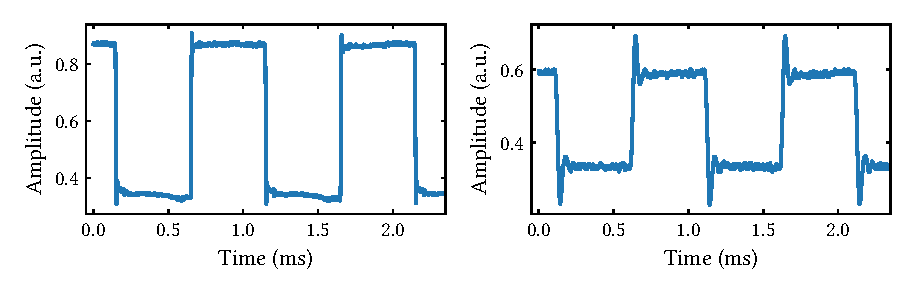
\includegraphics{figures/eom_example_traces_155.pdf}
}
\caption{Example traces of light passing through an \ac{eom} and filtered using a polarizing beam splitter. The materials used are \ac{rtp} (left) and \ac{bbo} (right). The absolute value of the amplitude depends on the input power of the laser and was different for both measurements.}
\end{figure}

Stress on the crystal causes the amplitude of the laser on the output of the \ac{eom} to be inconsistent when driving the pockels cell for long times (\~{}$\SI{1}{\second}$) and high repetition rates (\~{}\SI{}{MHz}). This effect can be reduced by alternating the voltage applied to the crystal, which results in Figure \ref{fig:eom_amp_time}, however the effect can only be seen on the \ac{rtp} crystal and not on the \ac{bbo}. With this information, it is clear that the \ac{rtp} crystal should be driven with frequencies up to $\SI{1.2}{\mega \hertz}$ or in the range $1.5$ to $\SI{1.7}{\mega \hertz}$. The amplitude was extracted from the traces by fitting a fourier series.

\begin{figure}[t]
\label{fig:eom_amp_time}
\centering{
	\setlength{\figureheight}{2in}
	\setlength{\figurewidth}{\textwidth-1.2em}
	%% This file was created by tikzplotlib v0.9.4.
\begin{tikzpicture}

\definecolor{color0}{rgb}{0.12156862745098,0.466666666666667,0.705882352941177}
\definecolor{color1}{rgb}{1,0.498039215686275,0.0549019607843137}

\begin{axis}[
height=\figureheight,
minor xtick={},
minor ytick={},
scaled y ticks=false,
tick align=inside,
tick pos=both,
width=\figurewidth,
x grid style={white!69.0196078431373!black},
xlabel={Frequency (MHz)},
xmin=0.95, xmax=2.05,
xtick style={color=black},
xtick={0.8,1,1.2,1.4,1.6,1.8,2,2.2},
xticklabels={0.8,1.0,1.2,1.4,1.6,1.8,2.0,2.2},
y grid style={white!69.0196078431373!black},
y tick label style={/pgf/number format/fixed},
ylabel style={align=center},
ylabel={Normalized Amplitude},
ymin=-0.05, ymax=1.05,
ytick style={color=black},
ytick={-0.5,0,0.5,1,1.5},
yticklabels={−0.25,0.00,0.25,0.50,0.75}
]
\addplot [line width=1.5pt, color0]
table {%
1 0.958240471323278
1.00150075037519 0.955765591308188
1.00300150075038 0.955620537636412
1.00450225112556 0.957828600953296
1.00600300150075 0.960057446813028
1.00750375187594 0.959368323428149
1.00900450225113 0.95973152643672
1.01050525262631 0.958514421315365
1.0120060030015 0.955752982242716
1.01350675337669 0.959026147379477
1.01500750375188 0.957330048117813
1.01650825412706 0.955517438464046
1.01800900450225 0.958426138172206
1.01950975487744 0.960184432072817
1.02101050525263 0.954662718807043
1.02251125562781 0.958016651327419
1.024012006003 0.956794640653859
1.02551275637819 0.95670292248929
1.02701350675338 0.958396413490181
1.02851425712856 0.958777565962598
1.03001500750375 0.960395087416408
1.03151575787894 0.957947813665374
1.03301650825413 0.958031323565406
1.03451725862931 0.956163061821321
1.0360180090045 0.955926791211139
1.03751875937969 0.958272986056345
1.03901950975488 0.95505170622911
1.04052026013006 0.960819052702023
1.04202101050525 0.959326686521515
1.04352176088044 0.95976386574891
1.04502251125563 0.95656579400304
1.04652326163082 0.956506015665391
1.048024012006 0.955308766914294
1.04952476238119 0.959407919193947
1.05102551275638 0.960041499202804
1.05252626313157 0.962095161245471
1.05402701350675 0.960342333824507
1.05552776388194 0.957533571400656
1.05702851425713 0.957045323639139
1.05852926463232 0.9591802590765
1.0600300150075 0.960390880039044
1.06153076538269 0.959288110059708
1.06303151575788 0.959103380240884
1.06453226613307 0.953323553195595
1.06603301650825 0.955807451034018
1.06753376688344 0.958611700494804
1.06903451725863 0.957475113023956
1.07053526763382 0.95712458529806
1.072036018009 0.952163214985017
1.07353676838419 0.946277536130315
1.07503751875938 0.949171437518897
1.07653826913457 0.948656191005031
1.07803901950975 0.950590461355813
1.07953976988494 0.95302736113175
1.08104052026013 0.94981283982246
1.08254127063532 0.94967129521469
1.08404202101051 0.951560196282567
1.08554277138569 0.947497202737719
1.08704352176088 0.948292267303944
1.08854427213607 0.953492454767396
1.09004502251126 0.951033810050398
1.09154577288644 0.950733900735913
1.09304652326163 0.954660445426587
1.09454727363682 0.952588845485224
1.09604802401201 0.950605670921092
1.09754877438719 0.950589901252007
1.09904952476238 0.953635044910631
1.10055027513757 0.956073323957815
1.10205102551276 0.952880876144935
1.10355177588794 0.95136381505861
1.10505252626313 0.955331200231453
1.10655327663832 0.955772522423534
1.10805402701351 0.954588983710219
1.10955477738869 0.955208122295766
1.11105552776388 0.954974040511398
1.11255627813907 0.95533889688093
1.11405702851426 0.955810346033623
1.11555777888944 0.954486448243219
1.11705852926463 0.957977072857676
1.11855927963982 0.957009784362125
1.12006003001501 0.957671084729791
1.1215607803902 0.956120697539119
1.12306153076538 0.954364877548246
1.12456228114057 0.956276589227362
1.12606303151576 0.956856738236108
1.12756378189095 0.957991309705294
1.12906453226613 0.958389242089793
1.13056528264132 0.961176891030128
1.13206603301651 0.957751463767166
1.1335667833917 0.957958584409856
1.13506753376688 0.953271746107741
1.13656828414207 0.956289672764335
1.13806903451726 0.95944429298193
1.13956978489245 0.958053851023294
1.14107053526763 0.957840229352852
1.14257128564282 0.958198852288613
1.14407203601801 0.956483456269557
1.1455727863932 0.954099847810489
1.14707353676838 0.954562704188519
1.14857428714357 0.958692727512999
1.15007503751876 0.956410143134529
1.15157578789395 0.957657648149217
1.15307653826913 0.956547981849511
1.15457728864432 0.958266395851038
1.15607803901951 0.957129382470627
1.1575787893947 0.957728395804048
1.15907953976988 0.958627278470489
1.16058029014507 0.957657172316722
1.16208104052026 0.958501280060365
1.16358179089545 0.959253153993166
1.16508254127064 0.954479931414179
1.16658329164582 0.958137350018109
1.16808404202101 0.961062253868861
1.1695847923962 0.959097973263758
1.17108554277139 0.958039949668083
1.17258629314657 0.957680034998663
1.17408704352176 0.952280669679428
1.17558779389695 0.958389198358536
1.17708854427214 0.960630696934947
1.17858929464732 0.962576619772016
1.18009004502251 0.959731064035448
1.1815907953977 0.962578459193511
1.18309154577289 0.958544333871073
1.18459229614807 0.958373426654759
1.18609304652326 0.957629146927843
1.18759379689845 0.959584391626377
1.18909454727364 0.958749226461126
1.19059529764882 0.959207070091998
1.19209604802401 0.95989543903368
1.1935967983992 0.961934385675639
1.19509754877439 0.958192531512004
1.19659829914957 0.959751095065762
1.19809904952476 0.960051806117197
1.19959979989995 0.958903053903419
1.20110055027514 0.955628437309198
1.20260130065033 0.957119298503051
1.20410205102551 0.958244498426101
1.2056028014007 0.956584959012953
1.20710355177589 0.957344746487443
1.20860430215108 0.95768714594959
1.21010505252626 0.958072798078421
1.21160580290145 0.956623191320148
1.21310655327664 0.954999299973142
1.21460730365183 0.95358159630967
1.21610805402701 0.956368787927726
1.2176088044022 0.959661381757854
1.21910955477739 0.961160175498501
1.22061030515258 0.957436915242769
1.22211105552776 0.95778347553089
1.22361180590295 0.955564190303698
1.22511255627814 0.956049878384048
1.22661330665333 0.957914339275964
1.22811405702851 0.962212982193289
1.2296148074037 0.962027724779185
1.23111555777889 0.95912236113418
1.23261630815408 0.960104359660653
1.23411705852926 0.957928486854394
1.23561780890445 0.958254466997473
1.23711855927964 0.960080482343446
1.23861930965483 0.961406140499506
1.24012006003002 0.961335550159664
1.2416208104052 0.961442835343715
1.24312156078039 0.962362636689688
1.24462231115558 0.960795793663401
1.24612306153077 0.961650062388667
1.24762381190595 0.964338435644848
1.24912456228114 0.963185505489029
1.25062531265633 0.960540447839679
1.25212606303152 0.961156260966209
1.2536268134067 0.962609595170174
1.25512756378189 0.963182097882494
1.25662831415708 0.960715501104284
1.25812906453227 0.96239829298671
1.25962981490745 0.959605499852459
1.26113056528264 0.959805522464988
1.26263131565783 0.961463234079288
1.26413206603302 0.960663753574888
1.2656328164082 0.962973275813607
1.26713356678339 0.963290504535161
1.26863431715858 0.964067749651528
1.27013506753377 0.962768609978102
1.27163581790895 0.962032074797884
1.27313656828414 0.962159288082527
1.27463731865933 0.961315857572643
1.27613806903452 0.959632331053591
1.2776388194097 0.965045026781337
1.27913956978489 0.965489490039274
1.28064032016008 0.963041516981085
1.28214107053527 0.962760921659839
1.28364182091046 0.958783219042116
1.28514257128564 0.956806426778895
1.28664332166083 0.961272700023716
1.28814407203602 0.963483274658152
1.28964482241121 0.960101349370105
1.29114557278639 0.963041566088618
1.29264632316158 0.962197027825909
1.29414707353677 0.957666906132081
1.29564782391196 0.955889834304999
1.29714857428714 0.958587609982291
1.29864932466233 0.959524842114937
1.30015007503752 0.96214740642688
1.30165082541271 0.961492015830745
1.30315157578789 0.961430465687755
1.30465232616308 0.95985819063399
1.30615307653827 0.960090913897877
1.30765382691346 0.960375844331188
1.30915457728864 0.960109805015276
1.31065532766383 0.959085540706062
1.31215607803902 0.9569463603454
1.31365682841421 0.9579875593595
1.31515757878939 0.95611309300985
1.31665832916458 0.960491358134389
1.31815907953977 0.95872128728402
1.31965982991496 0.955977555934172
1.32116058029015 0.958420576375087
1.32266133066533 0.957716812759288
1.32416208104052 0.957653024372643
1.32566283141571 0.95832384996544
1.3271635817909 0.957258009179264
1.32866433216608 0.961863870117037
1.33016508254127 0.956297786430208
1.33166583291646 0.957938412598544
1.33316658329165 0.95612214422965
1.33466733366683 0.956387418251376
1.33616808404202 0.958510151957272
1.33766883441721 0.956674669730271
1.3391695847924 0.958546829715016
1.34067033516758 0.958088160393557
1.34217108554277 0.959642365940971
1.34367183591796 0.956764404422306
1.34517258629315 0.955471238059799
1.34667333666833 0.956593056180324
1.34817408704352 0.957225551293764
1.34967483741871 0.958430846998295
1.3511755877939 0.957182469951054
1.35267633816908 0.959033135417604
1.35417708854427 0.957172501680379
1.35567783891946 0.953821687695856
1.35717858929465 0.955945938027054
1.35867933966983 0.955772774384042
1.36018009004502 0.954206314700641
1.36168084042021 0.947928941083229
1.3631815907954 0.950364385855713
1.36468234117059 0.943945314088795
1.36618309154577 0.946026004521651
1.36768384192096 0.946444065763184
1.36918459229615 0.948300281655659
1.37068534267134 0.947472285027374
1.37218609304652 0.945797086812219
1.37368684342171 0.946190842731405
1.3751875937969 0.950208072194968
1.37668834417209 0.945957627255254
1.37818909454727 0.9500503612302
1.37968984492246 0.953496310358774
1.38119059529765 0.947551644686542
1.38269134567284 0.948940501056929
1.38419209604802 0.946486025407657
1.38569284642321 0.948471267937629
1.3871935967984 0.948269822920463
1.38869434717359 0.951443393318912
1.39019509754877 0.952586121570915
1.39169584792396 0.953770132477949
1.39319659829915 0.952490808219111
1.39469734867434 0.94948760728426
1.39619809904952 0.953849403328844
1.39769884942471 0.955550001388454
1.3991995997999 0.956871208879841
1.40070035017509 0.958575920687336
1.40220110055028 0.956872617491259
1.40370185092546 0.955912129191621
1.40520260130065 0.9572639097938
1.40670335167584 0.957065816362467
1.40820410205103 0.956459636487517
1.40970485242621 0.962231302654412
1.4112056028014 0.964475531265138
1.41270635317659 0.967007482884559
1.41420710355178 0.966360777644639
1.41570785392696 0.967952132814654
1.41720860430215 0.969136112335762
1.41870935467734 0.973200131152582
1.42021010505253 0.972649782528349
1.42171085542771 0.976632744213351
1.4232116058029 0.979069938736645
1.42471235617809 0.979046443468039
1.42621310655328 0.982522949054918
1.42771385692846 0.985903499164381
1.42921460730365 0.986550008150956
1.43071535767884 0.984116777042617
1.43221610805403 0.981710005367905
1.43371685842921 0.983203743188068
1.4352176088044 0.982672700419196
1.43671835917959 0.985848484768294
1.43821910955478 0.985887003084258
1.43971985992996 0.986685464673487
1.44122061030515 0.986511748438456
1.44272136068034 0.988519686926714
1.44422211105553 0.986595920148964
1.44572286143072 0.988575389019042
1.4472236118059 0.99223149423754
1.44872436218109 0.990482961004897
1.45022511255628 0.993030508205783
1.45172586293147 0.992867755539669
1.45322661330665 0.991973576332518
1.45472736368184 0.993130362708759
1.45622811405703 0.993570902991989
1.45772886443222 0.991406769194645
1.4592296148074 0.993541328296636
1.46073036518259 0.992447970693333
1.46223111555778 0.991777585813055
1.46373186593297 0.992910829122715
1.46523261630815 0.990141709586069
1.46673336668334 0.996490133472951
1.46823411705853 0.993793567196568
1.46973486743372 0.993975759061437
1.4712356178089 0.990760536515173
1.47273636818409 0.993434517102197
1.47423711855928 0.99289138585418
1.47573786893447 0.992671538950003
1.47723861930965 0.995148596857487
1.47873936968484 0.994834128642621
1.48024012006003 0.992557123565414
1.48174087043522 0.990966484801331
1.48324162081041 0.986709826611075
1.48474237118559 0.986202516001605
1.48624312156078 0.992434236930288
1.48774387193597 0.990935890404871
1.48924462231116 0.991597080075278
1.49074537268634 0.990332267594491
1.49224612306153 0.990528329630221
1.49374687343672 0.983983867435916
1.49524762381191 0.984055294234496
1.49674837418709 0.987046901759671
1.49824912456228 0.985227123886383
1.49974987493747 0.984950118247705
1.50125062531266 0.983554141503584
1.50275137568784 0.988903688962851
1.50425212606303 0.987908561232092
1.50575287643822 0.986341633213486
1.50725362681341 0.985817989471691
1.50875437718859 0.984329039049079
1.51025512756378 0.984039899053588
1.51175587793897 0.980797323741189
1.51325662831416 0.984920726566432
1.51475737868934 0.988387553183224
1.51625812906453 0.990727096830401
1.51775887943972 0.987615583712499
1.51925962981491 0.98849995620113
1.5207603801901 0.985477848887382
1.52226113056528 0.984773131620957
1.52376188094047 0.984956455521953
1.52526263131566 0.983814528111015
1.52676338169085 0.987561500748046
1.52826413206603 0.988246278716138
1.52976488244122 0.9904443961726
1.53126563281641 0.99127853973567
1.5327663831916 0.988998470406475
1.53426713356678 0.990083282493234
1.53576788394197 0.994369210791513
1.53726863431716 0.992619476982356
1.53876938469235 0.991015637903889
1.54027013506753 0.992285297017221
1.54177088544272 0.994098982779349
1.54327163581791 0.99035062551897
1.5447723861931 0.989379013962044
1.54627313656828 0.993310328204182
1.54777388694347 0.993275437370949
1.54927463731866 0.994363777432792
1.55077538769385 0.994250417882373
1.55227613806903 0.99278444384898
1.55377688844422 0.995732364573626
1.55527763881941 0.99359212566352
1.5567783891946 0.991901723559053
1.55827913956978 0.993889892834922
1.55977988994497 0.990493289886479
1.56128064032016 0.993969635878333
1.56278139069535 0.991296387426684
1.56428214107054 0.993083108098569
1.56578289144572 0.995772104621653
1.56728364182091 0.990401706508612
1.5687843921961 0.989657798171885
1.57028514257129 0.989986878225522
1.57178589294647 0.991666505587868
1.57328664332166 0.991071810451643
1.57478739369685 0.992223717750986
1.57628814407204 0.992549585159107
1.57778889444722 0.990013428549714
1.57928964482241 0.991047133425429
1.5807903951976 0.99050473153248
1.58229114557279 0.989318097686439
1.58379189594797 0.989273362791115
1.58529264632316 0.989755700151416
1.58679339669835 0.990023368705132
1.58829414707354 0.993213724730029
1.58979489744872 0.991655209783005
1.59129564782391 0.992961675655285
1.5927963981991 0.990920435841857
1.59429714857429 0.988655599433433
1.59579789894947 0.990049787131169
1.59729864932466 0.992187528822471
1.59879939969985 0.992668270586837
1.60030015007504 0.990006746239323
1.60180090045023 0.99149341229318
1.60330165082541 0.993434857951524
1.6048024012006 0.989969360795772
1.60630315157579 0.993995584222323
1.60780390195098 0.993208356770707
1.60930465232616 0.991625669940365
1.61080540270135 0.992188752745079
1.61230615307654 0.993857819864978
1.61380690345173 0.992056827268176
1.61530765382691 0.993192173298398
1.6168084042021 0.991838747576879
1.61830915457729 0.992656107680591
1.61980990495248 0.992310649103638
1.62131065532766 0.991234780869187
1.62281140570285 0.990188597702586
1.62431215607804 0.991068258475609
1.62581290645323 0.991800810878989
1.62731365682841 0.993812383002499
1.6288144072036 0.993723345731096
1.63031515757879 0.993561794553363
1.63181590795398 0.992466763132866
1.63331665832916 0.990707773412822
1.63481740870435 0.988979865764416
1.63631815907954 0.992521594377859
1.63781890945473 0.993645387297109
1.63931965982992 0.99454633434849
1.6408204102051 0.993176309646147
1.64232116058029 0.993146089806076
1.64382191095548 0.989623831163586
1.64532266133067 0.992017420393791
1.64682341170585 0.992402388732625
1.64832416208104 0.993118390394842
1.64982491245623 0.991798124216472
1.65132566283142 0.993130933841988
1.6528264132066 0.990642621254708
1.65432716358179 0.988569681120131
1.65582791395698 0.99052561434468
1.65732866433217 0.990243669764503
1.65882941470735 0.991531108094546
1.66033016508254 0.990741316328116
1.66183091545773 0.991546556117336
1.66333166583292 0.990913461501632
1.6648324162081 0.99091878479455
1.66633316658329 0.992187813941301
1.66783391695848 0.989528243669761
1.66933466733367 0.989674054650117
1.67083541770885 0.991045179257104
1.67233616808404 0.993784556325578
1.67383691845923 0.991686731938808
1.67533766883442 0.992384061456807
1.6768384192096 0.993961301148348
1.67833916958479 0.994910763725002
1.67983991995998 0.991823269217379
1.68134067033517 0.990551242000176
1.68284142071036 0.987716547309656
1.68434217108554 0.988031296125614
1.68584292146073 0.989176159731423
1.68734367183592 0.989322349250339
1.68884442221111 0.992472136819396
1.69034517258629 0.988281697615522
1.69184592296148 0.987333416458082
1.69334667333667 0.987806058992647
1.69484742371186 0.986714186428858
1.69634817408704 0.985358839750947
1.69784892446223 0.989069175546103
1.69934967483742 0.986222791398285
1.70085042521261 0.988609160693915
1.70235117558779 0.990861535217178
1.70385192596298 0.987439336070248
1.70535267633817 0.989357565379946
1.70685342671336 0.989473999668822
1.70835417708854 0.987571623086012
1.70985492746373 0.988004681713645
1.71135567783892 0.987529113088418
1.71285642821411 0.986038017008698
1.71435717858929 0.988675488346587
1.71585792896448 0.988771267922166
1.71735867933967 0.989729491866053
1.71885942971486 0.985587199779856
1.72036018009004 0.990017672176808
1.72186093046523 0.989616207359506
1.72336168084042 0.987190687150512
1.72486243121561 0.988534284750376
1.7263631815908 0.989932822349606
1.72786393196598 0.992437834512839
1.72936468234117 0.9862635627999
1.73086543271636 0.987599572946799
1.73236618309155 0.989514961623071
1.73386693346673 0.986403804106017
1.73536768384192 0.989220574191568
1.73686843421711 0.989474903526472
1.7383691845923 0.988704525396514
1.73986993496748 0.989507788622025
1.74137068534267 0.987890743026496
1.74287143571786 0.985234818501075
1.74437218609305 0.987014020571414
1.74587293646823 0.985811124601845
1.74737368684342 0.990443751317789
1.74887443721861 0.987022857165859
1.7503751875938 0.989605250196685
1.75187593796898 0.988998719016148
1.75337668834417 0.987638465035079
1.75487743871936 0.98670135549284
1.75637818909455 0.987379147239732
1.75787893946973 0.988740571030031
1.75937968984492 0.990153376343465
1.76088044022011 0.986757183863408
1.7623811905953 0.988944785801751
1.76388194097049 0.987147090573738
1.76538269134567 0.99145815331793
1.76688344172086 0.988606089778493
1.76838419209605 0.986640604468314
1.76988494247124 0.987865306132559
1.77138569284642 0.985823588067675
1.77288644322161 0.987532067195985
1.7743871935968 0.985685577343536
1.77588794397199 0.993161783876756
1.77738869434717 0.991185372304302
1.77888944472236 0.990391189705593
1.78039019509755 0.98861879173927
1.78189094547274 0.986965536633559
1.78339169584792 0.988488654778697
1.78489244622311 0.98793528876268
1.7863931965983 0.989626983631708
1.78789394697349 0.989111592782198
1.78939469734867 0.990455018837756
1.79089544772386 0.990158234332554
1.79239619809905 0.989403368087167
1.79389694847424 0.987168152227972
1.79539769884942 0.989473723774089
1.79689844922461 0.989103351605557
1.7983991995998 0.989499997376921
1.79989994997499 0.988820871406954
1.80140070035018 0.990017514164028
1.80290145072536 0.989269542050518
1.80440220110055 0.98807200694807
1.80590295147574 0.98846781835136
1.80740370185093 0.989774623821575
1.80890445222611 0.991132759321054
1.8104052026013 0.992358970655786
1.81190595297649 0.993543170240029
1.81340670335168 0.991902109538031
1.81490745372686 0.991993535596188
1.81640820410205 0.992391008200563
1.81790895447724 0.992050286365176
1.81940970485243 0.991080570931894
1.82091045522761 0.988241609196094
1.8224112056028 0.990260617734378
1.82391195597799 0.986822492944435
1.82541270635318 0.99051863017716
1.82691345672836 0.994361878070481
1.82841420710355 0.99101031557246
1.82991495747874 0.989096502920396
1.83141570785393 0.987801845470019
1.83291645822911 0.988987155653354
1.8344172086043 0.989670221778665
1.83591795897949 0.991632957298819
1.83741870935468 0.990515669659922
1.83891945972987 0.991726421242308
1.84042021010505 0.989990370283697
1.84192096048024 0.990689934140664
1.84342171085543 0.989166323038494
1.84492246123062 0.989715805260962
1.8464232116058 0.991476875418131
1.84792396198099 0.991443523749963
1.84942471235618 0.990505441374355
1.85092546273137 0.991803433087078
1.85242621310655 0.992164897841376
1.85392696348174 0.98913469397926
1.85542771385693 0.989289872176304
1.85692846423212 0.992038341063532
1.8584292146073 0.992300539640784
1.85992996498249 0.991907011969771
1.86143071535768 0.991109597573001
1.86293146573287 0.99128146149641
1.86443221610805 0.991297854181849
1.86593296648324 0.992186853608812
1.86743371685843 0.993232421759511
1.86893446723362 0.990526082426639
1.8704352176088 0.98954470610329
1.87193596798399 0.990218493899296
1.87343671835918 0.991260232871402
1.87493746873437 0.993875686400055
1.87643821910955 0.994551413037214
1.87793896948474 0.994768072631052
1.87943971985993 0.992066330576104
1.88094047023512 0.989808259157793
1.88244122061031 0.989762630581066
1.88394197098549 0.9910037778338
1.88544272136068 0.992162489657275
1.88694347173587 0.992096880758961
1.88844422211106 0.99385121817957
1.88994497248624 0.992729177154223
1.89144572286143 0.993282155631064
1.89294647323662 0.991137924754717
1.89444722361181 0.992584939285654
1.89594797398699 0.992517150870396
1.89744872436218 0.995666245372067
1.89894947473737 0.992885105219143
1.90045022511256 0.996243427342429
1.90195097548774 0.992511855690603
1.90345172586293 0.990671683010141
1.90495247623812 0.993967029334798
1.90645322661331 0.99131248559687
1.90795397698849 0.990794501863476
1.90945472736368 0.991229524726672
1.91095547773887 0.987714997944258
1.91245622811406 0.988693151746873
1.91395697848924 0.99094066262149
1.91545772886443 0.990793821461196
1.91695847923962 0.991925309729863
1.91845922961481 0.994522808768912
1.91995997998999 0.994062450808532
1.92146073036518 0.995803472256004
1.92296148074037 0.993417553498957
1.92446223111556 0.994632714007127
1.92596298149075 0.998057456033245
1.92746373186593 0.996688863782786
1.92896448224112 0.997499360718917
1.93046523261631 0.995856506166173
1.9319659829915 0.995068798839263
1.93346673336668 0.994084965277339
1.93496748374187 0.999138616034683
1.93646823411706 0.997963892786656
1.93796898449225 0.995535139548336
1.93946973486743 0.99725340801629
1.94097048524262 0.995547610713072
1.94247123561781 0.995898032703005
1.943971985993 0.994897580668802
1.94547273636818 0.994170439436946
1.94697348674337 0.997196837541095
1.94847423711856 0.996607279482769
1.94997498749375 0.999020634622417
1.95147573786893 0.997984933055679
1.95297648824412 0.996352996216267
1.95447723861931 0.996090309084277
1.9559779889945 0.99750199313539
1.95747873936968 0.996219632786986
1.95897948974487 0.994248897487255
1.96048024012006 0.995737050884722
1.96198099049525 0.994353850215428
1.96348174087044 0.995232421224981
1.96498249124562 0.995260767727472
1.96648324162081 0.996778323406204
1.967983991996 0.995551313018955
1.96948474237119 0.995070637538261
1.97098549274637 0.997447641273714
1.97248624312156 0.995418494668022
1.97398699349675 0.998135493735855
1.97548774387194 0.996117364222715
1.97698849424712 1
1.97848924462231 0.995723892919332
1.9799899949975 0.995987409796398
1.98149074537269 0.996536027996938
1.98299149574787 0.995718812461595
1.98449224612306 0.99827548498243
1.98599299649825 0.998300865400035
1.98749374687344 0.99549734164138
1.98899449724862 0.998375792182429
1.99049524762381 0.998213715956604
1.991995997999 0.998644041407232
1.99349674837419 0.995064728145437
1.99499749874937 0.998729582407633
1.99649824912456 0.995691058325329
1.99799899949975 0.997729817549313
1.99949974987494 0.998318544970013
};
\addplot [line width=1.5pt, color1]
table {%
1 0.990147522249168
1.00200400801603 0.996449250342955
1.00400801603206 1
1.0060120240481 0.9963419962043
1.00801603206413 0.988784977607459
1.01002004008016 0.980377322351208
1.01202404809619 0.974915985705703
1.01402805611222 0.967795520260504
1.01603206412826 0.970933375870833
1.01803607214429 0.973807283028414
1.02004008016032 0.977437369528237
1.02204408817635 0.976173268800942
1.02404809619238 0.972605113172264
1.02605210420842 0.974057022805923
1.02805611222445 0.976222416906075
1.03006012024048 0.978243551923738
1.03206412825651 0.977373109318136
1.03406813627255 0.973573550719129
1.03607214428858 0.964712775672747
1.03807615230461 0.956161333998036
1.04008016032064 0.934348951680696
1.04208416833667 0.91177915371219
1.04408817635271 0.909922460683172
1.04609218436874 0.90746325473495
1.04809619238477 0.904622874181154
1.0501002004008 0.894689952649373
1.05210420841683 0.889925334656508
1.05410821643287 0.903019231383528
1.0561122244489 0.917011018066523
1.05811623246493 0.91974099343212
1.06012024048096 0.924971027654564
1.06212424849699 0.916205553422628
1.06412825651303 0.904728948993425
1.06613226452906 0.900693365866258
1.06813627254509 0.903466819453237
1.07014028056112 0.898393840189015
1.07214428857715 0.887114074277531
1.07414829659319 0.881777650745441
1.07615230460922 0.886922818723089
1.07815631262525 0.894338867208478
1.08016032064128 0.906320982658451
1.08216432865731 0.911276905433844
1.08416833667335 0.914898614838391
1.08617234468938 0.913739517762913
1.08817635270541 0.917380036117783
1.09018036072144 0.918226265428739
1.09218436873748 0.925693597841367
1.09418837675351 0.928724689372379
1.09619238476954 0.92882735228527
1.09819639278557 0.930270621931059
1.1002004008016 0.932014646270108
1.10220440881764 0.928902212971339
1.10420841683367 0.930286187713311
1.1062124248497 0.931473521744415
1.10821643286573 0.933899709954273
1.11022044088176 0.93536994767931
1.1122244488978 0.93987338566696
1.11422845691383 0.946606382936369
1.11623246492986 0.955821374499782
1.11823647294589 0.960972196951436
1.12024048096192 0.970306810784943
1.12224448897796 0.978628055435876
1.12424849699399 0.983176179823504
1.12625250501002 0.990113457820024
1.12825651302605 0.994696458939781
1.13026052104208 0.991588341086651
1.13226452905812 0.99320825578575
1.13426853707415 0.987287284711055
1.13627254509018 0.982665312920143
1.13827655310621 0.975266382570401
1.14028056112224 0.960237099610991
1.14228456913828 0.956485255019735
1.14428857715431 0.961944846813158
1.14629258517034 0.965367987320258
1.14829659318637 0.967590559790251
1.1503006012024 0.968771128746347
1.15230460921844 0.968417573218284
1.15430861723447 0.971329466211875
1.1563126252505 0.974885802191193
1.15831663326653 0.97778092328156
1.16032064128257 0.980006725851132
1.1623246492986 0.984025534233995
1.16432865731463 0.981168445752826
1.16633266533066 0.986217389021952
1.16833667334669 0.990800898510473
1.17034068136273 0.991436596124322
1.17234468937876 0.991964682218703
1.17434869739479 0.992056879945657
1.17635270541082 0.990752566956474
1.17835671342685 0.990742879528281
1.18036072144289 0.982637915602529
1.18236472945892 0.969185524605911
1.18436873747495 0.958581894316526
1.18637274549098 0.95442273383677
1.18837675350701 0.949738199489497
1.19038076152305 0.944185235319689
1.19238476953908 0.938651704715228
1.19438877755511 0.934774542307002
1.19639278557114 0.929027077313301
1.19839679358717 0.922922130085649
1.20040080160321 0.922676080722958
1.20240480961924 0.935078428313042
1.20440881763527 0.942296467728409
1.2064128256513 0.947631909221674
1.20841683366733 0.951268047196897
1.21042084168337 0.953509542081908
1.2124248496994 0.955890027435991
1.21442885771543 0.954931134481887
1.21643286573146 0.950721784380327
1.21843687374749 0.942891167365624
1.22044088176353 0.933158497307502
1.22244488977956 0.918317351727589
1.22444889779559 0.910525193822782
1.22645290581162 0.906345556709246
1.22845691382766 0.907996797176429
1.23046092184369 0.912328509096334
1.23246492985972 0.913972865721103
1.23446893787575 0.910332353605415
1.23647294589178 0.89340234592896
1.23847695390782 0.865940331691956
1.24048096192385 0.859778480175663
1.24248496993988 0.849900288412112
1.24448897795591 0.841286524781878
1.24649298597194 0.829242084818544
1.24849699398798 0.820813125646135
1.25050100200401 0.817703503226655
1.25250501002004 0.801065230577676
1.25450901803607 0.774298150788868
1.2565130260521 0.740453496437832
1.25851703406814 0.739954065191943
1.26052104208417 0.76767533931526
1.2625250501002 0.791017602344053
1.26452905811623 0.778210564475428
1.26653306613226 0.771581372907181
1.2685370741483 0.762572688193442
1.27054108216433 0.75013613220831
1.27254509018036 0.758522945219106
1.27454909819639 0.788287847089672
1.27655310621242 0.81756306493414
1.27855711422846 0.840154742533852
1.28056112224449 0.858278127024254
1.28256513026052 0.852683785489505
1.28456913827655 0.847977161563038
1.28657314629259 0.850513859874316
1.28857715430862 0.860042269301684
1.29058116232465 0.870581622668319
1.29258517034068 0.877856486579903
1.29458917835671 0.875979628136906
1.29659318637275 0.863840417538519
1.29859719438878 0.836729652883377
1.30060120240481 0.801306391636757
1.30260521042084 0.762509918091199
1.30460921843687 0.730006136659631
1.30661322645291 0.728001598736697
1.30861723446894 0.736030586415814
1.31062124248497 0.742470552940228
1.312625250501 0.749113799947671
1.31462925851703 0.759293008523048
1.31663326653307 0.772488286503453
1.3186372745491 0.777783381402752
1.32064128256513 0.768202761355657
1.32264529058116 0.767083929092863
1.32464929859719 0.756776407361932
1.32665330661323 0.734596921476218
1.32865731462926 0.70621156766449
1.33066132264529 0.658515826160761
1.33266533066132 0.584512115112871
1.33466933867735 0.451560407871815
1.33667334669339 0.268801347469669
1.33867735470942 0.1013779676603
1.34068136272545 0.0129681528116031
1.34268537074148 0.00535405274501119
1.34468937875751 0.0248866288159281
1.34669338677355 0.0710103357231658
1.34869739478958 0.120421948269728
1.35070140280561 0.177259049051772
1.35270541082164 0.232553624031913
1.35470941883768 0.289235273107845
1.35671342685371 0.33657674608237
1.35871743486974 0.380751255940646
1.36072144288577 0.41963856191516
1.3627254509018 0.452494293591471
1.36472945891784 0.453663786635154
1.36673346693387 0.447677849601862
1.3687374749499 0.439902936496915
1.37074148296593 0.435169329921563
1.37274549098196 0.426723966753527
1.374749498998 0.409529577073103
1.37675350701403 0.384249911201248
1.37875751503006 0.364662930017059
1.38076152304609 0.379935573008099
1.38276553106212 0.417923116634041
1.38476953907816 0.466802900908619
1.38677354709419 0.514627437920525
1.38877755511022 0.550233601098406
1.39078156312625 0.577830605665268
1.39278557114228 0.618404237161702
1.39478957915832 0.666337675529325
1.39679358717435 0.714776094474533
1.39879759519038 0.731576695007852
1.40080160320641 0.728695151297767
1.40280561122244 0.718581599848213
1.40480961923848 0.707713128867219
1.40681362725451 0.682929394587653
1.40881763527054 0.650632950688319
1.41082164328657 0.604392589802555
1.41282565130261 0.555719346569591
1.41482965931864 0.522738884530519
1.41683366733467 0.492954545629567
1.4188376753507 0.483430738270722
1.42084168336673 0.481803931684536
1.42284569138277 0.466504289008159
1.4248496993988 0.448438108584691
1.42685370741483 0.423732799525181
1.42885771543086 0.409284505603413
1.43086172344689 0.41068390859983
1.43286573146293 0.423369543218647
1.43486973947896 0.451973782893847
1.43687374749499 0.502907481274595
1.43887775551102 0.570343534701867
1.44088176352705 0.621245228335099
1.44288577154309 0.67035227261384
1.44488977955912 0.697581370990058
1.44689378757515 0.725155342377079
1.44889779559118 0.749573832926115
1.45090180360721 0.781453630117277
1.45290581162325 0.807411081409043
1.45490981963928 0.828769898198832
1.45691382765531 0.853021118580954
1.45891783567134 0.874130054410369
1.46092184368737 0.887268118233096
1.46292585170341 0.895439745342307
1.46492985971944 0.89865325107728
1.46693386773547 0.900682152620288
1.4689378757515 0.913208783228331
1.47094188376753 0.920556831364899
1.47294589178357 0.933831608325496
1.4749498997996 0.953901159656848
1.47695390781563 0.962187785787258
1.47895791583166 0.962660571902397
1.4809619238477 0.956822861381727
1.48296593186373 0.951286237530228
1.48496993987976 0.954113464530224
1.48697394789579 0.955667386038112
1.48897795591182 0.9620479196171
1.49098196392786 0.958983237106774
1.49298597194389 0.964482318954497
1.49498997995992 0.964718791377672
1.49699398797595 0.970971764357054
1.49899799599198 0.963911079252774
1.50100200400802 0.960189322260788
1.50300601202405 0.951526658241931
1.50501002004008 0.946413946639297
1.50701402805611 0.944226713135448
1.50901803607214 0.946212493434078
1.51102204408818 0.94361089018374
1.51302605210421 0.941759075612268
1.51503006012024 0.938934272795696
1.51703406813627 0.922356835443548
1.5190380761523 0.920126452695828
1.52104208416834 0.912802316898804
1.52304609218437 0.910326831856641
1.5250501002004 0.900646715467071
1.52705410821643 0.914683346800804
1.52905811623247 0.911438392305171
1.5310621242485 0.912515132833622
1.53306613226453 0.912552086881341
1.53507014028056 0.919593564854721
1.53707414829659 0.928978459781314
1.53907815631263 0.923024188710286
1.54108216432866 0.933691871253146
1.54308617234469 0.940488288877388
1.54509018036072 0.942430945217806
1.54709418837675 0.95313965555286
1.54909819639279 0.954562377867999
1.55110220440882 0.955867373730627
1.55310621242485 0.955652833016935
1.55511022044088 0.958146767095367
1.55711422845691 0.956376442220833
1.55911823647295 0.960313400172248
1.56112224448898 0.951010574779829
1.56312625250501 0.952584941471386
1.56513026052104 0.945455367079903
1.56713426853707 0.942151144143276
1.56913827655311 0.941928465735052
1.57114228456914 0.929156634192575
1.57314629258517 0.925163007080831
1.5751503006012 0.920241565858794
1.57715430861723 0.892679143478064
1.57915831663327 0.861437570119223
1.5811623246493 0.823742678293933
1.58316633266533 0.798335841336236
1.58517034068136 0.796509668933135
1.58717434869739 0.810099086404515
1.58917835671343 0.82036994310506
1.59118236472946 0.826653763018507
1.59318637274549 0.84857722606719
1.59519038076152 0.854635547758425
1.59719438877756 0.862181868975769
1.59919839679359 0.856311131293999
1.60120240480962 0.855347027707202
1.60320641282565 0.849017660830303
1.60521042084168 0.848677533814196
1.60721442885772 0.850313925170857
1.60921843687375 0.850846684287975
1.61122244488978 0.851090119749671
1.61322645290581 0.851154305896025
1.61523046092184 0.841953716516502
1.61723446893788 0.837055049909924
1.61923847695391 0.83590735059939
1.62124248496994 0.816294581942979
1.62324649298597 0.81095987775926
1.625250501002 0.804595423237099
1.62725450901804 0.797916608209712
1.62925851703407 0.790433521757317
1.6312625250501 0.803227084516205
1.63326653306613 0.832630187197973
1.63527054108216 0.85990570400783
1.6372745490982 0.890351180761593
1.63927855711423 0.90593814631326
1.64128256513026 0.90444758523621
1.64328657314629 0.910250959438529
1.64529058116232 0.901153145286245
1.64729458917836 0.895132936122115
1.64929859719439 0.881597789621585
1.65130260521042 0.879849280737131
1.65330661322645 0.87201353763268
1.65531062124249 0.862687612195622
1.65731462925852 0.842226672394332
1.65931863727455 0.813822625748024
1.66132264529058 0.821184720807375
1.66332665330661 0.826555093224279
1.66533066132265 0.824934132700503
1.66733466933868 0.824855910800204
1.66933867735471 0.829937536734838
1.67134268537074 0.820369038924808
1.67334669338677 0.808779283451578
1.67535070140281 0.792304342561603
1.67735470941884 0.794054632195295
1.67935871743487 0.798859828234182
1.6813627254509 0.811241341511729
1.68336673346693 0.808227818984318
1.68537074148297 0.803468091968238
1.687374749499 0.777619884722728
1.68937875751503 0.741087256945282
1.69138276553106 0.701997121053335
1.69338677354709 0.668973969608009
1.69539078156313 0.633122151293556
1.69739478957916 0.589316775354579
1.69939879759519 0.565248172149939
1.70140280561122 0.549264036470629
1.70340681362725 0.529929192518192
1.70541082164329 0.507552798987864
1.70741482965932 0.481883746478969
1.70941883767535 0.474531565385928
1.71142284569138 0.476572812173793
1.71342685370741 0.499931895254012
1.71543086172345 0.532134568214333
1.71743486973948 0.568555256848866
1.71943887775551 0.589685562253191
1.72144288577154 0.591015833223362
1.72344689378758 0.527412811427517
1.72545090180361 0.431830649374391
1.72745490981964 0.350900915074853
1.72945891783567 0.329661378178791
1.7314629258517 0.326837643187103
1.73346693386774 0.264939108328027
1.73547094188377 0.204826562254376
1.7374749498998 0.139972839614973
1.73947895791583 0.0339705076220396
1.74148296593186 0.0356423774200809
1.7434869739479 0.0572392212907274
1.74549098196393 0.0550751411090706
1.74749498997996 0.0461074215654644
1.74949899799599 0.0411860156350086
1.75150300601202 0.0392729633987682
1.75350701402806 0.0339988284154785
1.75551102204409 0.0268363619298178
1.75751503006012 0.0250819059755168
1.75951903807615 0.0311031805420922
1.76152304609218 0.0351605227207835
1.76352705410822 0.022549614958429
1.76553106212425 0.00290674894146167
1.76753507014028 0.01314539693774
1.76953907815631 0.0119826107479196
1.77154308617234 0.00290797930581336
1.77354709418838 0.00433344427781917
1.77555110220441 0.0083970086430005
1.77755511022044 0.0137226895229455
1.77955911823647 0.016757574417292
1.7815631262525 0.0160366803206256
1.78356713426854 0.0128143812696489
1.78557114228457 0.00930088892611756
1.7875751503006 0.00789618916116642
1.78957915831663 0.00677060476467479
1.79158316633267 0.0070292958723393
1.7935871743487 0.00730902731243552
1.79559118236473 0.00659004426938179
1.79759519038076 0.00528084695234535
1.79959919839679 0.00274241131111955
1.80160320641283 0.00138420395118155
1.80360721442886 0.000649030432795286
1.80561122244489 0.000424749540525694
1.80761523046092 0.000677187360382355
1.80961923847695 0.00102395195934837
1.81162324649299 0.00164658529242199
1.81362725450902 0.00171680747635963
1.81563126252505 0.00114819916379941
1.81763527054108 0.000301148037865478
1.81963927855711 0.000364653714987603
1.82164328657315 0.000603453552258338
1.82364729458918 0.000409588220666471
1.82565130260521 0.000375579255093681
1.82765531062124 0.000518662816592216
1.82965931863727 0.000371881105391446
1.83166332665331 0.000469535064475846
1.83366733466934 0.000287486972774001
1.83567134268537 0.000438564261961853
1.8376753507014 0.000567149742388533
1.83967935871743 0.000469395442449709
1.84168336673347 0.000558952135088967
1.8436873747495 0.00044054984011275
1.84569138276553 0.00050075958368147
1.84769539078156 0.000267459345130497
1.8496993987976 0.000495184332038404
1.85170340681363 0.000363573793251984
1.85370741482966 0.000394267764477301
1.85571142284569 0.000342026571219025
1.85771543086172 0.000387675434890925
1.85971943887776 0.000524700226956923
1.86172344689379 0.000395282647529134
1.86372745490982 0.000340664438623727
1.86573146292585 0.000243721640231764
1.86773547094188 0.000369947338612277
1.86973947895792 0.000450152494712604
1.87174348697395 0.000376344976983526
1.87374749498998 0.000376940036997563
1.87575150300601 0.000295597796783004
1.87775551102204 0.000331202357507041
1.87975951903808 0.000347906727388508
1.88176352705411 0.000435719180200661
1.88376753507014 0.00042423211237733
1.88577154308617 0.000310048927748007
1.8877755511022 0.000413917257459636
1.88977955911824 0.000362764218728939
1.89178356713427 0.000468114931343644
1.8937875751503 0.000557194453075756
1.89579158316633 0.000629474233453675
1.89779559118236 0.000799533959968154
1.8997995991984 0.00114583513514682
1.90180360721443 0.00149439698944496
1.90380761523046 0.00202001774870554
1.90581162324649 0.00287439502623656
1.90781563126252 0.00350310808217468
1.90981963927856 0.00411462938707015
1.91182364729459 0.00394291855588353
1.91382765531062 0.00292627338284999
1.91583166332665 0.00178147264287546
1.91783567134269 0.00087997539730436
1.91983967935872 0.000452339404519718
1.92184368737475 0.000667257315844623
1.92384769539078 0.000693613182914989
1.92585170340681 0.000706437925122319
1.92785571142285 0.000587846141545486
1.92985971943888 0.000555740416293483
1.93186372745491 0.00064842531605033
1.93386773547094 0.00107373798432945
1.93587174348697 0.00178317833824435
1.93787575150301 0.00232764565848849
1.93987975951904 0.00264467120041838
1.94188376753507 0.00217268250407233
1.9438877755511 0.00165840984093318
1.94589178356713 0.00120638414983723
1.94789579158317 0.000932379417200836
1.9498997995992 0.00118757992892196
1.95190380761523 0.00117424441237809
1.95390781563126 0.00122099728692654
1.95591182364729 0.00148623656772427
1.95791583166333 0.00229975273796449
1.95991983967936 0.00307884976018462
1.96192384769539 0.00353926573072403
1.96392785571142 0.00569118080607769
1.96593186372745 0.00631058717023708
1.96793587174349 0.00863325400897858
1.96993987975952 0.0112870517651339
1.97194388777555 0.0132916376879852
1.97394789579158 0.0150055096455665
1.97595190380762 0.0169971157246103
1.97795591182365 0.0202346560335841
1.97995991983968 0.0210070218711308
1.98196392785571 0.0237536061631987
1.98396793587174 0.0224867367923269
1.98597194388778 0.0210393258392585
1.98797595190381 0.0181491021939281
1.98997995991984 0.0122190390906775
1.99198396793587 0.00621081270727623
1.9939879759519 0.00209201550145104
1.99599198396794 0.0112711257752445
1.99799599198397 0.02314577557285
2 0.0384613383521769
};
\end{axis}

\end{tikzpicture}

	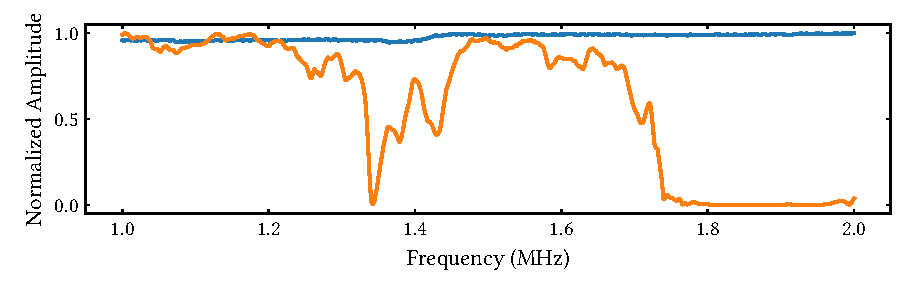
\includegraphics{figures/eom_amp_time_155.pdf}
}
\caption{Shown is the amplitude of a laser whose polarization was rotated by a pockels cell and then filtered using a polarizing beam splitter. The frequency is the repetition rate of the voltage placed into the \ac{eom}. The two materials are \ac{rtp} (orange) \ac{bbo} (blue). The curves are normalized to their maximum value.}
	%The amplitude of the pockels cell depends on the repitition rate of the signal. The signal in this case was applying $0$, $V_\pi$, $0$ and $-V_\pi$ repeatedly.}
\end{figure}

In order to measure the extinction ratio, the repetition rate is set to $\SI{100}{\kilo \hertz}$, where the amplitude is consistent. Measuring first the dark current of the photodiode and then taking the signal on the output of the beam splitter results in the extinction ratio found in Figure \ref{fig:eom_extc}.

\todo{think about the goodness of the fit}
\begin{figure}[t]
\label{fig:eom_extc}
\centering{
	\setlength{\figureheight}{2in}
	\setlength{\figurewidth}{\textwidth/2-2.5em}
	%% This file was created by tikzplotlib v0.9.4.
\begin{tikzpicture}

\definecolor{color0}{rgb}{0.12156862745098,0.466666666666667,0.705882352941177}
\definecolor{color1}{rgb}{1,0.498039215686275,0.0549019607843137}

\begin{groupplot}[group style={group size=2 by 1, horizontal sep=5em}]
\nextgroupplot[
height=\figureheight,
minor xtick={},
minor ytick={},
scaled y ticks=false,
tick align=inside,
tick pos=both,
width=\figurewidth,
x grid style={white!69.0196078431373!black},
xlabel={Time (ms)},
xmin=-5.00806, xmax=5.88194,
xtick style={color=black},
xtick={-6,-4,-2,0,2,4,6},
y grid style={white!69.0196078431373!black},
y tick label style={/pgf/number format/fixed},
ylabel style={align=center},
ylabel={Amplitude (a. u.)},
ymin=-0.00684806308564516, ymax=0.0267013484143548,
ytick style={color=black},
ytick={-0.01,-0.005,0,0.005,0.01,0.015,0.02,0.025,0.03}
]
\addplot [line width=1.5pt, color0]
table {%
-4.51306 0.0191854151643548
-4.49306 0.0197300451643548
-4.47306 0.0186407751643548
-4.45306 0.0189130951643548
-4.43306 0.0189130951643548
-4.41306 0.0191854151643548
-4.39306 0.0191854151643548
-4.37306 0.0186407751643548
-4.35306 0.0194577251643548
-4.33306 0.0183684651643548
-4.31306 0.0191854151643548
-4.29306 0.0189130951643548
-4.27306 0.0194577251643548
-4.25306 0.0189130951643548
-4.23306 0.0191854151643548
-4.21306 0.0194577251643548
-4.19306 0.0194577251643548
-4.17306 0.0194577251643548
-4.15306 0.0186407751643548
-4.13306 0.0186407751643548
-4.11306 0.0194577251643548
-4.09306 0.0189130951643548
-4.07306 0.0189130951643548
-4.05306 0.0189130951643548
-4.03306 0.0183684651643548
-4.01306 0.0189130951643548
-3.99306 0.0189130951643548
-3.97306 0.0183684651643548
-3.95306 0.0183684651643548
-3.93306 0.0186407751643548
-3.91306 0.0191854151643548
-3.89306 0.0191854151643548
-3.87306 0.0186407751643548
-3.85306 0.0194577251643548
-3.83306 0.0191854151643548
-3.81306 0.0186407751643548
-3.79306 0.0186407751643548
-3.77306 0.0191854151643548
-3.75306 0.0186407751643548
-3.73306 0.0191854151643548
-3.71306 0.0197300451643548
-3.69306 0.0189130951643548
-3.67306 0.0191854151643548
-3.65306 0.0194577251643548
-3.63306 0.0186407751643548
-3.61306 0.0186407751643548
-3.59306 0.0183684651643548
-3.57306 0.0197300451643548
-3.55306 0.0186407751643548
-3.53306 0.0191854151643548
-3.51306 0.0191854151643548
-3.49306 0.0186407751643548
-3.47306 0.0205469951643548
-3.45306 0.0167345651643548
-3.43306 0.0191854151643548
-3.41306 0.0200023651643548
-3.39306 0.0202746751643548
-3.37306 0.0183684651643548
-3.35306 0.0178238251643548
-3.33306 0.0208193151643548
-3.31306 0.0172791951643548
-3.29306 0.0183684651643548
-3.27306 0.0183684651643548
-3.25306 0.0205469951643548
-3.23306 0.0197300451643548
-3.21306 0.0183684651643548
-3.19306 0.0178238251643548
-3.17306 0.0178238251643548
-3.15306 0.0200023651643548
-3.13306 0.0191854151643548
-3.11306 0.0202746751643548
-3.09306 0.0178238251643548
-3.07306 0.0189130951643548
-3.05306 0.0191854151643548
-3.03306 0.0189130951643548
-3.01306 0.0200023651643548
-2.99306 0.0183684651643548
-2.97306 0.0186407751643548
-2.95306 0.0189130951643548
-2.93306 0.0200023651643548
-2.91306 0.0183684651643548
-2.89306 0.0194577251643548
-2.87306 0.0191854151643548
-2.85306 0.0202746751643548
-2.83306 0.0183684651643548
-2.81306 0.0191854151643548
-2.79306 0.0189130951643548
-2.77306 0.0186407751643548
-2.75306 0.0197300451643548
-2.73306 0.0186407751643548
-2.71306 0.0186407751643548
-2.69306 0.0183684651643548
-2.67306 0.0183684651643548
-2.65306 0.0194577251643548
-2.63306 0.0189130951643548
-2.61306 0.0200023651643548
-2.59306 0.0183684651643548
-2.57306 0.0194577251643548
-2.55306 0.0189130951643548
-2.53306 0.0189130951643548
-2.51306 0.0183684651643548
-2.49306 0.0205469951643548
-2.47306 0.0178238251643548
-2.45306 0.00475262816435484
-2.43306 -0.00532308983564516
-2.41306 0.00148482716435484
-2.39306 0.00121251116435484
-2.37306 -0.000421389335645161
-2.35306 0.000940194164354839
-2.33306 0.000940194164354839
-2.31306 0.00175714416435484
-2.29306 0.000667877164354839
-2.27306 0.000123244064354839
-2.25306 0.000940194164354839
-2.23306 0.000667877164354839
-2.21306 0.00121251116435484
-2.19306 0.000395561164354839
-2.17306 0.000395561164354839
-2.15306 0.00175714416435484
-2.13306 0.000940194164354839
-2.11306 -0.000421389335645161
-2.09306 0.000395561164354839
-2.07306 0.000667877164354839
-2.05306 0.00148482716435484
-2.03306 -0.000149072635645161
-2.01306 0.00202946116435484
-1.99306 0.000940194164354839
-1.97306 0.000395561164354839
-1.95306 0.000395561164354839
-1.93306 0.000123244064354839
-1.91306 0.000123244064354839
-1.89306 0.000395561164354839
-1.87306 0.000940194164354839
-1.85306 0.00121251116435484
-1.83306 0.000667877164354839
-1.81306 0.000940194164354839
-1.79306 0.000395561164354839
-1.77306 0.00121251116435484
-1.75306 0.000123244064354839
-1.73306 0.00121251116435484
-1.71306 0.000667877164354839
-1.69306 -0.000421389335645161
-1.67306 0.000395561164354839
-1.65306 0.000667877164354839
-1.63306 0.000395561164354839
-1.61306 -0.000421389335645161
-1.59306 0.000940194164354839
-1.57306 0.000940194164354839
-1.55306 0.000123244064354839
-1.53306 0.000940194164354839
-1.51306 0.000395561164354839
-1.49306 0.000940194164354839
-1.47306 0.000123244064354839
-1.45306 0.000123244064354839
-1.43306 0.000123244064354839
-1.41306 -0.000149072635645161
-1.39306 0.000667877164354839
-1.37306 0.000940194164354839
-1.35306 -0.000149072635645161
-1.33306 0.000395561164354839
-1.31306 0.00121251116435484
-1.29306 -0.000149072635645161
-1.27306 0.000667877164354839
-1.25306 0.000395561164354839
-1.23306 0.000123244064354839
-1.21306 0.000940194164354839
-1.19306 0.000395561164354839
-1.17306 0.000940194164354839
-1.15306 -0.000149072635645161
-1.13306 0.000940194164354839
-1.11306 0.000940194164354839
-1.09306 0.000940194164354839
-1.07306 0.000123244064354839
-1.05306 0.000395561164354839
-1.03306 0.000940194164354839
-1.01306 -0.000149072635645161
-0.993064 0.000667877164354839
-0.973064 0.000940194164354839
-0.953064 0.000395561164354839
-0.933064 -0.000149072635645161
-0.913064 0.000940194164354839
-0.893064 -0.000421389335645161
-0.873064 0.000940194164354839
-0.853064 0.000940194164354839
-0.833064 0.000395561164354839
-0.813064 0.000395561164354839
-0.793064 0.000667877164354839
-0.773064 0.000940194164354839
-0.753064 -0.000421389335645161
-0.733064 0.000667877164354839
-0.713064 0.000940194164354839
-0.693064 -0.000149072635645161
-0.673064 0.000667877164354839
-0.653064 0.000395561164354839
-0.633064 -0.000149072635645161
-0.613064 -0.000149072635645161
-0.593064 0.000667877164354839
-0.573064 -0.000421389335645161
-0.553064 0.000123244064354839
-0.533064 0.000395561164354839
-0.513064 -0.000149072635645161
-0.493064 0.000123244064354839
-0.473064 0.000940194164354839
-0.453064 0.000395561164354839
-0.433064 -0.000149072635645161
-0.413064 0.000940194164354839
-0.393064 0.000667877164354839
-0.373064 0.000123244064354839
-0.353064 0.000667877164354839
-0.333064 0.00121251116435484
-0.313064 0.000123244064354839
-0.293064 -0.000149072635645161
-0.273064 0.000667877164354839
-0.253064 0.000940194164354839
-0.233064 0.000395561164354839
-0.213064 -0.000149072635645161
-0.193064 -0.000421389335645161
-0.173064 0.000940194164354839
-0.153064 0.000395561164354839
-0.133064 0.000395561164354839
-0.113064 0.000123244064354839
-0.0930644 0.000395561164354839
-0.0730644 0.000395561164354839
-0.0530644 0.000123244064354839
-0.0330644 -0.000693706035645161
-0.0130644 0.000395561164354839
0.00693559 0.000940194164354839
0.0269356 0.000667877164354839
0.0469356 0.000395561164354839
0.0669356 -0.00123833933564516
0.0869356 0.000940194164354839
0.106936 -0.000149072635645161
0.126936 0.000395561164354839
0.146936 -0.000149072635645161
0.166936 0.000395561164354839
0.186936 0.000395561164354839
0.206936 0.000395561164354839
0.226936 0.000940194164354839
0.246936 0.000940194164354839
0.266936 -0.000149072635645161
0.286936 0.000123244064354839
0.306936 0.000395561164354839
0.326936 0.000940194164354839
0.346936 0.000667877164354839
0.366936 0.000940194164354839
0.386936 0.000123244064354839
0.406936 -0.000693706035645161
0.426936 0.000940194164354839
0.446936 0.000395561164354839
0.466936 0.000940194164354839
0.486936 0.000123244064354839
0.506936 0.000667877164354839
0.526936 0.000940194164354839
0.546936 -0.000149072635645161
0.566936 0.000395561164354839
0.586936 0.000940194164354839
0.606936 0.000395561164354839
0.626936 0.000123244064354839
0.646936 0.000395561164354839
0.666936 0.000395561164354839
0.686936 0.000395561164354839
0.706936 -0.000149072635645161
0.726936 0.000667877164354839
0.746936 -0.000149072635645161
0.766936 0.000123244064354839
0.786936 0.000395561164354839
0.806936 0.000123244064354839
0.826936 0.000667877164354839
0.846936 -0.000421389335645161
0.866936 0.000667877164354839
0.886936 0.000123244064354839
0.906936 -0.000149072635645161
0.926936 0.000940194164354839
0.946936 0.000395561164354839
0.966936 0.000395561164354839
0.986936 0.000123244064354839
1.00694 0.000940194164354839
1.02694 0.000395561164354839
1.04694 0.000123244064354839
1.06694 0.000395561164354839
1.08694 0.000395561164354839
1.10694 0.000395561164354839
1.12694 -0.000149072635645161
1.14694 0.000667877164354839
1.16694 0.000940194164354839
1.18694 -0.000149072635645161
1.20694 0.000395561164354839
1.22694 -0.000149072635645161
1.24694 0.000123244064354839
1.26694 0.000395561164354839
1.28694 0.000395561164354839
1.30694 0.000395561164354839
1.32694 0.000395561164354839
1.34694 0.000123244064354839
1.36694 0.000123244064354839
1.38694 0.00121251116435484
1.40694 -0.000693706035645161
1.42694 0.000667877164354839
1.44694 -0.000421389335645161
1.46694 0.000123244064354839
1.48694 -0.000421389335645161
1.50694 -0.000693706035645161
1.52694 0.000940194164354839
1.54694 -0.000149072635645161
1.56694 0.000667877164354839
1.58694 0.000123244064354839
1.60694 0.000123244064354839
1.62694 -0.000421389335645161
1.64694 0.000395561164354839
1.66694 0.000123244064354839
1.68694 -0.000149072635645161
1.70694 0.000940194164354839
1.72694 -0.000149072635645161
1.74694 0.000940194164354839
1.76694 0.000395561164354839
1.78694 -0.00123833933564516
1.80694 -0.000149072635645161
1.82694 0.000940194164354839
1.84694 0.000395561164354839
1.86694 0.00202946116435484
1.88694 0.000667877164354839
1.90694 0.000123244064354839
1.92694 -0.000966022735645161
1.94694 -0.000421389335645161
1.96694 0.00121251116435484
1.98694 -0.000149072635645161
2.00694 0.000667877164354839
2.02694 0.000395561164354839
2.04694 -0.000421389335645161
2.06694 0.000667877164354839
2.08694 0.000940194164354839
2.10694 0.000940194164354839
2.12694 0.000395561164354839
2.14694 -0.000149072635645161
2.16694 -0.000421389335645161
2.18694 0.000940194164354839
2.20694 0.000940194164354839
2.22694 -0.000421389335645161
2.24694 0.000123244064354839
2.26694 0.000940194164354839
2.28694 0.000123244064354839
2.30694 0.000395561164354839
2.32694 0.000395561164354839
2.34694 0.000123244064354839
2.36694 0.000123244064354839
2.38694 -0.000421389335645161
2.40694 0.000395561164354839
2.42694 0.000395561164354839
2.44694 0.000395561164354839
2.46694 0.000395561164354839
2.48694 -0.000149072635645161
2.50694 0.000123244064354839
2.52694 0.000395561164354839
2.54694 0.00910969416435484
2.56694 0.0251763751643548
2.58694 0.0186407751643548
2.60694 0.0145560251643548
2.62694 0.0189130951643548
2.64694 0.0183684651643548
2.66694 0.0178238251643548
2.68694 0.0178238251643548
2.70694 0.0178238251643548
2.72694 0.0183684651643548
2.74694 0.0178238251643548
2.76694 0.0178238251643548
2.78694 0.0183684651643548
2.80694 0.0186407751643548
2.82694 0.0186407751643548
2.84694 0.0183684651643548
2.86694 0.0178238251643548
2.88694 0.0186407751643548
2.90694 0.0183684651643548
2.92694 0.0178238251643548
2.94694 0.0186407751643548
2.96694 0.0183684651643548
2.98694 0.0186407751643548
3.00694 0.0189130951643548
3.02694 0.0186407751643548
3.04694 0.0175515151643548
3.06694 0.0186407751643548
3.08694 0.0186407751643548
3.10694 0.0180961451643548
3.12694 0.0183684651643548
3.14694 0.0194577251643548
3.16694 0.0183684651643548
3.18694 0.0191854151643548
3.20694 0.0189130951643548
3.22694 0.0186407751643548
3.24694 0.0189130951643548
3.26694 0.0186407751643548
3.28694 0.0191854151643548
3.30694 0.0180961451643548
3.32694 0.0189130951643548
3.34694 0.0189130951643548
3.36694 0.0189130951643548
3.38694 0.0200023651643548
3.40694 0.0183684651643548
3.42694 0.0186407751643548
3.44694 0.0186407751643548
3.46694 0.0189130951643548
3.48694 0.0186407751643548
3.50694 0.0191854151643548
3.52694 0.0186407751643548
3.54694 0.0194577251643548
3.56694 0.0194577251643548
3.58694 0.0191854151643548
3.60694 0.0191854151643548
3.62694 0.0189130951643548
3.64694 0.0197300451643548
3.66694 0.0183684651643548
3.68694 0.0191854151643548
3.70694 0.0191854151643548
3.72694 0.0186407751643548
3.74694 0.0191854151643548
3.76694 0.0191854151643548
3.78694 0.0186407751643548
3.80694 0.0194577251643548
3.82694 0.0191854151643548
3.84694 0.0186407751643548
3.86694 0.0183684651643548
3.88694 0.0194577251643548
3.90694 0.0197300451643548
3.92694 0.0197300451643548
3.94694 0.0183684651643548
3.96694 0.0183684651643548
3.98694 0.0202746751643548
4.00694 0.0186407751643548
4.02694 0.0189130951643548
4.04694 0.0189130951643548
4.06694 0.0200023651643548
4.08694 0.0178238251643548
4.10694 0.0194577251643548
4.12694 0.0175515151643548
4.14694 0.0197300451643548
4.16694 0.0191854151643548
4.18694 0.0194577251643548
4.20694 0.0191854151643548
4.22694 0.0197300451643548
4.24694 0.0189130951643548
4.26694 0.0194577251643548
4.28694 0.0191854151643548
4.30694 0.0189130951643548
4.32694 0.0189130951643548
4.34694 0.0186407751643548
4.36694 0.0191854151643548
4.38694 0.0183684651643548
4.40694 0.0189130951643548
4.42694 0.0197300451643548
4.44694 0.0191854151643548
4.46694 0.0200023651643548
4.48694 0.0189130951643548
4.50694 0.0194577251643548
4.52694 0.0183684651643548
4.54694 0.0191854151643548
4.56694 0.0197300451643548
4.58694 0.0183684651643548
4.60694 0.0183684651643548
4.62694 0.0200023651643548
4.64694 0.0183684651643548
4.66694 0.0183684651643548
4.68694 0.0186407751643548
4.70694 0.0189130951643548
4.72694 0.0186407751643548
4.74694 0.0194577251643548
4.76694 0.0189130951643548
4.78694 0.0194577251643548
4.80694 0.0183684651643548
4.82694 0.0194577251643548
4.84694 0.0191854151643548
4.86694 0.0186407751643548
4.88694 0.0175515151643548
4.90694 0.0189130951643548
4.92694 0.0191854151643548
4.94694 0.0191854151643548
4.96694 0.0183684651643548
4.98694 0.0194577251643548
5.00694 0.0191854151643548
5.02694 0.0191854151643548
5.04694 0.0191854151643548
5.06694 0.0189130951643548
5.08694 0.0194577251643548
5.10694 0.0191854151643548
5.12694 0.0191854151643548
5.14694 0.0186407751643548
5.16694 0.0197300451643548
5.18694 0.0186407751643548
5.20694 0.0186407751643548
5.22694 0.0197300451643548
5.24694 0.0189130951643548
5.26694 0.0194577251643548
5.28694 0.0183684651643548
5.30694 0.0194577251643548
5.32694 0.0194577251643548
5.34694 0.0197300451643548
5.36694 0.0186407751643548
5.38694 0.0197300451643548
};
\addplot [line width=1.5pt, color1, dashed]
table {%
-4.51306 0.0192932717552554
-4.49306 0.0193105152472244
-4.47306 0.0193194754466001
-4.45306 0.0193198861860666
-4.43306 0.019311702759259
-4.41306 0.0192951029399212
-4.39306 0.0192704826600563
-4.37306 0.0192384464450048
-4.35306 0.0191997928217822
-4.33306 0.019155495030766
-4.31306 0.0191066774775032
-4.29306 0.0190545884586945
-4.27306 0.0190005697822049
-4.25306 0.01894602397337
-4.23306 0.0188923798173238
-4.21306 0.018841057028294
-4.19306 0.0187934308608322
-4.17306 0.0187507974842101
-4.15306 0.0187143409294841
-4.13306 0.0186851023891957
-4.11306 0.0186639526028562
-4.09306 0.0186515679981872
-4.07306 0.0186484111797911
-4.05306 0.0186547162650967
-4.03306 0.0186704794639303
-4.01306 0.0186954551850257
-3.99306 0.0187291578325461
-3.97306 0.0187708693307452
-3.95306 0.0188196522878604
-3.93306 0.0188743685838846
-3.91306 0.018933703043684
-3.89306 0.0189961917396485
-3.87306 0.0190602543592202
-3.85306 0.0191242299745972
-3.83306 0.0191864154668433
-3.81306 0.0192451057864565
-3.79306 0.0192986351787853
-3.77306 0.0193454184668364
-3.75306 0.0193839914669325
-3.73306 0.0194130496149158
-3.71306 0.0194314839023381
-3.69306 0.019438413263095
-3.67306 0.0194332126106451
-3.65306 0.0194155358032932
-3.63306 0.0193853329086328
-3.61306 0.0193428612464274
-3.59306 0.0192886898099227
-3.57306 0.0192236967965274
-3.55306 0.0191490601174309
-3.53306 0.0190662408993417
-3.51306 0.0189769601372754
-3.49306 0.0188831688022828
-3.47306 0.0187870118492568
-3.45306 0.0186907867046052
-3.43306 0.0185968969388332
-3.41306 0.0185078019423205
-3.39306 0.0184259635213819
-3.37306 0.0183537904139117
-3.35306 0.0182935817876725
-3.33306 0.0182474708280952
-3.31306 0.0182173695451749
-3.29306 0.01820491592994
-3.27306 0.0182114245697467
-3.25306 0.0182378417883999
-3.23306 0.0182847063124079
-3.21306 0.0183521163794801
-3.19306 0.0184397041010908
-3.17306 0.0185466177692926
-3.15306 0.0186715126611159
-3.13306 0.0188125507442539
-3.11306 0.0189674095280195
-3.09306 0.0191333001366991
-3.07306 0.0193069945115044
-3.05306 0.0194848614755435
-3.03306 0.0196629112268434
-3.01306 0.0198368476606854
-2.99306 0.0200021277675251
-2.97306 0.0201540272095697
-2.95306 0.0202877110505091
-2.93306 0.0203983085014979
-2.91306 0.0204809904545475
-2.89306 0.0205310485039156
-2.87306 0.0205439741084153
-2.85306 0.0205155365239227
-2.83306 0.0204418581364072
-2.81306 0.0203194858517665
-2.79306 0.0201454572493635
-2.77306 0.0199173602807247
-2.75306 0.0196333853922115
-2.73306 0.0192923690690123
-2.71306 0.0188938279355346
-2.69306 0.0184379827018248
-2.67306 0.0179257714143185
-2.65306 0.0173588516490463
-2.63306 0.0167395914731999
-2.61306 0.0160710491933257
-2.59306 0.015356942101907
-2.57306 0.0146016046252101
-2.55306 0.0138099364605241
-2.53306 0.0129873414669471
-2.51306 0.0121396582374213
-2.49306 0.0112730834277867
-2.47306 0.010394089048474
-2.45306 0.00950933503366322
-2.43306 0.00862557848926327
-2.41306 0.0077495810832746
-2.39306 0.00688801607878963
-2.37306 0.006047376520338
-2.35306 0.00523388606823347
-2.33306 0.00445341393326998
-2.31306 0.00371139529625196
-2.29306 0.00301275850461105
-2.27306 0.00236186022338972
-2.25306 0.00176242958220268
-2.23306 0.00121752220585071
-2.21306 0.000729484846814451
-2.19306 0.00029993115594793
-2.17306 -7.02710634075936e-05
-2.15306 -0.000381000969516354
-2.13306 -0.000632874215226602
-2.11306 -0.000827221148189602
-2.09306 -0.000966054119418242
-2.07306 -0.00105202452563901
-2.05306 -0.0010883703835544
-2.03306 -0.0010788553920246
-2.01306 -0.00102770057849116
-1.99306 -0.00093950974622543
-1.97306 -0.000819190037086826
-1.95306 -0.000671868998728946
-1.93306 -0.000502809594346653
-1.91306 -0.000317324616329717
-1.89306 -0.000120691962273635
-1.87306 8.19277971274499e-05
-1.85306 0.000285570183061291
-1.83306 0.000485540609721431
-1.81306 0.000677482026029462
-1.79306 0.000857435324290915
-1.77306 0.00102189158234564
-1.75306 0.00116783536166645
-1.73306 0.00129277845246367
-1.71306 0.00139478363499051
-1.69306 0.00147247821057697
-1.67306 0.00152505724301159
-1.65306 0.00155227663727145
-1.63306 0.00155443636483512
-1.61306 0.00153235431955976
-1.59306 0.00148733145218174
-1.57306 0.00142110898194713
-1.55306 0.00133581861800422
-1.53306 0.00123392683862872
-1.51306 0.00111817437110071
-1.49306 0.000991512087513277
-1.47306 0.000857034580794072
-1.45306 0.000717912710046141
-1.43306 0.000577326404702719
-1.41306 0.000438398993149205
-1.39306 0.000304134274057588
-1.37306 0.000177357478808758
-1.35306 6.06611825714788e-05
-1.33306 -4.36428882244315e-05
-1.31306 -0.000133565330879201
-1.29306 -0.000207473143531886
-1.27306 -0.000264115876217804
-1.25306 -0.000302643488249821
-1.23306 -0.000322615710056817
-1.21306 -0.000324002875353693
-1.19306 -0.000307178355995686
-1.17306 -0.00027290289388875
-1.15306 -0.00022230127879864
-1.13306 -0.000156831964904782
-1.11306 -7.82503497844065e-05
-1.09306 1.1433445233619e-05
-1.07306 0.000110001356839348
-1.05306 0.00021507770899497
-1.03306 0.000324182017676708
-1.01306 0.000434783163480877
-0.993064 0.000544332166065919
-0.973064 0.000650403258946407
-0.953064 0.000750613263206291
-0.933064 0.000842758668899668
-0.913064 0.000924838233475255
-0.893064 0.000995092880769875
-0.873064 0.00105204003925455
-0.853064 0.00109450177991163
-0.833064 0.0011216262466384
-0.813064 0.00113290201352862
-0.793064 0.00112816515089649
-0.773064 0.00110759893249333
-0.753064 0.0010717262670005
-0.733064 0.00102139508455416
-0.713064 0.00095775705083838
-0.693064 0.000882240114375793
-0.673064 0.000796515514444041
-0.653064 0.000702459985183613
-0.633064 0.000602113983858408
-0.613064 0.00049763684612928
-0.593064 0.000391259827205869
-0.573064 0.000285238023843766
-0.553064 0.000181802187743801
-0.533064 8.31114357950757e-05
-0.513064 -8.79216299380821e-06
-0.493064 -9.20261894787021e-05
-0.473064 -0.000164906795151765
-0.453064 -0.000225983153264338
-0.433064 -0.000274066749229267
-0.413064 -0.00030825493021819
-0.393064 -0.000327948256158873
-0.373064 -0.000332861325392493
-0.353064 -0.000323026885365774
-0.333064 -0.000298793179092859
-0.313064 -0.000260814618853548
-0.293064 -0.000210036016830418
-0.273064 -0.000147670735317114
-0.253064 -7.51732440617582e-05
-0.233064 5.79331327977411e-06
-0.213064 9.3393840018061e-05
-0.193064 0.000185661504340557
-0.173064 0.000280540593825793
-0.153064 0.000375931093965805
-0.133064 0.000469734044934831
-0.113064 0.000559896717307199
-0.0930644 0.000644455031045084
-0.0730644 0.000721582192954207
-0.0530644 0.000789617531963582
-0.0330644 0.000847108697404784
-0.0130644 0.000892840682615096
0.00693559 0.000925861446270299
0.0269356 0.000945501935811443
0.0469356 0.000951389820526611
0.0669356 0.000943457109511566
0.0869356 0.000921941038938914
0.106936 0.000887377673018551
0.126936 0.000840592912852212
0.146936 0.000782680127989067
0.166936 0.000714978692770273
0.186936 0.000639044159361673
0.206936 0.000556614330753605
0.226936 0.000469571386553066
0.246936 0.000379900861001505
0.266936 0.000289648339698228
0.286936 0.000200874790667988
0.306936 0.000115611475646968
0.326936 3.58153981275446e-05
0.346936 -3.66737644551616e-05
0.366936 -0.000100174325838736
0.386936 -0.000153199982740248
0.406936 -0.000194493128864499
0.426936 -0.00022305336960652
0.446936 -0.000238160614125151
0.466936 -0.000239392232877483
0.486936 -0.000226633891098855
0.506936 -0.000200083799614444
0.526936 -0.000160250261120928
0.546936 -0.000107942529897974
0.566936 -4.42551429472651e-05
0.586936 2.94539820554253e-05
0.606936 0.000111591254693635
0.626936 0.000200360374604917
0.646936 0.000293799885147645
0.666936 0.000389824554100844
0.686936 0.000486269732922907
0.706936 0.000580937778476776
0.726936 0.000671645571991522
0.746936 0.000756272140472166
0.766936 0.000832805376496395
0.786936 0.000899386863651142
0.806936 0.000954353846650353
0.826936 0.000996277436911543
0.846936 0.0010239962151232
0.866936 0.00103664448078979
0.886936 0.00103367450321573
0.906936 0.00101487224687229
0.926936 0.000980366174279549
0.946936 0.000930628868877073
0.966936 0.000866471366102994
0.986936 0.000789030230158417
1.00694 0.000699728633223696
1.02694 0.000600323519694849
1.04694 0.000492764964810623
1.06694 0.000379226973059697
1.08694 0.000262047213026617
1.10694 0.000143679405314786
1.12694 2.66425720585016e-05
1.14694 -8.65318429362997e-05
1.16694 -0.000193353918921427
1.18694 -0.000291429168641284
1.20694 -0.000378511302306289
1.22694 -0.000452552742039068
1.24694 -0.000511751814940502
1.26694 -0.00055459560582149
1.28694 -0.000579897524374984
1.30694 -0.000586828734850824
1.32694 -0.000574942707479468
1.34694 -0.00054419227794497
1.36694 -0.000494938741781281
1.38694 -0.000427952662028703
1.40694 -0.000344406227976797
1.42694 -0.000245857167296321
1.44694 -0.000134224380169856
1.46694 -1.17556289505397e-05
1.48694 0.000119012222798752
1.50694 0.000255299775455244
1.52694 0.000394137674428533
1.54694 0.0005324242907267
1.56694 0.000666987472490874
1.58694 0.000794649245437464
1.60694 0.000912292267030574
1.62694 0.00101692678810997
1.64694 0.00110575684778871
1.66694 0.00117624442344392
1.68694 0.00122617027783398
1.70694 0.00125369028960781
1.72694 0.0012573861210901
1.74694 0.0012363091671447
1.76694 0.00119001683962115
1.78694 0.00111860037145857
1.80694 0.00102270347066799
1.82694 0.000903531314525221
1.84694 0.0007628495454874
1.86694 0.00060297310947947
1.88694 0.00042674496099503
1.90694 0.000237504844529684
1.92694 3.9048544778637e-05
1.94694 -0.000164421824625305
1.96694 -0.00036835575560667
1.98694 -0.000567919608765333
2.00694 -0.000758068169154951
2.02694 -0.000933621335134131
2.04694 -0.00108934467718246
2.06694 -0.00122003252217319
2.08694 -0.00132059216092498
2.10694 -0.00138612774409286
2.12694 -0.00141202242432397
2.14694 -0.00139401732134274
2.16694 -0.00132828593101322
2.18694 -0.0012115026687464
2.20694 -0.00104090433071137
2.22694 -0.000814343371559289
2.24694 -0.000530332032757768
2.26694 -0.000188076508762135
2.28694 0.000212499493609443
2.30694 0.000670742267087542
2.32694 0.00118526696273029
2.34694 0.00175396787687313
2.36694 0.00237404005141034
2.38694 0.0030420118781008
2.40694 0.00375378820830509
2.42694 0.00450470328887641
2.44694 0.00528958267610332
2.46694 0.00610281312567575
2.48694 0.00693841932039011
2.50694 0.00779014618115893
2.52694 0.00865154541292341
2.54694 0.0095160648669403
2.56694 0.0103771392558563
2.58694 0.0112282807387526
2.60694 0.0120631679002309
2.62694 0.0128757316804279
2.64694 0.0136602368709233
2.66694 0.0144113578737224
2.68694 0.0151242475252818
2.70694 0.0157945979129338
2.72694 0.016418692254701
2.74694 0.0169934470727222
2.76694 0.0175164440623598
2.78694 0.0179859512403944
2.80694 0.0184009331431735
2.82694 0.0187610500357721
2.84694 0.0190666462826634
2.86694 0.0193187282156758
2.88694 0.019518932012781
2.90694 0.0196694822683607
2.92694 0.0197731420890497
2.94694 0.0198331556863873
2.96694 0.0198531845559324
2.98694 0.0198372384302093
3.00694 0.0197896022682408
3.02694 0.0197147605962883
3.04694 0.0196173205420327
3.06694 0.0195019349074871
3.08694 0.0193732266046217
3.10694 0.0192357157326171
3.12694 0.0190937505079159
3.14694 0.0189514431692875
3.16694 0.0188126118718338
3.18694 0.0186807294584415
3.20694 0.0185588798571613
3.22694 0.0184497227011247
3.24694 0.018355466606868
3.26694 0.0182778513804287
3.28694 0.0182181392515055
3.30694 0.0181771150675321
3.32694 0.0181550952148867
3.34694 0.0181519448766974
3.36694 0.0181671030887233
3.38694 0.0181996149192816
3.40694 0.0182481699785712
3.42694 0.0183111463591488
3.44694 0.0183866590244881
3.46694 0.0184726115979139
3.48694 0.018566750460719
3.50694 0.0186667200465195
3.52694 0.0187701182190262
3.54694 0.0188745506421214
3.56694 0.0189776830937284
3.58694 0.0190772907373531
3.60694 0.0191713034458753
3.62694 0.0192578463693672
3.64694 0.0193352750502829
3.66694 0.0194022045129163
3.68694 0.0194575318869708
3.70694 0.0195004522646594
3.72694 0.0195304676341139
3.74694 0.0195473888761023
3.76694 0.0195513309532622
3.78694 0.0195427015584121
3.80694 0.019522183618314
3.82694 0.0194907121690039
3.84694 0.0194494462261804
3.86694 0.0193997363671262
3.88694 0.0193430888175079
3.90694 0.0192811268957868
3.92694 0.0192155507088552
3.94694 0.019148096014272
3.96694 0.0190804931668649
3.98694 0.0190144270506628
4.00694 0.0189514988616597
4.02694 0.0188931905537349
4.04694 0.0188408326904211
4.06694 0.0187955763607517
4.08694 0.0187583697200132
4.10694 0.0187299396080372
4.12694 0.0187107785810417
4.14694 0.0187011375704917
4.16694 0.0187010242566024
4.18694 0.0187102071176377
4.20694 0.0187282249917155
4.22694 0.0187544018680332
4.24694 0.0187878665117661
4.26694 0.0188275764236952
4.28694 0.0188723455440238
4.30694 0.0189208750317023
4.32694 0.0189717863874891
4.34694 0.0190236561421874
4.36694 0.0190750513019251
4.38694 0.019124564730544
4.40694 0.0191708496553026
4.42694 0.0192126525059766
4.44694 0.0192488433384914
4.46694 0.0192784431515024
4.48694 0.0193006474765856
4.50694 0.0193148457083313
4.52694 0.0193206357377735
4.54694 0.0193178335591503
4.56694 0.0193064776336637
4.58694 0.0192868279122526
4.60694 0.0192593595398611
4.62694 0.0192247513836881
4.64694 0.0191838696448659
4.66694 0.0191377469244122
4.68694 0.0190875572177355
4.70694 0.0190345874052095
4.72694 0.018980205887335
4.74694 0.0189258290800235
4.76694 0.0188728865370601
4.78694 0.0188227855017056
4.80694 0.0187768757068369
4.82694 0.0187364152425854
4.84694 0.0187025382920191
4.86694 0.0186762254993478
4.88694 0.0186582776820867
4.90694 0.0186492935296277
4.92694 0.0186496518471235
4.94694 0.0186594988071749
4.96694 0.0186787405644965
4.98694 0.0187070414727268
5.00694 0.018743828020256
5.02694 0.0187882984759075
5.04694 0.0188394381081811
5.06694 0.0188960397162237
5.08694 0.0189567290894156
5.10694 0.0190199948980346
5.12694 0.0190842224123817
5.14694 0.0191477303543034
5.16694 0.0192088101053256
5.18694 0.0192657664314237
5.20694 0.0193169588373009
5.22694 0.0193608426341156
5.24694 0.0193960087946693
5.26694 0.0194212216795883
5.28694 0.0194354537470108
5.30694 0.0194379164063667
5.32694 0.0194280862432434
5.34694 0.0194057259259242
5.36694 0.0193708992034513
5.38694 0.0193239795181823
};

\nextgroupplot[
height=\figureheight,
minor xtick={},
minor ytick={},
scaled y ticks=false,
tick align=inside,
tick pos=both,
width=\figurewidth,
x grid style={white!69.0196078431373!black},
xlabel={Time (ms)},
xmin=-10.4293315, xmax=11.3507015,
xtick style={color=black},
xtick={-15,-10,-5,0,5,10,15},
y grid style={white!69.0196078431373!black},
y tick label style={/pgf/number format/fixed},
ylabel style={align=center},
ylabel={Amplitude (a. u.)},
ymin=-0.0147315379356452, ymax=0.0722397662643548,
ytick style={color=black},
ytick={-0.02,-0.01,0,0.01,0.02,0.03,0.04,0.05,0.06,0.07,0.08}
]
\addplot [line width=1.5pt, color0]
table {%
-9.43933 0.0529836551643548
-9.39933 0.0521334951643548
-9.35933 0.0529836551643548
-9.31933 0.0534087351643548
-9.27933 0.0529836551643548
-9.23933 0.0538338151643548
-9.19933 0.0542588951643548
-9.15933 0.0538338151643548
-9.11933 0.0538338151643548
-9.07933 0.0542588951643548
-9.03933 0.0542588951643548
-8.99933 0.0534087351643548
-8.95933 0.0534087351643548
-8.91933 0.0542588951643548
-8.87933 0.0538338151643548
-8.83933 0.0546839751643548
-8.79933 0.0538338151643548
-8.75933 0.0542588951643548
-8.71933 0.0542588951643548
-8.67933 0.0551090551643548
-8.63933 0.0538338151643548
-8.59933 0.0538338151643548
-8.55933 0.0538338151643548
-8.51933 0.0551090551643548
-8.47933 0.0538338151643548
-8.43933 0.0542588951643548
-8.39933 0.0542588951643548
-8.35933 0.0542588951643548
-8.31933 0.0542588951643548
-8.27933 0.0542588951643548
-8.23933 0.0529836551643548
-8.19933 0.0546839751643548
-8.15933 0.0538338151643548
-8.11933 0.0534087351643548
-8.07933 0.0538338151643548
-8.03933 0.0534087351643548
-7.99933 0.0542588951643548
-7.95933 0.0538338151643548
-7.91933 0.0542588951643548
-7.87933 0.0538338151643548
-7.83933 0.0538338151643548
-7.79933 0.0551090551643548
-7.75933 0.0546839751643548
-7.71933 0.0546839751643548
-7.67933 0.0542588951643548
-7.63933 0.0542588951643548
-7.59933 0.0551090551643548
-7.55933 0.0551090551643548
-7.51933 0.0559592151643548
-7.47933 0.0555341351643548
-7.43933 0.0551090551643548
-7.39933 0.0546839751643548
-7.35933 0.0551090551643548
-7.31933 0.0546839751643548
-7.27933 0.0546839751643548
-7.23933 0.0555341351643548
-7.19933 0.0546839751643548
-7.15933 0.0551090551643548
-7.11933 0.0559592151643548
-7.07933 0.0551090551643548
-7.03933 0.0546839751643548
-6.99933 0.0551090551643548
-6.95933 0.0551090551643548
-6.91933 0.0542588951643548
-6.87933 0.0542588951643548
-6.83933 0.0538338151643548
-6.79933 0.0542588951643548
-6.75933 0.0555341351643548
-6.71933 0.0546839751643548
-6.67933 0.0551090551643548
-6.63933 0.0551090551643548
-6.59933 0.0542588951643548
-6.55933 0.0542588951643548
-6.51933 0.0546839751643548
-6.47933 0.0546839751643548
-6.43933 0.0555341351643548
-6.39933 0.0551090551643548
-6.35933 0.0542588951643548
-6.31933 0.0546839751643548
-6.27933 0.0542588951643548
-6.23933 0.0546839751643548
-6.19933 0.0546839751643548
-6.15933 0.0551090551643548
-6.11933 0.0551090551643548
-6.07933 0.0551090551643548
-6.03933 0.0555341351643548
-5.99933 0.0542588951643548
-5.95933 0.0555341351643548
-5.91933 0.0538338151643548
-5.87933 0.0546839751643548
-5.83933 0.0525585751643548
-5.79933 0.0568093751643548
-5.75933 0.0546839751643548
-5.71933 0.0585096951643548
-5.67933 0.0572344551643548
-5.63933 0.0563842951643548
-5.59933 0.0551090551643548
-5.55933 0.0559592151643548
-5.51933 0.0538338151643548
-5.47933 0.0559592151643548
-5.43933 0.0546839751643548
-5.39933 0.0555341351643548
-5.35933 0.0538338151643548
-5.31933 0.0551090551643548
-5.27933 0.0542588951643548
-5.23933 0.0559592151643548
-5.19933 0.0551090551643548
-5.15933 0.0546839751643548
-5.11933 0.0555341351643548
-5.07933 0.0555341351643548
-5.03933 0.0529836551643548
-4.99933 0.0546839751643548
-4.95933 0.0542588951643548
-4.91933 0.0529836551643548
-4.87933 0.0538338151643548
-4.83933 -0.00992813783564516
-4.79933 0.00537473216435484
-4.75933 0.00452457216435484
-4.71933 0.00367441316435484
-4.67933 0.00324933316435484
-4.63933 0.00239917416435484
-4.59933 0.00282425316435484
-4.55933 0.00324933316435484
-4.51933 0.00282425316435484
-4.47933 0.00239917416435484
-4.43933 0.00324933316435484
-4.39933 0.00197409416435484
-4.35933 0.00239917416435484
-4.31933 0.00154901416435484
-4.27933 0.00197409416435484
-4.23933 0.00112393516435484
-4.19933 0.00154901416435484
-4.15933 0.00112393516435484
-4.11933 0.00197409416435484
-4.07933 0.00197409416435484
-4.03933 0.00239917416435484
-3.99933 0.00112393516435484
-3.95933 0.00154901416435484
-3.91933 0.00154901416435484
-3.87933 0.00154901416435484
-3.83933 0.00154901416435484
-3.79933 0.00154901416435484
-3.75933 0.00154901416435484
-3.71933 0.00154901416435484
-3.67933 0.000698855164354839
-3.63933 0.00112393516435484
-3.59933 0.00154901416435484
-3.55933 0.00197409416435484
-3.51933 0.00154901416435484
-3.47933 0.00154901416435484
-3.43933 0.00197409416435484
-3.39933 0.00112393516435484
-3.35933 0.00197409416435484
-3.31933 0.000698855164354839
-3.27933 0.00154901416435484
-3.23933 0.00197409416435484
-3.19933 0.00197409416435484
-3.15933 0.00197409416435484
-3.11933 0.00239917416435484
-3.07933 0.00112393516435484
-3.03933 0.000698855164354839
-2.99933 0.00112393516435484
-2.95933 0.00112393516435484
-2.91933 0.00112393516435484
-2.87933 0.00112393516435484
-2.83933 0.00112393516435484
-2.79933 0.00112393516435484
-2.75933 0.000698855164354839
-2.71933 0.000698855164354839
-2.67933 0.00112393516435484
-2.63933 0.000273775164354839
-2.59933 0.000698855164354839
-2.55933 0.00112393516435484
-2.51933 0.00112393516435484
-2.47933 0.00154901416435484
-2.43933 0.00197409416435484
-2.39933 0.00112393516435484
-2.35933 0.000698855164354839
-2.31933 0.00154901416435484
-2.27933 -0.000151304335645161
-2.23933 0.00112393516435484
-2.19933 0.000273775164354839
-2.15933 0.000698855164354839
-2.11933 0.000698855164354839
-2.07933 0.000698855164354839
-2.03933 0.00154901416435484
-1.99933 0.000698855164354839
-1.95933 0.00112393516435484
-1.91933 0.000273775164354839
-1.87933 0.00112393516435484
-1.83933 0.00112393516435484
-1.79933 0.00112393516435484
-1.75933 0.00112393516435484
-1.71933 0.000698855164354839
-1.67933 0.000273775164354839
-1.63933 0.00112393516435484
-1.59933 0.000273775164354839
-1.55933 0.000698855164354839
-1.51933 0.000273775164354839
-1.47933 0.000698855164354839
-1.43933 0.00154901416435484
-1.39933 0.000698855164354839
-1.35933 -0.000151304335645161
-1.31933 0.00154901416435484
-1.27933 0.000698855164354839
-1.23933 0.00112393516435484
-1.19933 0.00154901416435484
-1.15933 -0.000151304335645161
-1.11933 -0.000151304335645161
-1.07933 0.00239917416435484
-1.03933 0.000273775164354839
-0.999325 0.00197409416435484
-0.959325 0.000698855164354839
-0.919325 0.00112393516435484
-0.879325 0.000273775164354839
-0.839325 0.00154901416435484
-0.799325 -0.000576384035645161
-0.759325 0.000273775164354839
-0.719325 0.000698855164354839
-0.679325 0.00154901416435484
-0.639325 0.00112393516435484
-0.599325 0.00197409416435484
-0.559325 0.000273775164354839
-0.519325 0.000273775164354839
-0.479325 0.000698855164354839
-0.439325 0.00112393516435484
-0.399325 0.00112393516435484
-0.359325 0.000698855164354839
-0.319325 0.00112393516435484
-0.279325 0.000698855164354839
-0.239325 0.00112393516435484
-0.199325 0.000273775164354839
-0.159325 0.00154901416435484
-0.119325 0.000273775164354839
-0.0793255 0.00154901416435484
-0.0393255 0.00112393516435484
0.000674544 0.00112393516435484
0.0406745 0.000698855164354839
0.0806745 0.000273775164354839
0.120675 0.00112393516435484
0.160675 0.0682865251643548
0.200675 0.0504331851643548
0.240675 0.0504331851643548
0.280675 0.0512833351643548
0.320675 0.0517084151643548
0.360675 0.0517084151643548
0.400675 0.0517084151643548
0.440675 0.0517084151643548
0.480675 0.0521334951643548
0.520675 0.0508582551643548
0.560675 0.0525585751643548
0.600675 0.0534087351643548
0.640675 0.0521334951643548
0.680675 0.0529836551643548
0.720675 0.0521334951643548
0.760675 0.0534087351643548
0.800675 0.0534087351643548
0.840675 0.0538338151643548
0.880675 0.0551090551643548
0.920675 0.0546839751643548
0.960675 0.0538338151643548
1.00067 0.0534087351643548
1.04067 0.0546839751643548
1.08067 0.0542588951643548
1.12067 0.0546839751643548
1.16067 0.0555341351643548
1.20067 0.0534087351643548
1.24067 0.0546839751643548
1.28067 0.0551090551643548
1.32067 0.0551090551643548
1.36067 0.0546839751643548
1.40067 0.0542588951643548
1.44067 0.0542588951643548
1.48067 0.0538338151643548
1.52067 0.0542588951643548
1.56067 0.0538338151643548
1.60067 0.0546839751643548
1.64067 0.0542588951643548
1.68067 0.0534087351643548
1.72067 0.0529836551643548
1.76067 0.0538338151643548
1.80067 0.0538338151643548
1.84067 0.0538338151643548
1.88067 0.0525585751643548
1.92067 0.0538338151643548
1.96067 0.0546839751643548
2.00067 0.0542588951643548
2.04067 0.0538338151643548
2.08067 0.0551090551643548
2.12067 0.0546839751643548
2.16067 0.0546839751643548
2.20067 0.0542588951643548
2.24067 0.0542588951643548
2.28067 0.0551090551643548
2.32067 0.0546839751643548
2.36067 0.0538338151643548
2.40067 0.0551090551643548
2.44067 0.0563842951643548
2.48067 0.0546839751643548
2.52067 0.0551090551643548
2.56067 0.0546839751643548
2.60067 0.0546839751643548
2.64067 0.0546839751643548
2.68067 0.0542588951643548
2.72067 0.0546839751643548
2.76067 0.0551090551643548
2.80067 0.0551090551643548
2.84067 0.0555341351643548
2.88067 0.0555341351643548
2.92067 0.0546839751643548
2.96067 0.0551090551643548
3.00067 0.0555341351643548
3.04067 0.0546839751643548
3.08067 0.0542588951643548
3.12067 0.0551090551643548
3.16067 0.0542588951643548
3.20067 0.0542588951643548
3.24067 0.0542588951643548
3.28067 0.0546839751643548
3.32067 0.0538338151643548
3.36067 0.0546839751643548
3.40067 0.0551090551643548
3.44067 0.0538338151643548
3.48067 0.0555341351643548
3.52067 0.0542588951643548
3.56067 0.0542588951643548
3.60067 0.0546839751643548
3.64067 0.0542588951643548
3.68067 0.0551090551643548
3.72067 0.0563842951643548
3.76067 0.0551090551643548
3.80067 0.0551090551643548
3.84067 0.0542588951643548
3.88067 0.0546839751643548
3.92067 0.0546839751643548
3.96067 0.0551090551643548
4.00067 0.0546839751643548
4.04067 0.0551090551643548
4.08067 0.0559592151643548
4.12067 0.0555341351643548
4.16067 0.0555341351643548
4.20067 0.0546839751643548
4.24067 0.0555341351643548
4.28067 0.0551090551643548
4.32067 0.0546839751643548
4.36067 0.0555341351643548
4.40067 0.0546839751643548
4.44067 0.0563842951643548
4.48067 0.0551090551643548
4.52067 0.0555341351643548
4.56067 0.0551090551643548
4.60067 0.0551090551643548
4.64067 0.0551090551643548
4.68067 0.0538338151643548
4.72067 0.0542588951643548
4.76067 0.0551090551643548
4.80067 0.0542588951643548
4.84067 0.0546839751643548
4.88067 0.0538338151643548
4.92067 0.0538338151643548
4.96067 0.0542588951643548
5.00067 0.0555341351643548
5.04067 0.0538338151643548
5.08067 0.0551090551643548
5.12067 0.0525585751643548
5.16067 -0.0107782968356452
5.20067 0.00494965216435484
5.24067 0.00452457216435484
5.28067 0.00282425316435484
5.32067 0.00197409416435484
5.36067 0.00324933316435484
5.40067 0.00112393516435484
5.44067 0.00282425316435484
5.48067 0.00197409416435484
5.52067 0.00197409416435484
5.56067 0.00239917416435484
5.60067 0.00324933316435484
5.64067 0.00112393516435484
5.68067 0.00239917416435484
5.72067 0.00197409416435484
5.76067 0.00112393516435484
5.80067 0.00197409416435484
5.84067 0.00112393516435484
5.88067 0.00154901416435484
5.92067 0.00112393516435484
5.96067 0.00112393516435484
6.00067 0.00197409416435484
6.04067 0.00197409416435484
6.08067 0.00197409416435484
6.12067 0.00197409416435484
6.16067 0.000698855164354839
6.20067 0.00197409416435484
6.24067 0.00112393516435484
6.28067 0.00282425316435484
6.32067 0.00197409416435484
6.36067 0.00154901416435484
6.40067 0.00154901416435484
6.44067 0.000698855164354839
6.48067 0.00154901416435484
6.52067 0.000698855164354839
6.56067 0.00154901416435484
6.60067 0.00112393516435484
6.64067 0.00239917416435484
6.68067 0.00197409416435484
6.72067 0.00112393516435484
6.76067 0.00112393516435484
6.80067 0.000698855164354839
6.84067 0.000698855164354839
6.88067 0.000273775164354839
6.92067 0.00112393516435484
6.96067 0.000698855164354839
7.00067 -0.000151304335645161
7.04067 0.000273775164354839
7.08067 0.00154901416435484
7.12067 0.00154901416435484
7.16067 0.00112393516435484
7.20067 0.00112393516435484
7.24067 0.00112393516435484
7.28067 0.000698855164354839
7.32067 0.000698855164354839
7.36067 0.00112393516435484
7.40067 0.000698855164354839
7.44067 0.00154901416435484
7.48067 0.000698855164354839
7.52067 0.000273775164354839
7.56067 0.00112393516435484
7.60067 0.00112393516435484
7.64067 0.000273775164354839
7.68067 0.000273775164354839
7.72067 0.000273775164354839
7.76067 0.000698855164354839
7.80067 0.00112393516435484
7.84067 0.000698855164354839
7.88067 0.000698855164354839
7.92067 0.000698855164354839
7.96067 0.00112393516435484
8.00067 0.00197409416435484
8.04067 0.00197409416435484
8.08067 0.00112393516435484
8.12067 0.00112393516435484
8.16067 0.000273775164354839
8.20067 0.000273775164354839
8.24067 0.000273775164354839
8.28067 -0.000151304335645161
8.32067 0.00112393516435484
8.36067 0.000698855164354839
8.40067 0.000273775164354839
8.44067 0.000273775164354839
8.48067 0.000273775164354839
8.52067 0.000273775164354839
8.56067 0.000273775164354839
8.60067 0.00112393516435484
8.64067 0.00197409416435484
8.68067 0.00112393516435484
8.72067 0.00112393516435484
8.76067 0.000698855164354839
8.80067 0.000698855164354839
8.84067 0.00154901416435484
8.88067 0.00154901416435484
8.92067 0.000698855164354839
8.96067 0.00112393516435484
9.00067 0.000273775164354839
9.04067 0.00112393516435484
9.08067 0.000698855164354839
9.12067 0.000273775164354839
9.16067 -0.000576384035645161
9.20067 0.00112393516435484
9.24067 -0.000576384035645161
9.28067 0.00324933316435484
9.32067 -0.000151304335645161
9.36067 0.00367441316435484
9.40067 -0.00100146373564516
9.44067 0.000273775164354839
9.48067 0.000698855164354839
9.52067 -0.00100146373564516
9.56067 -0.00185162283564516
9.60067 0.000273775164354839
9.64067 -0.000151304335645161
9.68067 0.00197409416435484
9.72067 0.000698855164354839
9.76067 0.000698855164354839
9.80067 0.000698855164354839
9.84067 0.00197409416435484
9.88067 0.000698855164354839
9.92067 0.000698855164354839
9.96067 0.000698855164354839
10.0007 0.000698855164354839
10.0407 0.000698855164354839
10.0807 0.00197409416435484
10.1207 0.000698855164354839
10.1607 0.0674363651643548
10.2007 0.0500081051643548
10.2407 0.0504331851643548
10.2807 0.0517084151643548
10.3207 0.0521334951643548
10.3607 0.0521334951643548
};
\addplot [line width=1.5pt, color1, dashed]
table {%
-9.43933 0.0565618804459442
-9.39933 0.0572323461530791
-9.35933 0.0575358696965903
-9.31933 0.0575176391033767
-9.27933 0.0572307372228298
-9.23933 0.0567336046152861
-9.19933 0.0560873606743525
-9.15933 0.0553531078183695
-9.11933 0.054589341986009
-9.07933 0.0538495852064987
-9.03933 0.0531803431150809
-8.99933 0.0526194726414248
-8.95933 0.0521950236325947
-8.91933 0.0519245939825179
-8.87933 0.0518152121502587
-8.83933 0.051863735045144
-8.79933 0.0520577244204082
-8.75933 0.0523767423639716
-8.71933 0.0527939872932684
-8.67933 0.0532781769577949
-8.63933 0.0537955750103293
-8.59933 0.0543120531503208
-8.55933 0.0547950818189811
-8.51933 0.0552155488019294
-8.47933 0.0555493164665177
-8.43933 0.0557784440728619
-8.39933 0.0558920207824368
-8.35933 0.0558865766109682
-8.31933 0.0557660614857016
-8.27933 0.0555414055703934
-8.23933 0.0552296959231669
-8.19933 0.0548530242315767
-8.15933 0.0544370768321256
-8.11933 0.0540095506518946
-8.07933 0.0535984865099398
-8.03933 0.0532306140350734
-7.99933 0.0529298002074779
-7.95933 0.0527156863931607
-7.91933 0.0526025871459435
-7.87933 0.0525987086650142
-7.83933 0.0527057264743304
-7.79933 0.0529187416382629
-7.75933 0.0532266137447605
-7.71933 0.0536126481077335
-7.67933 0.0540555952750907
-7.63933 0.0545309040064309
-7.59933 0.0550121552973575
-7.55933 0.0554725954860051
-7.51933 0.0558866814728585
-7.47933 0.056231550864539
-7.43933 0.0564883344068653
-7.39933 0.0566432371382124
-7.35933 0.0566883277667343
-7.31933 0.0566219921371073
-7.27933 0.0564490254121945
-7.23933 0.0561803577333856
-7.19933 0.055832428548315
-7.15933 0.0554262443991149
-7.11933 0.0549861726848623
-7.07933 0.0545385387849924
-7.03933 0.0541101051439049
-6.99933 0.0537265178529048
-6.95933 0.0534108085335762
-6.91933 0.0531820367848359
-6.87933 0.0530541512191499
-6.83933 0.0530351355479418
-6.79933 0.0531264908811774
-6.75933 0.0533230871825422
-6.71933 0.0536133966311936
-6.67933 0.0539801005559059
-6.63933 0.054401040754231
-6.59933 0.0548504665102369
-6.55933 0.0553005115380982
-6.51933 0.0557228213443458
-6.47933 0.0560902418884753
-6.43933 0.0563784754883788
-6.39933 0.0565676099806267
-6.35933 0.0566434322629652
-6.31933 0.0565984473097714
-6.27933 0.0564325380968907
-6.23933 0.0561532199027316
-6.19933 0.0557754632706612
-6.15933 0.0553210824719347
-6.11933 0.0548177094453258
-6.07933 0.0542973957131164
-6.03933 0.0537949055052871
-5.99933 0.053345781165748
-5.95933 0.05298427590347
-5.91933 0.0527412583111101
-5.87933 0.05264219725567
-5.83933 0.0527053344591174
-5.79933 0.052940145315705
-5.75933 0.053346176498871
-5.71933 0.0539123322230377
-5.67933 0.0546166604158787
-5.63933 0.0554266665018466
-5.59933 0.0563001571332957
-5.55933 0.0571865902690924
-5.51933 0.058028882771049
-5.47933 0.0587656034221606
-5.43933 0.0593334591383758
-5.39933 0.0596699661739808
-5.35933 0.0597161871396891
-5.31933 0.0594194092532949
-5.27933 0.0587356397466158
-5.23933 0.0576318007935183
-5.19933 0.0560875184456228
-5.15933 0.0540964173289732
-5.11933 0.051666854476269
-5.07933 0.0488220506383345
-5.03933 0.0455996045603854
-4.99933 0.0420504037374115
-4.95933 0.0382369727443275
-4.91933 0.0342313260530492
-4.87933 0.0301124150642583
-4.83933 0.0259632778022697
-4.79933 0.0218680134486419
-4.75933 0.0179087119652692
-4.71933 0.0141624710939617
-4.67933 0.0106986289212339
-4.63933 0.00757633016399836
-4.59933 0.0048425288495452
-4.55933 0.002530509878642
-4.51933 0.000658988045661654
-4.47933 -0.000768183406858487
-4.43933 -0.00176169043063459
-4.39933 -0.00234584553607644
-4.35933 -0.00255713486157793
-4.31933 -0.00244229880298744
-4.27933 -0.00205604022841899
-4.23933 -0.00145846983940542
-4.19933 -0.000712408440659371
-4.15933 0.000119329689365195
-4.11933 0.000976549629361029
-4.07933 0.0018040694320858
-4.03933 0.00255379176469664
-3.99933 0.00318636815728088
-3.95933 0.00367239158714899
-3.91933 0.00399307698818374
-3.87933 0.00414041465612092
-3.83933 0.00411680716071235
-3.79933 0.00393422501380081
-3.75933 0.00361293878143767
-3.71933 0.00317990449393983
-3.67933 0.00266689420099933
-3.63933 0.00210847365898691
-3.59933 0.00153993399447379
-3.55933 0.000995283601760363
-3.51933 0.000505400618396906
-3.47933 9.64354639819941e-05
-3.43933 -0.00021146224812485
-3.39933 -0.000405036770038395
-3.35933 -0.000478404719065254
-3.31933 -0.000433106965775649
-3.27933 -0.000277744514100606
-3.23933 -2.72306400824519e-05
-3.19933 0.000298288879489138
-3.15933 0.000674779135603699
-3.11933 0.00107584215490654
-3.07933 0.00147433668401629
-3.03933 0.00184399948452028
-2.99933 0.00216097767750833
-2.95933 0.00240518823320566
-2.91933 0.00256143166406956
-2.87933 0.00262020171509413
-2.83933 0.00257815052661057
-2.79933 0.00243818839779752
-2.75933 0.00220921783229385
-2.71933 0.00190552189003208
-2.67933 0.00154584591001346
-2.63933 0.00115222839194801
-2.59933 0.00074865034475826
-2.55933 0.000359582016895052
-2.51933 8.51111981097288e-06
-2.47933 -0.000283462817512507
-2.43933 -0.000498887476521676
-2.39933 -0.000624998259694667
-2.35933 -0.000654480925470491
-2.31933 -0.000585912793661651
-2.27933 -0.000423857168455426
-2.23933 -0.000178605228634839
-2.19933 0.000134420431535932
-2.15933 0.000495567250960432
-2.11933 0.000882108410413675
-2.07933 0.00126958746257883
-2.03933 0.00163327550319738
-1.99933 0.00194965764687143
-1.95933 0.00219786329436312
-1.91933 0.00236095713044021
-1.87933 0.00242701486794546
-1.83933 0.00238991910103526
-1.79933 0.00224982566298124
-1.75933 0.00201326881436621
-1.71933 0.0016928934677122
-1.67933 0.00130682342464096
-1.63933 0.000877695145488633
-1.59933 0.000431405775304244
-1.55933 -4.35903776039095e-06
-1.51933 -0.000401738510123099
-1.47933 -0.00073436286285166
-1.43933 -0.000978979079208891
-1.39933 -0.00111694335107259
-1.35933 -0.00113549253715739
-1.31933 -0.00102871702554776
-1.27933 -0.000798171817412454
-1.23933 -0.000453080730256905
-1.19933 -1.01094598398618e-05
-1.15933 0.000507294213276294
-1.11933 0.00106997168900882
-1.07933 0.00164449245162338
-1.03933 0.00219489615723201
-0.999325 0.00268471169811375
-0.959325 0.00307880763241991
-0.919325 0.00334587447957388
-0.879325 0.00346018616815601
-0.839325 0.00340348855600172
-0.799325 0.00316652540769538
-0.759325 0.00275017957267623
-0.719325 0.00216615835610048
-0.679325 0.00143717299442895
-0.639325 0.00059658598211982
-0.599325 -0.000312474406291337
-0.559325 -0.00123850694589437
-0.519325 -0.00212348686322181
-0.479325 -0.00290509775255091
-0.439325 -0.00351925189811575
-0.399325 -0.00390278909906721
-0.359325 -0.00399623338367909
-0.319325 -0.00374648195681336
-0.279325 -0.00310930165852605
-0.239325 -0.00205151513812351
-0.199325 -0.000552771588233171
-0.159325 0.00139318532403465
-0.119325 0.00377781756510908
-0.0793255 0.00657766324235383
-0.0393255 0.00975501007948893
0.000674544 0.0132588209350784
0.0406745 0.01702654156517
0.0806745 0.0209862916433489
0.120675 0.0250594578078792
0.160675 0.0291633781440264
0.200675 0.0332146786937911
0.240675 0.0371321357153061
0.280675 0.0408396910009508
0.320675 0.0442691879478443
0.360675 0.0473627613983226
0.400675 0.0500747801204907
0.440675 0.0523732616831888
0.480675 0.0542407040089011
0.520675 0.0556743048759773
0.560675 0.0566855687863436
0.600675 0.0572993285638718
0.640675 0.0575522354645815
0.680675 0.0574907952070078
0.720675 0.0571690470563699
0.760675 0.0566459980036386
0.800675 0.0559829334954952
0.840675 0.0552407296920561
0.880675 0.0544772897462319
0.920675 0.0537452182970815
0.960675 0.0530898347190981
1.00067 0.0525476668921513
1.04067 0.0521451101759608
1.08067 0.05189827191295
1.12067 0.0518126414409352
1.16067 0.051883637044608
1.20067 0.0520975484804585
1.24067 0.052432888106227
1.28067 0.0528620695326671
1.32067 0.0533533185076555
1.36067 0.0538727115749853
1.40067 0.0543862343073198
1.44067 0.0548617527013892
1.48067 0.0552707984692595
1.52067 0.0555900810185265
1.56067 0.0558026551982324
1.60067 0.0558986935006345
1.64067 0.0558758332965791
1.68067 0.0557390926848833
1.72067 0.0555003714506957
1.76067 0.0551775752694849
1.80067 0.0547934205563401
1.84067 0.0543739932741969
1.88067 0.0539471467931855
1.92067 0.0535408309735768
1.96067 0.0531814467143884
2.00067 0.0528923172209741
2.04067 0.0526923594153233
2.08067 0.0525950267115927
2.12067 0.0526075785012407
2.16067 0.0527307130192357
2.20067 0.0529585798174837
2.24067 0.0532791669618282
2.28067 0.0536750374296928
2.32067 0.0541243701188818
2.36067 0.0546022443959013
2.40067 0.0550820940827769
2.44067 0.0555372478846614
2.48067 0.0559424689530323
2.52067 0.0562754067707863
2.56067 0.0565178797889496
2.60067 0.0566569169393513
2.64067 0.0566854997557371
2.68067 0.056602963611713
2.72067 0.0564150356137453
2.76067 0.0561335069378643
2.80067 0.0557755577717712
2.84067 0.0553627724154297
2.88067 0.0549198994507771
2.92067 0.0544734262707595
2.96067 0.0540500478734027
3.00067 0.0536751160919922
3.04067 0.0533711569928939
3.08067 0.0531565409239949
3.12067 0.0530443817918356
3.16067 0.0530417299863393
3.20067 0.0531491075897561
3.24067 0.0533604159286502
3.28067 0.0536632251357711
3.32067 0.0540394342662785
3.36067 0.0544662697898161
3.40067 0.0549175710728264
3.44067 0.0553652948186287
3.48067 0.0557811572631645
3.52067 0.0561383239726587
3.56067 0.0564130528802704
3.60067 0.0565861970114517
3.64067 0.0566444792000951
3.68067 0.0565814617431796
3.72067 0.0563981488805782
3.76067 0.0561031784895261
3.80067 0.0557125805270287
3.84067 0.0552491024680204
3.88067 0.0547411251089531
3.92067 0.0542212144383532
3.96067 0.0537243756477614
4.00067 0.0532860926861262
4.04067 0.0529402501099092
4.08067 0.0527170426048802
4.12067 0.0526409809417908
4.16067 0.0527291010258777
4.20067 0.0529894751346236
4.24067 0.0534201117117634
4.28067 0.054008312764798
4.32067 0.054730536802759
4.36067 0.0555527913543839
4.40067 0.0564315535783586
4.44067 0.0573151915645716
4.48067 0.0581458339079819
4.52067 0.0588616122623187
4.56067 0.0593991820025668
4.60067 0.0596964108436107
4.64067 0.0596951150746918
4.68067 0.059343718528378
4.72067 0.0585997107882429
4.76067 0.0574317884424528
4.80067 0.0558215761122037
4.84067 0.0537648419491072
4.88067 0.0512721444793063
4.92067 0.0483688730393199
4.96067 0.0450946714042714
5.00067 0.0415022622561437
5.04067 0.0376557175420751
5.08067 0.033628245221091
5.12067 0.029499585173271
5.16067 0.0253531250798298
5.20067 0.0212728600103681
5.24067 0.0173403266543674
5.28067 0.0136316442632704
5.32067 0.010214789375182
5.36067 0.00714722051932811
5.40067 0.00447395286781712
5.44067 0.00222616200083289
5.48067 0.000420371579382774
5.52067 -0.000941747052567429
5.56067 -0.00187296320541303
5.60067 -0.00239949066800556
5.64067 -0.00255946071795881
5.68067 -0.00240094140972974
5.72067 -0.00197959977107075
5.76067 -0.00135611832457621
5.80067 -0.000593486720867075
5.84067 0.000245707172313557
5.88067 0.00110186474547878
5.92067 0.00192072881583306
5.96067 0.00265540001176131
6.00067 0.00326793486564895
6.04067 0.00373046472293804
6.08067 0.00402579873914651
6.12067 0.00414749973639652
6.16067 0.0040994472615937
6.20067 0.00389492657476354
6.24067 0.003555304315721
6.28067 0.00310837019861388
6.32067 0.00258643839752396
6.36067 0.00202431166688315
6.40067 0.00145721529698625
6.44067 0.000918806618059424
6.48067 0.000439359092034207
6.52067 4.42084899529883e-05
6.56067 -0.000247467093648385
6.60067 -0.000423480723252059
6.64067 -0.000479052333516018
6.68067 -0.000416797979892688
6.72067 -0.000246306521455377
6.76067 1.66609509680664e-05
6.80067 0.000351294460534262
6.84067 0.000733110830360734
6.88067 0.00113549932330248
6.92067 0.00153134746526084
6.96067 0.00189465479213059
7.00067 0.00220204473170531
7.04067 0.00243409207055483
7.08067 0.00257639502073964
7.12067 0.00262033612778819
7.16067 0.00256349429829243
7.20067 0.00240969008035494
7.24067 0.00216866692231657
7.28067 0.00185543135312117
7.32067 0.00148929378740626
7.36067 0.00109266796058753
7.40067 0.000689699981353445
7.44067 0.000304806970425758
7.48067 -3.87902284051563e-05
7.52067 -0.000320455948805132
7.56067 -0.000523370725405748
7.60067 -0.000635534158035935
7.64067 -0.000650482405978325
7.68067 -0.000567679318096502
7.72067 -0.000392558677639224
7.76067 -0.000136214760420868
7.80067 0.000185241704753401
7.84067 0.000551626110648129
7.88067 0.000939867999296861
7.92067 0.00132537733192475
7.96067 0.00168351133291141
8.00067 0.0019910580405342
8.04067 0.00222765111553262
8.08067 0.00237703360631983
8.12067 0.0024280961050432
8.16067 0.00237562666224597
8.20067 0.00222072534219233
8.24067 0.00197085458223024
8.28067 0.00163951659986988
8.32067 0.00124556989875263
8.36067 0.000812217339904428
8.40067 0.000365717159443817
8.44067 -6.61153099330153e-05
8.48067 -0.000455534531671416
8.52067 -0.000776530855364964
8.56067 -0.00100644236557806
8.60067 -0.00112742002218768
8.64067 -0.00112765960731405
8.68067 -0.00100232474166359
8.72067 -0.000754100246681062
8.76067 -0.000393333678645549
8.80067 6.2255977081236e-05
8.84067 0.000588300760851996
8.88067 0.00115491257420107
8.92067 0.00172817137480894
8.96067 0.00227190545397113
9.00067 0.00274967934456873
9.04067 0.00312689175202343
9.08067 0.0033728775085018
9.12067 0.00346290443046679
9.16067 0.00337995835686665
9.20067 0.00311621752649075
9.24067 0.00267413050534093
9.28067 0.0020670295188522
9.32067 0.00131923246047639
9.36067 0.000465611018249951
9.40067 -0.00044937188533585
9.44067 -0.00137312607024131
9.48067 -0.00224684511985775
9.52067 -0.00300778720037718
9.56067 -0.00359182894949617
9.60067 -0.00393618061435735
9.64067 -0.0039821407141915
9.68067 -0.00367776432992867
9.72067 -0.00298032094720703
9.76067 -0.00185842557322133
9.80067 -0.000293740290145238
9.84067 0.00171783810297097
9.88067 0.00416556602483215
9.92067 0.00702385247455447
9.96067 0.0102528779524141
10.0007 0.0138025768559
10.0407 0.0176035149957159
10.0807 0.0215851733194227
10.1207 0.0256681263699856
10.1607 0.0297694927726934
10.2007 0.0338059818851878
10.2407 0.0376969528854957
10.2807 0.0413673536712622
10.3207 0.0447504126627283
10.3607 0.0477899682312579
};
\end{groupplot}

\end{tikzpicture}

	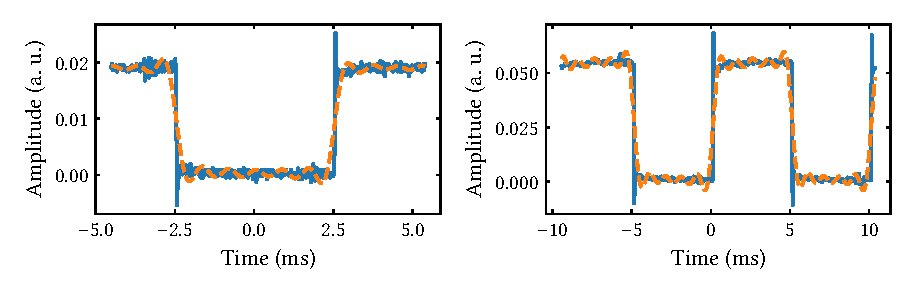
\includegraphics{figures/eom_extinction_155.pdf}
}
\caption{Measurements of extinction ratio for \ac{rtp} (left) and \ac{bbo} (right). The dashed lines indicate the fourier series fit in order to find the high and low level of the signal. The results are $>108:1$ for \ac{rtp} and $>129:1$ for \ac{bbo}.}
\end{figure}
